\documentclass[b5paper, openany]{ctexbook}
\usepackage{zref-abspage}
\usepackage[margin=2.5cm]{geometry}


\usepackage{pifont}
\usepackage[perpage,symbol*]{footmisc}
\DefineFNsymbols{circled}{{\ding{192}}{\ding{193}}{\ding{194}}
{\ding{195}}{\ding{196}}{\ding{197}}{\ding{198}}{\ding{199}}{\ding{200}}{\ding{201}}}
\setfnsymbol{circled}



\usepackage{amsmath,amsfonts,mathrsfs,amssymb}
\usepackage{graphicx}

\usepackage[font=bf,labelfont=bf,labelsep=quad]{caption}

\usepackage{tikz}


\usepackage{ntheorem}
\theoremseparator{\;}



\usepackage{blkarray}
\usepackage{bm}
\usepackage[colorlinks=true, linkcolor=black]{hyperref}



\theoremstyle{plain}
\theoremheaderfont{\normalfont\bfseries} 
\theorembodyfont{\normalfont}


\usepackage[framemethod=tikz]{mdframed}


\newtheorem{example}{\bf 例}[chapter]
\newenvironment{solution}{\noindent {\bf 解:}}{}
\newenvironment{analyze}{\noindent {\bf 分析:}}{}
\newenvironment{rmk}{ {\bf 注意:}}{}
\newenvironment{note}{ {\bf 说明:}}{}
\newenvironment{remark}{ {\bf 评述:}}{}

\renewcommand{\emptyset}{\varnothing}

\renewcommand{\proofname}{\bf 证明:}
\newenvironment{proof}{{\noindent \bf 证明:}}{}%{\hfill $\square$\par}

\newcommand{\E}{\mathbb{E}}
\renewcommand{\Pr}{\mathbb{P}}

\newcommand{\dif}{\,{\rm d}}
\newcommand{\Var}{{\rm Var}}
\newcommand{\Cov}{{\rm Cov}}
\newcommand{\x}{\times}
\renewcommand{\Longrightarrow}{\;\Rightarrow\;}
\newcommand{\map}[3]{#1:\; #2\mapsto #3}
\newcommand{\arccot}{{\rm arccot\,}}


 \usepackage{tcolorbox}
 \tcbuselibrary{breakable}
 \tcbuselibrary{most}



\newtcolorbox{ex}[1][]
  {colback = white, colframe = cyan!75!black, fonttitle = \bfseries,
    colbacktitle = cyan!85!black, enhanced,
    attach boxed title to top center={yshift=-2mm},breakable, 
    title=练习, #1}

\newtcolorbox{blk}[1][]
  {colback = white, colframe = magenta!75!black, fonttitle = \bfseries,
    colbacktitle = magenta!85!black, enhanced,
    attach boxed title to top left={xshift=5mm, yshift=-2mm},breakable, 
    title=思考题, #1}

\newtcolorbox{thm}[2][]
  {colback = white, colframe = magenta!75!black, fonttitle = \bfseries,
    colbacktitle = magenta!85!black, enhanced,
    attach boxed title to top left={xshift=5mm, yshift=-2mm},breakable, 
    title=#2, #1}

% \newtcolorbox{note}[1][]
%   {colback = white, colframe = blue!75!black, fonttitle = \bfseries,
%     colbacktitle = blue!85!black, enhanced,
%     attach boxed title to top left={xshift=5mm, yshift=-2mm},breakable, 
%     title=说明, #1}



\setcounter{tocdepth}{1}

\setcounter{secnumdepth}{2}



% \ctexset {
% section = {
% 	name = {第,节},
%  	number = \chinese{section}},
% subsection = {
% 	name = {,、\hspace{-1em}},
% 	number = \chinese{subsection}
% },
% subsubsection = {
% 	name = {(,)\hspace{-1em}},
% 	number = \chinese{subsubsection},
% }
% }



\renewcommand{\contentsname}{目~~录}

\newcommand{\poly}{\polynomial[reciprocal]}
\newcommand{\Q}{\mathbb{Q}}
\newcommand{\R}{\mathbb{R}}
\newcommand{\N}{\mathbb{N}}
\newcommand{\Z}{\mathbb{Z}}


\usepackage{mathtools}

\setlength{\abovecaptionskip}{0.cm}
\setlength{\belowcaptionskip}{-0.cm}

\usetikzlibrary{decorations.pathmorphing, patterns}
\usetikzlibrary{calc, patterns, decorations.markings}
\usetikzlibrary{positioning, snakes, hobby}

\usepackage{lscape}

\usepackage{yhmath}
\usepackage{longdivision}
\usepackage{polynom}
\usepackage{polynomial}
\usepackage{cancel}

\renewcommand{\frac}{\dfrac}
\newcommand{\oc}{$^{\circ}{\rm C}$}
\newcommand{\blank}{\underline{\qquad}}

\usepackage{multicol}
\usepackage{cases}
% \usepackage{enumitem}
\usepackage{ulem}
\usepackage{enumerate}

\DeclareSymbolFont{ugmL}{OMX}{mdugm}{m}{n}
\DeclareMathAccent{\widearc}{\mathord}{ugmL}{"F3}

\usepackage{tkz-euclide}
\newcommand{\VEC}{\overrightarrow}
\usetikzlibrary{decorations.pathmorphing}


\begin{document}



\title{\Huge\bfseries 北京四中高中教学讲义\\三角(全一册)}



\author{\Large 北京四中教学处~~编}
\date{\Large 1994年11月}

\maketitle




\frontmatter

\chapter{出版说明}

当前,中学教学改革已经深入到课程设置和教材改革领域。
我校数学教材的改革,以发展学生的数学思维为目标,以不改变现行教学大纲规定的教学闪容为前提,试图通过对知识结构及其展开方式的统盘考虑,实现整体优化。经多年反复探索、实验,编成了这套尝试融教材与教法、学法于一体的《北京四中高中教学讲义》。

这套讲义的产生可以上溯到 1982 年。从那时起,为了发展学生智能,提高数学素养,我校部分同志就开始对高中数学教学进行以教材改革为龙头,以学法教育为重点的“整体优化实验研究”。正是在这项研究的基础上,逐步形成了这套讲义编写的特色和风格。这就是:
\begin{enumerate}
    \item 为形成学生良好的认知结构,讲义的知识结构力求脉络分明,使学生能从整体上理解教材。
    \item 为了提高学生的数学素养,本讲义把数学思想的阐述放到了重要位置。数学思想既包含对数学知识点(概念、定理、公式、法则和方法)的本质认识,也包含对问题解决的数学基本观点。它是数学中的精华,对形成和发展学生的数学能力具有特别重要的意义。为此,讲义注重展现思维过程(概念、法则被概括的过程,教学关系被抽象的过程,解题思路探索形成的过程)。在过程中认识知识点的本质,在过程中总结思维规律,在过程中揭示数学思想的指导作用。力图使学生能深刻领悟教材。
    \item “再创造,再发现”在数学学习中对培养创造维能力至关重要,为引导学生积极参与“发现”,讲义在设计上做了某些尝试。
    \item 例题和习题的选配,力求典型、适量、成龙配套。习题分为 A 组(基本题)、 B 组(提高题)和 C 组(研究题)。教师可根据学生不同的学习水平适当选用。
    \item 教材是学生学习的依据。应有利于培养自学能力,本书注重启迪学法,并在书末附有全部习题的答案或提示,以供学习时参考。
 \end{enumerate}   

这套讲义在研究、试教和成书的过程中,始终得到了北京市和西城区教育部门有关领导的关怀和帮助,得到了北京师范大学数学系钟善基教授、曹才翰教授的热情指导,清华附中的瞿宁远老师也积极参与了我们的实验研究,并对这套教材做出了贡献,在此一并致以诚挚的谢意。

在编写过程中,北京四中数学组的教师们积极参加研讨,对他们的热情支持表示感谢。

这套讲义包括六册:高中代数第一、二、三册,三角、立体几何、解析几何各一册。

编写适应素质教育的教材,对我们来说是个尝试。由于水平所限,书中不当之处在所难免,诚恳希望专家、同行和同学们提出宝贵意见。

\begin{flushright}
    北京四中教学处\\
    1994年11月
\end{flushright}
\tableofcontents


\mainmatter

 
\begin{landscape}
\begin{tikzpicture}[>=stealth]
  
\node(H) at (0,0)[right, rectangle, draw]{积化和差与和差化积};
\node(G) at (0,1.5)[right, rectangle, draw]{万能公式};
\node(F) at (0,3)[right, rectangle, draw]{倍角公式};
\node(E) at (0,4.5)[right, rectangle, draw]{半角公式};
\draw[->, very thick ](F)--(G);
\draw[->, very thick](F)--(E);

\node(A) at (0,8)[draw, right, align=center, rectangle, text width=3cm]{角的度量\\(角度制与弧度制)};
\node(B) at (0,6.5)[draw, right, align=center, rectangle, text width=3cm]{角的概念的推广};
\draw[->, very thick](A)--(B);

\node (C) at (4.5,7)[draw, right, align=center, rectangle, text width=2.7cm]{任意角\\三角函数的定义\\(第一章)};
\node (D) at (8,7)[draw, right, align=center, rectangle, text width=2cm]{三角函数线\\及三角函数\\的某些性质};
\draw[->, very thick](C)--(D);

\node (I) at (4.5,4.5)[draw, right, align=center, rectangle, text width=2.7cm]{同角三角函数\\的基本公式};
\node (J) at (8,4.5)[draw, right, align=center, rectangle, text width=2cm]{诱导公式};

\draw[->, very thick](C)--(I);
\draw[->, very thick](D)--(J);
\draw[->, very thick](I)--(J);

\node (K) at (3,2.5)[draw, right, align=center, rectangle, text width=5cm]{和(差)的正弦、余弦、正切\\(第二章)};

\node (L) at (4,0)[draw, right, align=center, rectangle, text width=4cm]{$a\sin\alpha+b\cos\alpha=\sqrt{a^2+b^2}\sin(\alpha+\beta)$};

\draw[->, very thick](K)--(L);
\draw[->, very thick](K)--(F);
\draw[->, very thick](K)--(H);

\draw[->, very thick](I)--(K);
\draw[->, very thick](J)--(K);


\node (O) at (12,-.5)[draw, right, align=center, rectangle, text width=2.5cm]{三角方程\\(第五章)};
\node (N) at (12,3)[draw, right, align=center, rectangle, text width=2.5cm]{反三角函数\\(第四章)};
\node (M) at (12,7)[draw, right, align=center, rectangle, text width=2.5cm]{三角函数的性质和图象\\(第三章)};
\draw[->, very thick](D)--(M);
\draw[->, very thick](M)--(N);
\draw[->, very thick](N)--(O);

\draw[dashed](-0.5,6) rectangle (3.5,9);
\draw[dashed](-0.5,-1) rectangle (11,5.5);
\draw[dashed](4,5.75) rectangle (10.5 ,8.25);
\draw[->, very thick](11,1)--(O);
\draw[->, very thick](11,2.5)--(N);
\draw[->, very thick](11,4.5)--(M);
\draw[->, very thick](3.5,7)--(C);
\draw[->, very thick](4.15,5.75)--+(0,-2.6);

\end{tikzpicture}
\end{landscape}


\chapter{三角函数}
在初中,我们学习过三角函数的初步知识,重点研究的是用三角函数的定义解三角形(包括解直角三角形和解斜三角形).

本书将主要研究三角函数的性质、图象、运算(又称\textbf{三角变换})及其应用。这些知识对高中和大学的数学、物理的学习都是必备的基础。为了使同学们从整体上对上述内容的展开先有个粗略的了解,在下页我们画出了全书的理论结构框图。在学习过程中,经常翻阅它有助于了解所学知识点在整个知识体系中的地位、作用以及知识点之间的联系。

本章在扩充角的概念的基础上,首先建立任意角三角函数的定义,并对它的一些性质做初步的研究,最后讲一点应用。

\section{弧度制}
\subsection{角的度量单位}
三角函数的自变量是角。要从数量上刻画角的大小,首先碰到的问题是角的度量单位。同学们已经学过\textbf{角度制}。它的规定是:
周角的$\frac{1}{360}$叫做1度角,记作$1^{\circ}$。

于是,
\begin{equation}
\text{周角}\mathop{=}^{\text{度量}}360^{\circ},\qquad \text{平角}\mathop{=}^{\text{度量}}180^{\circ} \tag{1}
\end{equation}

现在,学习科学技术使用更加广泛的是“弧度制”,它规定:等于半径长的圆弧所对的圆心角叫做\textbf{1弧度角}。如图1.1,$\widearc{AB}$的长等于半径$r$,$\widearc{AB}$所对的圆心角$\angle AOB$就是1弧度角。在图1.2中,$\widearc{AC}$的长$\ell=2r$,$\widearc{AC}$所对的圆心角$\angle AOC$就是2弧度角。

\noindent
\begin{minipage}{.3\textwidth}
\begin{tikzpicture}
\draw (0,0) circle (1.5);
\draw[very thick](180/3.1416:1.5)node[above right]{$B$}--(0,0)node[below left]{$O$}--node[below]{$r$}(1.5,0)node[right]{$A$};
\node at (90/3.1416:1.5)[right]{$r$};
\draw(.5,0) arc (0:180/3.1416:.5)node[right]{1弧度};
\end{tikzpicture}
\captionof{figure}{}
\end{minipage}\hfill
\begin{minipage}{.3\textwidth}
    \begin{tikzpicture}
    \draw (0,0) circle (1.5);
\draw[very thick](360/3.1416:1.5)node[above left]{$C$}--(0,0)node[below left]{$O$}--node[below]{$r$}(1.5,0)node[right]{$A$};
\node at (180/3.1416:1.5)[above right]{$\ell=2r$};
\draw(.35,0) arc (0:360/3.1416:.35)node[above right]{2弧度};
\end{tikzpicture}
\captionof{figure}{}
\end{minipage}\hfill 
\begin{minipage}{.3\textwidth}
    \begin{tikzpicture}
    \draw (0,0) circle (1.5);
\draw[very thick](180:1.5)node[left]{$B$}--(0,0)node[below]{$O$}--node[below]{$r$}(1.5,0)node[right]{$A$};
\node at (0,1.5)[above]{$\ell=\pi r$};
\draw(.25,0) arc (0:180:.25);
\node at (0,.3)[above]{$\pi$弧度};
\end{tikzpicture}
\captionof{figure}{}
\end{minipage}

一般地,若圆心角$\alpha$所对的弧长为$\ell$,那么角$\alpha$的弧度数就是$\frac{\ell}{r}$,即
\begin{equation}
    \alpha=\frac{\ell}{r}\; \text{弧度} \tag{2}
\end{equation}
特别地,当$\ell=2\pi r$时(即弧长是一个整圆),此时的圆心角为周角,它的弧度数就是
\[\frac{\ell}{r}=\frac{2\pi r}{r}=2\pi\; \text{弧度}\]
这就是说,
\begin{equation}
 \text{周角} \mathop{=}^{\text{度量}} 2\pi\text{弧度},\qquad \text{平角}\mathop{=}^{\text{度量}}\pi \text{弧度} \quad  \text{(图1.3)} \tag{3}
\end{equation}

至此,一个明显的问题产生了:对于同一个角,当分别用“弧度”和“度”为单位度量时,所得的量数一般是不同的。
那么,怎样进行换算呢?比较(1)(3)可以看出:
\[\pi \text{弧度}=180^\circ\]
这就是两种单位制之间的换算关系式. 由此,
\[\begin{split}
    1\text{弧度}&=\left(\frac{180}{\pi}\right)^{\circ}\approx 57^{\circ}18',\\
1^{\circ}&=\frac{\pi}{180}\text{弧度}\approx 0.01745\text{弧度}.
\end{split}\]

\begin{example}
    把$67^{\circ}30'$化成弧度。
\end{example}

\begin{solution}
\[67^{\circ}30^{\prime}=\left(67\frac{1}{2}\right)^{\circ}=\frac{\pi}{180}\text{弧度}\times67\frac{1}{2}=\frac{3}{8}\pi\text{弧度}\]
\end{solution}

\begin{example}
    把$\frac{3}{5}\pi$弧度化成度.
\end{example}

\begin{solution}
\[\frac{3}{5}\pi\text{弧度}=\frac{3}{5}(\pi\text{弧度})=\frac{3}{5}\times180^{\circ}=108^{\circ}\]
\end{solution}

\begin{note}
今后用弧度表示角的时候,“弧度”二字通常略去不写,而只写这个角的弧度数。例如,角$\alpha=2$就表示$\alpha$是 2 弧度的角,$\frac\pi4$弧度的角$\alpha$就写成 $\alpha = \frac \pi 4$。在这种约定下, $\sin\frac\pi3$与$\cos\frac\pi2$分别表示$\frac\pi3$弧度的正弦与$\frac\pi2$弧度的余弦。
\end{note}

\begin{ex}
请填出下列特殊角的弧度数。
\begin{center}
\begin{tabular}{c|c|c|c|c|c|c|c}
\hline
度& $30^{\circ}$& $45^{\circ}$& $60^{\circ}$& $90^{\circ}$& $180^{\circ}$& $270^{\circ}$& $360^{\circ}$\\
\hline
弧度 &&&&&$\pi$&&\\
\hline
\end{tabular}
\end{center}
\end{ex}

\section*{习题一}
\begin{center}
    \bfseries A
\end{center}

\begin{enumerate}
    \item (口答)下列弧度各是多少度?
\begin{multicols}{4}
\begin{enumerate}[(1)]
    \item $\pi$
    \item $2\pi$
    \item $\frac{\pi}{2}$
    \item $\frac{\pi}{3}$
    \item $\frac{2\pi}{3}$
    \item $\frac{\pi}{4}$
    \item $\frac{3\pi}{4}$
    \item $\frac{7\pi}{4}$
    \item $\frac{\pi}{6}$
    \item $\frac{5\pi}{6}$
    \item $\frac{7\pi}{6}$
    \item $\frac{11\pi}{6}$
\end{enumerate}
\end{multicols}

\item 把下列各度化成弧度(写成多少$\pi$的形式):
\begin{multicols}{3}
\begin{enumerate}[(1)]
    \item $12^{\circ }$
    \item $75^{\circ }$
    \item $210^{\circ }$
    \item $135^{\circ }$
    \item $300^{\circ }$
    \item $22^{\circ }30'$
\end{enumerate}
\end{multicols}
\item 把下列各弧度化成度。
\begin{multicols}{3}
\begin{enumerate}[(1)]
    \item $\frac{\pi}{12}$
    \item $\frac{3\pi}{10}$
    \item $\frac{\pi}{5}$
    \item $\frac{4\pi}{3}$
    \item $\frac{\pi}{8}$
    \item $3$
\end{enumerate}
\end{multicols}

\item 求下列各三角函数的值:
\begin{multicols}{4}
\begin{enumerate}[(1)]
    \item $\sin\frac{2\pi}{3}$
    \item $\tan\frac{\pi}{6}$
    \item $\cos\frac{3}{4}\pi$
    \item $\sin 1$
\end{enumerate}
\end{multicols}

\item 填写下表中各个三角函数的值:
\begin{center}
\begin{tabular}{c|cccc}
\hline
&  正弦  &  余弦  & 正切  & 余切\\
\hline
$\frac{\pi}{6}$ &\\ [1.5ex]
$\frac{\pi}{4}$ &\\ [1.5ex]
$\frac{\pi}{3}$ &\\  [1.5ex]
\hline
\end{tabular}
\end{center}


\item 填写下表中各个三角函数的值:
\begin{center}
    \begin{tabular}{c|cccc}
    \hline
    &  正弦  &  余弦  & 正切  & 余切\\
    \hline
    $\frac{\pi}{2}$ &\\[1.5ex]
    $\frac{2\pi}{3}$ &\\[1.5ex]
    $\frac{3\pi}{4}$ &\\[1.5ex]
    $\frac{5\pi}{6}$ &\\[1.5ex]
    \hline
    \end{tabular}
    \end{center}
\end{enumerate}

\section{角的概念的推广}
在初中,我们所学过的角都是限制在$[0^{\circ}, 360^{\circ}]$之中。本节将把角的概念加以推广。

角可看作是由一条射线绕它的端点旋转而成的。如图
1.4,平面上射线$OA$绕它的端点$O$旋转到$OB$处便形成了角$\alpha$。射线$OA$叫做角$\alpha$的\textbf{始边},射线$OB$叫做角$\alpha$的\textbf{终边},射线的端点$O$叫做角的\textbf{顶点}。在始边逆时针旋转第一圈的过程中便形成了$0^{\circ}\sim  360^{\circ}$(即$0\sim 2\pi$)的所有角;继续旋转第二圈的过程中又形成了$360^{\circ}\sim  720^{\circ}$的所有角(图1.5);继续旋转下去可以形成任意大的角。

\noindent
\begin{minipage}{.4\textwidth}
\begin{tikzpicture}[>=stealth]
\draw[very thick](45:3)node[left]{$B$}--(0,0)node[left]{$O$}--(3,0)node[right]{$A$};
\draw[->](.5,0) arc (0:45:.5)node[below right]{$\alpha$};
\end{tikzpicture}    
\captionof{figure}{}
\end{minipage}\hfill
\begin{minipage}{.4\textwidth}
    \begin{tikzpicture}[>=stealth]
\draw[very thick](120:2)node[left]{$B$}--(0,0)node[left]{$O$}--(3,0)node[right]{$A$};
\draw[very thick](.5,0) arc (0:120:.5);
\draw[very thick](120:.5) arc (120:270:.65);
\draw[very thick](270:.8) arc (270:360:.9);
\draw[->, very thick](.9,0) arc (0:120:.9);
\node at (60:1)[right]{$\alpha$};
\end{tikzpicture}    
\captionof{figure}{}
    \end{minipage}

在实际生活中,角的形成有两种相反的旋转方向。除了上述逆时针方向外,按顺时针方向旋转也可以形成角。为了区别这两种旋转方向,我们把按逆时针旋转形成的角叫做\textbf{正角}。把按顺时针方向旋转形成的角叫做\textbf{负角}。如图1.6中,以$OA$为始边的角$\alpha=240^{\circ}$,$\beta=-120^{\circ}$, $\gamma=-585^{\circ}$.特别地,当射线$OA$没有做任何旋转时,我们也认为这时形成了一个角,并把这个角叫做\textbf{零角}。当射线逆时针旋转不足一圈时所形成的角叫做\textbf{周内角}。显然周内角的取值范围是$[0,2\pi)$。角的概念经这样推广后,它包括任意大小的正角、负角和零角。

\begin{figure}[htp]
    \centering
\begin{tikzpicture}[>=stealth]
\draw(-120:3.5)node[right]{$B_1$}--(0,0)node[below]{$O$}--(4,0)node[right]{$A$};
\draw(0,0)--(135:3.5)node[left]{$B_2$};
\draw[->, thick](2.5,0) arc  (0:-120:2.5);
\node at (-60:2.5)[fill=white]{$\beta=-120^{\circ}$};
\draw[->, thick](.5,0) arc  (0:240:.5);
\node at (120:.5)[above]{$\alpha=240^{\circ}$};
\draw[very thick](1,0) arc (0:-120:1);
\draw[very thick](-120:1) arc (-120:-180-31:1.3);
\draw[very thick](135:1.35) arc (135:5:1.5);
\draw[very thick](1.6,0) arc (0:-114:1.8);
\draw[very thick, ->](-120:1.9) arc (-120:-180-45:1.9);
\node at (-2,-1)[fill=white]{$\gamma=-585^{\circ}$};
\end{tikzpicture}
    \caption{}
\end{figure}

在用弧度制度量角时,正角的弧度数为正数,负角的弧度数是负数,零角的弧度数是零。即\textbf{角的弧度数集合与实数集合$\R$可以建立一一对应的关系}:每一个角的弧度数对应唯
一确定的实数,反之,每一个实数对应唯一确定的角的弧度数。

\begin{figure}[htp]
    \centering
\begin{tikzpicture}[>=stealth]
\begin{scope}
\draw[->](-2.5,0)--(2.5,0)node[below]{$x$};
\draw[->](0,-2.5)node[below]{(1)}--(0,2.5)node[left]{$y$};
\node [below right]{$O$};
\draw[thick](0,0)--(30:2.5)node[above]{$B_1$};
\draw[->](1.5,0) arc (0:-330:1.5);
\node at (165:1.5)[left]{$-300^{\circ}$};
\node at (115:.6)[left]{$390^{\circ}$};
\draw[->, thick](1.8,0) arc (0:30:1.8)node[below right]{$30^{\circ}$};
\draw[very thick](0.5,0) arc (0:180:.5);
\draw[very thick](-.5,0) arc (180:360:.7);
\draw[very thick, ->](.9,0) arc (0:30:.9);
\end{scope}
\begin{scope}[xshift=6cm]
    \draw[->](-2.5,0)--(2.5,0)node[below]{$x$};
\draw[->](0,-2.5)node[below]{(2)}--(0,2.5)node[left]{$y$};
\node [below right]{$O$};
\draw[thick](0,0)--(-60:2.5)node[below]{$B_2$};
\draw[thick](0,0)--(-135:2.25)node[below left]{$B_3$};
\draw[->, thick](1.75,0) arc (0:300:1.75);
\draw[->, thick](1.5,0) arc (0:-60:1.5);
\node at (-30:1.5)[right]{$-60^{\circ}$};
\node at (-120:1.8)[below]{$300^{\circ}$};
\draw[very thick](.5,0) arc (0:180:.6);
\draw[very thick](-.7,0) arc (180:360:.8);
\draw[very thick](.9,0) arc (0:180:1);
\draw[very thick, ->](-1.1,0) arc (180:180+45:1.1) ;
\node at (-.85,.85)[fill=white]{$585^{\circ}$};
\end{scope}
\end{tikzpicture}
    \caption{}
\end{figure}


今后,我们经常在直角坐标系中研究角。使角的顶点与坐标原点重合,始边$OA$与$x$轴正半轴重合(图1.7),让$OA$逆时针或顺时针旋转就可以得到任意大小的角。如果角的终边落在第几象限,就说这个角是第几象限的角(或说这个角属于第几象限)。如图1.7(1)中的角$30^{\circ}$,$390^{\circ}$,$-330^{\circ}$都是第一象限的角;图1.7(2)中的$300^{\circ}$,$-60^{\circ}$的角都是第四象限的角;$585^{\circ}$的角是第三象限的角。如果角的终边落在坐标轴上,就认为这个角不属于任何象限(称这类角为轴上角)。

在图1.7(1)中我们发现:$390^{\circ}$的角与$-330^{\circ}$的角都与$30^{\circ}$的角终边相同。

\begin{thm}{问1}
试把与$30^{\circ}$的角终边相同的一切角的值表示出来。
\end{thm}

很明显,当且仅当$30^{\circ}$加上“周角”的整数倍时,所得到
的角
\begin{equation}
    30^{\circ}+360^{\circ}\cdot k\quad (k\in\Z) \tag{1}
\end{equation}
的终边必定与$30^{\circ}$的角的终边相同。

当$k=0$时,它表示$30^{\circ}$的角;当$k=1$时,它表示$390^{\circ}$的角;当$k=-1$时,它表示$-330^{\circ}$的角,等等。把这一结果写成一般形式有

\begin{thm}
    {定理} 角$\beta$与角$\alpha$终边相同的充要条件是
\[\beta=\alpha+2\pi k\quad (k\in\Z)\]
\end{thm}

特别地,当$\alpha$是一个周内角时,上述结论仍然成立。

\begin{example}
    把下列各角写成周内角加上周角的整数倍的形式:
\begin{multicols}{4}
\begin{enumerate}[(1)]
    \item $855^{\circ}$
    \item $\frac{19\pi}{2}$
    \item $-\frac{16\pi}{3}$
    \item $-1410^{\circ}$
\end{enumerate}
\end{multicols}
\end{example}

\begin{solution}
\begin{enumerate}[(1)]
    \item $855^{\circ}=135^{\circ}+360^{\circ}\x 2$
    \item $\frac{19\pi}{2}=\frac{16\pi+3\pi}{2}=\frac{3\pi}{2}+2\pi\x 4$
    \item $-\frac{16\pi}{3}=\frac{-18\pi+2\pi}{3}=\frac{2\pi}{3}+2\pi\x (-3)$
    \item $-1410^{\circ}=-1440^{\circ}+30^{\circ}=30^{\circ}+360^{\circ}\x (-4)$
\end{enumerate}
\end{solution}

\section*{习题二}
\begin{center}
    \bfseries A
\end{center}

\begin{enumerate}
    \item 把下列度化成弧度:
\begin{multicols}{4}
\begin{enumerate}[(1)]
    \item $18^{\circ }$
    \item $- 120^{\circ }$
    \item $735^{\circ }$
    \item $-12.5^{\circ}$
    \item $10^{\circ}$
    \item $-1080^{\circ}$
    \item $19^{\circ}48^{\prime}$
    \item $-9^{\circ}20^{\prime}$
\end{enumerate}
\end{multicols}
    
\item     把下列弧度化成度。
\begin{multicols}{4}
\begin{enumerate}[(1)]
    \item $- \frac {7\pi }6$
    \item $\frac {\pi} {15}$
    \item $\frac {5\pi} {8}$
    \item $-\frac {8\pi} {3}$
    \item $-5$
    \item $1.4$
    \item $-12\pi$
    \item $-100\pi$
\end{enumerate}
\end{multicols}
\item 把下列角化成“周内角$+$周角的整数倍”的形式。
\begin{multicols}{4}
\begin{enumerate}[(1)]
    \item $-315^{\circ}$
    \item $1200^{\circ}$
    \item $-720^{\circ}$
    \item $-3500^{\circ}$
    \item $\frac{39\pi}{2}$
    \item $-\frac{7\pi}{5}$
    \item $- \frac {76}3\pi$
    \item $- \frac {397}4\pi$
\end{enumerate}
\end{multicols}

\item     下列各组中的两个角的终边是否相同(要简述理由)?
\begin{multicols}{2}
\begin{enumerate}[(1)]
    \item    $3570^{\circ}$与$2130^{\circ}$
    \item $-875^{\circ}$与$565^{\circ}$
    \item $\frac{285\pi}{7}$与$\frac{397\pi}{7}$
    \item $-\frac{11\pi}{4}$与$\frac{25\pi}{4}$
\end{enumerate}
\end{multicols}
\end{enumerate}    

\begin{center}
    \bfseries B
\end{center}

\begin{enumerate}\setcounter{enumi}{4}
    \item 求证:$\alpha$与$\beta$的终边相同$\Longleftrightarrow \beta=\alpha+2k\pi \; (k\in\Z)$
\end{enumerate}


现在,我们研究轴上角和象限中的角的一般形式。

\begin{figure}[htp]
    \centering
\begin{tikzpicture}[>=stealth, scale=1.5]
    \draw[->](-2,0)--(2,0)node[right]{$x$};
    \draw[->](0,-2)--(0,2)node[right]{$y$};
\node[below left]{$O$};
\draw[->, very thick](.5,0) arc (0:90:.5);
\node at (.45,.45)[fill=white]{$\frac{\pi}{2}$};
\draw[->, very thick](1,0) arc (0:180:1);
\node at (-.7,.7)[fill=white]{$\pi$};
\draw[->, very thick](1.5,0)node[below]{$A$} arc (0:270:1.5); 
\node at (-1.2,-1.2)[fill=white]{$\frac{3\pi}{2}$};
\end{tikzpicture}
    \caption{}
\end{figure}

从图1.8可以看出,终边在轴上的周内角由小到大依次
是
\[0,\quad  \frac{\pi}{2},\quad \pi,\quad \frac{3\pi}{2}\]
将这些角各加上$2k\pi\; (k\in\mathbb{Z})$ 就得到了轴上的所有的角。由此可见:
\begin{itemize}
    \item 终边在$x$轴正半轴上的一切角可以写成$0+2k\pi\; (k\in\mathbb{Z})$;
    \item 终边在$x$轴负半轴上的一切角可以写成$\pi+2k\pi\; (k\in\mathbb{Z})$;
    \item 终边在$y$轴正半轴上的一切角可以写成$\frac{\pi}{2}+2k\pi\; (k\in \Z)$; 
    \item 终边在$y$轴负半轴上的一切角可以写成$\frac{3\pi}{2}+2k\pi\; (k\in \Z)$.
\end{itemize}
进而
\begin{itemize}
    \item 终边在$x$轴上的一切角可写成$k\pi\; (k\in \Z)$;
    \item 终边在$y$轴上的一切角可写成$\frac{\pi}{2}+k\pi\; (k\in \Z)$.
\end{itemize}
再进一步,
\begin{itemize}
    \item 所有的轴上角可写成$\frac{\pi}{2}\cdot k\; (k\in \Z)$.
\end{itemize}

\begin{thm}{思考题}
   终边在$y$轴负半轴上的一切角写成$-\frac{\pi}{2}+2k\pi\; (k\in\Z)$对吗? 
\end{thm}

如果以$\theta_1,\theta_2,\theta_3,\theta_4$分别表示第一、二、三、四象限中的角,那么它们的取值范围是
\[\begin{split}
    0+2k\pi<&\theta_1<\frac{\pi}{2}+2k\pi\\
    \frac{\pi}{2}+2k\pi<&\theta_2<\pi+2k\pi\\
    \pi+2k\pi<&\theta_3<\frac{3\pi}{2}+2k\pi\\
    \frac{3\pi}{2}+2k\pi<&\theta_4<2\pi+2k\pi\\
\end{split}\]
其中:$k\in\Z$.

\begin{note}
    为直观,各象限中的角在写法上通常以周内角为基础,再加上周角的整数倍。
\end{note}

\begin{example}
    第二象限中的角的一半是第几象限中的角?
\end{example}

\begin{solution}

    \noindent
\begin{minipage}{.55\textwidth}
$\because\quad$ 第二象限中的角$\theta_2$满足
\[ \frac{\pi}{2}+2k\pi<\theta_2<\pi+2k\pi\quad (k\in\Z)\]
$\therefore\quad \frac{\pi}{4}+k\pi<\frac{\theta_2}{2}<\frac{\pi}{2}+k\pi\quad (k\in\Z)$

由此式可知:
\begin{itemize}
    \item 当$k$为偶数时,$\frac{\theta_2}{2}$是第一象限中的角;
    \item 当$k$为奇数时,$\frac{\theta_2}{2}$是第三象限中的角(图1.9)。
\end{itemize}

$\therefore\quad $第一象限中的角的半角是第一或第三象限的角.    
\end{minipage}
\hfill
\begin{minipage}{.4\textwidth}
    \centering
\begin{tikzpicture}[>=stealth, scale=1.1]
\draw[->](-2,0)--(2.25,0)node[right]{$x$};
\draw[->](0,-2.5)--(0,2.5)node[left]{$y$};
\node [below right] {$O$};
\fill[pattern=north east lines](0,0)--(0,2.5)--(1.78,1.78)--cycle;
\fill[pattern=north west lines](0,0)--(0,-2.5)--(-1.78,-1.78)--cycle;
\node[fill=white] at (.1,1.5)[right]{\small $k$为偶数};
\node[fill=white] at (-.1,-1.5)[left]{\small $k$为奇数};
\draw[very thick](-1.8,-1.8)node[above]{$\frac{5\pi}{4}$}--(1.8,1.8)node[right]{$\frac{\pi}{4}$};
\end{tikzpicture}
\captionof{figure}{}
\end{minipage}
\end{solution}

\begin{remark}
    这类问题的思考方法是先求出$\frac{\theta}{2}$应满足的关系,再结合图形对整数$k$进行讨论.
\end{remark}

在实际问题中,有时需要计算弧长和扇形的面积。

设圆的半径为$R$(图1.10),$\widearc{AB}$所对的圆心角为$n^{\circ}\; (n>0)$,则:
\begin{itemize}
    \item $\widearc{AB}$的长  \[\ell=\frac{n}{360}\cdot 2\pi R\]
    \item 扇形$\widearc{AOB}$面积 \[S=\frac{n}{360}\cdot \pi R^2\]
    \item 若圆心角为$\alpha$弧度$(\alpha>0)$,则:$\widearc{AB}$的长 \[\ell=\frac{\alpha}{2\pi}\cdot 2\pi R=\alpha R\] (或由公式$\alpha=\ell/R$直接得出)
    \item 扇形$\widearc{AOB}$的面积 \[S=\frac{\alpha}{2\pi}\cdot \pi R^2=\frac{1}{2}\alpha R\cdot R=\frac{1}{2}\ell\cdot R\]
\end{itemize}


\noindent
\begin{minipage}{.45\textwidth}
\centering
\begin{tikzpicture}[>=stealth]
\draw[->](-2.5,0)--(2.5,0)node[right]{$x$};
\draw[->](0,-2.5)--(0,2.5)node[left]{$y$};
\draw[dashed](0,0)node [below right]{$O$} circle (1.5);
\draw[very thick](1.5,0)node[below right]{$A$} arc (0:60:1.5)node[above]{$B$};

\draw(0,0)--(60:1.5);
\draw[->](.5,0)node[above right]{$n^{\circ}$} arc (0:60:.5);
\node at (30:1.75){$\ell$};
\end{tikzpicture}
\captionof{figure}{}
\end{minipage}\hfill
\begin{minipage}{.45\textwidth}
\centering
\begin{tikzpicture}[>=stealth,scale=1.3]
\draw[very thick](45:2) arc (45:45+90:2);
\draw[very thick](45:3) arc (45:45+90:3);
\draw[very thick, dashed](45:2.5) arc (45:45+90:2.5);
\draw[thick](120:4)--(0,0)--(60:4);
\draw[->](0,0)--node[right]{$R=45$}(0,2.5);
\node at (60:2.5)[right]{$B$};
\node at (120:2.5)[left]{$A$};
\draw[<->](60:3.5) arc (60:120:3.5);
\node at (0,3.7){$60^{\circ}$};
\end{tikzpicture}
\captionof{figure}{}
\end{minipage}

\begin{example}
    如图1.11,求公路弯道部分$\widearc{AB}$的长(精确到1米,图中的长度是米)
\end{example}

\begin{solution}
$\because\quad \alpha=60^{\circ}=\frac{\pi}{3}$

$\therefore\quad \ell=\alpha R=\frac{\pi}{3}\cdot 45=3.14\x 15\approx 47\text{(米)}$

答:弯道部分$\widearc{AB}$的长约47米.
\end{solution}

\section*{习题三}
\begin{center}
    \bfseries A
\end{center}

\begin{enumerate}
    \item 把下列各角化成“周内角$+$周角的整数倍”的形式,并判定它们各是第几象限中的角或是在哪个坐标轴上的角:
\begin{multicols}{4}
\begin{enumerate}[(1)]
    \item $\frac{155\pi}{4}$
    \item $101\pi$
    \item $\frac{749\pi}{6}$
    \item $-\frac{338\pi}{3}$
    \item $-\frac{59\pi}{2}$
    \item $-\frac{148\pi}{5}$
    \item $-3900^{\circ}$
    \item $-265^{\circ}$
\end{enumerate}
\end{multicols}

\item 与$-\frac{26}{3}\pi$的角终边相同的角的一般形式是\blank,其中最
小的正角是\blank,最大的负角等于\blank.
\item 第四象限中的角的一半是第几象限角?

\item 填表:
\begin{center}
\begin{tabular}{c|c|c|c|c}
  \hline
    角$\theta$所属象限 &\; I\; & \; II\; &\; III&\; IV \\
    \hline
    角$\frac{\theta}{2}$应属的象限 &&&&\\
    \hline
\end{tabular}
\end{center}

\item 已知$(4k+1)\pi<\alpha<(4k+1)\pi+\frac{\pi}{6}\; (k\in\Z)$,
则$\alpha$,$\frac{\alpha}{2}$,$2\alpha$各属第几象限?
\item (口答) \begin{enumerate}[(1)]
\item 第二象限的角一定是钝角吗?
\item $y$轴正半轴上的角一定是直角吗?
\end{enumerate}

\item 
直径是20cm的轮子,每秒钟旋转45弧度,求轮子上一定点经过5秒钟所转过的弧长。
\item 航海罗盘将圆周分成32等份,把一份所对的圆心角的大小分别用度与弧度表示出来。
\item 某种蒸汽机上的飞轮直径为1.2m,每分钟按逆时针方向转300转,求:
\begin{enumerate}[(1)]
\item 飞轮每秒钟转过的弧度数;
\item 轮周上的一点每秒钟经过的弧长。
\end{enumerate}


\item 要在半径$OA=100$cm的圆形金属板上,截取一块$\widearc{AB}$的长为112cm的扇形板,应截取的圆心角$AOB$的度数是多少(精确到$1^{\circ}$)?
\item 已知$1^{\circ}$的圆心角所对的弧长为1m,这个圆的半径是多少?
\item 已知长50cm的弧所对的圆心角为$200^{\circ}$,求该弧所在圆的半径(精确到1cm)。
\item 回忆三角函数的定义,并口述$30^{\circ}$、$45^{\circ}$、$60^{\circ}$各三角函数的值。
\end{enumerate}

\begin{center}
    \bfseries B
\end{center}

\begin{enumerate}\setcounter{enumi}{13}
    \item 写出与$-\frac{5\pi}{3}$终边相同的角的集合$S$,并求出其中属于$[-100\pi, 100\pi)$的角共有多少个?
 \item    如图所示:动点$P$、$Q$同时从点$A(r,0)$出发沿圆周运动。点$P$按逆时针方向
    每秒钟转$\frac{\pi}{3}$弧度,点$Q$按
    顺时针方向每秒钟转$\frac{\pi}{6}$
    弧度,试求点$P,Q$第一次相遇时所用的时间,所在的位置及各自走过的弧长。
\end{enumerate}

\begin{figure}[htp]
    \centering
\begin{tikzpicture}[>=stealth]
    \draw[->](-2.5,0)--(2.5,0)node[right]{$x$};
    \draw[->](0,-2)--(0,2.5)node[left]{$y$};
    \draw[ thick](0,0)node [below left]{$O$} circle (1.5);
\draw[ thick, ->](1.5,0) arc (0:60:1.5)node[above]{$P$};
\draw[ thick, ->](1.5,0)node[below right]{$A$} arc (0:-30:1.5)node[right]{$Q$};
\draw[fill](1.5,0) circle(1.2pt);

\end{tikzpicture}
    \caption*{(第15题)}
\end{figure}

\section{任意角三角函数的定义}

\subsection{三角函数的定义}
在初中,大家学过的三角函数是这样定义的:设$P(x,y)$是角$\alpha\; (0\le \alpha<2\pi)$的终边$OB$上异于原点的任一点(图1.12),记$|OP|=r\; (r>0)$,则比值$\frac{y}{r},\; \frac{x}{r},\; \frac{y}{x},\; \frac{x}{y}$都是$\alpha$
的函数,依次记为
\[\sin\alpha=\frac{y}{r},\quad \cos\alpha=\frac{x}{r},\quad \tan\alpha=\frac{y}{x},\quad \cot\alpha=\frac{x}{y}\]

\noindent
\begin{minipage}{.45\textwidth}
\centering
\begin{tikzpicture}[>=stealth]
    \draw[->](-2.5,0)--(2.5,0)node[right]{$x$};
    \draw[->](0,-2)--(0,2.5)node[left]{$y$};
\draw[thick](0,0)node[below left]{$O$}--(120:2.5)node[left]{$B$};
\draw[->](.5,0) arc (0:120:.5);
\node at (.5,.5){$\alpha$};
\draw[dashed](-1.5/2,0)node[below]{$x$}--(-1.5/2, 1.5/2*1.732)node[left]{$P(x,y)$}--(0,1.5/2*1.732)node[right]{$y$};
\node at (-.5,1)[right]{$r$};
\end{tikzpicture}    
\captionof{figure}{}
\end{minipage}
\hfill
\begin{minipage}{.45\textwidth}
\centering
\begin{tikzpicture}[>=stealth]
    \draw[->](-2.5,0)--(2.5,0)node[right]{$x$};
    \draw[->](0,-2)--(0,2.5)node[left]{$y$};
    \draw[ thick](0,0)node [below left]{$O$} circle (1.5);
    \draw[thick](0,0)node[below left]{$O$}--(120:2.5)node[left]{$B$};
    \draw[->](.5,0) arc (0:120:.5);
\node at (.5,.5){$\alpha$};
    \draw[dashed](-1.5/2,0)node[below]{$x$}--(-1.5/2, 1.5/2*1.732)node[left]{$P(x,y)$}--(0,1.5/2*1.732)node[right]{$y$};


\end{tikzpicture}    
\captionof{figure}{}
\end{minipage}


在这个定义中,角$\alpha$的取值范围是$[0,2\pi)$。为今后的需要,现在把它推广到任意角的情况。同时为了研究三角函数的性质更加简便,我们把点$P(x,y)$取在角$\alpha$的终边$OB$与\textbf{单位圆}(以原点为圆心,半径为1的圆)的交点处(图1.13)。应注意,点$P$选在此处不会影响上述四个比值的大小。为叙述方便,今后我们把这个交点叫做角$\alpha$在单位圆上的对应点。于是得到

\begin{thm}
{定义} 设$\alpha$是一个任意角,它的终边$OP$与单位圆相交于点$P(x,y)$,称
\begin{itemize}
    \item $y$为$\alpha$的\textbf{正弦},记为$\sin\alpha=y$;
    \item $x$为$\alpha$的\textbf{余弦},记为$\cos\alpha=x$;
    \item $\frac{y}{x}$为$\alpha$的\textbf{正切},记为$\tan\alpha=\frac{y}{x}$;
    \item $\frac{x}{y}$为$\alpha$的\textbf{余切},记为$\cot\alpha=\frac{x}{y}$;
 \item $\frac{1}{x}$为$\alpha$的\textbf{正割},记为$\sec\alpha=\frac{1}{x}$;
\item $\frac{1}{y}$为$\alpha$的\textbf{余割},记为$\csc\alpha=\frac{1}{y}$.
\end{itemize}
\end{thm}

\begin{note}
当角$\alpha$给定以后,$x$、$y$都被唯一确定,从而上述六个代数式$y$, $x$, $\frac{y}{x}$, $\frac{x}{y}$, $\frac{1}{x}$, $\frac{1}{y}$的值除去有时分母为零以外都是唯一确定的。所以,它们都是$\alpha$的函数。这些函数统称\textbf{三角函数}。
\end{note}

\begin{example}
    求下列各角$\alpha$的六个三角函数值:
\begin{multicols}{4}
\begin{enumerate}[(1)]
    \item $0$
    \item $\frac{\pi}{2}$
    \item $\pi$
    \item $\frac{3\pi}{2}$
\end{enumerate}
\end{multicols}
\end{example}

\begin{solution}
作单位圆,标出这些角对应的点(图1.14)
\begin{figure}[htp]
    \centering
\begin{tikzpicture}[>=stealth]
    \draw[->](-2.5,0)--(2.5,0)node[right]{$x$};
    \draw[->](0,-2)--(0,2.5)node[left]{$y$};
    \draw[ thick](0,0)node [below left]{$O$} circle (1.5);
    \node at (1.5,0)[above right]{$A(1,0)$};
    \node at (-1.5,0)[above left]{$C(-1,0)$};
    \node at (0,1.5)[above right]{$B(0,1)$};
    \node at (0,-1.5)[below right]{$D(0,-1)$};
\end{tikzpicture}
    \caption{}
\end{figure}
\begin{enumerate}[(1)]
    \item $\alpha=0$对应的点为$A(1,0)$,即$x=1$, $y=0$
    
$\therefore\quad \sin 0=0, \; \cos 0=1,\; \tan 0=0,\; \cot0\text{不存在},\; \sec0=1,\; \csc0\text{不存在}$

\item $\alpha=\frac{\pi}{2}$对应的点为$B(0,1)$,即$x=0$, $y=1$
    
$\therefore\quad \sin \frac{\pi}{2}=1, \; \cos \frac{\pi}{2}=0,\; \tan \frac{\pi}{2}\text{不存在},\; \cot\frac{\pi}{2}=0,$

$\sec\frac{\pi}{2}\text{不存在},\; \csc\frac{\pi}{2}=1$

\item $\alpha=\pi$对应的点为$C(-1,0)$,即$x=-1$, $y=0$
    
$\therefore\quad \sin \pi=0, \; \cos \pi=-1,\; \tan \pi=0,\; \cot\pi\text{不存在},\; \sec\pi=-1,\; \csc\pi\text{不存在}$

\item $\alpha=\frac{3\pi}{2}$对应的点为$D(0,-1)$,即$x=0$, $y=-1$
    
$\therefore\quad \sin \frac{3\pi}{2}=-1, \; \cos \frac{3\pi}{2}=0,\; \tan \frac{3\pi}{2}\text{不存在},\; \cot\frac{3\pi}{2}=0,$

$\sec\frac{3\pi}{2}\text{不存在},\; \csc\frac{3\pi}{2}=-1$
\end{enumerate}
\end{solution}

\begin{example}
求下列各角的六个三角函数的值:
\begin{multicols}{4}
\begin{enumerate}[(1)]
    \item $\frac{\pi}{3}$
    \item $\frac{3\pi}{4}$
    \item $\frac{5\pi}{4}$
    \item $\frac{5\pi}{3}$
\end{enumerate}
\end{multicols}
\end{example}

\begin{solution}
作单位圆,标出这些角对应的点(图1.15)
\begin{figure}[htp]
    \centering
\begin{tikzpicture}[>=stealth]
    \draw[->](-2.5,0)--(2.5,0)node[right]{$x$};
    \draw[->](0,-2)--(0,2.5)node[left]{$y$};
    \draw[](0,0)node [below left]{$O$} circle (1.5);
    \draw[very thick](0,0)-- (60:1.5)node [above right]{$P$};
    \draw[very thick](0,0)-- (135:1.5)node [above left]{$Q$};
    \draw[very thick](0,0)-- (-135:1.5)node [below left]{$R$};
    \draw[very thick](0,0)-- (-60:1.5)node [below right]{$S$};
    \draw[dashed](60:1.5)--(-60:1.5);
    \draw[->](.5,0) arc (0:60:.5)node[right]{\small $\frac{\pi}{3}$};
\end{tikzpicture}
    \caption{}
\end{figure}

\begin{enumerate}[(1)]
    \item $\frac{\pi}{3}$对应的点为$P\left(\frac{1}{2},\frac{\sqrt{3}}{2}\right)$,

$\therefore\quad \sin\frac{\pi}{3}=\frac{\sqrt{3}}{2},\quad \cos\frac{\pi}{3}=\frac{1}{2},\quad \tan\frac{\pi}{3}=\sqrt{3},\quad \cot\frac{\pi}{3}=\frac{\sqrt{3}}{3}$

$\sec\frac{\pi}{3}=2,\quad \csc\frac{\pi}{3}=\frac{2}{3}\sqrt{3}$

\item $\frac{3\pi}{4}$对应的点为$Q\left(-\frac{\sqrt{2}}{2},\frac{\sqrt{2}}{2}\right)$,

$\therefore\quad \sin\frac{3\pi}{4}=\frac{\sqrt{2}}{2},\quad \cos\frac{3\pi}{4}=-\frac{\sqrt{2}}{2},\quad \tan\frac{3\pi}{4}=-1,\quad \cot\frac{3\pi}{4}=-1$

$\sec\frac{3\pi}{4}=-\sqrt{2},\quad \csc\frac{3\pi}{4}=\sqrt{2}$


\item $\frac{5\pi}{4}$对应的点为$R\left(-\frac{\sqrt{2}}{2},-\frac{\sqrt{2}}{2}\right)$,

$\therefore\quad \sin\frac{5\pi}{4}=-\frac{\sqrt{2}}{2},\quad \cos\frac{5\pi}{4}=-\frac{\sqrt{2}}{2},\quad \tan\frac{5\pi}{4}=1,\quad \cot\frac{5\pi}{4}=1$

$\sec\frac{5\pi}{4}=-\sqrt{2},\quad \csc\frac{5\pi}{4}=-\sqrt{2}$

\item $\frac{5\pi}{3}$对应的点为$S\left(\frac{1}{2},-\frac{\sqrt{3}}{2}\right)$,

$\therefore\quad \sin\frac{5\pi}{3}=-\frac{\sqrt{3}}{2},\quad \cos\frac{5\pi}{3}=\frac{1}{2},\quad \tan\frac{5\pi}{3}=-\sqrt{3},\quad \cot\frac{5\pi}{3}=-\frac{\sqrt{3}}{3}$

$\sec\frac{5\pi}{3}=2,\quad \csc\frac{5\pi}{3}=-\frac{2\sqrt{3}}{3}$
\end{enumerate}    
\end{solution}

\subsection{三角函数值的几何表示——三角函数线}
先简介有向线段的概念。

我们知道,坐标轴是规定了方向的直线。线段也可以规
定方向。如图1.16中,在$x$轴上的线段$AB$就可以规定两种相反的方向:以$A$为始点以$B$为终点(记为$\VEC{AB}$),或者以$B$为始点以$A$为终点(记为$\VEC{BA}$)。同样,与$y$轴平行的线段$CD$也
可以规定两种方向:以$C$为始点以$D$为终点(记为$\VEC{CD}$),或者以$D$为始点以$C$为终点(记为$\VEC{DC}$)。如果这条线段的方向与坐标轴的正方向相一致,我们规定用一个正数来表示它,否则就用一个负数来表示它。如上述有向线段可以分别表示成$\VEC{AB}=+3$,$\VEC{BA}=-3$,$\VEC{CD}=-4$,$\VEC{DC}=+4$等。象这样规定了方向的线段,称为\textbf{有向线段}。

现在,我们用有向线段来表示三角函数的值。

\noindent
\begin{minipage}{.45\textwidth}
    \centering
\begin{tikzpicture}[>=stealth, scale=.5]
\draw[->](-4,0)--(5,0)node[below]{$x$};
\draw[->](0,-5)--(0,5)node[left]{$y$};
\foreach \x in {-1,-2,-3,-4,1,2,3,4}
{
    \draw(\x,0)--(\x,.2);
    \draw(0,\x)--(.2,\x);
}
\draw[ultra thick](1,0)node[below]{$A$}--(4,0)node[below]{$B$};
\draw[ultra thick](-2,1)node[left]{$C$}--(-2,-3)node[left]{$D$};
\node [below left]{$O$};

\end{tikzpicture}
\captionof{figure}{}
\end{minipage}\hfill
\begin{minipage}{.45\textwidth}
    \centering
\begin{tikzpicture}[>=stealth]
    \draw[->](-2.5,0)--(2.5,0)node[right]{$x$};
    \draw[->](0,-2)--(0,2.5)node[left]{$y$};
    \draw(0,0)node [below left]{$O$} circle (1.5);
\tkzDefPoints{1.5/0/A, -1.5/0/B, 0/1.5/C, 0/-1.5/D}
\tkzLabelPoints[above left](B)
\tkzLabelPoints[above right](A,C)
\tkzLabelPoints[below right](D)
\draw(0,0)--(45:1.5)node[right]{$P(x,y)$};
\draw[dashed](0,1.5/1.414)node[left]{$M$}--(45:1.5)--(1.5/1.414,0)node[below]{$N$};
\draw[very thick, <->](0,1.5/1.414)--(0,0)--(1.5/1.414,0);
\draw[->](.5,0) arc (0:45:.5)node[right]{$\alpha$};
\end{tikzpicture}
\captionof{figure}{}
\end{minipage}


设角$\alpha$的终边与单位圆相交于$P(x,y)$. 过点$P$分别作$PM\bot y$轴于点$M$,$PN\bot x$轴于点$N$(图1.17)。则有向线段
\[\VEC{OM}=y,\qquad \VEC{ON}=x\]
因此,可以把$\VEC{OM}$和$\VEC{ON}$分别看作是$\sin\alpha=y$和$\cos\alpha=x$的几何形式。今后把$\VEC{OM}$叫做角$\alpha$的\textbf{正弦线},把正弦线所在的直径$\VEC{DC}$叫做\textbf{正弦轴}。同样,把$\VEC{ON}$叫做角$\alpha$的\textbf{余弦线},把余弦线所在直径$BA$叫做\textbf{余弦轴}.

\begin{thm}{思考题1}
    你能画出角$\alpha$的具有代表性的各种情况下的正弦线和余弦线吗?(提示:各有八种情况)
\end{thm}

\begin{thm}
{思考题2} 当角$\alpha$从0增加到$2\pi$时,试根据正弦线$\VEC{OM}$(余弦线$\VEC{ON}$)变化的规律,说出正弦值(余弦值)增、减变化的规律。
   
\end{thm}

现在研究正切值的几何形式。 

角$\alpha$的正切$\tan\alpha=\frac{y}{x}$,欲用一条有向线段表示比值$\frac{y}{x}$是困难的。为此,先作变形:
\begin{equation}
    \tan\alpha=\frac{y}{x}=\frac{\bar y}{1} \tag{*}
\end{equation}
从图1.18可以想到,只要能把$\bar y$表示出来,目标就达到了. 由比例式(*)可以看出,过点$A$作圆的切线$GG'$,连$OP$并延长与$GG'$交于$T$,有
\[\frac{y}{x}=\frac{\VEC{AT}}{OA}=\frac{\VEC{AT}}{1}=\VEC{AT}\]
由此,可以把$\VEC{AT}$叫做角$\alpha$的\textbf{正切线},$\VEC{AT}$所在的圆的切线$GG'$叫做\textbf{正切轴},其方向与$y$轴相同。应该注意的是$\VEC{AT}$的始点是点$A$。终点$T$是$OP$或其反向延长线与正切轴$G'G$的交点。

\begin{figure}[htp]
    \centering
\begin{tikzpicture}[>=stealth]
    \draw[->](-2,0)--(2.5,0)node[right]{$x$};
    \draw[->](0,-2)--(0,3.5)node[left]{$y$};
    \draw(0,0) circle (1.5);
\draw[very thick](-120:1.5)node[below left]{$P'(x',y')$}--(60:1.5)node[above]{$P(x,y)$};
\draw(60:1.5)--(60:3)node[right]{$T$};
\draw(1.5,3)node[above]{$G$}--(1.5,0)node[below right]{$A$}--(1.5,-2)node[right]{$G'$};
\draw[decorate, decoration={brace, amplitude=8pt}](1.5,1.5*1.732)--node[right=8pt]{$\bar y$}(1.5,0);

\node [above left]{$O$};
\draw[->](0.3,0) arc (0:60:.3)node[right]{$\alpha$};
\draw[dashed](1.5/2,0)node[below]{$N$}--node[right]{$y$}(60:1.5);
\node at (1.5/4,0)[below]{$x$};
\end{tikzpicture}
    \caption{}
\end{figure}


\begin{thm}
    {思考题3} 你能画出在各种情况下的具有代表性的正切线吗?(也有八种情况)
\end{thm}


\begin{thm}
    {思考题4} 当角$\alpha$从0增加到$2\pi$时,试根据$\VEC{AT}$的变化规律说出正切值增、减变化的规律。
\end{thm}

\begin{thm}
    {问1} 类比正切线的探寻过程,你能找到余切值的几何形式——余切线吗?
\end{thm}

事实上由
\[\cot\alpha=\frac{x}{y}=\frac{\bar x}{1}\]
由此想到过点$B$作圆的切线$C'C$,连$OP$并延长交$C'C$于$Q$,过$Q$作$QD\bot Ox$轴(图1.19),则$\VEC{OD}=\bar x$,从而
\[\frac{x}{y}=\VEC{OD}=\VEC{BQ}\]
我们把$\VEC{BQ}$叫做角$\alpha$的\textbf{余切线},$\VEC{BQ}$所在的圆的切线叫做\textbf{余切轴},它的方向与$x$轴同向。应该注意,余切线的始点为$B$,终点$Q$则是半径$OP$或其反向延长线与余切轴$CC'$的交点。

\begin{figure}[htp]
    \centering
\begin{tikzpicture}[>=stealth, scale=1.2]
    \draw[->](-3,0)--(4.5,0)node[right]{$x$};
    \draw[->](0,-2)--(0,2.5)node[left]{$y$};
    \draw(0,0)node[above left]{$O$} circle (1.5);
\draw[very thick](-150:1.5)--(30:1.5)node[right]{$P(x,y)$};
\draw(-2.5,1.5)node[left]{$C'$}--(4,1.5)node[right]{$C$};
\node at (0,1.5)[above right]{$B$};
\draw[dashed] (1.732*1.5,1.5)node[above]{$Q$}--(1.732*1.5,0)node[below]{$D$};
\draw[thick](1.732*1.5,1.5)--(30:1.5);
\draw[dashed](1.732*1.5/2, 0)--node[left]{$y$}(30:1.5);
\draw[thick](1.732*1.5/2, 0)--node[below]{$x$}(0,0);
\draw[->](.5,0) arc (0:30:.5)node[right]{$\alpha$};
\draw[decorate, decoration={brace, amplitude=8pt}](1.732*1.5,0)--node[below=8pt]{$\bar x$}(0,0);
\draw[decorate, decoration={brace, amplitude=8pt}](1.732*1.5,1.5)--node[right=8pt]{$1$}(1.732*1.5,0);
\end{tikzpicture}
    \caption{}
\end{figure}

\begin{thm}
{思考题5} 请画出在各种情况下具有代表性的余切线,并根据当角$\alpha$从0增加到$2\pi$时,余切线变化的规律说出余切值增、减变化的规律。
\end{thm}

以上,对$\sin\alpha$、$\cos\alpha$、$\tan\alpha$、$\cot\alpha$分别定义了它们的函数线。应明确:每种三角函数的定义及其相应的函数线之间的对应都是数与形的对应。如对$\sin\alpha=y$来说,$y$是它的代数形式,正弦线$\VEC{OM}$是它的几何形式。两种形式各具特色,各有所用,代数形式便于运算,几何形式形象直观。

\section*{习题四}
\begin{center}
    \bfseries A
\end{center}

\begin{enumerate}
    \item 填表:
\begin{center}
\begin{tabular}{c|c|c|c|c|c|c|c}
    \hline
$\alpha$ & 单位圆上 &$\sin\alpha$&$\cos\alpha$&$\tan\alpha$&$\cot\alpha$&$\sec\alpha$&$\csc\alpha$\\
&对应点的坐标是&&&&&& \\
\hline
$\frac{3\pi}{4}$ & $P_1(\qquad \qquad )$&&&&&& \\[1.5ex]
$\frac{5\pi}{4}$ & $P_2(\qquad \qquad )$&&&&&& \\[1.5ex]
$\frac{7\pi}{4}$ & $P_3(\qquad \qquad )$&&&&&& \\[1.5ex]
$\frac{2\pi}{3}$ & $P_4(\qquad \qquad )$&&&&&& \\[1.5ex]
$\frac{4\pi}{3}$ & $P_5(\qquad \qquad )$&&&&&& \\[1.5ex]
$\frac{5\pi}{6}$ & $P_6(\qquad \qquad )$&&&&&& \\[1.5ex]
$\frac{7\pi}{8}$ & $P_7(\qquad \qquad )$&&&&&& \\[1.5ex]
\hline
\end{tabular}
\end{center}    

\item 分别作出下列各角的正弦线、余弦线、正切线、余切线:
\begin{multicols}{4}
\begin{enumerate}[(1)]
    \item $\frac{\pi}{3}$
    \item $\frac{5\pi}{6}$
    \item $-\frac{2\pi}{3}$
    \item $-\frac{13\pi}{6}$
\end{enumerate}
\end{multicols}
\item 以2cm为“单位长”作单位圆,再分别作出角$\alpha$等于$\frac{\pi}{6}$、$\frac{5\pi}{4}$、$\frac{11\pi}{6}$
的正弦线、余弦线、正切线、余切线,量出它们的长度,据此长度把相应的正弦值、余弦值、正切值和余切值(精确到0.1)填入下表之中:
\begin{center}
\begin{tabular}{c|c|c|c|c}
\hline
角$\alpha$ & $\sin\alpha$&$\cos\alpha$&$\tan\alpha$&$\cot\alpha$\\
\hline
$\frac{\pi}{6}$ &&&&\\[1.5ex]
$\frac{5\pi}{4}$ &&&&\\[1.5ex]
$\frac{11\pi}{6}$ &&&&\\[1.5ex]
\hline
\end{tabular}
\end{center}
\end{enumerate}

\begin{center}
    \bfseries B
\end{center}

\begin{enumerate}\setcounter{enumi}{3}
    \item 仍以2cm为“单位长”作单位圆,再作出$\alpha=230^{\circ}$的正弦线、余弦线、正切线、余切线,量出其长,据此写出$\sin\alpha$、$\cos\alpha$、$\tan\alpha$、$\cot\alpha$的值。由此,你能悟出什么道理?
\end{enumerate}

\section{由定义和三角函数线观察三角函数的某些性质}
为了进行三角函数值的计算,本节对三角函数的某些性质先从直观上作初步的探究。

\subsection{定义域}

\noindent
\begin{minipage}{.45\textwidth}
\CTEXindent    根据三角函数的定义(图1.20)
\[\begin{split}
    \sin\alpha=y,&\quad \cos\alpha=x\\ 
    \tan\alpha=\frac{y}{x},&\quad \cot\alpha=\frac{x}{y}\\
    \sec\alpha=\frac{1}{x},&\quad \csc\alpha=\frac{1}{y}
\end{split}\]
可以看出:

对于正(余)弦,不论$\alpha$为何实数,整式$y$、$x$都有意义,

$\therefore\quad \sin\alpha,\; \cos\alpha$的定义域为$\alpha\in\R$;


\end{minipage}\hfill
\begin{minipage}{.45\textwidth}
\centering
\begin{tikzpicture}[>=stealth]
    \draw[->](-2.5,0)--(2.5,0)node[right]{$x$};
    \draw[->](0,-2)--(0,2.5)node[left]{$y$};
    \draw(0,0)node[below left]{$O$} circle (1.5);
\node at (1.5,0)[below right]{$A$};
\draw[very thick](0,0)--(120:1.5)node[left]{$P(x,y)$};
\draw[->](0.5,0) arc (0:120:.5);
\node at (60:.8){$\alpha$};
\end{tikzpicture}
\captionof{figure}{}
\end{minipage}

对于正切与正割,除去$y$轴上的点以外,分式$\frac{y}{x}$, $\frac{1}{x}$
都有意义,

$\therefore\quad \tan\alpha$的定义域为$\alpha\in\R$ 且$\alpha\ne \frac{\pi}{2}+k\pi\; (k\in\Z)$, 

对于余切与余割,除去$x$轴上的点以外,分式$\frac{x}{y}$, $\frac{1}{y}$都有意义,

$\therefore\quad \cot\alpha,\; \csc\alpha$的定义域为$a\in\R$,且$\alpha\ne k\pi\; (k\in\Z)$.

\subsection{函数值的符号和取值范围(函数的值域)}
从三角函数线的变化规律以及正(余)割的定义可以看出,当角$\alpha$在各自定义域上变化时,其函数值的取值范围如下表所示,其函数值在四个象限中的符号如图1.21所示。
\begin{center}
    \begin{tabular}{c|c|c|c}
\hline
函数名称& 定义式& 定义域& 值域\\
\hline
$\sin\alpha$ & $y$  &  $\alpha\in\R$ &  $[-1,\;1]$\\[1.5ex]
$\cos\alpha$ & $x$  &  $\alpha\in\R$ &  $[-1,\;1]$\\[1.5ex]
$\tan\alpha$ & $\frac{y}{x}$  &  $\alpha\in\R$且$\alpha\ne \frac{\pi}{2}+k\pi\; (k\in\Z)$ &  $(-\infty,\;+\infty)$\\[1.5ex]
$\cot\alpha$ & $\frac{x}{y}$  &  $\alpha\in\R$且$\alpha\ne k\pi\; (k\in\Z)$ &  $(-\infty,\;+\infty)$\\[1.5ex]
$\sec\alpha$ & $\frac{1}{x}$  &  $\alpha\in\R$且$\alpha\ne \frac{\pi}{2}+k\pi\; (k\in\Z)$ &  $(-\infty,-1]\cup[1,+\infty)$\\[1.5ex]
$\csc\alpha$ & $\frac{1}{y}$  &  $\alpha\in\R$且$\alpha\ne k\pi\; (k\in\Z)$ &  $(-\infty,-1]\cup[1, +\infty)$\\[1.5ex]
\hline
    \end{tabular}
\end{center}

\begin{figure}[htp]
    \centering
\begin{tikzpicture}[>=stealth, scale=1.1]
\begin{scope}
    \draw[->](-1.5,0)--(1.5,0)node[right]{$x$};
    \draw[->](0,-1.5)node[below]{$\sin\alpha$与$\csc\alpha$}--(0,1.5)node[left]{$y$};
    \draw(0,0)node[below left]{$O$} circle (1);
\node at (.5,.5){$+$};
\node at (-.5,.5){$+$};
\node at (.5,-.5){$-$};
\node at (-.5,-.5){$-$};
\end{scope}
\begin{scope}[xshift=4cm]
    \draw[->](-1.5,0)--(1.5,0)node[right]{$x$};
    \draw[->](0,-1.5)node[below]{$\cos\alpha$与$\sec\alpha$}--(0,1.5)node[left]{$y$};
    \draw(0,0)node[below left]{$O$} circle (1);
\node at (.5,.5){$+$};
\node at (-.5,.5){$-$};
\node at (.5,-.5){$+$};
\node at (-.5,-.5){$-$};
\end{scope}
\begin{scope}[xshift=8cm]
    \draw[->](-1.5,0)--(1.5,0)node[right]{$x$};
    \draw[->](0,-1.5)node[below]{$\tan\alpha$与$\cot\alpha$}--(0,1.5)node[left]{$y$};
    \draw(0,0)node[below left]{$O$} circle (1);
\node at (.5,.5){$+$};
\node at (-.5,.5){$-$};
\node at (.5,-.5){$-$};
\node at (-.5,-.5){$+$};
\end{scope}
\end{tikzpicture}
    \caption{}
\end{figure}

\subsection{诱导公式}
\subsubsection{$f(\alpha+2k\pi)$与$f(\alpha)$之间的关系}

为叙述方便,以下统一用$f(\alpha)$表示角$\alpha$的六个三角函数。欲求$f(\alpha+2k\pi)$与$f(\alpha)$之关系,只要弄清楚角$\alpha$与$\alpha+2k\pi\; (k\in\Z)$的对应点在单位圆上的位置关系就行了。据1.2节的定理,这两个对应点在单位圆上重合,即它们的直角坐标完全相同。
\[\therefore\quad f(\alpha+2k\pi)=f(\alpha)\]
这样,就得到了

\begin{thm}{公式(一)}
\[\begin{split}
\sin(\alpha+2k\pi)=\sin\alpha   &\qquad  \cos(\alpha+2k\pi)=\cos\alpha \\
\tan(\alpha+2k\pi)=\tan\alpha  &\qquad \cot(\alpha+2k\pi)=\cot\alpha \\
\sec(\alpha+2k\pi)=\sec\alpha  &\qquad \csc(\alpha+2k\pi)=\csc\alpha \\
\end{split}\]
其中,$k\in\Z$.
\end{thm}

由于“$2k\pi\; (k\in\Z)$”是周角的整数倍,这组公式表明:在计算三角函数值的时候,周角的整数倍可以“去掉”。特别地,当$\alpha$是周内角时,这组公式的功能在于:能把周外角的函数化为周内角的函数,从而能简化函数性质的研究和计算。

\subsubsection{$f(-\alpha)$与$f(\alpha)$之间的关系}

$\because\quad $角$\alpha$与$(-\alpha)$的对应点$P(x,y)$与$P'(x',y')$关于$x$轴对称(图1.22)

$\therefore\quad x=x',\quad y=-y'$

从而,得到:

\begin{thm}{公式(二)}
    \[\begin{split}
\sin(-\alpha)=-\sin\alpha   &\qquad  \cos(-\alpha)=+\cos\alpha \\
\tan(-\alpha)=-\tan\alpha  &\qquad \cot(-\alpha)=-\cot\alpha \\
\sec(-\alpha)=+\sec\alpha  &\qquad \csc(-\alpha)=-\csc\alpha \\
\end{split}\]
\end{thm}

这组公式的功能在于:能把负角的函数化为正角的函数,从而能简化函数性质的研究和计算。



\noindent
\begin{minipage}{.45\textwidth}
\begin{tikzpicture}[>=stealth]
    \draw[->](-2.5,0)--(2.5,0)node[right]{$x$};
    \draw[->](0,-2)--(0,2.5)node[left]{$y$};
    \draw(0,0)node[below right]{$O$} circle (1.5);
\draw[very thick](150:1.5)node[left]{$P(x,y)$}--(0,0)--(-150:1.5)node[left]{$P'(x',y')$};
\draw[dashed](150:1.5)--(-150:1.5);
\draw[->](.7,0) arc (0:150:.7);
\draw[->](.8,0) arc (0:-150:.8);
\node at (1.5,0)[below right]{$A$};
\node at (75:.9){$\alpha$};
\node at (-75:1){$-\alpha$};
\end{tikzpicture}
\captionof{figure}{}
\end{minipage}\hfill
\begin{minipage}{.45\textwidth}
\begin{tikzpicture}[>=stealth]
    \draw[->](-2.5,0)--(2.5,0)node[right]{$x$};
    \draw[->](0,-2)--(0,2.5)node[left]{$y$};
    \draw(0,0)node[below right]{$O$} circle (1.5);
\draw[very thick](210:1.5)node[left]{$P'(x',y')$}--(0,0)--(30:1.5)node[right]{$P(x,y)$};
\draw[->](.5,0) arc (0:210:.5);
\draw[->](.8,0) arc (0:30:.8);
\node at (105:.6)[left]{$\pi+\alpha$};
\node at (15:1){$\alpha$};
\end{tikzpicture}
\captionof{figure}{}
\end{minipage}


\subsubsection{$f(\pi+\alpha)$与$f(\alpha)$之间的关系}
$\because\quad $角$\alpha$与$(\pi+\alpha)$的对应点$P(x,y)$与$P'(x',y')$关于原点对称(图1.23)

$\therefore\quad x=-x',\quad y=-y'$

从而得到:

\begin{thm}{公式(三)}
\[\begin{split}
\sin(\pi+\alpha)=-\sin\alpha   &\qquad  \cos(\pi+\alpha)=-\cos\alpha \\
\tan(\pi+\alpha)=+\tan\alpha  &\qquad \cot(\pi+\alpha)=+\cot\alpha \\
\sec(\pi+\alpha)=-\sec\alpha  &\qquad \csc(\pi+\alpha)=-\csc\alpha \\
\end{split}\]
\end{thm}

这组公式的功能:能把$(\pi+\alpha)$的函数化为$\alpha$的函数,特别,当$\alpha$为锐角时,运用它能把第III象限的角$(\pi+\alpha$)的函数一举化成锐角的函数,从而能把函数简化。要记忆这组公式,关键是记住公式右边的符号——它是视$\alpha$为锐角时原来函数$f(\pi+\alpha)$的值的符号。

\subsubsection{$f(\pi-\alpha)$与$f(\alpha)$之间的关系}
$\because\quad $角$\alpha$与$(-\alpha)$的对应点P与Q关于x轴对称,而$(-\alpha)$与$(-\alpha+\pi)$的对应点$Q$与$P'$关于原点对称,从而$\alpha$与$(-\alpha+\pi)$的对应点$P(x,y)$与$P'(x',y')$关于$y$轴对称(图1.24)

$\therefore\quad 
x=-x',\quad y=y'$

这样,就得到:

\begin{thm}{公式(四)}
    \[\begin{split}
\sin(\pi-\alpha)=+\sin\alpha   &\qquad  \cos(\pi-\alpha)=-\cos\alpha \\
\tan(\pi-\alpha)=-\tan\alpha  &\qquad \cot(\pi-\alpha)=-\cot\alpha \\
\sec(\pi-\alpha)=-\sec\alpha  &\qquad \csc(\pi-\alpha)=+\csc\alpha \\
\end{split}\]
\end{thm}

\begin{thm}{思考题1}
    你能指出公式(四)的功能以及记忆它的方法吗?
\end{thm}

\begin{thm}{思考题2}
    在公式(三)中,以$(-\alpha)$代替$\alpha$,再用公式(二)也能导出公式(四),试试看,这种做法合理吗?
\end{thm}

\noindent
\begin{minipage}{.45\textwidth}
\begin{tikzpicture}[>=stealth]
    \draw[->](-2.5,0)--(2.5,0)node[right]{$x$};
    \draw[->](0,-2)--(0,2.5)node[left]{$y$};
    \draw(0,0)node[below left]{$O$} circle (1.5);
\draw[very thick](150:1.5)node[left]{$P'(x',y')$}--(0,0)--(30:1.5)node[right]{$P(x,y)$};
\draw[dashed](0,0)--(-30:1.5)node[right]{$Q$};
\draw[->](.5,0)node[above right]{$\alpha$} arc (0:30:.5);
\draw[->](1,0) arc (0:150:1);
\node at (75:1.2)[]{$\pi-\alpha$};
\end{tikzpicture}    
\captionof{figure}{}
\end{minipage}\hfill
\begin{minipage}{.45\textwidth}
\begin{tikzpicture}[>=stealth]
    \draw[->](-2.5,0)--(2.5,0)node[right]{$x$};
    \draw[->](0,-2)--(0,2.5)node[left]{$y$};
    \draw(0,0)node[below left]{$O$} circle (1.5);
\draw[very thick](60:1.5)node[above right]{$P(x,y)$}--(0,0)--(-60:1.5)node[below right]{$P'(x',y')$};
\draw[->](.5,0)node[above right]{$\alpha$} arc (0:60:.5);
\draw[->](1,0) arc (0:300:1);
\node at (45+180:1){$2\pi-\alpha$};

\end{tikzpicture}    
\captionof{figure}{}
\end{minipage}


\subsubsection{$f(2\pi-\alpha)$与$f(\alpha)$之间的关系}
$\because\quad $角$(2\pi-\alpha)$与$(-\alpha)$的对应点重合,$(-\alpha)$与$\alpha$的对应点关于$x$轴对称,从而$(2\pi-\alpha)$与$\alpha$的对应点$P'(x',y')$与$P(x,y)$关于$x$轴对称(图1.25)

$\therefore\quad x=x',\quad y=-y'$

由此就得到了:
\begin{thm}{公式(五)}
    \[\begin{split}
\sin(2\pi-\alpha)=-\sin\alpha   &\qquad  \cos(2\pi-\alpha)=+\cos\alpha \\
\tan(2\pi-\alpha)=-\tan\alpha  &\qquad \cot(2\pi-\alpha)=-\cot\alpha \\
\sec(2\pi-\alpha)=+\sec\alpha  &\qquad \csc(2\pi-\alpha)=-\csc\alpha \\
\end{split}\]
\end{thm}

对于公式(五),请做出类似于公式(三)的解释。

\begin{thm}
    {思考题} 用公式(一)、(二)能推出公式(五)吗?试试。
\end{thm}

对于上述五组公式概括如下:
\begin{enumerate}
\item 从等号两边式子的结构上看,两边角不同,函数名称相同,符号多数不同,即公式给出了$2k\pi+\alpha\; (k\in\Z)$、$-\alpha$、$\pi\pm\alpha$和$2\pi-\alpha$的三角函数的值等于$\alpha$的同名三角函数值,前面放上把$\alpha$视为锐角时原来函数值的符号;
\item 公式推导的基本方法是利用动点$P(x,y)$与$P'(x',y')$的对称性。从推导过程可见,这些公式在各自函数的定义域上都是恒等式;
\item 联合使用这五组公式,可以把任意角$\alpha$的三角函数的计算通过“去负”(把负角的函数化成正角的函数)、“去周”(把周角的整数倍去掉,化成周内角的函数)、“化锐角”(把$\pi\pm\alpha$、$2\pi-\alpha$的函数化为锐角$\alpha$的函数)的方法,最终诱导到锐角范围加以解决。因此,这五组公式统称\textbf{诱导公式}。
\end{enumerate}

\begin{example}
确定下列函数值的符号:
\begin{multicols}{3}
\begin{enumerate}[(1)]
    \item $\sin\left(-7\frac{1}{3}\pi\right)$
    \item $\cot\frac{29\pi}{3}$
    \item $\sec\left(-\frac{781}{4}\pi\right)$
\end{enumerate}
\end{multicols}
\end{example}

\begin{solution}
\begin{enumerate}[(1)]
    \item $\sin\left(-7\frac{1}{3}\pi\right)=-\sin\left(7\frac{1}{3}\pi\right)=-\sin\left(2\pi\cdot 3+\frac{4}{3}\pi\right)=-\sin\frac{4\pi}{3}>0$

另解:$\sin\left(-7\frac{1}{3}\pi\right)=\sin\left(-7\frac{1}{3}\pi+8\pi\right)=\sin\frac{2\pi}{3}>0$

这个解法表明,对于负角的三角函数值的计算“从右往左”使用公式(一)有时会更加简捷。

\item $\cot\frac{29\pi}{3}=\cot\left(8\pi+\frac{5\pi}{3}\right)=\cot\frac{5\pi}{3}<0$
\item $\sec\left(-\frac{781}{4}\pi\right)=\sec\left(194\pi+\frac{5\pi}{4}\right)=\sec\frac{5\pi}{4}<0$
\end{enumerate}    
\end{solution}

\begin{example}
    给角求函数值:
\begin{multicols}{3}
\begin{enumerate}[(1)]
    \item $\tan\left(-\frac{251\pi}{6}\right)$
    \item $\cos\left(-\frac{52\pi}{3}\right)$
    \item $\csc\left(-\frac{71\pi}{4}\right)$
\end{enumerate}
\end{multicols}
\end{example}

\begin{solution}
\begin{enumerate}[(1)]
    \item $\tan\left(-\frac{251\pi}{6}\right)=\tan\left(-41\frac{5}{4}\pi\right)=\tan\left(-41\frac{5}{6}\pi+42\pi\right)=\tan\frac{\pi}{6}=\frac{\sqrt{3}}{3}$
    \item $\cos\left(-\frac{52\pi}{3}\right)=\cos\frac{52\pi}{3}=\cos\left(16\pi+\pi+\frac{\pi}{3}\right)=\cos\left(\pi+\frac{\pi}{3}\right)=-\cos\frac{\pi}{3}=-\frac{1}{2}$
    \item $\csc\left(-\frac{71\pi}{4}\right)=\csc\left(-17\frac{3}{4}\pi+18\pi\right)=\csc\frac{\pi}{4}=\frac{1}{\sin\frac{\pi}{4}}=\sqrt{2}$
\end{enumerate}
\end{solution}


\section*{习题五}
\begin{center}
    \bfseries A
\end{center}

\begin{enumerate}
    \item 确定下列函数值的符号:
\begin{multicols}{2}
\begin{enumerate}[(1)]
    \item $\cos\frac{16}{5}\pi$
    \item $\cot\left(-\frac{17\pi}{8}\right)$
    \item $\sin\left(\frac{-4\pi}{3}\right)$
    \item $\sin\left(-\frac{67\pi}{12}\right)$
\end{enumerate}
\end{multicols}

\item 求下列各三角函数的值:
\begin{multicols}{3}
\begin{enumerate}[(1)]
    \item $\tan\frac{19\pi}{3}$
    \item $\cot\left(-\frac{29\pi}{4}\right)$
    \item $\tan\left(-\frac{15\pi}{4}\right)$
    \item $\sec\left(-\frac{11\pi}{3}\right)$
    \item $\csc\left(-\frac{25\pi}{3}\right)$
\end{enumerate}
\end{multicols}

\item 计算:
\begin{enumerate}[(1)]
    \item $\cos\frac{\pi}{3}-\tan\frac{\pi}{4}+\frac{3}{4}\tan^2 \frac{\pi}{6}-\sin\frac{\pi}{6}+\cos^2\frac{\pi}{6}+\sin\frac{3\pi}{2}$
    \item $\sin^4 \frac{\pi}{4}-\cos^2\frac{\pi}{2}+6\tan^2\frac{3\pi}{4}$
    \item $7\cos270^{\circ}+12\sin 0^{\circ}+2\cot 90^{\circ}-8\sec 180^{\circ}$
\end{enumerate}

\item 化简:
\begin{enumerate}[(1)]
    \item $a^2\cos 2\pi-b^2\sin\frac{3\pi}{2}+ab\cos \pi-ab\csc\frac{\pi}{2}$
    \item $m\tan0+n\cos\frac{\pi}{2}-p\sin\pi-q\cos\frac{3\pi}{2}-r\sin 2\pi$
    \item $-p^2\sec180^{\circ}+q^2\sin 90^{\circ}-2pq\cos 0^{\circ}$
\end{enumerate}

\item 根据已知条件计算下式的值:
$$\sin\left(t+\frac{\pi}{4}\right)+2\sin\left(t-\frac{\pi}{4}\right)-4\cos 2t+3\cos\left(t+\frac{3}{4}\pi\right)$$
\begin{multicols}{2}
\begin{enumerate}[(1)]
    \item $t=\frac{\pi}{4}$
    \item $t=\frac{3\pi}{4}$
\end{enumerate}
\end{multicols}

\item 确定下列各函数值的符号:
\begin{multicols}{3}
\begin{enumerate}[(1)]
    \item $\sin7.6\pi$
    \item $\cos 101.2\pi$
    \item $\tan88\frac{1}{5}\pi$
    \item $\tan\left(-\frac{23\pi}{4}\right)$
    \item $\cos\left(-\frac{59}{17}\pi\right)$
    \item $\sin 2$
    \item $\cos 3$
    \item $\tan 4$
    \item $\cot 5$
    \item $\csc 6$
\end{enumerate}
\end{multicols}

\item 确定下列各式的符号:
\begin{enumerate}[(1)]
    \item $\sin\frac{5\pi}{4}\cdot \cos \frac{4\pi}{5}\cdot \tan\frac{11\pi}{6}$
    \item $\frac{\sec\frac{5}{6}\pi\cdot \tan\frac{11}{6}\pi}{\csc\frac{2}{3}\pi}$
\end{enumerate}
\end{enumerate}

\begin{example}
判断角$\alpha$的对应点$P$所在的象限:
\begin{multicols}{2}
\begin{enumerate}[(1)]
    \item $\sin\alpha\cdot \cos\alpha>0$
    \item $\frac{\tan\alpha}{\sec\alpha}<0$
\end{enumerate}
\end{multicols}
\end{example}

\begin{solution}
\begin{enumerate}[(1)]
    \item $\because\quad \sin\alpha\cdot \cos\alpha>0$
    
$\therefore\quad \sin\alpha$与$\cos\alpha$同号。
由图1.26知$\alpha$对应的点在第I或第III象限.

\noindent\begin{minipage}{.45\textwidth}
    \centering
\begin{tikzpicture}[>=stealth]
    \draw[->](-2.5,0)--(2.5,0)node[right]{$x$};
    \draw[->](0,-2)node[below, text width=1.5cm, align=center]{$\sin\alpha$\\$\cos\alpha$}--(0,2.15)node[left]{$y$};
    \draw(0,0)node[below right]{$O$} circle (1.5);
\node at (.6,.6) [text width=1cm, align=center]{$+$\\$+$};
\node at (.6,-.6) [text width=1cm, align=center]{$-$\\$+$};
\node at (-.6,.6) [text width=1cm, align=center]{$+$\\$-$};
\node at (-.6,-.6) [text width=1cm, align=center]{$-$\\$-$};

\end{tikzpicture}
\captionof{figure}{}
\end{minipage}
\hfill \begin{minipage}{.45\textwidth}
    \centering
\begin{tikzpicture}[>=stealth]
    \draw[->](-2.5,0)--(2.5,0)node[right]{$x$};
    \draw[->](0,-2)node[below, text width=1.5cm, align=center]{$\tan\alpha$\\$\sec\alpha$}--(0,2.15)node[left]{$y$};
    \draw(0,0)node[below right]{$O$} circle (1.5);
    \node at (.6,.6) [text width=1cm, align=center]{$+$\\$+$};
    \node at (.6,-.6) [text width=1cm, align=center]{$-$\\$+$};
    \node at (-.6,.6) [text width=1cm, align=center]{$-$\\$-$};
    \node at (-.6,-.6) [text width=1cm, align=center]{$+$\\$-$};

\end{tikzpicture}
\captionof{figure}{}
\end{minipage}
 
\item $\because\quad \frac{\tan\alpha}{\sec\alpha}<0$

$\therefore\quad \tan\alpha$与$\sec\alpha$异号,由由图1.27知$\alpha$对应的点在第III或第IV象限.
\end{enumerate}
\end{solution}

\begin{example}
    已知角的范围和角的函数值,求角:
    \begin{multicols}{2}
\begin{enumerate}[(1)]
\item $\alpha$为周内角,且$\sin\alpha=\frac{1}{2}$,
\item $\alpha$为周内角,且$\cos\alpha=-\frac{1}{2}$,
\item $\alpha$为周内角,且$\tan\alpha=-\sqrt{3}$,
\item $\alpha$为周内角,且$\cot\alpha=-\sqrt{3}$,
\item $\alpha$为第II象限角,且$\cos\alpha=-\frac{\sqrt{3}}{2}$.
\end{enumerate}
\end{multicols}
\end{example}

\begin{solution}
\begin{enumerate}[(1)]
\begin{multicols}{2}
    \item 据$\sin\alpha=\frac{1}{2}$, 
    
    作正弦线$\VEC{OM}=\frac{1}{2}$(图1.28)

    $\because\quad \alpha$是周内角,

$\therefore\quad \alpha_1=\frac{\pi}{6},\quad \alpha_2=\frac{5\pi}{6}.$

\item 据$\cos\alpha=-\frac{1}{2}$, 

作余弦线$\VEC{ON}=-\frac{1}{2}$(图1.29)

$\because\quad \alpha$是周内角,

$\therefore\quad \alpha_1=\frac{2\pi}{3},\quad \alpha_2=\frac{4\pi}{3}.$    
\end{multicols}


\noindent\begin{minipage}{.45\textwidth}
    \centering
\begin{tikzpicture}[>=stealth]
    \draw[->](-2.5,0)--(2.5,0)node[right]{$x$};
    \draw[->](0,-2)--(0,2.15)node[left]{$y$};
    \draw(0,0)node[below right]{$O$} circle (1.5);
\node at (1.5,0)[below right]{$A$};
\draw[very thick](30:1.5)node[right]{$P_1$}--(0,0)--(180-30:1.5)node[left]{$P_2$};
\draw[ultra thick, ->](0,0)--node[left]{$\tfrac{1}{2}$}(0,1.5/2)node[above right]{$M$};
\draw[dashed](180-30:1.5)--(30:1.5);

\end{tikzpicture}
\captionof{figure}{}
\end{minipage}
\hfill \begin{minipage}{.45\textwidth}
    \centering
\begin{tikzpicture}[>=stealth]
    \draw[->](-2.5,0)--(2.5,0)node[right]{$x$};
    \draw[->](0,-2)--(0,2.15)node[left]{$y$};
    \draw(0,0)node[below right]{$O$} circle (1.5);
    \node at (1.5,0)[below right]{$A$};
\draw[very thick](180-60:1.5)node[above left]{$P_1$}--(0,0)--(180+60:1.5)node[below left]{$P_2$};
\draw[ultra thick, ->](0,0)--node[above]{$\tfrac{1}{2}$}(-1.5/2,0)node[above left]{$N$};
\draw[dashed](180-60:1.5)--(180+60:1.5);

\end{tikzpicture}
\captionof{figure}{}
\end{minipage}


\noindent\begin{minipage}{.45\textwidth}
    \centering
\begin{tikzpicture}[>=stealth]
    \draw[->](-2.5,0)--(2.5,0)node[right]{$x$};
    \draw[->](0,-3)--(0,2.15)node[left]{$y$};
    \draw(0,0)node[below left]{$O$} circle (1.5);
\node at (1.5,0)[below right]{$A$};
\draw[ultra thick, ->](1.5,0)--node[right]{$-\sqrt{3}$}(1.5, -1.5*1.732)node[below]{$T$};
\draw[thick](120:1.5)node[above left]{$P_1$}--(-60:1.5)node[below]{$P_2$}--(1.5, -1.5*1.732);
\end{tikzpicture}
\captionof{figure}{}
\end{minipage}
\hfill \begin{minipage}{.45\textwidth}
    \centering
\begin{tikzpicture}[>=stealth]
    \draw[->](-2.5,0)--(2.5,0)node[right]{$x$};
    \draw[->](0,-2.5)--(0,2.5)node[left]{$y$};
    \draw(0,0)node[below left]{$O$} circle (1.5);
    \node at (1.5,0)[below right]{$A$};
    \draw[ultra thick, ->](0,1.5)node[above right]{$B$}--node[above]{$-\sqrt{3}$}(-1.5*1.732,1.5)node[left]{$G$};
\draw[thick](-30:1.5)node[below right]{$P_2$}--(150:1.5)node[left]{$P_1$}--(-1.5*1.732,1.5);
\end{tikzpicture}
\captionof{figure}{}
\end{minipage}


\begin{multicols}{2}
\item 据$\tan\alpha=-\sqrt{3}$, 
    
    作正切线$\VEC{AT}=-\sqrt{3}$(图1.30)

    $\because\quad \alpha$是周内角,

$\therefore\quad \alpha_1=\frac{2\pi}{3},\quad \alpha_2=\frac{5\pi}{3}.$

\item 据$\cot\alpha=-\sqrt{3}$, 

作余切线$\VEC{BG}=-\sqrt{3}$(图1.31)

$\because\quad \alpha$是周内角,

$\therefore\quad \alpha_1=\frac{5}{6}\pi,\quad \alpha_2=\frac{11}{6}\pi.$    
\end{multicols}


\noindent\begin{minipage}{.45\textwidth}
\item 据$\cos\alpha=-\frac{\sqrt{3}}{2}$, 
    
作余弦线$\VEC{ON}=-\frac{\sqrt{3}}{2}$(图1.32)

$\because\quad \alpha$为第II象限角,可先求出周内角$\alpha_1=\frac{5}{6}\pi$,从而
\[\alpha=\frac{5}{6}\pi+2k\pi \quad  (k\in\Z)\]
\end{minipage}
\hfill \begin{minipage}{.45\textwidth}
    \centering
\begin{tikzpicture}[>=stealth]
    \draw[->](-2.5,0)--(2.5,0)node[right]{$x$};
    \draw[->](0,-2.15)--(0,2.15)node[left]{$y$};
    \draw(0,0)node[below right]{$O$} circle (1.5);
    \draw[ultra thick, ->](0,0)--node[below]{$-\tfrac{\sqrt{3}}{2}$}(-1.5/2*1.732,0)node[below]{$N$};
    \draw[dashed](-1.5/2*1.732,0)--(150:1.5);
\draw[thick](180-30:1.5)node[left]{$P$}--(0,0);
\draw[->](.5,0) arc (0:150:.5);
\node at (150/2:.7){$\alpha$};
\end{tikzpicture}
\captionof{figure}{}
\end{minipage}
\end{enumerate}    
\end{solution}

\begin{remark}
这类问题的解题步骤概括为:
\begin{enumerate}
    \item  据函数值,先画出相应的函数线;
    \item  据函数线,定出相应角的对应点(一般有两个);
    \item  据对应点写出相应的周内角(角的特解);
    \item  由“特解$+2k\pi\; (k\in\Z)$”得到角的通解。
\end{enumerate}
\end{remark}

\section*{习题六}

\begin{center}
    \bfseries A
\end{center}

\begin{enumerate}
    \item 根据下列条件,确定$\alpha$属于哪个象限内的角?
 \begin{multicols}{2}
\begin{enumerate}[(1)]
    \item $\sin\alpha<0$且$\cos\alpha>0$
    \item $\sec\alpha<0$且$\cot\alpha<0$
    \item $\sin\alpha\cdot \tan\alpha>0$
    \item $\cos\alpha\cdot \tan\alpha<0$
    \item $\frac{\sin\alpha}{\cot\alpha}>0$
    \item $\sin\alpha\cdot \cos\alpha>0$
\end{enumerate}
 \end{multicols}
 \item    指出下列情况下,$\alpha$的对应点$P$的位置:
 \begin{multicols}{2}
\begin{enumerate}[(1)]
    \item $|\sin\alpha|=\sin\alpha$
    \item $|\cos\alpha|=-\cos\alpha$
    \item $\sin\alpha\cdot \cos\alpha=0$
\end{enumerate}
 \end{multicols}
 \item    求适合下列条件的周内角:
 \begin{multicols}{2}
\begin{enumerate}[(1)]
    \item $\sin\alpha=-\frac{\sqrt{3}}{2}$
    \item $\cos\alpha=-\frac{\sqrt{2}}{2}$
    \item $\tan\alpha=-1$
    \item $\cot\alpha=\sqrt{3}$
\end{enumerate}
 \end{multicols}
 \item    求满足下列条件的角:
 \begin{multicols}{2}
\begin{enumerate}[(1)]
    \item $\cos\alpha=\frac{\sqrt{3}}{2}$,且$\frac{3\pi}{2}<\alpha<2\pi$
    \item $\sin\alpha=-\frac{1}{2}$,且$\pi<\alpha<\frac{3\pi}{2}$
    \item $\cot\alpha=1$,且$\pi<\alpha<\frac{3\pi}{2}$
    \item $\tan\alpha=-\frac{\sqrt{3}}{3}$,且$-2\pi<\alpha<2\pi$
\end{enumerate}
 \end{multicols}

\item 求满足下列条件的角$\alpha$的集合
\begin{multicols}{2}
\begin{enumerate}[(1)]
    \item $\cot\alpha+\sqrt{3}=0$
    \item $\cos(\pi-\alpha)=-\frac{\sqrt{3}}{2}$
    \item $2\sin^2\alpha =1$
\end{enumerate}
\end{multicols}
\end{enumerate}

\begin{center}
    \bfseries B
\end{center}

\begin{enumerate}\setcounter{enumi}{5}
    \item 把圆心角为下列弧度的对应点标在单位圆上:
    $$\alpha _{1}= 1,\quad \alpha _{2}= 2,\quad \alpha _{3}= 3,\quad \alpha _{4}= 4,\quad \alpha _{5}= 5$$
    \item 根据下列条件作出相应的函数线,再用量角器量出相应的周内角$\alpha$:
\begin{multicols}{3}
\begin{enumerate}[(1)]
    \item $\tan\alpha=-2$
    \item $\cos\alpha=-0.4$
    \item $\cot\alpha=-4$
\end{enumerate}
\end{multicols}
\end{enumerate}

\section{同角函数的基本关系}
\begin{thm}
    {问1}
    根据任意角三角函数的定义
\[\begin{split}
    \sin\alpha=y,&\quad \tan\alpha=\frac{y}{x},\quad \sec\alpha=\frac{1}{x}\\
\cos\alpha=x,&\quad \cot\alpha=\frac{x}{y},\quad \csc\alpha=\frac{1}{y}\\
\end{split}\]
参照图1.33,你能发现同一个角$\alpha$的六个三角函数之间的关系吗?
\end{thm}

\noindent 
\begin{minipage}{.45\textwidth}
\CTEXindent
从六个定义的表达式可以看出:
\begin{enumerate}[(1)]
    \item 三个倒数关系
\[\begin{cases}
    \sin\alpha\cdot \csc\alpha=1\\
    \cos\alpha\cdot \sec\alpha=1\\
    \tan\alpha\cdot \cot\alpha=1\\
\end{cases}\]
    \item 三个平方关系
\[\begin{cases}
    \sin^2\alpha+\cos^2\alpha=1\\
    1+\tan^2\alpha =\sec^2\alpha\\
    1+\cot^2\alpha=\csc^2\alpha
\end{cases}\]
\end{enumerate}
\end{minipage}\hfill
\begin{minipage}{.45\textwidth}
\begin{tikzpicture}[>=stealth]
    \draw[->](-2.5,0)--(2.5,0)node[right]{$x$};
    \draw[->](0,-2.5)--(0,2.5)node[left]{$y$};
    \draw(0,0)node[below left]{$O$} circle (1.5);   
    \draw[very thick, <->](1.5/1.414,0)node[below]{$N$}--node[below]{$x$}(0,0)--node[left]{$y$}(0,1.5/1.414)node[left]{$M$};
    \draw[thick](0,0)--(45:1.5)node[right]{$P(x,y)$};
\draw[dashed](1.5/1.414,0)--(1.5/1.414,1.5/1.414)--(0,1.5/1.414);
\draw[->](.35,0)node[above right]{$\alpha$} arc (0:45:.35);
\end{tikzpicture}
\captionof{figure}{}
\end{minipage}

\begin{enumerate}[(1)]
\setcounter{enumi}{2}    
\item 六个乘积关系
\[\begin{cases}
    \sin\alpha =\tan\alpha  \cdot \cos\alpha \xrightarrow[]{\text{商关系}}\tan\alpha=\frac{\sin\alpha}{\cos\alpha}\\
    \cos\alpha =\cot\alpha  \cdot \sin\alpha \xrightarrow[]{\text{商关系}}\cot\alpha=\frac{\cos\alpha}{\sin\alpha}\\
    \tan\alpha=\sin\alpha\cdot \sec\alpha\\
    \cot\alpha=\cos\alpha\cdot \csc\alpha\\
    \sec\alpha=\tan\alpha\cdot \csc\alpha\\
    \csc\alpha=\cot\alpha\cdot \sec\alpha
\end{cases}\]
\end{enumerate}

\begin{note}
\begin{enumerate}
    \item 公式的发现及证明
    
    根据三角函数定义的表达式容易发现并证明这些公式;
    \item 公式适用的条件
    
    每个公式都是其定义域上的恒等式,即只要角$\alpha$使等号两边的函数都有意义,等式就成立。今后凡说到“恒等式”都是指这个意思;

    \item  公式的实质及功能
    
    三组公式反映了同一个角$\alpha$的六个三角函数之间的关系,通常称作\textbf{同角函数的基本公式}。在三角函数式的恒等变形(又称三角变换)中有着广泛的应用。这里要注意:“同角”应作
    广义的理解,如$3\alpha$与$3\alpha$是同角,$\left(5\alpha+\frac{\pi}{3}\right)$与$\left(5\alpha+\frac{\pi}{3}\right)$也是同角;
    \item 公式的简记法
    
    利用图1.34可以巧妙地记住这些公式(“形象记忆法”)

\begin{figure}[htp]
    \centering
\begin{tikzpicture}
\coordinate(O) at (0,0);
\foreach \x/\y in {0/F,1/A,2/B,3/C,4/D,5/E}
{
    \coordinate (\y) at (\x*60:1.5);
    \draw[very thick](O)--(\y);
}    
\draw[very thick](F)--(A)--(B)--(C)--(D)--(E)--cycle;

\draw[pattern=north east lines](O)--(A)node[above]{$\cos\alpha$}--(B)node[above]{$\sin\alpha$};
\draw[pattern=north east lines](O)--(C)node[left]{$\tan\alpha$}--(D)node[below]{$\sec\alpha$};
\draw[pattern=north east lines](O)--(E)node[below]{$\csc\alpha$}--(F)node[right]{$\cot\alpha$};
\draw[fill=white, very thick]node{1} circle(.35);
\end{tikzpicture}
    \caption{}
\end{figure}

\begin{itemize}
    \item 
    $\text{倒数关系}\xleftrightarrow[]{\text{对应}}\text{三条对角线}$(每条对角线两端的函数成倒数关系);

    \item  $\text{平方关系}\xleftrightarrow[]{\text{对应}}\text{三个倒三角形(阴影所示)}$(倒三角形中,上边两顶点的函数的平方和等于下边顶点上函数的平方);

\item $\text{乘积关系}\xleftrightarrow[]{\text{对应}}\text{相邻三顶点}$(每个顶点上的函数等于相邻两顶点上函数的乘积)。
\end{itemize}
\end{enumerate}
\end{note}

\begin{example}
已知$\sin\alpha=\frac{4}{5}$,$\alpha$是第II象限角,求$\alpha$的其余三角函数值。
\end{example}

\begin{analyze}
图1.34是基本公式的总汇,利用它解这类题是很方便的。
\end{analyze}


\begin{solution}
由$\sin\alpha=\frac{4}{5}\Rightarrow \csc\alpha=\frac{5}{4}$(图1.35)(以下出路在于抓住一个“倒三角形”),

由$\sin^2\alpha+\cos^2\alpha=1$,$\alpha\in $ II象限$\Rightarrow \cos\alpha<0$

$\therefore\quad \cos\alpha=-\sqrt{1-\sin^2\alpha}=-\sqrt{1-\left(\frac{4}{5}\right)^2}=-\frac{3}{5}\Rightarrow \sec\alpha=-\frac{5}{3}$

(以下利用乘积关系)
\[\tan\alpha=\sin\alpha\cdot \sec\alpha=\frac{4}{5}\cdot \left(-\frac{5}{3}\right)=-\frac{4}{3}\Rightarrow \cot\alpha=-\frac{3}{4}\]
\end{solution}

\begin{minipage}{.45\textwidth}
    \centering
\begin{tikzpicture}
\coordinate(O) at (0,0);
\foreach \x/\y in {0/F,1/A,2/B,3/C,4/D,5/E}
{
    \coordinate (\y) at (\x*60:1.5);
    \draw[very thick](O)--(\y);
}    
\draw[very thick](F)--(A)--(B)--(C)--(D)--(E)--cycle;

\draw[pattern=north east lines](O)--(A)--(B)node[above]{$\frac{4}{5}$};
\draw[pattern=north east lines](O)--(C)--(D);
\draw[pattern=north east lines](O)--(E)node[below]{$\frac{5}{4}$}--(F);
\draw[fill=white, very thick]node{1} circle(.35);
\end{tikzpicture}
\captionof{figure}{}
\end{minipage}
\hfill
\begin{minipage}{.45\textwidth}
    \centering
\begin{tikzpicture}
\coordinate(O) at (0,0);
\foreach \x/\y in {0/F,1/A,2/B,3/C,4/D,5/E}
{
    \coordinate (\y) at (\x*60:1.5);
    \draw[very thick](O)--(\y);
}    
\draw[very thick](F)--(A)--(B)--(C)--(D)--(E)--cycle;

\draw[pattern=north east lines](O)--(A)node[above]{$-\frac{8}{17}$}--(B);
\draw[pattern=north east lines](O)--(C)--(D)node[below]{$-\frac{17}{8}$};
\draw[pattern=north east lines](O)--(E)--(F);
\draw[fill=white, very thick]node{1} circle(.35);
\end{tikzpicture}
\captionof{figure}{}
\end{minipage}


\begin{example}
已知$\cos\alpha=-\frac{8}{17}$,求$\alpha$的其余三角函数值.
\end{example}

\begin{analyze}
$\alpha$未加限制,由题知$\alpha\in$ II或III象限。可以先做$\alpha\in$ II象限的情况,然后适当改变正、负号就能得出后一种情况。
\end{analyze}

\begin{solution}
\begin{enumerate}[(1)]
    \item 当$\alpha\in$ II象限时(图1.36),由$\cos\alpha=-\frac{8}{17}\Rightarrow\sec\alpha=-\frac{17}{8}$。
利用$\sin^2\alpha+\cos^2\alpha=1$,得:
\[\sin\alpha=+\sqrt{1-\cos^2\alpha}=\sqrt{1-\left(\frac{-8}{17}\right)^2}=\frac{15}{17}\Rightarrow \csc\alpha=\frac{17}{15}\]
\[\tan\alpha=\sin\alpha\cdot \sec\alpha=\frac{15}{17}\left(-\frac{17}{8}\right)=-\frac{15}{8}\Rightarrow\cot\alpha=-\frac{8}{15}\]

\item 当$\alpha\in$ III象限时,
\[\begin{split}
    \sin\alpha=-\frac{15}{17},&\quad \cos\alpha=-\frac{17}{8},\quad \tan\alpha=\frac{15}{8}\\
    \cot\alpha=\frac{8}{15},&\quad \sec\alpha=-\frac{17}{8},\quad \csc\alpha=-\frac{17}{15}
\end{split} \]
\end{enumerate}
    
\end{solution}

\begin{example}
已知$\cot\alpha=m\; (m\ne 0)$,求$\cos\alpha$.
\end{example}

\begin{figure}[htp]
    \centering
\begin{tikzpicture}
\coordinate(O) at (0,0);
\foreach \x/\y in {0/F,1/A,2/B,3/C,4/D,5/E}
{
    \coordinate (\y) at (\x*60:1.5);
    \draw[very thick](O)--(\y);
}    
\draw[very thick](F)--(A)--(B)--(C)--(D)--(E)--cycle;

\draw[pattern=north east lines](O)--(A)node[above]{?}--(B);
\draw[pattern=north east lines](O)--(C)--(D);
\draw[pattern=north east lines](O)--(E)--(F)node[right]{$m$};
\draw[fill=white, very thick]node{1} circle(.35);
\end{tikzpicture}
    \caption{}
\end{figure}

\begin{analyze}
\begin{enumerate}[(1)]
    \item 从图1.37可见:

思路1:$\cot\alpha=m \xrightarrow[]{\text{平方关系}}\csc\alpha\xrightarrow[]{\text{乘积关系}}\cos\alpha$

思路2:$\cot\alpha=m \xrightarrow[]{\text{平方关系}}\csc\alpha\xrightarrow[]{\text{倒数关系}}\sin\alpha\xrightarrow[]{\text{乘积关系}}\cos\alpha$

思路3:$\cot\alpha=m \xrightarrow[]{\text{倒数关系}}\tan\alpha\xrightarrow[]{\text{平方关系}}\sec\alpha\xrightarrow[]{\text{倒数关系}}\cos\alpha$

相比之下,思路1较简捷。

\item 利用平方关系求$\csc\alpha$时,开平方涉及取正、负号.我们把$\csc\alpha$符号相同的象限分作一组(即分I、II象限与III、IV两种情况,这样在表达上较简明。)
\end{enumerate}
\end{analyze}


\begin{solution}
$\because\quad \cot\alpha=m\ne 0$

$\therefore\quad \alpha$的对应点不在坐标轴上。

\begin{enumerate}[(1)]
    \item 当$\alpha\in$ I、II象限时,$\csc\alpha=+\sqrt{1+\cot^2\alpha}=\sqrt{1+m^2}$
    
利用乘积$\cot\alpha=\cos\alpha\cdot \csc\alpha$可得
\[\cos\alpha=\frac{\cot\alpha}{\csc\alpha}=\frac{m}{\sqrt{1+m^2}}=\frac{m\sqrt{m^2+1}}{m^2+1}\]
\item $\alpha\in $III、IV象限时,
$\csc\alpha=-\sqrt{1+\cot^2\alpha}=-\sqrt{1+m^2}$

$\therefore\quad \cos\alpha=\frac{\cot\alpha}{\csc\alpha}=\frac{m}{-\sqrt{1+m^2}}=\frac{-m\sqrt{1+m^2}}{1+m^2}$
\end{enumerate}
\end{solution}
    
\begin{remark}
\begin{enumerate}
    \item 此例的实质是用$\cot\alpha(\ne  0)$去表示$\cos\alpha$,也就是用$\alpha$的某种函数去表示$\alpha$的其余函数。这种表示主要是出于计算上的需要。应该明确,根据同角函数的基本关系,这种表示总是可以实现的。
    \item 以上三例中,思路探寻都是借助图1.34进行的。这个“神奇的正六边形”不仅囊括了同角函数的全套公式,而且形象地展示了它们之间的联系。这就为使用这些公式提供了极大的方便。
    \item 开平方时要先判断$\alpha$的取值范围,把取“$+$”号的分作一组,把取“$-$”号的分作另一组。这可使表达简单明了。
\end{enumerate}
\end{remark}


\begin{example}
    用$\csc\alpha$表示$\sec\alpha$.
\end{example}

\begin{analyze}
从图1.38可以看出

思路1:$\csc\alpha\xrightarrow[]{\text{平方关系}}\cot\alpha\xrightarrow[]{\text{倒数关系}}\tan\alpha\xrightarrow[]{\text{乘积关系}}\sec\alpha$


思路2:$\csc\alpha\xrightarrow[]{\text{倒数关系}}\sin\alpha\xrightarrow[]{\text{平方关系}}\cos\alpha\xrightarrow[]{\text{倒数关系}}\sec\alpha$
\end{analyze}

\begin{figure}[htp]
    \centering
\begin{tikzpicture}
\coordinate(O) at (0,0);
\foreach \x/\y in {0/F,1/A,2/B,3/C,4/D,5/E}
{
    \coordinate (\y) at (\x*60:1.5);
    \draw[very thick](O)--(\y);
}    
\draw[very thick](F)--(A)--(B)--(C)--(D)--(E)--cycle;

\draw[pattern=north east lines](O)--(A)--(B);
\draw[pattern=north east lines](O)--(C)--(D)node[below]{?};
\draw[pattern=north east lines](O)--(E)node[below]{$\csc\alpha=m$}--(F);
\draw[fill=white, very thick]node{1} circle(.35);
\end{tikzpicture}
    \caption{}
\end{figure}


\begin{solution}
要使$\csc\alpha$与$\sec\alpha$有意义,知$\alpha$不是轴上的角。为表达简单,记$\csc\alpha=m\; (m\ne \pm1)$

利用$1+\cot^2\alpha=\csc^2\alpha$,开平方(分两种情况):
\begin{enumerate}[(1)]
    \item 当$\alpha\in$ I、III象限时,$$\cot\alpha=\sqrt{\csc^2\alpha-1}=\sqrt{m^2-1}\ne 0\Rightarrow \tan\alpha=\frac{1}{\sqrt{m^2-1}}$$

    $\therefore\quad \sec\alpha=\tan\alpha\cdot \csc\alpha=\frac{m}{\sqrt{m^2-1}}=\frac{m\sqrt{m^2-1}}{m^2-1}$
    \item 当$\alpha\in$ II、IV象限时,$$\cot\alpha=-\sqrt{-\csc^2\alpha-1}=-\sqrt{m^2-1}\ne 0\Rightarrow \tan\alpha=\frac{-1}{\sqrt{m^2-1}}$$
    
    $\therefore\quad \sec\alpha=\tan\alpha\cdot \csc\alpha=\frac{-m}{\sqrt{m^2-1}}=\frac{-m\sqrt{m^2-1}}{m^2-1}$.
\end{enumerate}
\end{solution}

\section*{习题七}
\begin{enumerate}
    \item 确定下列函数值的符号:
\begin{multicols}{4}
\begin{enumerate}[(1)]
    \item $\sin 4$
    \item $\cos 5$
    \item $\tan 8$
    \item $\cot(-3)$
\end{enumerate}
\end{multicols}

\item 根据下列条件,求$\alpha$的其余函数值:
\begin{multicols}{2}
\begin{enumerate}[(1)]
    \item $\sin\alpha=\frac{1}{2}$,且$\alpha\in $ I象限
    \item $\cos\alpha=-\frac{4}{5}$,且$\alpha\in $ III象限
    \item $\cot\alpha=-\frac{\sqrt{3}}{3}$
    \item $\tan\alpha=\frac{1}{2}$
\end{enumerate}
\end{multicols}

\item \begin{enumerate}[(1)]
    \item 已知$\cos\theta=\frac{12}{13}$,且$\theta\in $ IV象限,求$\sec\theta$, $\tan\theta$
    \item 已知$\sin\alpha=-\frac{1}{3}$,求$\cos\alpha$, $\tan\alpha$
\end{enumerate}

\item \begin{enumerate}[(1)]
    \item 已知$\tan\alpha=\sqrt{3}$, $\pi<\alpha<\frac{3\pi}{2}$,求$\cos\alpha-\sin\alpha$.
    \item 已知$\cos\alpha=\frac{4}{5}$,求$\sec^2\alpha+\csc^2\alpha$.
\end{enumerate}

\item 已知$\sin x=2\cos x$,求角$x$的六个函数值.
\item \begin{enumerate}[(1)]
    \item 已知$\cos\theta\ne 0$,且$\cos\theta\ne \pm 1$,用$\cos\theta$表示$\theta$的其余函数值;
    \item 已知$\tan\alpha\ne 0$,用$\tan\alpha$表示$\sin\alpha$.
\end{enumerate}
\end{enumerate}

\begin{center}
    \bfseries B
\end{center}

\begin{enumerate}\setcounter{enumi}{6}
    \item 已知$\csc\alpha=t$,求$\cos\alpha$.
    \item 已知$\alpha\in (0,2\pi)$,利用三角函数线证明:$|\sin\alpha|+|\cos\alpha|$不可能小于1.
    \item 已知$\alpha$是锐角,利用三角函数线证明$\sin\alpha<\tan\alpha$.
\end{enumerate}

现在集中讲\textbf{三角函数式的化简}。

力求简捷是数学的特征。对一个三角函数式来说,当然希望它的结果要尽量简单:所包含的角应尽量统一成同角,函数种类和运算种类都要尽量少,字母的次数要尽量低,能求值的应求出值,出现根式要化简,这就是对三角函数式“化简”的一般要求。

此外,当涉及到算术平方根的时候,在过程的表达上首先应把
\[\sqrt{a^2}\xrightarrow[]{\text{写成}}|a|\]
然后,再视情况进一步把
\[|a|\xrightarrow[]{\text{写成}}\begin{cases}
    a, & \text{当}a\ge 0\\
    -a, & \text{当}a< 0\\
\end{cases}\]
这种规范的要求,对减少失误是有益的.

\begin{example}
化简:\begin{multicols}{2}
\begin{enumerate}[(1)]
    \item $\frac{\sin\alpha+\cot\alpha}{\tan\alpha+\csc\alpha}$
    \item $\frac{\sin^4\alpha-\cos^4\alpha}{\sin\alpha+\cos\alpha}$
\end{enumerate}
\end{multicols}
\end{example}

\begin{solution}
\begin{enumerate}[(1)]
    \item \begin{align}
     &   \frac{\sin\alpha+\cot\alpha}{\tan\alpha+\csc\alpha} \tag{分析:函数种类多,化为正余弦}\\
     &=\frac{\sin\alpha+\frac{\cos\alpha}{\sin\alpha}}{\frac{\sin\alpha}{\cos\alpha}+\frac{1}{\sin\alpha}} \tag{分子、分母同乘以$\sin\alpha\cos\alpha$}\\
     &=\frac{\sin^2\alpha\cos\alpha+\cos^2\alpha}{\sin^2\alpha+\cos\alpha}=\frac{\cos\alpha(\sin^2\alpha+\cos\alpha)}{\sin^2\alpha+\cos\alpha}=\cos\alpha \nonumber
    \end{align}
\item \[\begin{split}
    \frac{\sin^4\alpha-\cos^4\alpha}{\sin\alpha+\cos\alpha}&=\frac{(\sin^2\alpha+\cos^2\alpha)(\sin^2\alpha-\cos^2\alpha)}{\sin\alpha+\cos\alpha}\\
    &=\frac{(\sin\alpha+\cos\alpha)(\sin\alpha-\cos\alpha)}{\sin\alpha+\cos\alpha}=\sin\alpha-\cos\alpha
\end{split}\]
\end{enumerate}
\end{solution}

\begin{example}
化简: \begin{multicols}{2}
\begin{enumerate}[(1)]
    \item $\sqrt{1-\sin^2 100^{\circ}}$
    \item $\sqrt{\sec^2\alpha -1}$
    \item $\frac{\sec\alpha}{\sqrt{1+\tan^2\alpha}}+\frac{2\tan\alpha}{\sqrt{\sec^2\alpha-1}}$
    \item $\sqrt{\frac{1+\sin\alpha}{1-\sin\alpha}}-\sqrt{\frac{1-\sin\alpha}{1+\sin\alpha}}$ 
    
    ($\alpha\in$ II象限)
\end{enumerate}
\end{multicols}
\end{example}

\begin{solution}
\begin{enumerate}[(1)]
    \item $\sqrt{1-\sin^2 100^{\circ}}=\sqrt{1-\sin^2 80^{\circ}}=\sqrt{\cos^2 80^{\circ}}=|\cos80^{\circ}|=\cos80^{\circ}$
    \item $\sqrt{\sec^2\alpha -1}=\sqrt{\tan^2\alpha}=|\tan\alpha|$
    \item 
\begin{align}
   & \frac{\sec\alpha}{\sqrt{1+\tan^2\alpha}}+\frac{2\tan\alpha}{\sqrt{\sec^2\alpha-1}}\tag{可以看出:$\alpha$是象限中的角}\\
   &=\frac{\sec\alpha}{\sqrt{\sec^2\alpha}}+\frac{2\tan\alpha}{\sqrt{\tan^2\alpha}} \nonumber\\
    &=\frac{\sec\alpha}{|\sec\alpha|}+\frac{2\tan\alpha}{|\tan\alpha|}=\begin{cases}
        3,&  \text{当$\alpha\in $ I象限} \\
        -3,&  \text{当$\alpha\in $ II象限} \\
        1,&  \text{当$\alpha\in $ III象限} \\
        -1,&  \text{当$\alpha\in $ IV象限} \\
    \end{cases}\nonumber
\end{align}
    
\item 
\begin{align}
   & \sqrt{\frac{1+\sin\alpha}{1-\sin\alpha}}-\sqrt{\frac{1-\sin\alpha}{1+\sin\alpha}}\tag{$\alpha\in $ II 象限}\\
   &=\sqrt{\frac{(1+\sin\alpha)^2}{1-\sin^2\alpha}}-\sqrt{\frac{(1-\sin\alpha)^2}{1-\sin^2\alpha}}\tag{这一步至关重要!目的是把被开方式变成完全平方}\\
   &=\sqrt{\frac{(1+\sin\alpha)^2}{\cos^2\alpha}}-\sqrt{\frac{(1-\sin\alpha)^2}{\cos^2\alpha}}\nonumber\\
   &=\frac{1+\sin\alpha}{|\cos\alpha|}-\frac{1-\sin\alpha}{|\cos\alpha|}\tag{由于$\alpha\in$ II象限,所以$\sin\alpha\in(0,1)\Rightarrow 1\pm\sin\alpha>0$}\\
   &=\frac{2\sin\alpha}{|\cos\alpha|}=\frac{2\sin\alpha}{-\cos\alpha}=-2\tan\alpha \nonumber
\end{align}
\end{enumerate}
\end{solution}

\begin{example}
化简:$\frac{\sin(2\pi-\alpha)\tan(\pi+\alpha)\cot(-\alpha-5\pi)}{\cos(\pi-\alpha)\tan(13\pi-\alpha)}$
\end{example}

\begin{analyze}
不用角多而杂,应统一化作$\alpha$.
\end{analyze}

\begin{solution}
\[\begin{split}
\text{原式}&=\frac{-\sin\alpha \cdot \tan\alpha\cdot \cot(-6\pi+\pi-\alpha)}{-\cos\alpha\cdot \tan(12\pi+\pi-\alpha)}\\
&=\frac{-\sin\alpha \cdot \tan\alpha\cdot \cot (\pi-\alpha)}{-\cos\alpha\cdot \tan(\pi-\alpha)}=\frac{\tan^2\alpha (-\cot\alpha)}{-\tan\alpha}\\
&=\tan\alpha\cdot \cot\alpha =1
\end{split}\]
\end{solution}

\begin{example}
已知$\tan\alpha=-\frac{1}{3}$,求下列各式的值:
\begin{multicols}{2}
\begin{enumerate}[(1)]
    \item $f(a)=\frac{2\sin^2\alpha+3\cos^2\alpha}{\sin^2\alpha+\sin\alpha\cos\alpha}$
    \item $g(\alpha)=\sin^2\alpha+2\sin\alpha\cos\alpha-5\cos^2\alpha$
    \item $h(\alpha)=3\sin\alpha-2\cos\alpha$
\end{enumerate}
\end{multicols}
\end{example}

\begin{analyze}
知$\alpha$的一个函数值,求$\alpha$的三角函数式的值的问
    题,就实质而言,乃是用$\alpha$的这个函数值去表示所求三角函数式的问题,寻找这种表示应是解题的关键。

    由于$\cot\alpha=-3$,$\alpha$是一象限中的角,而所求各式都是$\sin\alpha$、$\cos\alpha$的“齐次式”,抓住这一结构特征,问题就不难解决了。

\begin{enumerate}[(1)]
    \item    分子、分母同除以$\sin^2\alpha$,得
\[f(\alpha)=\frac{2+3\cot^2\alpha}{1+\cot\alpha}=\frac{2+3(-3)^2}{1+(-3)}=\frac{29}{-2}=-14\frac{1}{2}\]
\item $g(\alpha)=\frac{\sin^2\alpha+2\sin\alpha\cos\alpha-5\cos^2\alpha}{\sin^2\alpha+\cos^2\alpha}$(以下略)
\item 可以先算$h^2(\alpha)$,再开平方(注意选取“$+$”、“$-$”号).
\end{enumerate}
\end{analyze}

\begin{remark}
这里三个小题的变形技巧都是从$f(\alpha)$, $g(\alpha)$和$h(\alpha)$是$\sin\alpha$、$\cos\alpha$的“齐次式”想到的。这些技巧是处理这类齐次式的通法。
\end{remark}

\section*{习题八}
\begin{center}
    \bfseries A
\end{center}

\begin{enumerate}
\item 口答下列各式的化简结果:
\begin{multicols}{2}
\begin{enumerate}[(1)]
    \item $\cos\theta\cdot \tan\theta$
    \item $(1+\tan^2\theta)\cos^2\alpha$
    \item $\sin^2 190^{\circ}\cdot \csc^2 190^{\circ}$
    \item $\csc^2\theta-\tan\theta\cdot \cot \theta$
    \item $\sec^2 A-\tan^2A-\sin^2A$
    \item $\frac{1}{\sec^2\alpha}+\frac{1}{\csc^2\alpha}$
    \item $\csc\alpha\cdot \tan\alpha\cdot \sec\alpha\cdot \sin\alpha\cdot \cos \alpha \cdot \cot \alpha$
    \item $\cos^2\alpha\cdot \csc^2\alpha+\sin^2\alpha+\cos^2\alpha$
\end{enumerate}
\end{multicols}

\item 化简:
\begin{multicols}{2}
\begin{enumerate}[(1)]
    \item $\frac{\tan\alpha+\cot\alpha}{\sec\alpha\cdot \csc\alpha}$
    \item $\frac{\sin A+\cos A}{\sec A+\csc A}$
    \item $\frac{2\cos^2 \alpha-1}{1-2\sin^2\alpha}$
    \item $\frac{1-\cos^2\alpha}{1-\sin^2\alpha}+\cos\alpha\cdot \sec\alpha$
    \item $(\tan\beta+\cot\beta)^2-(\tan\beta-\cot\beta)^2$
    \item $\cos^2\alpha\cdot \csc^2\alpha+\sin^2\alpha+\cos^2\alpha$
\end{enumerate}
\end{multicols}

\item 化简:
\begin{enumerate}[(1)]
    \item $\sec\theta \cdot \sqrt{1-\sin^2\theta}$(其中$\theta\in $ II象限)
    \item $\sec\alpha\cdot \sqrt{1+\tan^2\alpha}+\tan\alpha\cdot \sqrt{\csc^2\alpha-1}$(其中$\alpha\in $ IV象限)
    \item $\sqrt{\frac{1+\sin\alpha}{1-\sin\alpha}}-\sqrt{\frac{1-\sin\alpha}{1+\sin\alpha}}$(其中$\alpha\in $ III象限)
    \item $\frac{1}{\cos\alpha \sqrt{1+\tan^2\alpha}}+\frac{2\tan\alpha}{\sqrt{\frac{1}{\cos^2\alpha}-1}}$
    \item $\frac{\sqrt{1-2\sin10^{\circ}\cos10^{\circ}}}{\cos10^{\circ}-\sqrt{1-\cos^2 170^{\circ}}}$
    \item $\sqrt{\sec^2\alpha-2\tan\alpha},\quad \left(0\le \alpha<\frac{\pi}{2}\right)$
    \item $\sqrt{\frac{\sec\alpha-1}{\sec\alpha+1}}+\sqrt{\frac{\sec\alpha+1}{\sec\alpha-1}}$(其中$\alpha\in $ III象限)
\end{enumerate}

\item 填空:若$\frac{\cos\theta}{\sqrt{1+\tan^2\alpha}}+\frac{\sin\theta}{\sqrt{1+\cot^2\alpha}}=-1$,则$\theta$是第\underline{\qquad }象限角.
\item \begin{enumerate}[(1)]
    \item 用$\sec\alpha$表示$\frac{\sin^4\alpha-\cos^2\alpha}{\sin^2\alpha-\cos^2\alpha}+(1+\tan^2\alpha)\cos\alpha$
    \item 用$\cot\alpha$表示$\frac{1+\sin^2\alpha}{\sin^2\alpha}+\frac{\cos^2\alpha}{1-\cos^2\alpha}+\frac{1}{\sec^2\alpha-1}$
\end{enumerate}

\item 已知$\tan\alpha=2$,计算:
\begin{multicols}{2}
    \begin{enumerate}[(1)]
    \item $\frac{\sin\alpha+\cos\alpha}{\sin\alpha-\cos\alpha}$
    \item $\frac{1-2\sin^2\alpha}{\sin\alpha\cdot \cos\alpha}$
    \item $\frac{1}{\sin^2\alpha+2\sin\alpha\cdot \cos\alpha}$
    \item $2\sin^2\alpha +5\sin\alpha\cdot \cos\alpha-9\cos^2\alpha$
    \item $4\cos\alpha-3\sin\alpha$
\end{enumerate}
\end{multicols}

\item 化简: 
\begin{enumerate}[(1)]
\item $\frac{\sin(180^{\circ}-\alpha)\cdot \cos(360^{\circ}+\alpha)}{\cot(-\alpha-180^{\circ})\cdot \sin (-180^{\circ}+\alpha)}$
\item $\frac{\cos(\alpha-\pi)\cdot \tan(\alpha-6\pi)}{\sin(9\pi-\alpha)\cdot \cot(20\pi-\alpha)}$
\item $m\sin\frac{11\pi}{2}+n\cos (-7\pi)+p\tan 5\pi+q\cot\frac{5\pi}{2}$
\end{enumerate}

\end{enumerate}



\begin{center}
    \bfseries B
\end{center}

\begin{enumerate}\setcounter{enumi}{7}
    \item 当$n\in\N$时,化简:
\begin{enumerate}[(1)]
    \item $\sin(n\pi+\alpha)\cdot \cos(n\pi+\alpha)\cdot \tan(n\pi+\alpha)$
    \item $\cos\left(\frac{4n+1}{4}\pi+\alpha\right)+\cos\left(\frac{4n-1}{4}\pi-\alpha\right)$
\end{enumerate}
\item 化简:$\frac{\cot\alpha}{\sqrt{1+\cot^2\alpha}}+\frac{\sqrt{\csc^2\alpha-1}}{\csc\alpha}$
\end{enumerate}

\section{三角恒等式的证明}
本节学习证明三角恒等式的基本思考方法.

为使同学们能主动地探寻思路,对这个课题先从整体上做个概述。
\begin{enumerate}
\item 观察以下三个等式:
\begin{enumerate}[(1)]
    \item $\frac{\cos t}{1-\sin t}=\frac{1+\sin t}{\cos t}$
    \item $\sin^2\alpha \cdot \tan\alpha +\cos^2\alpha\cdot \cot\alpha+2\sin\alpha\cos\alpha=\tan\alpha+\cot\alpha$
    \item $\frac{\cos^2\alpha}{\cot\frac{\alpha}{2}-\tan\frac{\alpha}{2}}=\frac{1}{4}\sin2\alpha$
\end{enumerate}
可以看出:等号两边式子的结构(自变量、函数种类、运算)有某些差异。以(3)为例,
\begin{enumerate}[(i)]
    \item 两边的角不同(左边是$\alpha$、$\frac{\alpha}{2}$,右边是$2\alpha$);
    \item 两边的函数种类不同(左边是余弦、正切、余切,右边是正弦);
    \item 两边的运算也不同(左边是积、差、商,右边是积)。
\end{enumerate}

一个三角函数等式,若是恒等式,则对两边实施一系列恒等变形必能达到结构全同。因此,\textbf{证明三角恒等式就实质而言乃是实施恒等变形,逐步消除等号两边结构差异的过程}。

\item 消除差异的具体方式通常是“化繁为简”,即从结构繁的一边推得结构简的一边,也可以是左、右两边都推得一个相同的结果。这里应明确,不论哪种推法,其理论根据都
是“等式的传递性”,即若$A=B$, $B=C$, 则$A=C$.

\item 有时改证原等式的等价命题,会收到化难为易的良好效果。如,为证$A=B$,可证$A-B=0$,或证$\frac{A}{B}=1$(当$B\ne 0$时);又如,为证
$\frac{A}{B}=\frac{C}{D}$,
可先证$A\cdot D=B\cdot C$($BD\ne 0$). 这些证法的依据仍然是等式的基本性质.
\end{enumerate}

总之,三角恒等式的证明自始至终要从式子的结构特征入手,“\textbf{除差异,促转化,求同一}”\footnote{见《三角等式证题法》冯宝琦,丁学登编著,黑龙江人民出版社1982年版.}.
这里既要遵循一般等式论证的共性,又要注重三角函数等式论证的个性,巧妙的证法产生于共性与个性的完美统一。

\begin{example}
求证$\frac{\cos\alpha}{1-\sin\alpha}=\frac{1+\sin\alpha}{\cos\alpha}$\hfill(1)
\end{example}

\begin{analyze}
两边函数同,运算异,消除运算差异是这个题的突破口,因此,从运算入手.
\end{analyze}

\begin{proof}
\textbf{证法1:}(左$\Rightarrow$右,先消除分母上的差异)
\[\begin{split}
\text{左}&=\frac{\cos\alpha}{1-\sin\alpha}=\frac{\cos\alpha\cdot (1+\sin\alpha)}{(1-\sin\alpha)\cdot (1+\sin\alpha)}\\
&=\frac{\cos\alpha(1+\sin\alpha)}{1-\sin^2\alpha}=\frac{\cos\alpha(1+\sin\alpha)}{\cos^2\alpha}\\
&=\frac{1+\sin\alpha}{\cos\alpha}=\text{右}
\end{split}\]
$\therefore\quad $(1)成立.

\textbf{证法2:}(左、右都推得相同的结果,为此先使分母相同)
\[\begin{split}
\text{左}&=\frac{\cos\alpha\cdot \cos\alpha}{(1-\sin\alpha)\cos\alpha}=\frac{\cos^2\alpha}{(1-\sin\alpha)\cos\alpha}\\
\text{右}&=\frac{(1+\sin\alpha) (1-\sin\alpha)}{\cos\alpha(1-\sin\alpha)}=\frac{1-\sin^2\alpha}{\cos\alpha(1-\sin\alpha)}=\frac{\cos^2\alpha}{\cos\alpha(1-\sin\alpha)}\\
\end{split}\]
$\therefore\quad \text{左}=\text{右}$.

\textbf{证法3:} 据1.5节的约定,(1)式成立的前提是分母不为零,在这个约定下,欲证(1),只要证“内项乘积等于外项乘积”,即证
\begin{equation}
  \cos\alpha\cdot\cos\alpha=(1+\sin\alpha)(1-\sin\alpha)\tag{2}  
\end{equation}
即
\[\cos^2\alpha=1-\sin^2\alpha\]
此式显然成立,所以(1)成立。
\end{proof}


\begin{example}
求证:$\sin^2\alpha\tan\alpha+\cos^2\alpha\cot\alpha+2\sin\alpha\cos\alpha=\tan\alpha+\cot\alpha$
\end{example}

\begin{analyze}
两边函数、运算都有差异,可以先从消除一种差异入手.
\end{analyze}

\begin{proof}
\textbf{证法1:}(从函数入手,两边同时化切为弦)
\[\begin{split}
    \text{左}&=\sin^2\alpha\cdot \frac{\sin\alpha}{\cos\alpha}+\cos^2\alpha\cdot \frac{\cos\alpha}{\sin\alpha}+2\sin\alpha\cos\alpha\\
    &=\frac{\sin^4\alpha+\cos^4\alpha+2\sin^2\alpha\cos^2\alpha}{\cos\alpha\sin\alpha}=\frac{(\sin^2\alpha+\cos^2\alpha)^2}{\sin\alpha\cos\alpha}\\
    &=\frac{1}{\sin\alpha\cos\alpha}
\end{split}\]
\[\text{右}=\frac{\sin\alpha}{\cos\alpha}+\frac{\cos\alpha}{\sin\alpha}=\frac{\sin^2\alpha+\cos^2\alpha}{\cos\alpha\sin\alpha}=\frac{1}{\sin\alpha\cos\alpha}\]
$\therefore\quad \text{左}=\text{右}$.

\textbf{证法2:}(从函数入手,从左$\Rightarrow$右)
\[\text{左}=\tan\alpha(1-\cos^2\alpha)+\cot\alpha(1-\sin^2\alpha)+2\sin\alpha\cos\alpha\]
(这一步为的是从左边变出$\tan\alpha$与$\cot\alpha$. 这种针对目标的变形在证恒等式的过程中是经常使用的策略)
\[\begin{split}
&=\tan\alpha+\cot\alpha-\tan\alpha\cos^2\alpha-\cot\alpha\sin^2\alpha+2\sin\alpha\cos\alpha\\
&=\tan\alpha+\cot\alpha-\sin\alpha\cos\alpha-\cos\alpha\sin\alpha+2\sin\alpha\cos\alpha\\
&=\tan\alpha+\cot\alpha.    
\end{split}\]
$\therefore\quad \text{左}=\text{右}$.
\end{proof}



\begin{thm}
    {思考题}去证原命题的等价命题行吗?试试看。
\end{thm}

\section*{习题九}
\begin{center}
    \bfseries A
\end{center}
\begin{enumerate}
\item 求证下列恒等式:
\begin{enumerate}[(1)]
    \item $\cot^2\alpha(\tan^2\alpha-\sin^2\alpha)=\sin^2\alpha$
    \item $\sin^4\alpha-\cos^4\alpha=\sin^2\alpha-\cos^2\alpha$
    \item $\sin^4\alpha+\sin^2\alpha\cdot \cos^2\alpha+\cos^2\alpha=1$
    \item $( 1- \sin ^{2}\alpha )$ $( \sec ^{2}\alpha - 1) = \sin ^{2}\alpha \left ( \csc ^{2}\alpha - \cot ^{2}\alpha \right )$
    \item $\sin^{2}\theta\cos^{2}\theta=\frac{1}{\sec^{2}\theta\cdot\csc^{2}\theta}$
    \item $\frac{\sin\alpha+\cot\alpha}{\tan\alpha+\csc\alpha}=\cos\alpha$
\end{enumerate}

\item 求证下列恒等式:
\begin{enumerate}[(1)]
    \item $\sin(-\alpha)\cdot \sin(\pi-\alpha)-\tan(-\alpha)\cdot \cot(\alpha-\pi)-2\cos^2(-\alpha)+1=\sin^2\alpha$
    \item $\frac{\cos(\alpha-\pi)\cdot \cot(5\pi-\alpha)}{\tan(2\pi-\alpha)\sin(-2\pi-\alpha)}=\cot^3\alpha$
\end{enumerate}

\item 证明下列等式:
\begin{enumerate}[(1)]
    \item $(\cos t-1)^2+\sin^2 t=2-2\cos t$
    \item $(\cos\alpha-\cos\beta)^2+(\sin\alpha-\sin\beta)^2=2-2(\cos\alpha\cdot \cos\beta+\sin\alpha\cdot \sin\beta)$
    \item $\sin^4 x+\cos^4 x=1-2\sin^2x\cdot \cos^2 x$
    \item $\sin^3\theta(1+\cot\theta)+\cos^3\theta(1+\tan\theta)=\sin\theta+\cos\theta$
    \item $\tan\alpha(1-\cot^2\alpha)+\cot\alpha(1-\tan^2\alpha)=0$
\end{enumerate}
\end{enumerate}

\begin{center}
    \bfseries B
\end{center}
\begin{enumerate}\setcounter{enumi}{3}
    \item 用两种方法证明:$\tan\theta\cdot \frac{1-\sin\theta}{1+\cos\theta}=\cot\theta\cdot \frac{1-\cos\theta}{1+\sin\theta}$
\end{enumerate}


\begin{example}
求证:$2(\sin^6\theta+\cos^6\theta)-3(\sin^4\theta+\cos^4\theta)=-1$\hfill(1)
\end{example}

\begin{analyze}
函数、运算上都有差异:左边是正、余弦的高次多项式,右边是常数项。因此,对左边消元、降次,化繁为简应是解此题的基本途径。
\end{analyze}

\begin{proof}
\textbf{证法1:}(对高次项因式分解,以图降次) 
\[\begin{split}
\text{左边}&=2[(\sin^{2}\theta)^{3}+(\cos^{2}\theta)^{3}]-3(\sin^{4}\theta+\cos^{4}\theta)\\&=2(\sin^{2}\theta+\cos^{2}\theta)[\sin^{4}\theta-\sin^{2}\theta\cos^{2}\theta+\cos^{4}\theta]-3(\sin^{4}\theta+\cos^{4}\theta)\\
&=2\sin ^{4}\theta-2\sin ^{2}\theta\cos^{2}\theta+2\cos^{4}\theta-3\sin^{4}\theta-3\cos^{4}\theta\\&=-(\sin^{4}\theta+2\sin ^{2}\theta\cos^{2}\theta+\cos^{4}\theta)\\
&=-(\sin^{2}\theta+\cos^{2}\theta)^{2}=-1
\end{split}\]
$\therefore\quad \text{左}=\text{右}$

\textbf{证法2:}(由$\sin ^{2}\theta+\cos^{2}\theta=1$,先算出$\sin^6\theta+\cos^6\theta$与$\sin^4\theta+\cos^4\theta$)
\begin{align}
(\sin ^{2}\theta+\cos^{2}\theta)^2&= \sin^{4}\theta+2\sin ^{2}\theta\cos^{2}\theta+\cos^{4}\theta=1\nonumber\\
\Rightarrow \sin ^{4}\theta+\cos^{4}\theta&=1-2\sin ^{2}\theta\cos^{2}\theta\tag{2}
\end{align}
\begin{align}
(\sin ^{2}\theta+\cos^{2}\theta)^3&= \sin^{6}\theta+3\sin ^{4}\theta\cos^{2}\theta+3\sin ^{2}\theta\cos^{4}\theta+\cos^{6}\theta=1\nonumber\\
\Rightarrow \sin ^{6}\theta+\cos^{6}\theta&=1-3\sin ^{2}\theta\cos^{3}\theta\tag{3}
\end{align}
把(2)、(3)代入(1)之左边,得
\[\begin{split}
&\qquad 2(\sin^6\theta +\cos^6\theta )-3(\sin^4\theta +\cos^4\theta )\\
&=2(1-3\sin^2\theta \cos^2\theta)-3(1-2\sin^2\theta \cos^2\theta)\\
&=2-6\sin^2\theta\cos^2\theta -3+6\sin^2\theta \cos^2\theta=-1    
\end{split}\]
$\therefore\quad \text{左}=\text{右}$.
\end{proof}

\begin{remark}
本例中,为降低$\sin\theta$、$\cos\theta$的次数,我们反复使用了平方关系$\sin^2\alpha+\cos^2\alpha=1$(两种证法都是怎样使用平方关系的?哪种方法使用的范围可能更广泛?)。由此还应能联想到:若反向使用该公式还能起到“升次”的作用,如本章习题八题6就需这样使用。而且,其余两个平方关系,也都具有这两种功能,请看下例中的证法1。
\end{remark}

\begin{example}
求证:$\frac{1+\csc\alpha+\cot\alpha}{1+\csc\alpha-\cot\alpha}=\csc\alpha+\cot\alpha$\hfill (1)
\end{example}

\begin{analyze}
    两边函数同,运算异,从运算入手。
\end{analyze}

\begin{proof}
\textbf{证法1:}(从运算上看左边是分式,右边是整式,要化繁为简,应对左边“约分”,为此设法对分子、分母进行因式分解)

利用$1+\cot^2\alpha=\csc^2\alpha$

$\Rightarrow 1=\csc^2\alpha-\cot^2\alpha=(\csc\alpha+\cot\alpha)(\csc\alpha-\cot\alpha)$\hfill (2)

将(2)代入(1)之左边,得:
\[\begin{split}
    \text{左}&=\frac{(\csc\alpha+\cot\alpha)(\csc\alpha-\cot\alpha)+(\csc\alpha+\cot\alpha)}{1+\csc\alpha-\cot\alpha}\\
    &=\frac{(\csc\alpha+\cot\alpha)(\csc\alpha-\cot\alpha+1)}{1+\csc\alpha-\cot\alpha}=\csc\alpha+\cot\alpha
\end{split}\]
$\therefore\quad \text{左}=\text{右}$

\textbf{证法2:}利用(2),还可以巧妙地作如下变形:

$\because\quad $(2)之左边$\ne 0$,因此有
\[\csc\alpha+\cot\alpha=\frac{1}{\csc\alpha-\cot\alpha}\]
再由等比定理,得
\[\csc\alpha+\cot\alpha=\frac{1}{\csc\alpha-\cot\alpha}\xrightarrow[]{\text{等比}} \frac{\csc\alpha+\cot\alpha+1}{1+\csc\alpha-\cot\alpha} \]
$\therefore\quad$(1)成立.


\textbf{证法3:}去证(1)的等价命题,请读者完成。
\end{proof}

\begin{example}
求证:$\frac{2(\cos\alpha-\sin\alpha)}{1+\sin\alpha+\cos\alpha}=\frac{\cos\alpha}{1+\sin\alpha}-\frac{\sin\alpha}{1+\cos\alpha}$
\end{example}

\begin{analyze}
 两边函数同,运算异,从运算入手。应先把右边合成一个分式。

为书写简便,记$a=\sin\alpha$, $b=\cos\alpha$,$a^2+b^2=1$,有
\[\text{右}=\frac{b}{1+a}-\frac{a}{1+b}=\frac{b^2+b-a^2-a}{(1+a)(1+b)}=\frac{(b-a)(b+a+1)}{(1+a)(1+b)}\]
它与原式左边相比,发现两边分子都含有因式$(b-a)$,

若$b-a=0$,则原式成立,

若$b-a\ne 0$,要证原式,只要证
\[\frac{2}{1+a+b}=\frac{b+a+1}{(1+a)(1+b)}\]
而这个等式可通过证明“内项积等于外项积”完成。
(证明留给读者)
\end{analyze}

\section*{习题十}
\begin{center}
    \bfseries A
\end{center}

\begin{enumerate}
    \item 求证下列恒等式:
\begin{enumerate}[(1)]
    \item $(\sin x+\cos x)(\tan x+\cot x)=\sec x+\csc x$
    \item $2(1-\sin x)(1+\cos x)=(1-\sin x+\cos x)^2$
    \item $\sin^2\alpha+\sin^2\beta-\sin^2\alpha\cdot \sin^2\beta+\cos^2\alpha\cdot \cos^2\beta=1$
    \item $(1-\tan^2 A)^2=(\sec^2 A-2\tan A)(\sec^2 A+2\tan A)$
    \item $\frac{1-2\sin^2\alpha}{\sin\alpha\cdot \cos\alpha}=\cot\alpha-\tan\alpha$
    \item $\frac{1}{1+\tan^2\alpha}+\frac{1}{1+\cot^2\alpha}=\frac{1}{1+\sin^2\alpha}+\frac{1}{1+\csc^2\alpha}$
\end{enumerate}

    \item 求证下列恒等式:
\begin{enumerate}[(1)]
    \item $1-(\cos^6 x+\sin^6 x)=3\sin^2x\cdot \cos^2 x$
    \item $\frac{1-\sin^6x-\cos^6x}{1-\sin^4x-\cos^4x}=\frac{3}{2}$
\end{enumerate}

\item 若$\tan\theta=-\frac{1}{3}$,求下列各式的值:
\begin{multicols}{2}
\begin{enumerate}[(1)]
    \item $\frac{1}{\sin^2\theta-2\sin\theta\cos\theta}$
    \item $\frac{3-5\sin^2\theta}{\cos^2\theta-\cos\theta\sin\theta}$
    \item $\sin^2\theta-7\cos^2\theta+3\sin\theta\cos\theta$
    \item $\frac{1+\sin^2\theta}{\sin^2\theta}+\frac{\cos^2\theta}{1-\cos^2\theta}$
\end{enumerate}
\end{multicols}

\item 求证:$\frac{1-\csc\theta+\cot\theta}{1+\csc\theta-\cot\theta}=\frac{\csc\theta+\cot\theta-1}{\csc\theta+\cot\theta+1}$
\end{enumerate}

\begin{center}
    \bfseries B
\end{center}

\begin{enumerate}\setcounter{enumi}{4}
    \item 求证:
\begin{enumerate}[(1)]
    \item $\frac{\sin^2 x}{\sin x-\cos x}-\frac{\sin x+\cos x}{\tan^2 x-1}=\sin x+\cos x$
    \item $\frac{\tan\alpha+\sec\alpha+1}{\tan\alpha+\sec\alpha-1}=\frac{\tan\alpha}{\sec\alpha-1}$
\end{enumerate}
\end{enumerate}

\begin{example}
     当$\alpha$为何值时,$\sqrt{\frac{\tan\alpha-\sin\alpha}{\tan\alpha+\sin\alpha}}=\csc\alpha-\cot\alpha$\hfill(1)
\end{example}

\begin{analyze}
$\alpha$必须满足:
\begin{enumerate}[(1)]
    \item (1)式两边的三角函数都有意义;
    \item (1)式两边的值相等。
\end{enumerate}
\end{analyze}

\begin{solution}
    为了使(1)两边的三角函数都有意义,须
\begin{equation}
    \alpha\ne \frac{k\pi}{2}\quad (k\in\Z)\tag{2}
\end{equation}
为了使(1)两边等值,对两边先化简再判断:
\[\begin{split}
    \text{左边}&=\sqrt{\frac{\tan\alpha-\sin\alpha}{\tan\alpha+\sin\alpha}}=\sqrt{\frac{(1-\cos\alpha)^2}{\sin^2\alpha}}=\left|\frac{1-\cos\alpha}{\sin\alpha}\right|\\
\text{右边}&=\csc\alpha-\cot\alpha=\frac{1-\cos\alpha}{\sin\alpha}    
\end{split}\]
欲使(1)两边相等,须$\left|\frac{1-\cos\alpha}{\sin\alpha}\right|=\frac{1-\cos\alpha}{\sin\alpha}$,即
\begin{equation}
    \frac{1-\cos\alpha}{\sin\alpha}\ge 0 \tag{3}
\end{equation}

对于(3),由(2)知:$1-\cos\alpha>0$,从而$\sin\alpha>0$
     \hfill(4)

联立(2)、(4),得$\alpha\in$ I或II象限.
\end{solution}

\begin{example}
已知$\sin\alpha+\cos\alpha=\frac{1}{5}$,$\alpha\in(0,\pi)$,求$\sin\alpha$,$\cos\alpha$.
\end{example}

\begin{solution}
    把$\sin\alpha+\cos\alpha=\frac{1}{5}$两边平方,得
$$\sin^2\alpha+2\sin\alpha\cos\alpha+\cos^2\alpha=\frac{1}{25}.$$
利用 $\sin^2\alpha+\cos^2\alpha=1$, 可得
$$\sin\alpha\cos\alpha=\frac{-12}{25}.$$
则 $\sin \alpha , \cos \alpha$是$y^2-\frac{1}{5}y-\frac{12}{25}=0$的两个实根.
 解之
$$y_1=\frac{4}{5},\quad y_2=\frac{-3}{5}.$$


$\because\quad \sin \alpha \cos \alpha = - \frac {12}{25},\quad a\in ( 0, \pi )$,

$\therefore\quad \alpha \in$ II象限,$\sin\alpha>0$, $\cos\alpha<0$.

$\therefore\quad \sin\alpha= \frac {4}{5},\quad \cos\alpha=-\frac{3}{5}.$
\end{solution}

\begin{thm}{思考题}
    在本题条件下:
\begin{enumerate}[(1)]
\item 不通过求$\sin\alpha$、$\cos\alpha$,能推求出$\sin^5\alpha\cos^2\alpha+
\sin^2\alpha\cos^5\alpha$或$\sin\alpha-\cos\alpha$的值吗?进而,请对可求值的解析式的类型做一概括。
\item 不通过演算,能看出$\alpha$是属于$\left(\frac{\pi}{2},\frac{3\pi}{4}\right)$中的角吗?
\end{enumerate}
\end{thm}

\section*{习题十一}
\begin{center}
    \bfseries A
\end{center}

\begin{enumerate}
    \item 证明下列恒等式:
\begin{enumerate}[(1)]
    \item $\frac{1-2\sin x \cos x}{\cos^2 x-\sin^2 x}=\frac{1-\tan x}{1+\tan x}$
    \item $\tan^2\theta-\sin^2\theta=\tan^2\theta\cdot \sin^2\theta$
    \item $(\sin A-\csc A)(\cos A-\sec A)=\frac{1}{\tan A+\cot A}$
    \item $\frac{1+\tan^2 A}{1+\cot^2 A}=\left(\frac{1-\tan A}{1-\cot A}\right)^2$
    \item $\frac{\tan^2 A-\cot^2 A}{\sin^2 A-\cos^2 A}=\sec^2 A+\csc^2 A$
    \item $\frac{\tan\alpha\cdot \sin\alpha}{\tan\alpha-\sin\alpha}=\frac{\tan\alpha+\sin\alpha}{\tan\alpha\cdot \sin\alpha}$
    \item $(\sin A+\sec A)^2+(\cos A+\csc A)^2=(1+\sec A\csc A)^2$
    \item $\frac{\tan A-\tan B}{\cot B-\cot A}=\frac{\tan B}{\cot A}$
\end{enumerate}

\item 已知$\alpha\in$ I象限,求证:
\[\sqrt{\csc^2 \alpha-1}-\frac{1}{\sqrt{\sec^2\alpha-1}}=\sqrt{1-\cos^2\alpha}-\tan\alpha\sqrt{1-\sin^2\alpha}\]

\item $\alpha$为何值时,$\sqrt{tan^2\alpha-\sin^2\alpha}=\tan\alpha \sin\alpha$?
\item $\alpha$为何值时,$\sqrt{\frac{1-\sin\alpha}{1+\sin\alpha}}=\tan\alpha-\sec\alpha$?
\item 已知$\sin x+\cos x=\alpha\quad (|\alpha|\le \sqrt{2})$,求下列各式的值:
\begin{multicols}{2}
\begin{enumerate}[(1)]
    \item $\sin^3 x+\cos^3 x$
    \item $\sin^4 x+\cos^4 x$
    \item $\sin x-\cos x$
    \item $\tan x+\cot x$
\end{enumerate}
\end{multicols}
\item 已知$\tan\alpha+\cot\alpha=m\quad (m\ge 2)$,求下列各式的值:
\begin{multicols}{3}
\begin{enumerate}[(1)]
\item $\tan^2\alpha-\cot^2\alpha$
\item $\tan^3\alpha+\cot^3\alpha$
\item $\tan^4\alpha+\cot^4\alpha$
\end{enumerate}
\end{multicols}

\item 已知$\tan^2\alpha+\cot^2\alpha=p$,$\tan^4\alpha+\cot^4\alpha=q$,求$p,q$之间的关系.
\end{enumerate}

\section{本章小结}
\subsection{知识结构分析}

本章知识结构见本书第2页上的结构图。


\subsection{几点说明}
\begin{enumerate}
\item 角度制与弧度制是“度量”角的两种常见单位制。它们之间的互换关系是$\pi=180^{\circ}$.
\item 角的概念推广后,角(用弧度表示)的集合与实数集$\R$能建立一一对应的关系。这里应特别注意:任一个角都能化成“周内角$+$周角的整数倍”的形式,这一关系与诱导公式联系起来是很有用的。
\item 任意角三角函数的定义是全书的中心概念,是三角函数的性质和所有三角公式的基础。这一点从结构图上它所占据的中枢地位看得很清楚。三角函数与三角函数线之间的对应是数与形的对应:前者是代数形式,后者是几何形式,各有所用,相互补充,可以互化。
\item “从单位圆上看三角函数的性质”一节直观地研究了三角函数的定义域、值域、在各象限中的符号,以及五组诱导公式。这些性质反映的是单位圆上动点成轴(中心)对称时三角函数之间的内在联系。
\item 同角三角函数的三组基本关系反映了同角六个三角函数之间的内在联系,是进行三角变换的重要基础。在三角函数式的化简、求值(知$\alpha$的一种函数值,可求$\alpha$的其余五种函数值)和证三角恒等式等方面都是非常有用的。
\item 证明三角恒等式是三角变换的重要内容,其基本思考方法是对等号两边“除差异,促转化,求同一”。
\end{enumerate}

\section*{复习题一}

\begin{center}
\bfseries A
\end{center}

\begin{enumerate}
\item 指出下列概念的区别:    
\begin{multicols}{2}
    “第I象限中的角”;

    “锐角”;

    “$\left[0,\frac{\pi}{2}\right]$内的角”;

    “小于$90^{\circ}$的角”。


\end{multicols}

\item     在$(-4\pi,4\pi)$中,找出终边与下列各角相同的所有角:
\begin{multicols}{3}
\begin{enumerate}[(1)]
    \item $\alpha=\frac{44\pi}{3}$
    \item $\beta=-\frac{68\pi}{5}$
    \item $\gamma=-1760^{\circ}$
\end{enumerate}
\end{multicols}

\item 化简:
\begin{enumerate}[(1)]
    \item $\frac{\cos(\alpha-\pi)\cdot \cot (7\pi-\alpha)}{\tan(8\pi-\alpha)\cdot \sin(-\alpha-2\pi)}$
    \item $\sin\frac{n\pi}{2}\quad (n\in\Z)$
    \item $\tan^2\left(\frac{2n+1}{2}\pi+\alpha\right)-\tan^2\left(\frac{2n+1}{2}\pi-\alpha\right)$,其中$n\in\Z$.
\end{enumerate}

\item 化简:
\begin{enumerate}[(1)]
\item $\sin^2(-\alpha)-\tan(360^{\circ}-\alpha)\cot(-\alpha)-\sin(180^{\circ}-\alpha)\cos(360^{\circ}-\alpha)\cot(180^{\circ}+\alpha)$
\item $\sin\frac{25\pi}{6}+\cos\frac{25\pi}{3}+\tan\left(-\frac{25\pi}{4}\right)$
\item $\sin420^{\circ}\cos750^{\circ}+\sin(-330^{\circ})\cos(-660^{\circ})$
\item $\tan675^{\circ}+\cot765^{\circ}-\tan(-300^{\circ})+\cot(-690^{\circ})$
\end{enumerate}

\item (选择题)
\begin{enumerate}[(1)]
    \item 已知$\alpha\in $ II象限,且$\cos\alpha=-\frac{3}{5}$,则$2\alpha\in$(\qquad)
\begin{multicols}{4}
\begin{enumerate}[(A)]
    \item I象限
    \item II象限
    \item III象限
    \item IV象限
\end{enumerate}
\end{multicols}

\item 若把(1)中的$\cos\alpha$值改为$-\frac{4}{5}$,重作此题,则$2\alpha\in$(\qquad)
\end{enumerate}

\item (选择题)已知$\sin(\pi+\theta)=\frac{1}{2}$,则$\cos(2\pi-\theta)$
的值是\hfill(\qquad)
\begin{multicols}{4}
    \begin{enumerate}[(A)]
        \item $\frac{\sqrt{3}}{2}$
        \item $-\frac{\sqrt{3}}{2}$
        \item $\pm\frac{\sqrt{3}}{2}$
        \item $\pm\frac{\sqrt{2}}{2}$
    \end{enumerate}
    \end{multicols}

\item \begin{enumerate}[(1)]
    \item 计算$\cot\frac{-296\pi}{3}$与$\cos\frac{-296\pi}{3}$的值;
 \item    已知$\tan x=-\sqrt{3}$, 
    
 当$x\in\R$时,写出$x$的集合;

    当$x\in[-2\pi, 2\pi]$时,写出$x$的集合;

    当$x$是周内弧时,写出$x$的集合;

    当$x\in$ IV象限时,写出$x$的集合。
    \item 已知$\sec x=-\frac{5}{4}$,
    
    当$x\in\R$时,求$\tan x$的值;

    当$x\in $ III象限时,求$\sin x$的值;
    
    当$x\in (0,\pi)$时,求$\csc x$的值。
    
    \item    已知$\sec x=-\frac{5}{3}$,求$\frac{\sin x+\cot x}{\tan x+\csc x}$的值.
\end{enumerate}

\item 判断$\frac{\sin\alpha+\tan\alpha}{\cos\alpha+\cot\alpha}\quad \left(\alpha\ne \frac{k\pi}{2},\; k\in\Z\right)$的符号.
\item (选择题)已知$0\le x\le 2\pi$,那么使等式$\sqrt{1-\sin^2 x}=\cos x$成立的$x$的范围是\hfill(\qquad)
\begin{multicols}{2}
\begin{enumerate}[(A)]
    \item $0\le x\le \frac{\pi}{2} $
    \item $\frac{3\pi}{2}<x<\frac{5\pi}{2}$
    \item $\frac{\pi}{2}<x<\frac{5\pi}{2}$
    \item $0\le x\le \frac{\pi}{2}$ 或 $\frac{3\pi}{2}\le x\le 2\pi$
\end{enumerate}
\end{multicols}
\end{enumerate}

\begin{center}
    \bfseries B
\end{center}
\begin{enumerate}\setcounter{enumi}{9}
    \item \begin{enumerate}[(1)]
        \item 已知$\tan(\pi-\alpha)=a^2$,且$|\cos(\pi-\alpha)|=\cos\alpha$,求$\sec(\pi+\alpha)$的值;
        \item 已知$\cot(\pi+\beta)=b^2\; (b\ne 0)$,且$|\sin(\pi+\beta)|=\sin(\pi+\beta)$. 求$\csc(\pi+\beta)$的值.
    \end{enumerate}

\item (选择题)$\alpha\in $ IV象限,化简$\cos\alpha\sqrt{\frac{1-\sin\alpha}{1+\sin\alpha}}+\sin\alpha\sqrt{\frac{1-\cos\alpha}{1+\cos\alpha}}$所得的结果是\hfill(\qquad )
\begin{multicols}{2}
\begin{enumerate}[(A)]
    \item $\sin\alpha+\cos\alpha$
    \item $\sin\alpha-\cos\alpha$
    \item $\cos\alpha-\sin\alpha$
    \item $2-\sin\alpha-\cos\alpha$
\end{enumerate}
\end{multicols}

\item 用$\tan\alpha$表示$\frac{1}{\cos^2\alpha\cdot \sin^2\alpha}$.
\item 已知$\sin\alpha+\cos\alpha=\frac{1}{5}$,$\pi<\alpha<2\pi$,则$\tan\alpha$的值为\hfill(\qquad)
\begin{multicols}{4}
\begin{enumerate}[(A)]
    \item $-\frac{4}{3}$
    \item $-\frac{4}{3}$或$-\frac{3}{4}$
    \item $-\frac{3}{4}$
    \item $\frac{4}{3}$
\end{enumerate}
\end{multicols}
\end{enumerate}

\begin{center}
    \bfseries C
\end{center}

\noindent
\begin{minipage}{.45\textwidth}
    \begin{enumerate}\setcounter{enumi}{13}
        \item 根据三角函数线的定义,利用面积不等关系证明:当$\alpha$为锐角时,下式成立:
    \[\sin\alpha<\alpha<\tan\alpha\]
    \end{enumerate}
\end{minipage}\hfill
\begin{minipage}{.45\textwidth}
    \centering
\begin{tikzpicture}[>=stealth]
\draw[->](-2.5,0)--(2.5,0)node[below]{$x$};
\draw[->](0,-2)--(0,2.5)node[left]{$y$};
\draw(0,0)node[below left]{$O$} circle(1.5);
\draw[->, very thick](1.5,0)node[below right]{$A$}--(60:3);
\draw(60:3)node[above]{$T$}--(0,0);
\draw(60:1.5)node[above]{$P$}--(1.5/2,0)node[below]{$N$};
\draw[->, thick](0,0)--(0,1.5/2*1.732)node[left]{$M$};
\draw[dashed](60:1.5)--(0,1.5/2*1.732);
\tkzDefPoints{1.5/0/A, 0.75/0/N, 0.75/1.3/P}
\tkzMarkRightAngle(A,N,P)
\draw[->](.35,0) arc (0:60:.35)node[right]{$\alpha$};
\node at (30:1.3){$\alpha$};
\end{tikzpicture}
\captionof*{figure}{(第14题)}
\end{minipage}



 \chapter{和角公式及其推论}
在研究三角函数式的变形或计算时,经常会提出这样的问题:能否用$\alpha$、$\beta$的三角函数去表示$(\alpha+\beta)$的三角函数?为了解决这类问题,本章将首先推出和(差)角公式[$(\alpha\pm\beta)$的正弦、余弦、正切公式],作为推论,进而得出倍角公式、半角公式以及积化和差与和差化积公式(逻辑线索请参看第2页上的逻辑结构图)。这些公式是进行三角变换的重要基础,有着广泛的应用。

\section{关于诱导公式的补充}
在1.4节,我们已学过五组诱导公式。本节研究$f\left(\frac{\pi}{2}\pm\alpha\right)$与$f(\alpha)$的关系。

先看$f\left(\alpha+\frac{\pi}{2}\right)$与$f(\alpha)$之关系。为此,只要弄清楚角$\alpha$与角$\left(\alpha+\frac{\pi}{2}\right)$对应的点$p(x,y)$与$p'(x',y')$坐标之间的关系就行了。

\begin{figure}[htp]
    \centering
\begin{tikzpicture}[>=stealth]
    \draw[->](-2.5,0)--(2.5,0)node[below]{$x$};
    \draw[->](0,-2)--(0,2.5)node[left]{$y$};
    \draw(0,0)node[below right]{$O$} circle(1.5);
\tkzDefPoint(30:1.5){A}
\tkzDefPoint(120:1.5){B}
\tkzDefPoint(210:1.5){C}
\tkzDefPoint(300:1.5){D}
\tkzDefPoints{0/0/O}
\tkzMarkRightAngle(A,O,B)
\draw[thick](A)--(C);
\draw[thick](B)--(D);
\tkzLabelPoint[above right](A){$(x,y)$}
\tkzLabelPoint[above left](B){$(-y,x)$}
\tkzLabelPoint[below left](C){$(-x,-y)$}
\tkzLabelPoint[below right](D){$(y,-x)$}
\draw[dashed](0.75*1.732,0)node[below]{$N$}--(0.75*1.732, 0.75);
\draw[dashed](0,0.75*1.732)node[right]{$M$}--(-.75,0.75*1.732);
\draw[->](.5,0) arc (0:30:.5)node[right]{$\alpha$};
\draw[->](0,.5) arc (90:120:.5)node[above]{$\alpha$};


\end{tikzpicture}
    \caption{}
\end{figure}


图2.1中的单位圆上,画出了角$\alpha$与$\left(\alpha+\frac{\pi}{2}\right)$的对应点坐标之关系。从中不难看出,不论$\alpha$是轴上角还是某个象限中的角,下表中坐标之间的关系都是成立的:

\begin{center}
\begin{tabular}{c|c|c}
    \hline
    任意角& $\alpha$&$\alpha+\frac{\pi}{2}$\\[1.5ex]
    \hline
    对应点& $p(x,y)$&$p'(x',y')$\\
    \hline
    坐标之间的关系& \multicolumn{2}{c}{$\begin{cases}
        x'=-y\\ y'=x
    \end{cases}$}\\
    \hline
\end{tabular}
\end{center}

由此,立刻可以得到:
\begin{thm}{公式(六)}
\[\begin{split}
\sin\left(\frac{\pi}{2}+\alpha\right)=y'=x=\cos\alpha&\qquad \cos\left(\frac{\pi}{2}+\alpha\right)=x'=-y=-\sin\alpha\\
\tan\left(\frac{\pi}{2}+\alpha\right)=\frac{y'}{x'}=-\cot\alpha &\qquad \cot\left(\frac{\pi}{2}+\alpha\right)=\frac{x'}{y'}=-\tan\alpha
\end{split}\]
其中:$\alpha\in \R$
\end{thm}

再以$(-\alpha)$代换$\alpha$,又可得到:
\begin{thm}{公式(七)}
\[\begin{split}
\sin\left(\frac{\pi}{2}-\alpha\right)=\cos(-\alpha)=\cos\alpha&\qquad \cos\left(\frac{\pi}{2}-\alpha\right)=-\sin(-\alpha)=\sin\alpha\\
\tan\left(\frac{\pi}{2}-\alpha\right)=-\cot(-\alpha)=\cot\alpha &\qquad \cot\left(\frac{\pi}{2}-\alpha\right)=-\tan(-\alpha)=\tan\alpha
\end{split}\]
其中:$\alpha\in \R$
\end{thm}

\begin{thm}{思考题}
利用图2.1,通过$\alpha$与$\left(\alpha+\frac{3\pi}{2}\right)$的对应点$p(x,y)$与$p''(x'',y'')$的坐标之间的关系,你能推出$f\left(\alpha+\frac{3\pi}{2}\right)$与$f(\alpha)$的关系吗?
\end{thm}

\section{和(差)角的正弦、余弦、正切}
本节首先研究$\cos(\alpha+\beta )$,$\sin(\alpha+\beta )$能否用$\alpha$、$\beta$的三角函数表示?怎样表示?

\begin{thm}
    {问1} 是否有$\cos(\alpha+\beta)=\cos\alpha+cos\beta$?
\end{thm}

下面,我们借助两点间距离公式,推求$\cos(\alpha+\beta )$用单角$\alpha$、$\beta$的三角函数表达的公式.

在图2.2的单位圆中,以$\VEC{Ox}$轴为始边分别作角$\alpha$、$(\alpha+\beta )$与$(-\beta)$,其终边依次交单位圆于$P_2$、$P_3$、$P_4$这时$P_1$、$P_2$、$P_3$、$P_4$的坐标分别是
\[P_1(1,0);\quad
P_2(\cos\alpha,\; \sin\alpha);\quad
P_3(\cos(\alpha+\beta ),\; \sin(\alpha+\beta ));\quad
P_4(\cos(-\beta ),\; \sin(-\beta))\]    

\begin{figure}[htp]
    \centering
\begin{tikzpicture}[>=stealth]
  \draw[->](-3,0)--(3,0)node[below]{$x$};
\draw[->](0,-3,0)--(0,3)node[left]{$y$};
\draw[](0,0)node[below left]{$O$} circle (2);
\coordinate (P2) at (60:2);
\node at (P2)[above]{$P_2$};
\coordinate (P4) at (-40:2);
\node at (P4)[below]{$P_4$};
\coordinate (P3) at (100:2);
\node at (P3)[above]{$P_3$};
\coordinate (P1) at (0:2);
\node at (P1)[above right]{$P_1$};
\foreach \x in {1,2,3,4}
{
    \draw[very thick](P\x)--(0,0);
}
\draw[dashed](P2)--(P4);
\draw[dashed](P1)--(P3);

\draw[->](.4,0) arc (0:60:.4)node[right]{$\alpha$};
\draw[->](.6,0) arc (0:-40:.6)node[right]{$-\beta$};
\draw[->](60:.6) arc (60:100:.6)node[above right]{$\beta$};
\draw[->](1.1,0) arc (0:100:1.1);
\node at (50:1)[right]{$\alpha+\beta$};


\end{tikzpicture}
    \caption{}
\end{figure}

$\because\quad |P_1P_3|=|P_2P_4|$,由两点间距离公式得
\[[\cos(\alpha+\beta)-1]^2+\sin^2(\alpha+\beta)=[\cos\alpha-\cos(-\beta)]^2+[\sin\alpha-\sin(-\beta)]^2\]
展开,整理得:
\[2-2\cos(\alpha+\beta)=2-2(\cos\alpha\cos\beta-\sin\alpha\sin\beta)\]

$\therefore\quad \cos(\alpha+\beta)=\cos\alpha\cos\beta-\sin\alpha\sin\beta$\hfill(1)

这个公式对任意角$\alpha,\beta$都成立,再用$(-\beta)$代替$\beta$,就有
\[\cos(\alpha-\beta)=\cos\alpha\cos(-\beta)-\sin\alpha\sin(-\beta)\]
即
\begin{equation}
    \cos(\alpha-\beta)=\cos\alpha\cos\beta+\sin\alpha\sin\beta \tag{2}
\end{equation}

利用(1)(2)和诱导公式(七)可以推求$\sin(\alpha+\beta)$的表达式.

$\because\quad \sin(\alpha+\beta)=\cos\left[\frac{\pi}{2}-(\alpha+\beta)\right]$

而
\[\begin{split}
    \cos\left[\frac{\pi}{2}-(\alpha+\beta)\right]&=\cos\left[\left(\frac{\pi}{2}-\alpha\right)-\beta\right]
    \\
&=\cos\left(\frac{\pi}{2}-\alpha\right)\cos\beta+\sin\left(\frac{\pi}{2}-\alpha\right)\sin\beta\\
&=\sin\alpha\cos\beta+\cos\alpha\sin\beta
\end{split}\]

$\therefore\quad \sin(\alpha+\beta)=\sin\alpha\cos\beta+\cos\alpha\sin\beta$ \hfill(3)

再以$(-\beta)$代替$\beta$,又有
\[\sin(\alpha-\beta)=\sin\alpha\cos(-\beta)+\cos\alpha\sin(-\beta)=\sin\alpha\cos\beta-\cos\alpha\sin\beta\]
即
\begin{equation}
    \sin(\alpha-\beta)=\sin\alpha\cos\beta-\cos\alpha\sin\beta \tag{4}
\end{equation}

当$\cos(\alpha+\beta)\ne 0$时,利用(1)(3)又得:
\[\tan(\alpha+\beta)=\frac{\sin\alpha\cos\beta+\cos\alpha\sin\beta}{\cos\alpha\cos\beta-\sin\alpha\sin\beta}\]
当$\cos\alpha\cos\beta\ne 0$时,上式右边分子、分母同除以$\cos\alpha\cos\beta$,得:
\begin{equation}
    \tan(\alpha+\beta)=\frac{\tan\alpha+\tan\beta}{1-\tan\alpha\tan\beta}\tag{5}
\end{equation}
在(5)中,再以$(-\beta)$代替$\beta$,又有
\begin{equation}
    \tan(\alpha-\beta)=\frac{\tan\alpha-\tan\beta}{1+\tan\alpha\tan\beta}\tag{6}
\end{equation}

公式(1)、(3)、(5)实现了用单角$\alpha$、$\beta$的三角函数表示和角$(\alpha+\beta)$的三角函数的可能性,统称为\textbf{和角公式}。它不仅在计算上非常重要,而且是后续一系列三角公式推导的基础,因此,在理论上也十分重要。这组公式有的书又称为\textbf{三角函数的加法定理}。对它说明如下:

\begin{enumerate}
    \item 公式成立的条件:
    
    从推导过程可见,(1)、(3)对任意的$\alpha$、$\beta\in \R$都成立,(5)对任意的$\alpha,\beta,\alpha+\beta\in\R$,且$\ne \frac{\pi}{2}+k\pi\;(k\in\Z)$都成立,它们都是各自定义域上的恒等式。

\item 公式的功能:

    “从左往右”用,能把$(\alpha+\beta )$的函数,表成$\alpha$、$\beta$ 的函数;“从右往左”用,能把右边结构复杂的式子表示成$(\alpha+\beta )$的一个函数。
\item 公式的结构特征与记忆:
\begin{itemize}
    \item 公式(3)的右边是“正、余加余、正,角序是$\alpha,\beta$”;
    \item 公式(1)的右边是“余、余减正、正,角序也是$\alpha, \beta$”,
    \item 公式(5)是用$\tan\alpha$与$\tan\beta$ 的和与积表出了$\tan(\alpha+\beta)$.
\end{itemize}
    
    抓住了以上特征,就抓住了记忆和使用这些公式的线索。
\end{enumerate}    

    对于\textbf{差角公式}(2)、(4)、(6)可做类似地说明。

    有了和(差)角公式,借助过去已经熟悉的特殊角$30^{\circ}$、$45^{\circ}$、$60^{\circ}$的三角函数值,能求出由这三个角组成的各种和角或差角的函数值。

\begin{example}
    不查表,求$15^{\circ}$、$75^{\circ}$的正弦、余弦、正切值。
\end{example}

\begin{solution}
\[\begin{split}
\sin15^{\circ}=\sin(45^{\circ}-30^{\circ})&=\sin45^{\circ}\cos30^{\circ}-\cos45^{\circ}\sin30^{\circ}\\
&=\frac{\sqrt{2}}{2}\cdot \frac{\sqrt{3}}{2}-\frac{\sqrt{2}}{2}\cdot \frac{1}{2}=\frac{\sqrt{6}-\sqrt{2}}{4}
\end{split} \]
\[\begin{split}
    \cos15^{\circ}=\cos(45^{\circ}-30^{\circ})&=\cos45^{\circ}\cos30^{\circ}+\sin45^{\circ}\sin30^{\circ}\\
    &=\frac{\sqrt{2}}{2}\cdot \frac{\sqrt{3}}{2}+\frac{\sqrt{2}}{2}\cdot \frac{1}{2}=\frac{\sqrt{6}+\sqrt{2}}{4}
\end{split} \]
\[\begin{split}
    \tan15^{\circ}=\frac{\sin15^{\circ}}{\cos15^{\circ}}&=\frac{\sqrt{6}-\sqrt{2}}{4}\cdot \frac{4}{\sqrt{6}+\sqrt{2}}\\
    &=\frac{\sqrt{3}-1}{\sqrt{3}+1}=2-\sqrt{3}
\end{split} \]
利用诱导公式,得
\[\begin{split}
\sin75^{\circ}&=\cos15^{\circ}=\frac{\sqrt{6}+\sqrt{2}}{4}\\
\cos75^{\circ}&=\sin15^{\circ}=\frac{\sqrt{6}-\sqrt{2}}{4}\\
\tan75^{\circ}&=\cot15^{\circ}=\frac{1}{\tan15^{\circ}}=\frac{1}{2-\sqrt{3}}=2+\sqrt{3}
\end{split} \]
\end{solution}

\begin{example}
已知$\sin\alpha=\frac{2}{3}$,$\alpha\in\left(\frac{\pi}{2},\; \pi\right)$,$\cos\beta=-\frac{3}{4}$,$\beta\in\left(\pi,\;\frac{3\pi}{2}\right)$

求$\sin(\alpha+\beta)$、$\cos(\alpha-\beta)$和$\tan(\alpha+\beta)$
\end{example}

\begin{analyze}
由于$\sin(\alpha+\beta)$、$\cos(\alpha-\beta)$的展开式中有$\cos\alpha$、$\sin\beta$,为此应先算出$\cos\alpha$、$\sin\beta$.
\end{analyze}

\begin{solution}
由$\sin\alpha=\frac{2}{3}$,$\alpha\in\left(\frac{\pi}{2},\; \pi\right)$,得
\[\cos\alpha=-\sqrt{1-\sin^2\alpha}=-\sqrt{1-\left(\frac{2}{3}\right)^2}=-\frac{\sqrt{5}}{3}\]
又由于$\cos\beta=-\frac{3}{4}$,$\beta\in\left(\pi,\; \frac{3\pi}{2}\right)$,得
\[\sin\beta=-\sqrt{1-\cos^2\beta}=-\sqrt{1-\left(\frac{3}{4}\right)^2}=-\frac{\sqrt{7}}{4}\]

\[\begin{split}
    \therefore\quad \sin(\alpha+\beta)&=\sin\alpha\cos\beta+\cos\alpha\sin\beta\\
&=\frac{2}{3}\left(-\frac{3}{4}\right)+\left(-\frac{\sqrt{5}}{3}\right)\left(-\frac{\sqrt{7}}{4}\right)=\frac{-6+\sqrt{35}}{12}\\
\cos(\alpha-\beta)&=\cos\alpha\cos\beta+\sin\alpha\sin\beta\\
&=\left(-\frac{\sqrt{5}}{3}\right)\left(-\frac{3}{4}\right)+\frac{2}{3}\left(-\frac{\sqrt{7}}{4}\right)=\frac{3\sqrt{5}-2\sqrt{7}}{12}\\
\end{split}\]

又$\cos(\alpha+\beta)=\cos\alpha\cos\beta-\sin\alpha\sin\beta=\frac{3\sqrt{5}+2\sqrt{7}}{12}$

\[\begin{split}
\because\quad \tan(\alpha+\beta)=\frac{\sin(\alpha+\beta)}{\cos(\alpha+\beta)}&=\frac{\frac{-6+\sqrt{35}}{12}}{\frac{3\sqrt{5}+2\sqrt{7}}{12}}\\
&=\frac{-6+\sqrt{35}}{3\sqrt{5}+2\sqrt{7}}=\frac{-32\sqrt{5}+27\sqrt{7}}{17}
\end{split}\]
\end{solution}

\begin{thm}
    {思考题}
\begin{enumerate}[(1)]
\item 在此例中,你还能想出算$\tan(\alpha+\beta)$的办法吗?
\item 若知道$\alpha$、$\beta$的各自任何一种角函数值,那么
$(\alpha\pm\beta)$的任何一种角函数值是否都能用上述方法求得?说明理由。
\end{enumerate}
\end{thm}

\section*{习题一}
\begin{center}
    \bfseries A
\end{center}

\begin{enumerate}
    \item 不查表,求下列各式的值。
\begin{multicols}{2}
\begin{enumerate}[(1)]
    \item $105^{\circ}$的正弦、余弦、正切
    \item  $\cos 165^{\circ }$
    \item $\sin \left ( - \frac 5{12}\pi \right ) $
    \item $\sin \left ( - \frac {65\pi }{12}\right ) $
\end{enumerate}    
\end{multicols}
\item 已知 $\sin\alpha = \frac {15}{17}$, $\alpha \in \left ( \frac \pi 2, \;\pi \right )$, 
    求$\sin\left(\frac\pi{3}+\alpha\right)$及$\cos\left(\frac\pi3-\alpha\right)$.
\item    已知 $\cos \theta = - \frac 5{13}$, $\theta \in \left (\pi , \; \frac {3}{2}\pi \right )$, 
    求$\sin\left(\theta-\frac\pi6\right)$及$\cos\left(\theta+\frac\pi6\right)$.
\item $\sin \alpha = \frac 23$, $\cos \beta = - \frac 34$, 且$\alpha$、 $\beta$ 都是第I象限角,求 $\sin(\alpha-\beta)$及$\cos(\alpha-\beta)$
\item \begin{enumerate}[(1)]
\item 已知$\tan x=\frac{1}{4}$,$\tan y=-3$, 求$\tan(x+y)$;
\item 已知$\tan \alpha = 2k+ 1$, $\tan\beta=2k-1$,求$\cot(\alpha-\beta)$.
\end{enumerate}

\item 已知$\cos \theta = - \frac {12}{13}$, $\theta \in \left(\pi,\; \frac{3}{2}\pi\right)$, 求$\sin\left(\theta-\frac{\pi}{4}\right)$、$\cos\left(\theta-\frac{\pi}{4}\right)$和$\tan\left(\theta-\frac{\pi}{4}\right)$.
\item 化简:
\begin{multicols}{2}
\begin{enumerate}[(1)]
    \item $\sin58^{\circ}\cos37^{\circ}-\cos 58^{\circ}\sin37^{\circ}$
    \item $\cos24^{\circ}\cos69^{\circ}-\sin24^{\circ}\sin69^{\circ}$
    \item $\cos12^{\circ}\cos28^{\circ}+\sin12^{\circ}\sin28^{\circ}$
    \item $\sin70^{\circ}\cos25^{\circ}-\sin20^{\circ}\sin25^{\circ}$
\end{enumerate}    
\end{multicols}

\end{enumerate}

\begin{center}
    \bfseries B
\end{center}

\begin{enumerate}\setcounter{enumi}{7}
    \item 参照下图,当$\alpha$、$\beta$都为正锐角时,利用三角形的面积公式推出$\sin(\alpha+\beta)$的公式
\begin{figure}[htp]
    \centering
\begin{tikzpicture}[>=stealth]
\tkzDefPoints{0/0/O, 4/0/C, 4/3/A, 4/-2/B}
\draw[very thick](O)--node[above]{$a$}(A)--(B)--node[below]{$b$}(O);
\draw[very thick](O)--(C);
\tkzMarkRightAngle(O,C,A)
\draw(O)--node[above]{$a\cos\alpha$}(C);
\draw(O)--node[below]{$b\cos\beta$}(C);
\draw(A)--node[right]{$a\sin\alpha$}(C);
\draw(B)--node[right]{$b\sin\beta$}(C);
\tkzMarkAngle[mark=none, size=.7cm](C,O,A)
\tkzMarkAngle[mark=none, arc=ll, size=.8cm](B,O,C)
\tkzLabelAngle(C,O,A){$\alpha$}
\tkzLabelAngle(B,O,C){$\beta$}

\end{tikzpicture}
    \caption*{(第8题)}
\end{figure}

\item 已知$\tan\alpha=\frac{1}{3}$,$\tan\beta=-2$,
\begin{enumerate}[(1)]
    \item 求$\cot(\alpha-\beta)$
    \item 求$\tan(\alpha+\beta)$
    \item 求$\sin^2(\alpha+\beta)-\sin(\alpha+\beta)\cos(\alpha+\beta)-\cos^2(\alpha+\beta)$
\end{enumerate}

\item 设$\tan\alpha$, $\tan\beta$是一元二次方程$ax^2+bx+c=0\; (b\ne 0)$的两个根,求$\cot(\alpha+\beta)$的值.
\end{enumerate}

\begin{example}
 利用和角公式证明以下两组诱导公式:  
\[\text{(八)}\begin{cases}
    \sin\left(\frac{3\pi}{2}+\alpha\right)=-\cos\alpha\\
    \cos\left(\frac{3\pi}{2}+\alpha\right)=\sin\alpha\\
    \tan\left(\frac{3\pi}{2}+\alpha\right)=-\cot\alpha\\
    \cot\left(\frac{3\pi}{2}+\alpha\right)=-\tan\alpha\\
\end{cases}\quad \text{(九)}\begin{cases}
    \sin\left(\frac{3\pi}{2}-\alpha\right)=\cos\alpha\\
    \cos\left(\frac{3\pi}{2}-\alpha\right)=-\sin\alpha\\
    \tan\left(\frac{3\pi}{2}-\alpha\right)=\cot\alpha\\
    \cot\left(\frac{3\pi}{2}-\alpha\right)=\tan\alpha\\
\end{cases}\]
 (请读者完成)
\end{example}

现在对诱导公式(六)、(七)、(八)、(九)做一些说明:
\begin{enumerate}
\item 公式左边的角为$\left(\frac{\pi}{2}\pm \alpha\right)$和$\left(\frac{3\pi}{2}\pm \alpha\right)$,其中$\frac{\pi}{2}$与$\frac{3\pi}{2}$都可以写成$\frac{\pi}{2}\cdot n\; (n=1,3)$,是直角的奇数倍,其终边都落在$y$轴上。这与1.4节中的角$(\pi\pm\alpha)$、$(2\pi-\alpha)$、$-\alpha$、$2k\pi+\alpha\; (k\in\Z)$不同,那里的$\pi$、$2\pi$、0、$2k\pi$都可以写成$\frac{\pi}{2}\cdot n\; (n=0,2,4,\ldots)$是直角的偶数倍,其终边都落在$x$轴上。
\item 公式右边的函数都是左边函数的余名函数。这也与1.4节的情况不同,那里左、右两边是同名函数。
\item 公式右边的符号与$\alpha$为锐角时左边函数值的符号一致,这一点与1.4节的情况相同。因此,也可以说成是“符号看象限”。
\end{enumerate}

基于上述分析,前后九组诱导公式的左边可以统一写成
$f\left(\frac{\pi}{2}\cdot n\pm \alpha\right)$,
当$n$为奇数时,右边变为余名函数;当$n$为偶数时,右边仍为同名函数,符号一律取$\alpha$为锐角时,左边函数值的符号,为便于记忆,这可简述为“奇变偶不变,符号看象限”。

诱导公式的主要功能是化简。能把一个任意角的函数,通过“去负”、“去周”、“化锐角”的方法,最后化成锐角的三角函数。这对函数的研究与计算无疑会带来很大的方便。但是诱导公式的其他功能也不容忽视,如当n为奇数时,“从右往左”用它,可以把一个函数变为余名函数。例如,
\[\begin{split}
\sin\alpha=\cos\left(\frac{\pi}{2}-\alpha\right),&\qquad 
\cos\alpha=\sin\left(\frac{\pi}{2}-\alpha\right)\\
\tan\alpha=\cot\left(\frac{\pi}{2}-\alpha\right),&\qquad 
\cot\alpha=\tan\left(\frac{\pi}{2}-\alpha\right)
\end{split}\]
这种改变函数名称的方法无论在计算上还是在函数性质的研究上,都是有用的。

\noindent
\begin{minipage}{.55\textwidth}
\begin{example}
把$\cos\frac{4\pi}{5}$化为:
\begin{enumerate}[(1)]
    \item 锐角的同名函数;
    \item 锐角的余名函数。
\end{enumerate}
\end{example}

\begin{solution}
\begin{enumerate}[(1)]
    \item $\cos\frac{4\pi}{5}=\cos\left(\pi-\frac{\pi}{5}\right)=-\cos\frac{\pi}{5}$
    
    (图2.3)
    \item $\cos\frac{4\pi}{5}=\sin\left(\frac{\pi}{2}-\frac{4\pi}{5}\right)=-\sin\frac{3\pi}{10}$
    
或
\[\cos\frac{4\pi}{5}=\cos\left(\frac{\pi}{2}+\frac{3\pi}{10}\right)=-\sin\frac{3\pi}{10}\]    
\end{enumerate}
\end{solution}    
\end{minipage}\hfill
\begin{minipage}{.35\textwidth}
\centering
\begin{tikzpicture}[>=stealth]
\draw[->](-2.15,0)--(2.15,0)node[below]{$x$};
\draw[->](0,-2.15)--(0,2.25)node[left]{$y$};
\draw(0,0)node[below left]{$O$} circle(1.5);
\draw[very thick](0,0)--(144:1.5);
\draw[thick,->](.5,0) arc (0:144:.5);
\node at (72:.5)[above right]{$\tfrac{4\pi}{5}$};
\end{tikzpicture}
\captionof{figure}{}
\end{minipage}

\begin{example}
    不查表,求$\sin113^{\circ}\cos22^{\circ}+\sin203^{\circ}\sin155^{\circ}$的值。
\end{example}

\begin{analyze}
由所给式子的结构,容易想到应“从右往左”用和(差)角公式。但形式上$\alpha$、$\beta$及函数名称都不规范,须用诱导公式对后一项进行适当变形.
\end{analyze}

\begin{solution}
\[\begin{split}
\because\quad \sin203^{\circ}&=\sin(90^{\circ}+113^{\circ})=\cos113^{\circ}\\
\sin 158^{\circ}&=\sin(180^{\circ}-22^{\circ})=\sin 22^{\circ}
\end{split}\]

$\therefore\quad \text{原式}=\sin113^{\circ}\cos22^{\circ}+\cos113^{\circ}\sin22^{\circ}=\sin135^{\circ}=\frac{\sqrt{2}}{2}$
\end{solution}

\begin{example}
化简下列各式:
\begin{multicols}{2}
\begin{enumerate}[(1)]
    \item $\frac{1}{2}\cos x-\frac{\sqrt{3}}{2}\sin x$
    \item $\sqrt{3}\sin x+\cos x$
    \item $\sin x-\cos x$
\end{enumerate}
\end{multicols}
\end{example}

\begin{solution}
\begin{enumerate}[(1)]
    \item $\text{原式}=\sin\frac{\pi}{6}\cos x-\cos\frac{\pi}{6}\sin x=\sin\left(\frac{\pi}{6}-x\right)$
    \item $\text{原式}=2\left(\frac{\sqrt{3}}{2}\sin x+\frac{1}{2}\cos x\right)=2\left(\sin x\cos\frac{\pi}{6}+\cos x\sin\frac{\pi}{6}\right)=2\sin\left(x+\frac{\pi}{6}\right)$
    \item $\text{原式}=\sqrt{2}\left(\sin x\cdot \frac{\sqrt{2}}{2}-\cos x\cdot \frac{\sqrt{2}}{2}\right)=\sqrt{2}\left(\sin x\cdot \cos\frac{\pi}{4}-\cos x\cdot \sin\frac{\pi}{4}\right)=\sqrt{2}\sin\left(x-\frac{\pi}{4}\right)$
\end{enumerate}
\end{solution}

\begin{example}
计算$\frac{1+\tan15^{\circ}}{1-\cot75^{\circ}}$
\end{example}

\begin{analyze}
    利用$1=\tan45^{\circ}$,可把原式改写成
$\frac{\tan45^{\circ}+\tan15^{\circ}}{1-\tan45^{\circ}\cdot \cot75^{\circ}}$,从而,可以“从右往左”运用和角公式.
\end{analyze}

\begin{solution}
$\because\quad 1=\tan 45^{\circ},\quad \cot75^{\circ}=\tan 15^{\circ}$

$\therefore\quad \text{原式}=\frac{\tan45^{\circ}+\tan15^{\circ}}{1-\tan45^{\circ} \tan15^{\circ}}=\tan(45^{\circ}+15^{\circ})=\sqrt{3}$
\end{solution}

\section*{习题二}
\begin{center}
    \bfseries A
\end{center}

\begin{enumerate}
    \item 把$\sin\frac{11\pi}{8}$化为
\begin{multicols}{3}
\begin{enumerate}[(1)]
    \item 锐角的同名函数;
    \item 锐角的余名函数;
    \item $0\sim \frac{\pi}{4}$的三角函数.
\end{enumerate}
\end{multicols}

\item 化简:
\begin{enumerate}[(1)]
    \item $\cos80^{\circ}\cos20^{\circ}+\sin80^{\circ}\sin20^{\circ}$
    \item $\cos^{2}15^{\circ}-\sin^{2}15^{\circ}$
    \item $\sin14^{\circ}\cos16^{\circ}+\sin76^{\circ}\cos74^{\circ}$ 
    \item $\sin21^{\circ}\cos81^{\circ}-\sin69^{\circ}\cos9^{\circ}$ 
    \item $\sin\left(\alpha-\beta\right)\cos\beta+\cos\left(\alpha-\beta\right)\sin\beta$ 
    \item $\cos\left(\alpha+\beta\right)\cos\beta+\sin\left(\alpha+\beta\right)\sin\beta$ 
    \item $\cos\left(36^{\circ}+x\right)\cos\left(54^{\circ}-x\right)-\sin(36^{\circ}+x)\sin(54^{\circ}-x)$
    \item $\sin\left(70^{\circ}+\alpha\right)\cos\left(10^{\circ}+\alpha\right)-\cos\left(70^{\circ}+\alpha\right)\sin\left(170^{\circ}-\alpha\right)$
\end{enumerate}

\item 化简:
\begin{enumerate}[(1)]
    \item $\sin347^{\circ}\cos148^{\circ}+\sin77^{\circ}\cos58^{\circ}$
    \item $\sin164^{\circ}\sin224^{\circ}+\sin254^{\circ}\sin314^{\circ}$
    \item $\cos(\alpha-\beta)\cos(\beta-\gamma)-\sin(\alpha-\beta)\sin(\beta-\gamma)$
    \item $\cos(\theta-\varphi)\cos\varphi+\sin(\theta-\varphi)\sin\varphi$
\end{enumerate}

\item 化简:
\begin{multicols}{2}
\begin{enumerate}[(1)]
    \item $\frac{\sqrt{3}}{2}\cos x-\frac{3}{2}\sin x$
    \item $\sqrt{2}(\sin x-\cos x)$
    \item $\sqrt{3}\sin x+\cos x$
\end{enumerate}
\end{multicols}

\item 在$\triangle ABC$中:
\begin{enumerate}[(1)]
    \item 已知$\cos A=\frac{4}{5}$,$\cos B=\frac{12}{13}$,求$\cos C$
    \item 已知$\sin A=\frac{3}{5}$,$\cos B=\frac{5}{13}$,求$\cos C$
\end{enumerate}
(提示:应能看出$B$都是锐角,那么$A$能是钝角吗?)

\item 化简:
\begin{multicols}{2}
\begin{enumerate}[(1)]
    \item $\frac{\tan53^{\circ}-\tan 23^{\circ}}{1+\tan53^{\circ}\cot67^{\circ}}$
    \item $\frac{\tan2\theta-\tan\theta}{1+\tan2\theta\tan\theta}$
    \item $\frac{1+\tan15^{\circ}}{1+\cot 75^{\circ}}$
    \item $\frac{1+\tan\theta}{1-\tan\theta}$
\end{enumerate}
\end{multicols}

\item 求证:
\begin{enumerate}[(1)]
    \item $\tan(x+y)\cdot \tan(x-y)=\frac{\tan^2 x-\tan^2 y}{1-\tan^2 x\tan^2 y}$
    \item $\cot\left(\frac{\pi}{4}-\theta\right)=\frac{1+\tan\theta}{1-\tan\theta}$
    \item $\frac{\tan x+\tan y}{\tan x-\tan y}=\frac{\sin(x+y)}{\sin(x-y)}$
\end{enumerate}
\end{enumerate}

\begin{center}
    \bfseries B
\end{center}

\begin{enumerate}\setcounter{enumi}{7}
    \item 用$\cot\alpha$、$\cot\beta$表示$\cot(\alpha\pm\beta)$,并求$\frac{1-\cot15^{\circ}}{1+\cot15^{\circ}}$的值.
\item 已知$\cos(\alpha-\beta)=-\frac{4}{5}$,$\cos(\alpha+\beta)=\frac{4}{5}$,且$(\alpha-\beta)\in\left(\frac{\pi}{2},\pi\right)$,$(\alpha+\beta)\in\left(\frac{3\pi}{2},2\pi\right)$

求$\cos2\alpha$、$\cos2\beta$ 
[提示:$2\alpha=(\alpha-\beta)+(\alpha+\beta)$]

\item 已知$\cos\alpha=\frac{1}{7}$,$\cos(\alpha+\beta)=-\frac{11}{14}$,且$\alpha,\beta\in\left(0,\frac{\pi}{2}\right)$,求$\cos\beta$.

\item 已知$\alpha,\beta$为锐角,$\sin\alpha=\frac{3}{5}$,$\tan(\alpha-\beta)=-\frac{1}{3}$,求$\cos\beta$.

\item 已知$\sin\alpha-\sin\beta=-\frac{1}{3}$,$\cos\alpha-\cos\beta=\frac{1}{2}$,求$\cos(\alpha-\beta)$的值.

[提示:思考$\cos(\alpha-\beta)$展开式的结构怎样由已知直接得到]
\end{enumerate}

\begin{center}
    \bfseries C
\end{center}
\begin{enumerate}\setcounter{enumi}{12}
    \item 推求以单角$\alpha,\beta,\gamma$的函数表达$\sin(\alpha+\beta+\gamma)$与$\cos(\alpha+\beta+\gamma)$的公式.
\end{enumerate}

现在进一步谈谈灵活使用公式$\tan(\alpha+\beta)=\frac{\tan\alpha+\tan\beta}{1-\tan\alpha\tan\beta}$
的问题。前面讲过,这个公式的结构特征是用$\tan\alpha$、$\tan\beta$的\textbf{和与积}表示出了$\tan(\alpha+\beta)$. 因此,所给问题中,若出现了$\tan\alpha$、$\tan\beta$的和与积,你就应“联想”这个公式。

\begin{example}
   求证:$\tan20^{\circ}+\tan40^{\circ}+\sqrt{3}\tan 20^{\circ}\cdot \tan40^{\circ}=\sqrt{3}$ 
\end{example}

\begin{solution}
由$\frac{\tan20^{\circ}+\tan40^{\circ}}{1-\tan20^{\circ}\tan40^{\circ}}=\tan(20^{\circ}+40^{\circ})=\sqrt{3}$,得
\[\tan20^{\circ}+\tan40^{\circ}=\sqrt{3}\left(1-\tan20^{\circ}\tan40^{\circ}\right)\]

$\therefore\quad \tan20^{\circ}+\tan40^{\circ}+\sqrt{3}\tan 20^{\circ} \tan40^{\circ}=\sqrt{3}$
\end{solution}

\begin{example}
若$A+B=225^{\circ}$,求证:
\begin{equation}
    \frac{\cot A}{1+\cot A}\cdot \frac{\cot B}{1+\cot B}=\frac{1}{2}\tag{1}
\end{equation}
\end{example}

\begin{proof}
\begin{align}
\text{左}&=\frac{1}{1+\tan A}\cdot \frac{1}{1+\tan B}\nonumber\\
&=\frac{1}{\tan A\tan B+(\tan A+\tan B)+1}\tag{2}
\end{align}
(注意,这里出现了“正切的和与积”!)

由$\frac{\tan A+\tan B}{1-\tan A\tan B}=\tan(A+B)=\tan 225^{\circ}=1$,得
\begin{equation}
    \tan A+\tan B=1+\tan A\tan B\tag{3}
\end{equation}
(3)代入(2),得
\[\text{左边}=\frac{1}{\tan A\tan B+(1-\tan A\tan B)+1}=\frac{1}{2}\Rightarrow (1)\text{成立}\]
  \end{proof}  

\section*{习题三}  
\begin{center}
    \bfseries B
\end{center}
    
\begin{enumerate}
    \item 求证:$ \tan 95^\circ-\tan 35^\circ-\sqrt{3}=\sqrt{3} \tan 95^\circ\cdot\tan 35^\circ$,
    \item 已知$\tan \alpha$、$\tan \beta$是方程$x^2+6x+7=0$的两个根,
\begin{enumerate}[(1)]
    \item 求证:$\sin(\alpha+\beta)=\cos(\alpha+\beta)$
\item 求$\sin(\alpha+\beta)\cos(\alpha+\beta)+8\cos^2(\alpha+\beta)$的值
\end{enumerate}
\item 若$\alpha+\beta+\gamma=n\pi\; \left(n\in \Z\right)$, 求证:
$$\tan\alpha+\tan \beta+\tan \gamma=\tan \alpha\tan \beta\tan \gamma$$
\item 求证:$$\tan (x-y)+\tan (y-z)+\tan (z-x)=\tan (x-y)\tan (y-z)\tan (z-x)$$
\item $\theta=15^{\circ}$,求$ \tan \frac\theta2+\tan \frac\theta2\tan \frac{5\theta}{2}+\tan \frac{5\theta}{2}$的值。
\end{enumerate}

\begin{center}
    \bfseries C
\end{center}

\begin{enumerate}\setcounter{enumi}{5}
    \item 化简:$$\tan2A \tan(30^{\circ}-A)+ \tan2A \tan(60^{\circ}-A) +\tan\left(60^{\circ}-A\right)\tan \left(30^{\circ}-A\right)$$
\end{enumerate}

\section{倍角的正弦、余弦、正切}
在和角公式中,以$\alpha$代替$\beta$,得到\textbf{二倍角公式}:
\begin{align}
\sin2\alpha&=2\sin\alpha\cos\alpha \nonumber\\
\cos2\alpha&=\cos^2\alpha-\sin^2\alpha\nonumber\\
&=2\cos^2\alpha-1=1-2\sin^2\alpha \tag{$\sin^2\alpha=1-\cos^2\alpha$}\\
\tan2\alpha&=\frac{2\tan\alpha}{1-\tan^2\alpha}    \nonumber
\end{align}

在2.2节中关于和角公式的说明,这里也完全适用。

\begin{example}
已知$\sin\alpha=\frac{5}{13}$,$\alpha\in\left(\frac{\pi}{2},\pi\right)$,求$\sin2\alpha$, $\cos2\alpha$, $\tan2\alpha$. 
\end{example}

\begin{solution}
    由$\sin\alpha=\frac{5}{13}$,$\alpha\in\left(\frac{\pi}{2},\pi\right)$,得:
\[\cos2\alpha=-\sqrt{1-\sin^2\alpha}=-\sqrt{1-\left(\frac{5}{13}\right)^2}=-\frac{12}{13}\]

\[\begin{split}
\therefore\quad \sin2\alpha&=2\sin\alpha\cos\alpha=2\x\frac{5}{13}\x\left(-\frac{12}{13}\right)=-\frac{120}{169}    \\
\cos2\alpha&=1-2\sin^2\alpha =1-2\x\left(\frac{15}{13}\right)^2=\frac{119}{169}\\
\tan2\alpha&=\frac{\sin2\alpha}{\cos2\alpha}=\frac{-\frac{120}{169}}{\frac{119}{169}}=-\frac{120}{119}
\end{split}\]
\end{solution}


\begin{example}
\begin{enumerate}[(1)]
    \item 用$\sin\theta$表示$\sin3\theta$;
    \item 用$\cos\theta$表示$\cos3\theta$.
\end{enumerate}
\end{example}

\begin{solution}
\[\begin{split}
    (1)\quad \sin3\theta =\sin(2\theta+\theta)&=\sin2\theta\cos\theta+\cos2\theta\sin\theta\\
&=2\sin\theta\cos^2\theta+(1-2\sin^2\theta)\sin\theta\\
&=2\sin\theta(1-\sin^2\theta)+\sin\theta-2\sin^3\theta\\&=3\sin\theta-4\sin^3\theta
    \end{split}\]

$\therefore\quad \sin3\theta =3\sin\theta-4\sin^3\theta$ \hfill(1)   

\[\begin{split}
(2)\quad \cos3\theta =\cos(2\theta+\theta)&=\cos2\theta\cos\theta-\sin2\theta\sin\theta\\
&=(2\cos^2\theta-1)\cos\theta-2\sin^2\theta\cos\theta\\
&=2\cos^3\theta-\cos\theta-2(1-\cos^2\theta)\cos\theta\\&=4\cos^3\theta-3\cos\theta
    \end{split}\]

$\therefore\quad \cos3\theta =4\cos^3\theta-3\cos\theta$\hfill(2)
\end{solution}

\begin{rmk}
    (1)(2)也可写成降幂形式:
\[\begin{split}
    4\sin^3\theta &=3\sin\theta-\sin3\theta\\
    4\cos^3\theta &=3\cos\theta+\cos3\theta\\
\end{split}\]
\end{rmk}

\begin{example}
求证:
\[[\sin\theta(1+\sin\theta)+\cos\theta(1+\cos\theta)]\x [\sin\theta(1-\sin\theta)+\cos\theta(1-\cos\theta)]=\sin2\theta\]
\end{example}

\begin{analyze}
差异主要在运算上,应从左到右,由繁化简.
\end{analyze}


\begin{proof}
\[\begin{split}
\text{左边}&=(\sin\theta+\sin^2\theta+\cos\theta+\cos^2\theta)(\sin\theta-\sin^2\theta+\cos\theta-\cos^2\theta)\\
&=(\sin\theta+\cos\theta+1)(\sin\theta+\cos\theta-1)\\
&=(\sin\theta+\cos\theta)^2-1 =2\sin\theta\cos\theta+1-1=\sin2\theta
\end{split}\]

$\therefore\quad $原式成立.
\end{proof}



\begin{example}
化简:$\sin50^{\circ}\left(1+\sqrt{3}\tan 10^{\circ}\right)$
\end{example}

\begin{analyze}
    从角入手,用和(差)角公式,很繁. 考虑到特殊值$\sqrt{3}$,有下面两种方法。
\end{analyze}



\begin{solution}
\textbf{解法1:}
\[\begin{split}
    1+\sqrt{3}\tan 10^{\circ}&=1+\frac{\sqrt{3}\sin10^{\circ}}{\cos 10^{\circ}}=\frac{\cos10^{\circ}+\sqrt{3}\sin 10^{\circ}}{\cos 10^{\circ}}\\
&=\frac{2\left(\frac{1}{2}\cos 10^{\circ}+\frac{\sqrt{3}}{2}\sin 10^{\circ}\right)}{\cos 10^{\circ}}\\
&=\frac{2(\sin30^{\circ}\cos 10^{\circ}+\cos 30^{\circ}\sin 10^{\circ})}{\cos 10^{\circ}}=\frac{2\sin 40^{\circ}}{\cos 10^{\circ}}
\end{split}\]
\[ \therefore\quad \text{原式}=\sin50^{\circ}\cdot \frac{2\sin40^{\circ}}{\cos 10^{\circ}}=\frac{2\sin 40^{\circ}\cos 10^{\circ}}{\cos 10^{\circ}}=\frac{\sin80^{\circ}}{\cos 10^{\circ}}=\frac{\cos 10^{\circ}}{\cos 10^{\circ}}=1\]

\textbf{解法2:}
\[1+\sqrt{3}\tan10^{\circ}=1+\tan 60^{\circ}\tan 10^{\circ}=\frac{\tan 60^{\circ}-\tan 10^{\circ}}{\tan 50^{\circ}}\]
(以下留给读者完成)
\end{solution}

应该明确:对于“二倍角”应该有广义的理解,如$8\alpha$是$4\alpha$的二倍角,因此有:
\[\sin8\alpha=2\sin4\alpha\cos4\alpha,\; \ldots\]
又如,$a=2\cdot \frac{\alpha}{2},\; \frac{\alpha}{2}=2\cdot \frac{\alpha}{4},\; \ldots, \frac{\alpha}{2^n}=2\cdot \frac{\alpha}{2^{n+1}}$
\[\begin{split}
    \therefore\quad \sin\frac{\alpha}{2^n}&=2\sin\frac{\alpha}{2^{n+1}}\cos\frac{\alpha}{2^{n+1}}\qquad
    \cos\frac{\alpha}{2^{n}}=\cos^2\frac{\alpha}{2^{n+1}}-\sin^2\frac{\alpha}{2^{n+1}}\\
    \tan\frac{\alpha}{2^{n}}&=\frac{2\tan\frac{\alpha}{2^{n+1}}}{1-\tan^2\frac{\alpha}{2^{n+1}}}\quad (n\in\Z)
\end{split}\]

此外,二倍角公式的下列变形\footnote{要注意分析这些公式中等号两边式子的结构特征(角、函数、运算).这对何时使用它们是很有用的. 公式(1)、(2)、(3)称为\textbf{降幂式}.},今后也是有用的:
\begin{center}
\begin{tabular}{c|c}
\hline
    二倍角公式  & 变形\\
\hline
$\sin2\alpha=2\sin\alpha\cos\alpha$ & $\cos\alpha=\frac{\sin2\alpha}{2\sin\alpha}$\\[1.5ex]
$\cos2\alpha=\cos^2\alpha-\sin^2\alpha$&$\cos2\alpha=(\cos\alpha+\sin\alpha)(\cos\alpha-\sin\alpha)$\\[1.5ex]
$\cos2\alpha=2\cos^2\alpha-1$ & $\cos^2\alpha=\frac{1+\cos2\alpha}{2}$\hfill(1)\\[1.5ex]
$\cos2\alpha=1-2\sin^2\alpha$ & $\sin^2\alpha=\frac{1-\cos2\alpha}{2}$\hfill(2)\\[1.5ex]
$\tan2\alpha=\frac{2\tan\alpha}{1-\tan^2\alpha}$&$\tan^2\alpha=\frac{1-\cos2\alpha}{1+\cos2\alpha}$\hfill(3)\\[1.5ex]
\hline
\end{tabular}
\end{center}

\section*{习题四}
\begin{center}
    \bfseries A
\end{center}

\begin{enumerate}
    \item 不查表,求下列各式的值。
\begin{multicols}{2}
\begin{enumerate}[(1)]
    \item $2\sin67^{\circ}30'\; \cos67^{\circ}30'$
    \item $\cos^2\frac{\pi}{8}-\sin^2\frac{\pi}{8}$
    \item $2\cos^2\frac{\pi}{12}-1$
    \item $1-2\sin^2 75^{\circ}$
    \item $\frac{2\tan 22.5^{\circ}}{1-\tan^2 22.5^{\circ}}$
    \item $\sin 15^{\circ}\cos 15^{\circ}$
    \item $1-2\sin^2 750^{\circ}$
    \item $\frac{2\tan150^{\circ}}{1-\tan^2 150^{\circ}}$
    \item $\sin^2\frac{\pi}{16}-\cos^2\frac{\pi}{16}$
    \item $\frac{\tan\frac{5\pi}{24}}{1-\tan^2\frac{5\pi}{24}}$
\end{enumerate}
\end{multicols}

\item 化简:
\begin{multicols}{2}
\begin{enumerate}[(1)]
    \item $(\sin\alpha-\cos\alpha)^2$
    \item $\sin\frac{\theta}{2}\cos\frac{\theta}{2}$
    \item $\cos^4\varphi -\sin^4\varphi$
    \item $\frac{1}{1-\tan\theta}-\frac{1}{1+\tan\theta}$
\end{enumerate}
\end{multicols}

\item 已知$\sin\alpha=0.3$,$\alpha\in\left(0,\frac{\pi}{2}\right)$,求$\sin2\alpha$, $\cos2\alpha$.
\item 已知$\cos\alpha=-\frac{12}{13}$,$\alpha\in\left(\frac{\pi}{2},\pi\right)$,求$\cos2\alpha$、$\sin2\alpha$、$\tan2\alpha$、$\cot2\alpha$.

\item 已知$\tan\alpha=\frac{1}{2}$,求$\tan2\alpha$、$\cot2\alpha$.

\item 推出由$\tan\alpha$表示$\tan3\alpha$的公式.
\item 化简:
\begin{multicols}{2}
\begin{enumerate}[(1)]
    \item $\frac{1}{\sin10^{\circ}}-\frac{\sqrt{3}}{\cos10^{\circ}}$
    \item $\frac{\sqrt{3}}{4\sin 20^{\circ}}-\frac{1}{4\sin 70^{\circ}}$
    \item $\frac{1}{\cos^2 280^{\circ}}-\frac{3}{\sin^2 280^{\circ}}$
\end{enumerate}
\end{multicols}
    
\item 已知$\cos\alpha=-\frac{4}{5}$,求$\sin2\alpha$、$\cos2\alpha$(注意与题4对比).
\item 求证:$\frac{\sin\left(\frac{\pi}{4}+x\right)}{\sin\left(\frac{\pi}{4}-x\right)}+\frac{\cos\left(\frac{\pi}{4}+x\right)}{\cos\left(\frac{\pi}{4}-x\right)}=2\sec 2x$

\end{enumerate}

\begin{center}
    \bfseries B
\end{center}
\begin{enumerate}\setcounter{enumi}{9}
    \item 化简:$\frac{2\cos^2\alpha-1}{2\tan\left(\frac{\pi}{4}-\alpha\right)\cdot \sin^2 \left(\frac{\pi}{4}+\alpha\right)}$
(注意:分母上的角互余)

\item 求证:$\tan70^{\circ}-\frac{1}{\cos 10^{\circ}}=\sqrt{3}$
\item 不查表,利用$\tan15^{\circ}=2-\sqrt{3}$,求$\tan 7.5^{\circ}$的值.

\end{enumerate}


\section{半角的正弦、余弦、正切}
在上节的降幂式中,以$\frac{\alpha}{2}$代替$\alpha$,得
\[\begin{cases}
\sin^2\frac{\alpha}{2}=\frac{1-\cos\alpha}{2}\\[1.5ex]
\cos^2\frac{\alpha}{2}=\frac{1+\cos\alpha}{2}\\[1.5ex]
\tan^2\frac{\alpha}{2}=\frac{1-\cos\alpha}{1+\cos\alpha}
\end{cases}\xrightarrow[]{\text{开平方}}\begin{cases}
    \sin\frac{\alpha}{2}=\pm\sqrt{\frac{1-\cos\alpha}{2}}&(1)\\[1.5ex]
\cos\frac{\alpha}{2}=\pm\sqrt{\frac{1+\cos\alpha}{2}}&(2)\\[1.5ex]
\tan\frac{\alpha}{2}=\pm\sqrt{\frac{1-\cos\alpha}{1+\cos\alpha}}&(3)
\end{cases}\]

(1)、(2)、(3)称为\textbf{半角公式}. 这三个公式中,右边根号前的符号,由$\frac{\alpha}{2}$所在的象限确定。因此,在使用半角公式时,判断$\frac{\alpha}{2}$所在的象限是首要的步骤。

$\tan\frac{\alpha}{2}$
还可以用不带根号的式子表示:
\[\tan\frac{\alpha}{2}=\frac{\sin\frac{\alpha}{2}}{\cos\frac{\alpha}{2}}=\frac{\sin\frac{\alpha}{2}\cdot 2\cos \frac{\alpha}{2}}{\cos \frac{\alpha}{2}\cdot 2\cos\frac{\alpha}{2}}=\frac{\sin\alpha}{1+\cos\alpha}\]
或
\[\tan\frac{\alpha}{2}=\frac{\sin\frac{\alpha}{2}}{\cos\frac{\alpha}{2}}=\frac{\sin\frac{\alpha}{2}\cdot 2\sin \frac{\alpha}{2}}{\cos \frac{\alpha}{2}\cdot 2\sin\frac{\alpha}{2}}=\frac{1-\cos\alpha}{\sin\alpha}\]
即
\begin{equation}
\tan\frac{\alpha}{2}=\frac{\sin\alpha}{1+\cos\alpha}=\frac{1-\cos\alpha}{\sin\alpha}\tag{4}
\end{equation}

(4)称为\textbf{“有理”半角公式}。它没有根号,也没有双重符号,与(3)相比较用起来更加方便,是恒等变形中的重要公式.


\noindent
\begin{minipage}{.45\textwidth}
    \begin{thm}{练习}
\CTEXindent 当$\alpha$为锐角时,在单位圆中(图2.4),试用几何方法推证公式(4)

(这个证明,有助于形象地记忆公式(4)).
\end{thm}
\end{minipage}
\hfill
\begin{minipage}{.45\textwidth}
\centering
    \begin{tikzpicture}[>=stealth]
\draw[->](-2.25,0)--(2.5,0)node[below]{$x$};
\draw[->](0,-2)--(0,2.25)node[left]{$y$};
\draw(0,0)node[below left]{$O$} circle(1.5);
\node at (1.5,0)[below right]{$A$};
\tkzDefPoints{1.5/0/A, 0/0/O, -1.5/0/A'}
\tkzDefPoint(60:1.5){P}
\draw[thick](O)--(P)node[above]{$P$};
\draw[thick](P)--(A');
\draw[dashed](P)--(.75,0);
\tkzMarkAngles[mark=none, size=.4cm](A,O,P A,A',P)
\tkzLabelAngle[pos=.6](A,O,P){$\alpha$}
\tkzLabelAngle[pos=.7](A,A',P){$\tfrac{\alpha}{2}$}
\end{tikzpicture}
\captionof{figure}{}
\end{minipage}


\begin{example}
已知$\cos\alpha=\frac{1}{2}$,求$\sin\frac{\alpha}{2}$, $\cos\frac{\alpha}{2}$, $\tan\frac{\alpha}{2}$.
\end{example}

\begin{analyze}
因为$\cos\alpha=\frac{1}{2}$,对$\alpha$未加其他限制条件,所以$\alpha$既可能是I象限角$\left(\text{此时}\frac{\alpha}{2}\in\text{ I象限或III象限}\right)$,又可能是IV象限角$\left(\text{此时}\frac{\alpha}{2}\in\text{ II象限或IV象限}\right)$. 因此$\frac{\alpha}{2}$可能出现在I、II、III、IV各个象限中,因而在使用半角公式时,根号应保持正负两个符号.
\end{analyze}

\begin{solution}
\[\begin{split}
\sin\frac{\alpha}{2}&=\pm\sqrt{\frac{1-\cos\alpha}{2}}=\pm\sqrt{\frac{1-\frac{1}{2}}{2}}=\pm\frac{1}{2}\\
\cos\frac{\alpha}{2}&=\pm\sqrt{\frac{1+\cos\alpha}{2}}=\pm\sqrt{\frac{1+\frac{1}{2}}{2}}=\pm\frac{\sqrt{3}}{2}\\
\tan\frac{\alpha}{2}&=\frac{\sin\frac{\alpha}{2}}{\cos\frac{\alpha}{2}}=\pm\frac{\frac{1}{2}}{\frac{\sqrt{3}}{2}}=\pm\frac{\sqrt{3}}{3}\\
\end{split}\]
\end{solution}

\begin{thm}{思考题}
当$\cos\alpha<0$时,若对$\alpha$不加其他限制条件,$\frac{\alpha}{2}$
是否也可能出现在四个象限之中?
\end{thm}

\begin{example}
已知$\cos\theta=-\frac{3}{5}$,并且$180^{\circ}<\theta<270^{\circ}$,求$\tan\frac{\theta}{2}$
\end{example}

\begin{solution}
\textbf{解法1:}由$180^{\circ}<\theta<270^{\circ}\quad \Rightarrow\quad 90^{\circ}<\frac{\theta}{2}<135^{\circ}$

$\therefore\quad \tan\frac{\theta}{2}=-\sqrt{\frac{1-\cos\theta}{1+\cos\theta}}=-\sqrt{\frac{1-\left(-\frac{3}{5}\right)}{1+\left(-\frac{3}{5}\right)}}=-2$

\textbf{解法2:}由$180^{\circ}<\theta<270^{\circ}$,

$\therefore\quad \sin\theta=-\sqrt{1-\cos^2\theta}=-\sqrt{1-\left(\frac{-3}{5}\right)^2}=-\frac{4}{5}$

从而
\[\tan\frac{\theta}{2}=\frac{1-\cos\theta}{\sin\theta}=\frac{1-\left(-\frac{3}{5}\right)}{-\frac{4}{5}}=-2\]
或
\[\tan\frac{\theta}{2}=\frac{\sin\theta}{1+\cos\theta}=\frac{-\frac{4}{5}}{1+\left(-\frac{3}{5}\right)}=-2\]
\end{solution}

\begin{example}
用$\tan\frac{\alpha}{2}$表示$\sin\alpha$、$\cos\alpha$、$\tan\alpha$. 
\end{example}

\begin{solution}
\begin{align}
\sin\alpha&=\frac{2\sin\frac{\alpha}{2}\cos\frac{\alpha}{2}}{\sin^2\frac{\alpha}{2}+\cos^2\frac{\alpha}{2}}=\frac{2\tan\frac{\alpha}{2}}{1+\tan^2\frac{\alpha}{2}} \tag{5}\\
\cos\alpha&=\frac{\cos^2\frac{\alpha}{2}-\sin^2\frac{\alpha}{2}}{\sin^2\frac{\alpha}{2}+\cos^2\frac{\alpha}{2}}=\frac{1-\tan^2\frac{\alpha}{2}}{1+\tan^2\frac{\alpha}{2}} \tag{6}\\
\tan\alpha&=\frac{\sin\alpha}{\cos\alpha}=\frac{2\sin\frac{\alpha}{2}\cos\frac{\alpha}{2}}{\cos^2\frac{\alpha}{2}-\sin^2\frac{\alpha}{2}}=\frac{2\tan\frac{\alpha}{2}}{1-\tan^2\frac{\alpha}{2}} \tag{7}
\end{align}
\end{solution}

公式(5)、(6)、(7)提供了\textbf{用角之半的正切表示该角任何三角函数}的可能性。因而,这组公式通常叫做\textbf{万能公式}。若记
$\tan\frac{\alpha}{2}=t$,则
\begin{equation}
\sin\alpha=\frac{2t}{1+t^2},\quad \cos\alpha=\frac{1-t^2}{1+t^2},\quad \tan\alpha=\frac{2t}{1-t^2}\tag{*}
\end{equation}
这样,$\alpha$的各种三角函数就都可以通过(*)化成以$t$为变元的一元有理函数,这往往会使问题得到简化。

\begin{note}
    利用图2.5上的四个直角三角形之间的联系,可以形象地记忆万能公式。
\end{note}

\begin{figure}[htp]
    \centering
\begin{tikzpicture}[>=stealth]
\begin{scope}
\tkzDefPoints{0/0/A, 3/0/B, 3/2/C}
\draw[very thick](A)--(B)--(C)-- cycle;
\tkzMarkRightAngle(A,B,C)
\tkzMarkAngle[size=.5, ->, mark=none](B,A,C)
\tkzLabelAngle(B,A,C){$\alpha$}
\node at (1.5,0)[below]{$\cos\alpha$};
\node at (3,1)[right]{$\sin\alpha$};
\node at (1.5,1)[above]{$1$};
\node at (4.5,1){$\Longrightarrow$};
\end{scope}
\begin{scope}[xshift=5cm]
\tkzDefPoints{0/0/A, 3/0/B, 3/2/C}
\draw[very thick](A)--(B)--(C)-- cycle;
\tkzMarkRightAngle(A,B,C)
\tkzMarkAngle[size=.5, ->, mark=none](B,A,C)
\tkzLabelAngle(B,A,C){$\alpha$}
\node at (1.5,0)[below]{$\cos^2\frac{\alpha}{2}-\sin^2\frac{\alpha}{2}$};
\node at (3,1)[right]{$2\sin\frac{\alpha}{2}\cos\frac{\alpha}{2}$};
\node at (1.5,1)[above, rotate=35]{$\sin^2\frac{\alpha}{2}+\cos^2\frac{\alpha}{2}$};
\end{scope}
\begin{scope}[yshift=-3cm]
\tkzDefPoints{0/0/A, 3/0/B, 3/2/C}
\draw[very thick](A)--(B)--(C)-- cycle;
\tkzMarkRightAngle(A,B,C)
\tkzMarkAngle[size=.5, ->, mark=none](B,A,C)
\tkzLabelAngle(B,A,C){$\alpha$}
\node at (1.5,0)[below]{$1-\tan^2\frac{\alpha}{2}$};
\node at (3,1)[right]{$2\tan\frac{\alpha}{2}$};
\node at (1.5,1)[above, rotate=35]{$1+\tan^2\frac{\alpha}{2}$};
\node at (-.5,1){$\Longrightarrow$};

\end{scope}
\begin{scope}[yshift=-3cm, xshift=5cm]
\tkzDefPoints{0/0/A, 3/0/B, 3/2/C}
\node at (-.5,1){$\Longrightarrow$};

\draw[very thick](A)--(B)--(C)-- cycle;
\tkzMarkRightAngle(A,B,C)
\tkzMarkAngle[size=.5, ->, mark=none](B,A,C)
\tkzLabelAngle(B,A,C){$\alpha$}
\node at (1.5,0)[below]{$1-t^2$};
\node at (3,1)[right]{$2t$};
\node at (1.5,1)[above, rotate=35]{$1+t^2$};
\end{scope}

\end{tikzpicture}
    \caption{}
\end{figure}

\begin{thm}{思考题}
用万能公式能解决下列几个问题吗?试试看.
\begin{enumerate}[(1)]
    \item 化简$\frac{1+3\tan x }{2\cos 2x+\sin 2x-1}-\frac{3+5\tan x}{\cos 2x-4\sin 2x-4}$
    \item 求证$\frac{\sin\alpha+1}{1+\sin\alpha+\cos\alpha}=\frac{1}{2}\tan\frac{\alpha}{2}+\frac{1}{2}$ 
    \item 若$\tan A=\frac{\sqrt{6}}{12}$,$\tan B=\frac{1}{3}$,求证$\cos^2 A=\sin 4B$
    \item 若$\cot\left(\frac{9\pi}{2}-\frac{x}{4}\right)=\frac{1}{3}$,求$\sin x$的值.
\end{enumerate}
\end{thm}

\section*{习题五}
\begin{center}
    \bfseries A
\end{center}

\begin{enumerate}
    \item 已知$\cos\alpha=-\frac{2}{3}$, 求$\sin\frac{\alpha}{2},\; \cos\frac{\alpha}{2},\;\tan\frac{\alpha}{2}$
    \item 已知$\sin\alpha=-\frac{2}{3}$, 且$\pi<\alpha<\frac{3\pi}{2}$, 分别用半角公式(3)(4)计算$\tan\frac{\alpha}{2}$
    \item 已知$\cos\varphi=\frac{1}{3}$, 且$270^{\circ}<\varphi<360^{\circ}$, 求$\sin\frac{\varphi}{2},\; \cos\frac{\varphi}{2},\; \tan\frac{\varphi}{2}$
    \item 已知$2\alpha+\beta=90^{\circ}$, 且$\alpha$是锐角, 求证:
    \[\sin\alpha=\sqrt{\frac{1-\sin\beta}{2}},\quad \cos\alpha=\sqrt{\frac{1+\sin\beta}{2}}\]
    \item 已知等腰三角形的顶角的余弦等于$\frac{7}{25}$, 求这个三角形一个底角的正弦、余弦、正切(做题时,应画出草图).
\item 已知圆心角的正弦等于$\frac{3}{5}$,求这个圆心角所对弧上的圆周角的正弦、余弦、正切。
\item 求证:
\begin{multicols}{2}
\begin{enumerate}[(1)]
    \item $\sin\frac{\pi}{8}=\frac{1}{2}\sqrt{2-\sqrt{2}}$
    \item $\cos\frac{\pi}{8}=\frac{1}{2}\sqrt{2+\sqrt{2}}$
    \item $\tan67^{\circ}30'=\sqrt{2}+1$
\end{enumerate}
\end{multicols}

\item 设$\sin\alpha$与$\sin\frac{\alpha}{2}$的比为$8:5$,求$\cos\alpha,\; \cot\frac{\alpha}{4}$.
\item \begin{enumerate}[(1)]
    \item 已知$\tan\alpha=2$,求$\sin2\alpha,\; \cos2\alpha,\; \tan2\alpha$
    \item 已知$\tan\theta=\frac{b}{a}$,求证$a\cos2\theta+b\sin2\theta=a$
    \item 已知$\tan\frac{\alpha}{2}=\frac{m}{n}$,求$m\cos\alpha+n\sin\alpha$的值.
\end{enumerate}

\item 化简:
\begin{enumerate}[(1)]
    \item $\left(\cot\frac{\alpha}{2}-\tan\frac{\alpha}{2}\right)\left(1+\tan\alpha\tan\frac{\alpha}{2}\right)-2\csc\alpha$
    \item $\frac{\cos A}{\cot\frac{A}{2}-\tan\frac{A}{2}}-\frac{1}{2}\sin A$
    \item $[(1+\sin^2\theta)^2-\cos^4\theta][(1+\cos^2\theta)^2-\sin^4\theta]$
\end{enumerate}

\item 求证:
\begin{enumerate}[(1)]
    \item $\frac{3\sin2\alpha-4\cos2\alpha}{2\tan\alpha-1}=\sin2\alpha+4\cos^2\alpha$
    \item $\frac{4\sin\alpha(1-\tan^2\alpha)}{\sec\alpha(1+\tan^2\alpha)}=\sin4\alpha$
    \item $\tan\theta-\cot\theta=-2\cot2\theta$
    \item $\frac{15\cos\theta-8\sin\theta}{3-5\tan\frac{\theta}{2}}=\frac{1}{2}(3\sin\theta+5\cos\theta+5)$
\end{enumerate}
\end{enumerate}

\begin{center}
    \bfseries B
\end{center}

\begin{enumerate}\setcounter{enumi}{11}
    \item 用异于书上的方法,证明万能公式.
    \item 设$\frac{3}{4}\pi<\theta<\frac{5}{4}\pi$,化简
\[\frac{\sqrt{\cos\frac{\pi}{4}\sin\left(\frac{3\pi}{4}-\theta\right)\left[\sin(\pi-\theta)-\sin\left(\theta-\frac{\pi}{2}\right)\right]}}{\sin\left(\theta+\frac{\pi}{4}\right)}\]
\end{enumerate}

以下,我们再次研究三角恒等式的证明。
\begin{example}
求证:$\frac{\cos^2\alpha}{\cot\frac{\alpha}{2}-\tan\frac{\alpha}{2}}=\frac{1}{4}\sin 2\alpha$
\end{example}

\begin{analyze}
    等号两边的差异如下:
\begin{center}
    \begin{tabular}{c|cc}
\hline
& 左边& 右边\\
\hline
角&$\alpha,\; \frac{\alpha}{2}$ & $2\alpha$\\[1.5ex]
函数&$\cos,\; \cot ,\; \tan$ & $\sin$\\
运算&积、差、商 & 积\\
\hline
    \end{tabular}
\end{center}
从不同的差异入手,设计不同的“消除差异”程序,就会得到不同的证题方法。
\end{analyze}

\begin{proof}
\textbf{证法1:}从角入手,统一变为$\alpha$:
\[\begin{split}
\text{左边}&=\frac{\cos^2\alpha}{\frac{1+\cos\alpha}{\sin\alpha}-\frac{1-\cos\alpha}{\sin\alpha}}=\frac{\cos^2\alpha}{\frac{2\cos\alpha}{\sin\alpha}}=\frac{1}{2}\sin\alpha\cos\alpha\\
\text{右边}&=\frac{1}{4}\cdot 2\sin\alpha\cos\alpha=\frac{1}{2}\sin\alpha\cos\alpha
\end{split}\]

$\therefore\quad \text{左边}=\text{右边}$

\textbf{证法2:}从函数入手,化切为弦:
\[\begin{split}
    \text{左边}&=\frac{\cos^2\alpha}{\frac{\cos\frac{\alpha}{2}}{\sin\frac{\alpha}{2}}-\frac{\sin\frac{\alpha}{2}}{\cos\frac{\alpha}{2}}}=\frac{\cos^2\alpha}{\frac{\cos^2\frac{\alpha}{2}-\sin^2\frac{\alpha}{2}}{\sin\frac{\alpha}{2}\cos\frac{\alpha}{2}}}=\frac{\cos^2\alpha}{\frac{\cos\alpha}{\frac{1}{2}\sin\alpha}}=\frac{1}{2}\sin\alpha\cos\alpha\\
    \text{右边}&=\frac{1}{2}\sin\alpha\cos\alpha
    \end{split}\]
    
    $\therefore\quad \text{左边}=\text{右边}$

\textbf{证法3:}从函数入手,化弦为切:记$\tan\frac{\alpha}{2}=t$,则
\[\begin{split}
\text{左边}&=\frac{\left(\frac{1-t^2}{1+t^2}\right)^2}{\frac{1}{t}-t}=\frac{t\left(\frac{1-t^2}{1+t^2}\right)^2}{1-t^2}=\frac{t(1-t^2)}{(1+t^2)^2}\\
\text{右边}&=\frac{1}{4}\cdot 2\sin\alpha\cos\alpha=\frac{1}{2}\cdot \frac{2t}{1+t^2}\cdot \frac{1-t^2}{1+t^2}=\frac{t(1-t^2)}{(1+t^2)^2}
\end{split}\]

$\therefore\quad \text{左边}=\text{右边}$
\end{proof}

\begin{remark}
此例列出多种证法,为的是向你展示认清式子的结构特征,从不同的差异入手都可能找到消除差异的途径。由此看来,只要仔细观察,肯动脑筋,多解并不神秘。
\end{remark}

\begin{example}
求证:$2\sin^2\alpha\sin^2 \beta+2\cos^2\alpha\cos^2\beta=1+\cos2\alpha\cos2\beta$\hfill(*)
\end{example}

\begin{analyze}
该等式的主要差异在运算的次数上,左边是四次,右边是二次。于是,除差异的途径是
\[\text{左边}\xrightleftharpoons[\text{升幂}]{\text{降幂}} \text{右边}\]
\end{analyze}

\begin{proof}
\textbf{证法1:}(从左$\Longrightarrow$右):
\[\begin{split}
    \text{左边}&= 2\cdot\frac {1- \cos 2\alpha }2\cdot\frac {1- \cos 2\beta }2+ 2\cdot\frac {1+ \cos 2\alpha }2\cdot \frac {1+ \cos 2\beta }2\\
&=\frac{1-\cos2\alpha-\cos2\beta+\cos2\alpha\cos2\beta}{2}+\frac{1+\cos2\alpha+\cos2\beta+\cos2\alpha\cos2\beta}{2}\\
&= \frac {2+ 2\cos 2\alpha \cos2\beta }2= 1+ \cos 2\alpha\cos 2\beta
\end{split}\]

$\therefore \quad \text{左边}=\text{右边}$.

\textbf{证法2:}(从右$\Longrightarrow$左):
\[\begin{split}
    \text{右边}&=1+(\cos^{2}\alpha-\sin^{2}\alpha)\:(\cos^{2}\beta-\sin^{2}\beta)\\
    &=1+\cos^{2}\alpha\cos^{2}\beta-\cos^{2}\alpha\sin^{2}\beta-\sin^{2}\alpha\cos^{2}\beta+\sin^{2}\alpha\sin^{2}\beta\\
    &=\cos^{2}\alpha\cos^{2}\beta+\sin^{2}\alpha\sin^{2}\beta+\sin^{2}\alpha-\sin^{2}\alpha\cos^{2}\beta+\cos^{2}\alpha-\cos^{2}\alpha\sin^{2}\beta\\
    &=\cos^{2}\alpha\cos^{2}\beta+\sin^{2}\alpha\sin^{2}\beta+\sin^{2}\alpha\left(1-\cos^{2}\beta\right)+\cos^\alpha(1-\sin^2\beta)\\
&=\cos^2\alpha\cos^2\beta+\sin^2\alpha\sin^2\beta+\sin^2\alpha\sin^2\beta+\cos^2\alpha\cos^2\beta\\
&=2\cos^2\alpha\cos^2\beta+2\sin^2\alpha\sin^2\beta
\end{split}\]

$\therefore \quad \text{左边}=\text{右边}$.
\end{proof}
    
\begin{thm}{思考题}
从证(*)的等价命题考虑,你还能找到新的证法吗?
\end{thm}


\begin{example}
    求证:$2\sin\left(\frac{\pi}{4}+\alpha\right)\sin\left(\frac{\pi}{4}-\alpha\right)=\cos2\alpha$
\end{example}

\begin{analyze}
若用和(差)角公式把左边两个函数展开是一条思路;若从“整体入手”,看出左边的两个角“互余”则更佳(“一个角的正弦等于其余角的余弦”,因此,在三角变换中若能看出角间的互余关系,往往会给解题带来很大的方便)。
\end{analyze}


\begin{proof}
$\text{左}=2\sin\left(\frac{\pi}{4}+\alpha\right)\cos\left(\frac{\pi}{4}+\alpha\right)=\sin\left(\frac{\pi}{2}+2\alpha\right)=\cos2\alpha=\text{右}$
\end{proof}




\begin{example}
求证:$\frac{\sin2\alpha}{1+\cos2\alpha}\cdot \frac{\cos\alpha}{1+\cos\alpha}=\tan\frac{\alpha}{2}$
\end{example}

\begin{analyze}
\[\text{左边}\xrightleftharpoons[\text{以切化弦}]{\text{以弦化切}} \text{右边}\]
\end{analyze}

\begin{proof}
$\text{左}=\frac{\sin2\alpha}{1+\cos2\alpha}\cdot \frac{\sin\alpha}{1+\cos\alpha}\cdot \frac{\cos\alpha}{\sin\alpha}=\tan\alpha\cdot \tan\frac{\alpha}{2}\cdot \cot\alpha=\tan\frac{\alpha}{2}$

$\therefore\quad \text{左}=\text{右}$
\end{proof}

\begin{thm}
 {思考题} 你还能想出其他证法吗?试试看。   
\end{thm}

\begin{remark}
观察认清式子的结构特征是解题的非常重要的基本功(这就是“模式识别”)。具体到此题,左边第一个分式是熟悉的半角正切结构,而第二个却不熟悉。为实现化弦为切,构造出$\frac{\sin\alpha}{1+\cos\alpha}$,问题便迎刃而解了。
\end{remark}

\section*{习题六}
\begin{center}
    \bfseries A
\end{center}

\begin{enumerate}
    \item 各用两种方法证明:
\begin{enumerate}[(1)]
    \item $\cos4\theta-4\cos2\theta+3=8\sin^4\theta$
    \item $\frac{1+2\sin\alpha\cos\alpha}{\cos^2\alpha-\sin^2\alpha}=\frac{1+\tan\alpha}{1-\tan\alpha}$
    \item $\tan\theta=\frac{1+\sin2\theta-\cos2\theta}{1+\sin2\theta+\cos2\theta}$
    \item $\frac{1+\sin\varphi}{\cos\varphi}=\frac{\cos\varphi}{1-\sin\varphi}=\tan\left(\frac{\pi}{4}+\frac{\varphi}{2}\right)$
\end{enumerate}
\item 化简:
\begin{enumerate}[(1)]
    \item $\cos^2A+\cos^2(120^{\circ}-A)+\cos^2(120^{\circ}+A)$
    \item $\sin^2A+\sin^2(120^{\circ}-A)+\sin^2(120^{\circ}+A)$
\end{enumerate}
\item 证明下列恒等式:
\begin{enumerate}[(1)]
    \item $\frac{2\sin\alpha-\sin2\alpha}{2\sin\alpha+\sin2\alpha}=\tan^2\frac{\alpha}{2}$
    \item $\cos\alpha(\cos\alpha-\cos\beta)+\sin\alpha(\sin\alpha-\sin\beta)=2\sin^2 \frac{\alpha-\beta}{2}$
    \item $\frac{\cos A}{\cot\frac{A}{2}-\tan\frac{A}{2}}=\frac{1}{2}\sin A$
    \item $\frac{\csc^2\alpha-2}{\csc^2\alpha}=\cos2\alpha$
    \item $\frac{\sin(\alpha+\beta)\sin(\alpha-\beta)}{\sin^2\alpha\cos^2\beta}=1+\cot^2\alpha\tan^2\beta$
    \item $\frac{\cos\alpha}{\sec\frac{\alpha}{2}+\csc\frac{\alpha}{2}}=\frac{1}{2}\sin\alpha\left(\cos\frac{\alpha}{2}-\sin\frac{\alpha}{2}\right)$
\end{enumerate}
\end{enumerate}

\begin{center}
    \bfseries B
\end{center}
\begin{enumerate}\setcounter{enumi}{3}
    \item 证明: \begin{enumerate}[(1)]
        \item $\sin^4\alpha\cdot \cos^2\alpha=\frac{1}{32}(2-\cos2\alpha-2\cos4\alpha+\cos6\alpha)$
        \item $\sin^8\alpha-\cos^8\alpha+\frac{1}{4}\sin2\alpha\cos4\alpha=\cos2\alpha$
        \item $\frac{\sec8\beta-1}{\sec4\beta-1}=\frac{\tan8\beta}{\tan2\beta}$
        \item $\sin(n\pi+\theta)\cos(n\pi-\theta)=\frac{1}{2}\sin2\theta\; (n\in\Z)$
    \end{enumerate}
    \item 求证:$3+4\cos\theta+\cos2\theta\ge 0$.
\end{enumerate}

\begin{center}
    \bfseries C
\end{center}

\begin{enumerate}\setcounter{enumi}{5}
    \item $\alpha\in(0,\pi)$,求证$2\sin2\alpha\le \cot\frac{\alpha}{2}$,并指出等号何时成立.
    \item 求证:$$(2\cos\theta-1)(2\cos2\theta-1)(2\cos2^2\theta-1)\cdots\left(2\cos2^{n-1}\theta-1\right)=\frac{2\cos2^n \theta+1}{2\cos\theta+1}$$
\end{enumerate}

\section{三角函数式的积化和差与和差化积}

在三角变换中,三角函数的积的形式与和(差)的形式
有时需要互化。现在,研究这种互化。

\subsection{积化和差}
由和角公式与差角公式
\begin{align}
\sin(\alpha+\beta)&=\sin\alpha\cos\beta+\cos\alpha\sin\beta  \tag{1}\\
\sin(\alpha-\beta)&=\sin\alpha\cos\beta-\cos\alpha\sin\beta  \tag{2}\\
\cos\left(\alpha+\beta\right)&=\cos\alpha\cos\beta-\sin\alpha\sin\beta  \tag{3}\\
\cos\left(\alpha-\beta\right)&=\cos\alpha\cos\beta+\sin\alpha\sin\beta     \tag{4}
\end{align}
$(1)+(2)$,$(1)-(2)$,$(3)+(4)$,$(3)-(4)$,得
\[\begin{split}
\sin\left(\alpha+\beta\right)+\sin\left(\alpha-\beta\right)&=2\sin\alpha\cos\beta  \\
\sin\left(\alpha+\beta\right)-\sin\left(\alpha-\beta\right)&=2\cos\alpha\sin\beta  \\
\cos(\alpha+\beta)+\cos(\alpha-\beta)&=2\cos\alpha\cos\beta  \\
\cos\left(\alpha+\beta\right)-\cos\left(\alpha-\beta\right)&=-2\sin\alpha\sin\beta
\end{split}\]
即
\begin{align}
\sin \alpha\cos\beta&=\frac{1}{2}[\sin(\alpha+\beta)+\sin(\alpha-\beta)] \tag{5} \\
\cos\alpha\sin\beta&=\frac{1}{2}\left[\sin\left(\alpha+\beta\right)-\sin\left(\alpha-\beta\right)\right]    \tag{6} \\
\cos\alpha\cos\beta&=\frac{1}{2}[\cos(\alpha+\beta)+\cos(\alpha-\beta)]\tag{7}\\
\sin\alpha\sin\beta&=-\frac{1}{2}[\cos(\alpha+\beta)-\cos(\alpha-\beta)]\tag{8}
\end{align}

公式(5)、(6)、(7)、(8)叫做\textbf{积化和差公式}. 它的名称体现了它的功能和结构特征。它的左边是$\alpha$、$\beta$的正、余弦 函数的乘积,右边则是$(\alpha+\beta)(\alpha-\beta)$的正弦的和差或余弦的和差(注意!是同名函数的和差)。这组公式的记忆比较困难,但是,若能抓住每个公式的由来或结构,也就化难为易了。

下面通过例题说明这组公式的应用。

\begin{example}
    用积化和差的方法,求下列各式的值:
\begin{multicols}{2}
\begin{enumerate}[(1)]
    \item $\sin\frac{5\pi}{12}\cdot \cos \frac{\pi}{12}$
    \item $\sin\frac{\pi}{8}\cdot \sin\frac{7\pi}{8}$
    \item $\cos\frac{\pi}{12}\cdot \sin\frac{13\pi}{12}$
    \item $\cos97^{\circ}30'\cdot \cos 37^{\circ}30'$
\end{enumerate}
\end{multicols}
\end{example}

\begin{solution}
\begin{enumerate}[(1)]
    \item \[\begin{split}
        \sin\frac{5\pi}{12}\cdot \cos \frac{\pi}{12} &=\frac{1}{2}\left[\sin\left(\frac{5\pi}{12}+\frac{\pi}{12}\right)+\sin\left(\frac{5\pi}{12}-\frac{\pi}{12}\right)\right]\\
        &=\frac{1}{2}\left(\sin\frac{\pi}{2}+\sin\frac{\pi}{3}\right)=\frac{1}{2}+\frac{1}{4}\sqrt{3}
    \end{split}\]
    \item \[\begin{split}
        \sin\frac{\pi}{8}\cdot \sin\frac{7\pi}{8}&=-\frac{1}{2}\left[\cos\left(\frac{\pi}{8}+\frac{7\pi}{8}\right)-\cos\left(\frac{\pi}{8}-\frac{7\pi}{8}\right)\right]  \\
        &=-\frac{1}{2}\left[\cos\pi-\cos\left(-\frac{6\pi}{8}\right)\right]=-\frac{1}{2}\left(-1-\cos\frac{3\pi}{4}\right)\\
        &=\frac{1}{2}+\frac{1}{2}\left(-\frac{\sqrt{2}}{2}\right)=\frac{1}{2}-\frac{1}{4}\sqrt{2}
    \end{split}\]
    \item \[\begin{split}
        \cos\frac{\pi}{12}\cdot \sin\frac{13\pi}{12}&=\frac{1}{2}\left[\sin\left(\frac{\pi}{12}+\frac{13\pi}{12}\right)-\sin\left(\frac{\pi}{12}-\frac{13\pi}{12}\right)\right]       \\
        &=\frac{1}{2}\left[\sin\frac{7\pi}{6}-\sin(-\pi)\right] = \frac{1}{2}\sin\left(\pi+\frac{\pi}{6}\right)=\frac{1}{4}
    \end{split}\]
思考:若用诱导公式处理以上各题是否更简单?
    \item \[\begin{split}
        \cos97^{\circ}30'\cdot \cos 37^{\circ}30'&=\frac{1}{2}\left[\cos(97^{\circ}30'+37^{\circ}30')+\cos(97^{\circ}30'-37^{\circ}30')\right]\\
&=\frac{1}{2}\left[\cos135^{\circ}+\cos60^{\circ}\right]=\frac{1}{2}\left(-\frac{\sqrt{2}}{2}+\frac{1}{2}\right)\\
&=\frac{1}{4}-\frac{1}{4}\sqrt{2}
    \end{split}\]
\end{enumerate}
\end{solution}

\begin{example}
    把下列各式化为和差的形式,然后查表求值:
\begin{multicols}{2}
\begin{enumerate}[(1)]
    \item $2\cos 31^{\circ}\sin14^{\circ}$
    \item $\cos\frac{2\pi}{15}\cos\frac{\pi}{5}$
\end{enumerate}
\end{multicols}
\end{example}

\begin{solution}
\begin{enumerate}[(1)]
    \item \[\begin{split}
        2\cos 31^{\circ}\sin14^{\circ}&=\sin(31^{\circ}+14^{\circ})-\sin(31^{\circ}-14^{\circ})=\sin 45^{\circ}-\sin17^{\circ}\\
&=\frac{\sqrt{2}}{2}-0.2924\approx 0.7071-0.2924=0.4147
    \end{split}\]
    \item \[\begin{split}
        \cos\frac{2\pi}{15}\cos\frac{\pi}{5}&=\frac{1}{2}\left[\cos\left(\frac{2\pi}{15}+\frac{\pi}{5}\right)+\cos\left(\frac{2\pi}{15}-\frac{\pi}{5}\right)\right]\\
        &=\frac{1}{2}\left(\cos\frac{\pi}{3}+\cos\frac{\pi}{15}\right)=\frac{1}{2}\left(\frac{1}{2}+\cos12^{\circ}\right)\\
        &\approx 0.2500+0.4891=0.7391
    \end{split}\] 
\end{enumerate}
\end{solution}

\begin{example}
    求$\cos10^{\circ}\cos30^{\circ}\cos50^{\circ}\cos70^{\circ}$
\end{example}

\begin{solution}
\[\begin{split}
    \text{原式}&= \cos10^{\circ}\cdot \frac{\sqrt{3}}{2}\cdot \frac{1}{2}[\cos(50^{\circ}+70^{\circ})+\cos(50^{\circ}-70^{\circ})]\\
    &=\frac{\sqrt{3}}{4}\cos10^{\circ}\left(-\frac{1}{2}+\cos20^{\circ}\right)=-\frac{\sqrt{3}}{8}\cos10^{\circ}+\frac{\sqrt{3}}{4}\cos10^{\circ}\cos20^{\circ}\\
    &=-\frac{\sqrt{3}}{8}\cos10^{\circ}+\frac{\sqrt{3}}{8}(\cos30^{\circ}+\cos10^{\circ})\\
    &=-\frac{\sqrt{3}}{8}\cos10^{\circ}+\frac{\sqrt{3}}{8}\cdot \frac{\sqrt{3}}{2}+\frac{\sqrt{3}}{8}\cos 10^{\circ}=\frac{3}{16}
\end{split}\]
\end{solution}

\begin{thm}{思考题}
类比此例(或以此例为原型)你能编出新的证明题吗?
\end{thm}

\begin{example}
    化简:$\cos(\alpha+\beta)\cos(\alpha-\beta)-\cos(\beta+\gamma)\cos(\beta-\gamma)+\cos(\alpha+\gamma)\cos(\alpha-\gamma)$
\end{example}

\begin{analyze}
若用和(差)角公式展开比较繁,改用积化和差做.
\end{analyze}

\begin{solution}
\begin{center}
\begin{tabular}{cc}
& $\cos(\alpha+\beta)\cos(\alpha-\beta) = \frac{1}{2}(\cos2\alpha+\cos2\beta)$\\[1.5ex]
&$-\cos(\beta+\gamma)\cos(\beta-\gamma)= -\frac{1}{2}(\cos2\beta+\cos2\gamma)$\\[1.5ex]
$+)$&$\cos(\alpha+\gamma)\cos(\alpha-\gamma)= \frac{1}{2}(\cos2\alpha+\cos2\gamma)$\\[1.5ex]
\hline
&$\text{原式}=\frac{1}{2}(2\cos2\alpha)=\cos2\alpha$\\[1.5ex]
\end{tabular}
\end{center}
\end{solution}


\begin{example}
求证:
\[\cos\alpha+\cos2\alpha+\cos3\alpha+\cdots+\cos n\alpha=\frac{\sin\left(n\alpha+\frac{\alpha}{2}\right)-\sin\left(\alpha-\frac{\alpha}{2}\right)}{2\sin\frac{\alpha}{2}}\]
\end{example}

\begin{analyze}
欲证原式,变换命题,可先证
\begin{equation}
2\sin\frac{\alpha}{2}(\cos\alpha+\cos2\alpha+\cos3\alpha+\cdots+\cos n\alpha)=\sin\left(n\alpha+\frac{\alpha}{2}\right)-\sin\left(\alpha-\frac{\alpha}{2}\right)\tag{*}
\end{equation}
(左边是$n$个乘积的和,右边是两项的差,左边有可能裂项相消得出右边,从而考虑左边先积化和差。)
\end{analyze}

\begin{proof}
\begin{center}
\begin{tabular}{cc}
& $2\cos\alpha \sin\frac{\alpha}{2}=\sin\left(\alpha+\frac{\alpha}{2}\right)-\sin\left(\alpha-\frac{\alpha}{2}\right)$\\[1.5ex]
&$2\cos2\alpha \sin\frac{\alpha}{2}=\sin\left(2\alpha+\frac{\alpha}{2}\right)-\sin\left(2\alpha-\frac{\alpha}{2}\right) $\\[1.5ex]
&$2\cos3\alpha \sin\frac{\alpha}{2}=\sin\left(3\alpha+\frac{\alpha}{2}\right)-\sin\left(3\alpha-\frac{\alpha}{2}\right) $\\[1.5ex]
&$\cdots \cdots\cdots\cdots \cdots\cdots\cdots \cdots\cdots\cdots \cdots\cdots$\\[1.5ex]
$+)$&$2\cos n\alpha \sin\frac{\alpha}{2}=\sin\left(n\alpha+\frac{\alpha}{2}\right)-\sin\left(n\alpha-\frac{\alpha}{2}\right)  $\\[1.5ex]
\hline
&$\text{左边}=\sin\left(n\alpha+\frac{\alpha}{2}\right)-\sin\left(\alpha-\frac{\alpha}{2}\right)$\\[1.5ex]
\end{tabular}
\end{center}

$\therefore\quad $(*)成立,两边同除以$2\sin\frac{\alpha}{2}$,得原式。
\end{proof}

\begin{thm}
    {思考题} 类比例2.25,试编两个求和题,并求和。
\end{thm}

\section*{习题七}
\begin{center}
    \bfseries A
\end{center}

\begin{enumerate}
    \item 不查表,求下列各式的值:
\begin{multicols}{2}
\begin{enumerate}[(1)]
    \item $\sin105^{\circ}\cos75^{\circ}$
    \item $2\cos37.5^{\circ}\cos22.5^{\circ}$
    \item $\sin67.5^{\circ}\sin52.5^{\circ}$
    \item $\cos\frac{\pi}{12}\sin\frac{13\pi}{12}$
    \item $\cos\frac{\pi}{8}\sin\frac{13\pi}{8}$
    \item $\cos\frac{5\pi}{12}\cos\frac{7\pi}{12}$
    \item $\sin20^{\circ}\cos70^{\circ}+\cos20^{\circ}\sin70^{\circ}$
    \item $\sin20^{\circ}\cos70^{\circ}+\sin10^{\circ}\sin50^{\circ}$
\end{enumerate}
\end{multicols}

\item 把下列各式化为和差的形式,然后查表求值:
\begin{multicols}{2}
\begin{enumerate}[(1)]
    \item $2\sin70^{\circ}\cos20^{\circ}$
    \item $\cos75^{\circ}\sin15^{\circ}$
    \item $\cos68^{\circ}\cos52^{\circ}$
    \item $\sin121^{\circ}\sin59^{\circ}$
\end{enumerate}
\end{multicols}

\item 证明下列恒等式:
\begin{enumerate}[(1)]
    \item $2\sin\left(\frac{\pi}{3}+\alpha\right)\cdot \sin\left(\frac{\pi}{6}-\alpha\right)=2\sin\left(\frac{2\pi}{3}+2\alpha\right)$
    \item $2\sin(60^{\circ}+\alpha)\cdot \cos(60^{\circ}-\alpha)=\frac{\sqrt{3}}{2}+\sin2\alpha$
    \item $\cos2\alpha\cos\alpha-\sin5\alpha\sin2\alpha=\cos4\alpha\cos3\alpha$
    \item $\cos4x\cos2x-\cos^2 3x=-\sin^2 x$
\end{enumerate}

\item 化简:
\begin{enumerate}[(1)]
    \item $\sin(x+y)\sin(x-y)+\sin(y+z)\sin(y-z)+\sin(z+x)\sin(z-x)$
    \item $\frac{\sin\left(x-\frac{\pi}{4}\right)\cdot \sin\left(x+\frac{\pi}{4}\right)}{\sin^4 x-\cos^4 x}$
\end{enumerate}

\item 把下列乘积化为和差的形式:
\begin{multicols}{2}
\begin{enumerate}[(1)]
    \item $\sin\left(\frac{\pi}{4}-3x\right)\cdot \sin\left(\frac{\pi}{4}+x\right)$
    \item $\cos\left(\frac{3\pi}{4}+2\varphi\right)\cdot \sin\left(\frac{\pi}{4}-\varphi\right)$
\end{enumerate}
\end{multicols}
\item 求证:$\cos12^{\circ}\cos24^{\circ}\cos48^{\circ}\cos96^{\circ}=\frac{1}{2^4}$
\item 求值:
\begin{multicols}{2}
\begin{enumerate}[(1)]
    \item $\sin10^{\circ}\sin30^{\circ}\sin50^{\circ}\sin70^{\circ}$
    \item $\cos\frac{\pi}{9}\cos\frac{2\pi}{9}\cos\frac{3\pi}{9}\cos\frac{4\pi}{9}$
\end{enumerate}
\end{multicols}
\end{enumerate}

\begin{center}
    \bfseries B
\end{center}

\begin{enumerate}\setcounter{enumi}{7}
    \item 求证:$\sin3\alpha\sin^3 \alpha+\cos3\alpha\cos^3 \alpha=\cos^3 2\alpha$
    \item 求证:
\begin{enumerate}[(1)]
    \item $\cos\frac{2\pi}{7}+\cos\frac{4\pi}{7}+\cos\frac{6\pi}{7}=\frac{1}{2}$
    \item $\cos\alpha+\cos3\alpha+\cos5\alpha+\cdots+\cos(2n-1)\alpha=\frac{\sin2n\alpha}{2\sin\alpha}$
\end{enumerate}
\end{enumerate}

\subsection{和差化积}
积化和差公式(5)、(6)、(7)、(8),如果“从右往左”用,实质上就是和差化积。但是,形式上为了使用更加方便,在这组公式中,令
\[\begin{cases}
    \alpha+\beta=x\\
    \alpha-\beta=y
\end{cases}\Rightarrow \begin{cases}
    \alpha=\frac{x+y}{2}\\[1.5ex]
    \beta=\frac{x-y}{2}
\end{cases}\]
则有
\begin{align}
\sin x +\sin y&=2\sin\frac{x+y}{2}\cos\frac{x-y}{2} \tag{$5'$}\\
\sin x -\sin y&=2\cos\frac{x+y}{2}\sin\frac{x-y}{2} \tag{$6'$}\\
\cos x +\cos y&=2\cos\frac{x+y}{2}\cos\frac{x-y}{2} \tag{$7'$}\\
\cos x -\cos y&=-2\sin\frac{x+y}{2}\sin\frac{x-y}{2} \tag{$8'$}
\end{align}

公式$(5')$、$(6')$、$(7')$、$(8')$称为\textbf{和差化积公式}。它的名称也体现了它的功能和结构特征。它的左边是角$x$、$y$的正弦的和(差)或余弦的和(差)[注意!是同名弦函数的和(差)];右边则是$\frac{x+y}{2}$、$\frac{x-y}{2}$的正、余弦乘积的二倍。记忆这组公式的方法可以联系它的由来和结构特征。

\begin{example}
证明公式$\tan\alpha\pm\tan\beta = \frac{\sin(\alpha\pm\beta)}{\cos\alpha\cos\beta}$
\end{example}

\begin{proof}
\[\text{左边}=\frac{\sin\alpha}{\cos\alpha}\pm\frac{\sin\beta}{\cos\beta}=\frac{\sin\alpha\cos\beta\pm\cos\alpha\sin\beta}{\cos\alpha\cos\beta}=\frac{\sin(\alpha\pm\beta)}{\cos\alpha\cos\beta}\]

$\therefore\quad $原式成立(这个公式可看作是\textbf{正切函数的和差化积}).
\end{proof}

\begin{example}
    把下列各式化为积的形式:
\begin{multicols}{2}
\begin{enumerate}[(1)]
    \item $\sin104^{\circ}+\sin16^{\circ}$
    \item $\cos\left(\alpha+\frac{\pi}{4}\right)+\cos\left(\alpha-\frac{\pi}{4}\right)$
    \item $\sin\frac{11\pi}{24}-\sin\frac{5\pi}{24}$
\end{enumerate}
\end{multicols}
\end{example}

\begin{solution}
\begin{enumerate}[(1)]
    \item \[\begin{split}
  \sin104^{\circ}+\sin16^{\circ}&=2\sin\frac{104^{\circ}+16^{\circ}}{2}\cos\frac{104^{\circ}-16^{\circ}}{2}\\
  &=2\sin60^{\circ}\cos44^{\circ}=\sqrt{3}\cos44^{\circ}      
    \end{split}\]
    \item \[\begin{split}
        &\qquad \cos\left(\alpha+\frac{\pi}{4}\right)+\cos\left(\alpha-\frac{\pi}{4}\right)\\
        &=2\cos\frac{\left(\alpha+\frac{\pi}{4}\right)+\left(\alpha-\frac{\pi}{4}\right)}{2}\cdot \cos\frac{\left(\alpha+\frac{\pi}{4}\right)-\left(\alpha-\frac{\pi}{4}\right)}{2}\\
       &=2\cos\alpha\cos\frac{\pi}{4}=\sqrt{2}\cos\alpha 
    \end{split}\]
\item \[\begin{split}
    \sin\frac{11\pi}{24}-\sin\frac{5\pi}{24}&=2\cos\frac{\frac{11\pi}{24}+\frac{5\pi}{24}}{2}\sin\frac{\frac{11\pi}{24}-\frac{5\pi}{24}}{2}\\
    &=2\cos\frac{\pi}{3}\cdot \sin\frac{\pi}{8}=\sin\frac{\pi}{8}\\
    &=\sqrt{\frac{1-\cos\frac{\pi}{4}}{2}}=\frac{1}{2}\sqrt{2-\sqrt{2}}
\end{split}\]
    \end{enumerate}
\end{solution}

\begin{remark}
    作为结果,特殊角应求出其值.
\end{remark}

\begin{example}
    把下列各式化为积的形式:
\begin{multicols}{2}
\begin{enumerate}[(1)]
    \item $\cos x-\frac{\sqrt{3}}{2}$
    \item $\sin x+\cos y$
\end{enumerate}
\end{multicols}
\end{example}

\begin{solution}
\begin{enumerate}[(1)]
    \item 
\begin{align}
    \cos x-\frac{\sqrt{3}}{2}&=\cos x-\cos\frac{\pi}{6}\tag{先变为同名函数}\\
    &=-2\sin\frac{x+\frac{\pi}{6}}{2}\sin\frac{x-\frac{\pi}{6}}{2}\nonumber\\
    &=-2\sin\left(\frac{x}{2}+\frac{\pi}{12}\right)\sin\left(\frac{x}{2}-\frac{\pi}{12}\right)\nonumber
\end{align}

\item \begin{align}
    \sin x+\cos y&=\sin x+\sin\left(\frac{\pi}{2}-y\right) \tag{先变为同名函数}\\
    &=2\sin\frac{x+\frac{\pi}{2}-y}{2}\cos\frac{x-\frac{\pi}{2}+y}{2}\nonumber\\
    &=2\sin\left(\frac{x-y}{2}+\frac{\pi}{4}\right)\cos\left(\frac{x+y}{2}-\frac{\pi}{4}\right)\nonumber
\end{align}
\end{enumerate}    
\end{solution}

\begin{example}
求$\sin10^{\circ}\sin50^{\circ}-\sin50^{\circ}\sin70^{\circ}-\sin70^{\circ}\sin10^{\circ}$的值.
\end{example}

\begin{solution}
\textbf{解法1:}各项积化和差:
\[\begin{split}
\text{原式}&=-\frac{1}{2}(\cos60^{\circ}-\cos40^{\circ})+\frac{1}{2}(\cos120^{\circ}-\cos20^{\circ})+\frac{1}{2}(\cos80^{\circ}-\cos60^{\circ})\\
&=-\frac{3}{4}+\frac{1}{2}(\cos40^{\circ}+\cos80^{\circ}-\cos20^{\circ})\\
&=-\frac{3}{4}+\frac{1}{2}(2\cos60^{\circ}\cos20^{\circ}-\cos20^{\circ})=-\frac{3}{4}
\end{split}\]

\textbf{解法2:}前两项先提公因式:
\[\begin{split}
\text{原式}&=\sin50^{\circ} (\sin10^{\circ} -\sin70^{\circ} )-\sin70^{\circ} \sin10^{\circ} \\
&=\sin50^{\circ} \cdot 2\cos40^{\circ} \sin(-30^{\circ} )-\sin70^{\circ} \sin10^{\circ}\\
&=-\sin50^{\circ} \cos40^{\circ} -\sin70^{\circ} \sin10^{\circ} \\
&=-\frac{1}{2}(\sin90^{\circ}+\sin10^{\circ})+\frac{1}{2}(\cos80^{\circ}-\cos60^{\circ})\\
&=-\frac{1}{2}-\frac{1}{2}\sin10^{\circ}+\frac{1}{2}\sin10^{\circ}-\frac{1}{4}=-\frac{3}{4}
\end{split}\]
\end{solution}

\begin{example}
求证:$\frac{\sin(2\alpha+\beta)}{\sin\alpha}-2\cos(\alpha+\beta)=\frac{\sin\beta}{\sin\alpha}$\hfill(1)
\end{example}

\begin{analyze}
从运算上看,有两个同分母的分式,因此,先证其等价命题
\begin{equation}
    \frac{\sin(2\alpha+\beta)}{\sin\alpha}-\frac{\sin\beta}{\sin\alpha}=2\cos(\alpha+\beta) \tag{2}
\end{equation}
可能简捷,以下留给读者完成。
\end{analyze}

\begin{example}
求证:
\begin{equation}
\sin(x+y-z)+\sin(x-y+z)+\sin(-x+y+z)=\sin(x+y+z)+4\sin x\sin y\sin z\tag{1}
\end{equation}
\end{example}    

\begin{analyze}
从角入手比较繁琐。从运算上看,先证其等价命题:
\begin{equation}
 \sin(x+y-z)+\sin(x-y+z)+\sin(-x+y+z)-\sin(x+y+z)=4\sin x\sin y\sin z\tag{2}   
\end{equation}
可能简捷。
\end{analyze}

\begin{proof}
为证(1),先证(2). 对左边和差化积,得
\[\begin{split}
\text{左边}&=2\sin x\cos(y-z)+2\cos(y+z)\sin(-x)\\
&=2\sin x[\cos(y-z)-\cos(y+z)]\\
&=2\sin x[-2\sin y\cdot \sin (-z)]=4\sin x\sin y\sin z
\end{split}\]    
$\therefore\quad (2)$成立$\Rightarrow$(1)成立.
\end{proof}

\begin{remark}
    从以上两例可以看出:和差化积在证等式的过程中的作用是着眼于运算,把和差转化为乘积。
\end{remark}

\begin{example}
    求:$\sin^2 10^{\circ} +\cos^2 40^{\circ} +\sin10^{\circ} \cos40^{\circ}$的值。
\end{example}

\begin{analyze}
\begin{enumerate}
    \item (从运算入手)前两项降幂后化积,第三项积化和差,都能出现特殊角。
    \item (从角入手)利用$40^{\circ} =30^{\circ} +10^{\circ}$也能出现特殊角。
    
    为开阔眼界,我们再从式子的结构特征入手做一些分析:

\item 原式的结构特征和余弦定理的结构有些相似,可构造$\triangle ABC$,其中$A=10^{\circ}$、$B=50^{\circ}$、$C=120^{\circ}$、$2R=1$,则$a=\sin10^{\circ}$、$b=\sin50^{\circ}$、$c=\sin120^{\circ}$
\[\begin{split}
\text{原式}&=\sin^2 10^{\circ} +\sin^2 50^{\circ} -2\sin10^{\circ} \cdot\sin50^{\circ} \cdot \cos120^{\circ}\\
&    =a^2+b^2-2ab\cos120^{\circ} =c^2=(\sin120^{\circ} )^2\\
&=\left(\frac{\sqrt{3}}{2}\right)^2=\frac{3}{4}
\end{split}\]
\item 利用$x^2+y^2+xy=(x+y)^2-xy$也可以。
\end{enumerate}
\end{analyze}

\begin{remark}
    这里前两种方法是基本的,也是最重要的,须熟练掌握。    
\end{remark}

现在转向研究$\sin x\pm b\cos x\; (ab\ne 0)$的化积问题。

在2.2节例2.6我们曾就具体的$a$、$b$做过这类题,其基本想法是“从右往左”使用和(差)角公式。关键步骤是引入辅助角$\varphi$,把$a$、$b$表成正、余弦函数。现在,对系数$a$、$b$做一般研究:
\[a\sin x\pm b\cos x=\sqrt{a^2+b^2}\left(\sin x\cdot \frac{a}{\sqrt{a^2+b^2}}\pm \cos x\cdot \frac{b}{\sqrt{a^2+b^2}}\right)\]

$\because\quad \left(\frac{a}{\sqrt{a^2+b^2}}\right)^2+\left(\frac{b}{\sqrt{a^2+b^2}}\right)^2=1$

$\therefore\quad $可令$\frac{a}{\sqrt{a^2+b^2}}=\cos\varphi$, $\frac{b}{\sqrt{a^2+b^2}}=\sin\varphi$,(其中,$\varphi$为满足$\tan\varphi=\frac{b}{a}$的某个角,它的终边位置由$a,b$决定)则
\[\begin{split}
    a\sin x\pm b\cos x&=\sqrt{a^2+b^2}(\sin x\cos\varphi\pm \cos x\sin\varphi)\\
    &=\sqrt{a^2+b^2}\sin(x\pm\varphi)
\end{split}\]


\begin{example}
化下列两式成$A\sin(\alpha\pm\varphi)$的形式:
\begin{multicols}{2}
\begin{enumerate}[(1)]
    \item $2\sin x-3\cos x$
    \item $3\cos x-4\sin x$
\end{enumerate}
\end{multicols}
\end{example}

\begin{solution}
\begin{enumerate}[(1)]
    \item \[\begin{split}
        2\sin x-3\cos x&=\sqrt{13}\left(\sin x\cdot \frac{2}{\sqrt{13}}-\cos x\cdot \frac{3}{\sqrt{13}}\right)      \\
&=\sqrt{13}(\sin x\cos\varphi-\cos x\sin\varphi)=\sqrt{13}\sin(x-\varphi)
    \end{split}\]
其中:$\tan\varphi=\frac{3}{2}$,$\varphi$为锐角(这里$a>0$, $b>0$).

\item \[\begin{split}
    3\cos x-4\sin x&=5\left(\frac{3}{5}\cos x-\frac{4}{5}\sin x\right)\\
    &=5(\sin\varphi\cos x-\cos\varphi\sin x)=5\sin(\varphi-x)
\end{split}\]
其中:$\tan\varphi=\frac{3}{4}$,$\varphi$为锐角(这里$a>0$, $b>0$).
\end{enumerate}
\end{solution}

在三角变换中,经常会遇到“和差化积”问题。除了使用上述诸化积公式外,还经常使用乘法公式和下面的
\[\begin{cases}
1+\cos\alpha=2\cos^2\frac{\alpha}{2} \\ 
1-\cos\alpha=2\sin^2\frac{\alpha}{2} \\ 
1\pm \sin\alpha=\left(\sin\frac{\alpha}{2}\pm\cos \frac{\alpha}{2} \right)^2 \\ 
\end{cases}\text{或 } \begin{cases}
    1\pm \sin\alpha=\sin90^{\circ}\pm\sin \alpha=\cdots\\
    1\pm \cos\alpha=\cos0^{\circ}\pm\cos \alpha=\cdots\\
    1\pm \tan\alpha=\tan45^{\circ}\pm\tan \alpha=\cdots\\
\end{cases}\]

\begin{example}
把$1-\sin\alpha-\cos\alpha$化为乘积.
\end{example}

\begin{solution}
\textbf{解法1:}
\[\begin{split}
    \text{原式}=(1-\cos\alpha)-\sin\alpha &=2\sin^2\frac{\alpha}{2}-2\sin\frac{\alpha}{2}\cos\frac{\alpha}{2}\\
    &=2\sin\frac{\alpha}{2}\left(\sin\frac{\alpha}{2}-\cos\frac{\alpha}{2}\right)\\
    &=2\sin\frac{\alpha}{2}\cdot \sqrt{2}\sin\left(\frac{\alpha}{2}-\frac{\pi}{4}\right)\\
    &=2\sqrt{2}\sin\frac{\alpha}{2}\sin\left(\frac{\alpha}{2}-\frac{\pi}{4}\right)
\end{split}\]
\textbf{解法2:}
\[\begin{split}
    \text{原式}&=(1-\sin\alpha)-\cos\alpha=\left(\sin\frac{\alpha}{2}-\cos\frac{\alpha}{2}\right)^2-\left(\cos^2\frac{\alpha}{2}-\sin^2\frac{\alpha}{2}\right)\\
    &=\left(\sin\frac{\alpha}{2}-\cos\frac{\alpha}{2}\right)\left(\sin\frac{\alpha}{2}-\cos\frac{\alpha}{2}+\cos\frac{\alpha}{2}+\sin\frac{\alpha}{2}\right)\\
    &=\sqrt{2}\sin\left(\frac{\alpha}{2}-\frac{\pi}{4}\right)\cdot 2\sin\frac{\alpha}{2}\\
    &=2\sqrt{2}\sin\frac{\alpha}{2}\sin\left(\frac{\alpha}{2}-\frac{\pi}{4}\right)
\end{split}\]
\end{solution}

\section*{习题八}
\begin{center}
    \bfseries A
\end{center}

\begin{enumerate}
    \item 把下列各式化为积的形式:
\begin{multicols}{2}
\begin{enumerate}[(1)]
    \item $\sin24^{\circ}+\sin21^{\circ}$
    \item $\sin(15^{\circ}+\alpha)-\sin(15^{\circ}-\alpha)$
    \item $\cos 3x+\cos 2x$
    \item $\cos\frac{\alpha+\beta}{2}-\cos\frac{\alpha-\beta}{2}$
\end{enumerate}
\end{multicols}

\item 求下列各式的值:
\begin{multicols}{2}
\begin{enumerate}[(1)]
    \item $\frac{\sin20^{\circ}-\cos 50^{\circ}}{\cos 20^{\circ}-\cos 40^{\circ}}$
    \item $\sin 20^{\circ}+\sin 40^{\circ}-\sin 80^{\circ}$
    \item $\cos157^{\circ}30'\sin 22^{\circ}30'$
\end{enumerate}
\end{multicols}

\item 求下列各式的值:
\begin{multicols}{2}
\begin{enumerate}[(1)]
    \item $\cos 20^{\circ}\cos 40^{\circ}\cos 80^{\circ}$
    \item $\sin 20^{\circ}\sin 40^{\circ}\sin 80^{\circ}$
    \item $\tan10^{\circ}\tan 50^{\circ}\tan 70^{\circ}$
\end{enumerate}
\end{multicols}

\item 求证:

\begin{enumerate}[(1)]
    \item $\frac{\sin\alpha+\sin\beta}{\sin\alpha-\sin\beta}=\tan\frac{\alpha+\beta}{2}\cot\frac{\alpha-\beta}{2}$
    \item $\frac{\sin x+\sin y}{\cos x-\cos y}=\cot\frac{y-x}{2}$
    \item $\tan\frac{3x}{2}-\tan\frac{x}{2}=\frac{2\sin x}{\cos x+\cos 2x}$
\end{enumerate}

\item 把下列各式化为积的形式:
\begin{multicols}{2}
\begin{enumerate}[(1)]
    \item $\sin 28^{\circ}+\cos 17^{\circ}$
    \item $\cos 54^{\circ}-\sin 54^{\circ}$
    \item $\cos\left(x-\frac{\pi}{4}\right)-\cos\left(x+\frac{\pi}{4}\right)$
    \item $\cos\left(\frac{\pi}{6}+\alpha\right)+\cos\left(\frac{\pi}{6}-\alpha\right)$
    \item $\frac{\sqrt{2}}{2}+\cos\alpha$
    \item $1+\sin 2A$
    \item $1+\sqrt{3}\tan\alpha$
    \item $3-4\sin^2\alpha$
    \item $\sin^2\theta-\sin^2\varphi$
    \item $\cos^2 x-\cos^2 y$
\end{enumerate}
\end{multicols}

\item 证明下列各恒等式:
\begin{enumerate}[(1)]
    \item $\frac {\sin A+ \sin 3A+ \sin 5A}{\sin 3A+ \sin 5A+ \sin 7A}= \frac {\sin 3A}{\sin 5A}$ 
    \item $\frac {3- 4\cos 2A+ \cos 4A}{3+ 4\cos ^{2}A+ \cos 4A}=\tan^4A$
    \item $\frac {\cos 2\alpha + \cos 2\beta }{1+ \cos 2( \alpha + \beta ) }= \frac {\cos ( \alpha - \beta ) }{\cos ( \alpha + \beta ) }$ 
    \item $\sec\left(\frac{\pi}{4}+\alpha\right)\sec\left(\frac{\pi}{4}-\alpha\right)=2\sec2\alpha$
    \item $\sin \frac \alpha 2\sin \frac {7\alpha }2+ \sin \frac {3\alpha }2\sin \frac {11\alpha }2= \sin 2\alpha\sin5\alpha$
    \item $(\cos x+\sin x)(\cos2x+\sin2x)=\cos x+\sin3x$
    \item $\cos\alpha+\cos\beta+\cos\gamma= 4\cos \frac {\alpha + \beta }2\cos \frac {\beta + \gamma }2\cos \frac {\gamma + \alpha }2- \cos ( \alpha + \beta + \gamma )$ 
\end{enumerate}

\item 将下列各式化为$A\sin(x\pm\varphi)$的形式:
\begin{multicols}{2}
\begin{enumerate}[(1)]
    \item $\frac{\sqrt{3}}{2}\sin x+\frac{1}{2}\cos x$
    \item $\frac{\sqrt{2}}{2}\sin\varphi-\frac{\sqrt{2}}{2}\cos\varphi$
    \item $\sqrt{2}\cos x-\sqrt{2}\sin x$
    \item $\cos\theta-\sqrt{3}\sin\theta$
    \item $3\sin x-4\cos x$
    \item $5\cos x-2\sin x$
\end{enumerate}
\end{multicols}

\item 求下列各式的值:
\begin{enumerate}[(1)]
    \item $\cos^2 A+\cos^2(60^{\circ}-A)+\cos^2(60^{\circ}+A)$
    \item $\cos^2 (\alpha+\beta)+\cos^2 (\alpha-\beta)-\cos2\alpha\cos2\beta$
    \item $2\cos\frac{9\pi}{13}\cos\frac{\pi}{13}+\cos\frac{5\pi}{13}+\cos\frac{3\pi}{13}$
    \item $\cos5^{\circ}+\cos77^{\circ}+\cos 149^{\circ}+\cos 221^{\circ}+\cos293^{\circ}$
\end{enumerate}
\item 将下列各式化为乘积的形式:
\begin{multicols}{2}
\begin{enumerate}[(1)]
    \item $1+\cos\alpha+\cos2\alpha$
    \item $1+\sin\alpha-\cos\alpha-\tan\alpha$
    \item $1+\cos\alpha+\cos\beta+\cos(\alpha+\beta)$
\end{enumerate}    
\end{multicols}
\item 已知:$\sin\alpha+\sin\beta=\frac{1}{4}$,$\cos\alpha+\cos\beta=\frac{1}{3}$,求$\tan(\alpha+\beta)$
\item 求值:
\begin{enumerate}[(1)]
    \item $\cos 36^{\circ}+\cos 108^{\circ}$
    \item $\cos\frac{2\pi}{7}\cdot \cos\frac{4\pi}{7}\cdot \cos\frac{6\pi}{7}$
    \item $\sin 18^{\circ}\cos 36^{\circ}$
    \item $\cos\alpha\cos2\alpha\cos2^2\alpha\cdots \cos 2^n\alpha\quad (n\in\N)$
    \item $\cos\frac{\alpha}{2}\cos\frac{\alpha}{2^2}\cos\frac{\alpha}{2^3}\cdots \cos\frac{\alpha}{2^n}\quad (n\in\N)$
\end{enumerate}

\item 求证:$\sin\frac{\pi}{10}\cdot \sin\frac{13\pi}{10}=-\frac{1}{4}$
\item 用两种方法求下式的值:
\[(1+\tan1^{\circ})(1+\tan2^{\circ})(1+\tan3^{\circ})\cdots (1+\tan44^{\circ})\]
\item 求值:
\begin{enumerate}[(1)]
    \item $\tan9^{\circ}-\tan27^{\circ}-\tan63^{\circ}+\tan81^{\circ}$
    \item $\sin 69^{\circ}-\sin 3^{\circ}+\sin 39^{\circ}-\sin 33^{\circ}$
\end{enumerate}    

\item 证明下式的值与$\theta$无关:
\[\cos^2(\alpha-\theta)+\cos^2(\beta-\theta)-2\cos(\alpha-\beta)\cos(\alpha-\theta)\cos(\beta-\theta)\]
\item 求证:
\begin{enumerate}[(1)]
    \item $\frac{1+\sin\theta}{1-\sin\theta}=\tan^2\left(\frac{\pi}{4}+\frac{\theta}{2}\right)$ (至少用两种方法)
    \item $\sin^2 (n+1)\alpha-2\sin^2 n\alpha+\sin^2 (n-1)\alpha=2\sin^2\alpha\cos2n \alpha$
\end{enumerate}
\item 把$\frac{3}{2}-2\cos2\alpha+\cos4\alpha$化为乘积形式.
\end{enumerate}

\begin{center}
    \bfseries B
\end{center}

\begin{enumerate}\setcounter{enumi}{17}
    \item 把$1-\frac{1}{4}\sin^2 2\alpha-\sin^2\beta-\cos^4\alpha$化为乘积形式.
    \item 已知$\tan x=a$,求$\frac{3\sin x+\sin 3x}{3\cos x+\cos 3x}$的值.
    \item 已知$\tan 3A=7\cot A$,求$\frac{2\sin^2 A-\cos 4A-1}{2\cos^2 A-\cos 4A-1}$的值.
\end{enumerate}

\section{附条件的三角等式的证明}
这类等式除了具备一般三角等式的共性外,其特点就是附加了使等式成立的条件。因此,如何使用附加条件就成了这类等式证明上的关键。一般来说,使用条件有两种方式:一是把条件代入求证式,再证其两边相等,这就把问题化成了前面已经研究过的三角等式的证明题(下简 称\textbf{代入法});二是从条件式出发,作以求证式为目标的变形,逐步推出求证式(下简称\textbf{推出法}). 但是,不论使用哪种方法,都必须认清条件式与所求式的结构特征。

\begin{example}
已知$\tan^2\alpha=2\tan^2\beta+1$(这是条件式),

求证$\cos2\alpha+\sin^2\beta=0$(这是求证式)\hfill (1)
\end{example}

\begin{analyze}
    能否使用代入法呢?这需要找出条件式与求证式之间的联系。容易看出,两者之间$a$的函数通过万能公式联系着,这就为使用代入法找到了突破口。
\end{analyze}

\begin{proof}
\textbf{证法1:} 欲证(1),只须证
\begin{equation}
    \frac{1-\tan^2\alpha}{1+\tan^2\alpha}+\sin^2\beta=0\tag{2}
\end{equation}
把条件代入,只须证
\[\frac{1-(2\tan^2\beta+1)}{1+(2\tan^2\beta+1)}+\sin^2\beta=0\]
即须证
\begin{equation}
    \frac{-\tan^2\beta}{1+\tan^2\beta}+\sin^2\beta=0 \tag{3}
\end{equation}
(这时,问题化为条件等式的证明题)

由$\sin^2\beta=\tan^2\beta\cos^2\beta=\tan^2\beta\cdot \frac{1}{\sec^2\beta}=\tan^2\beta\cdot \frac{1}{1+\tan^2\beta}$,代入(3)式
\[\text{左边}=   \frac{-\tan^2\beta}{1+\tan^2\beta}+   \frac{\tan^2\beta}{1+\tan^2\beta}=   \frac{0}{1+\tan^2\beta}=0\]

$\therefore\quad $(3)成立,从而(1)成立.
\end{proof}

\begin{analyze}
能否使用推出法呢?由于条件式与求证式之间函数种类差异很大,我们从消除函数差异入手,考虑到$\tan\alpha$、$\tan\beta$都是二次幂,这就启示我们使用平方关系,或者化切为弦。
\end{analyze}

\begin{proof}
    \textbf{证法2:} 由条件式两边同加1,得
\[\begin{split}
    1+\tan^2\alpha=2(1+\tan^2\beta) &\Rightarrow \sec^2\alpha=2\sec^2\beta \\
    &\Rightarrow \frac{1}{\cos^2\alpha}=\frac{2}{\cos^2\beta}\Rightarrow \cos^2\alpha=\frac{1}{2}\cos^2\beta
\end{split}\]
(进一步作以求证式为目标的变形)
\[\Rightarrow \frac{1+\cos2\alpha}{2}-\frac{1}{2}(1-\sin^2\beta)=0\Rightarrow \cos2\alpha+\sin^2\beta=0\]

    \textbf{证法3:} (由条件式化切为弦:留给读者完成).
\end{proof}


\begin{example}
已知$\sin\beta=m\sin(2\alpha+\beta)$,且$\alpha+\beta\ne\frac{\pi}{2}+k\pi\; (k\in\Z)$,$\alpha\ne \frac{\pi}{2}\cdot k\; (k\in\Z)$,$m\ne 1$

求证:$\tan(\alpha+\beta)=\frac{1+m}{1-m}\tan\alpha$
\end{example}

\begin{analyze}
由于在条件式中$m$容易解出,所以可以运用代入法.
\end{analyze}

\begin{proof}
\textbf{证法1:}(从运算入手)由已知解出$m=\frac{\sin\beta}{\sin(2\alpha+\beta)}$ 

[注意,由已知用反证法可以证明$\sin(2\alpha+\beta)\ne 0$]

$\because\quad m\ne 1,\; \alpha+\beta\ne \frac{\pi}{2}+k\pi\; (k\in\Z),\quad \alpha\ne \frac{\pi}{2}\cdot k\; (k\in\Z)$

$\therefore\quad \frac{1+m}{1-m}=\frac{\sin(2\alpha+\beta)+\sin\beta}{\sin(2\alpha+\beta)-\sin\beta}=\frac{2\sin(\alpha+\beta)\cos\alpha}{2\cos(\alpha+\beta)\sin\alpha}=\tan(\alpha+\beta)\cot\alpha$

$\therefore\quad \tan(\alpha+\beta)=\frac{1+m}{1-m}\tan\alpha$
\end{proof}

\begin{analyze}
(从角入手)由于条件式中的角都可以用求证式中的角表示,即
\begin{equation}
    2\alpha+\beta=(\alpha+\beta)+\alpha,\qquad \beta=(\alpha+\beta)-\alpha \tag{*}
\end{equation}
因而,可以消除角的差异.
\end{analyze}

\begin{proof}
\textbf{证法2:} 把(*)代入已知,展开整理可得:
\[\begin{split}
\sin[(\alpha+\beta)-\alpha]&=m\sin[(\alpha+\beta)+\alpha]\\
\sin(\alpha+\beta)\cos\alpha-\cos(\alpha+\beta)\sin\alpha&=m[\sin(\alpha+\beta)\cos\alpha+\cos(\alpha+\beta)\sin\alpha]\\
(1-m)\sin(\alpha+\beta)\cos\alpha&=(1+m)\cos(\alpha+\beta)\sin\alpha
\end{split}\]

$\because\quad m\ne 1,\; \alpha+\beta=\frac{\pi}{2}+k\pi\; (k\in\Z)$,$\alpha\ne \frac{\pi}{2}\cdot k\; (k\in\Z)$,上式两边同除以$(1-m)\cos(\alpha+\beta)\cos\alpha\ne 0$,得
    \[\tan(\alpha+\beta)=\frac{1+m}{1-m}\tan\alpha\]
\end{proof}

\begin{analyze}
    (从函数入手)欲证所求,只要证
\begin{equation}
    \frac{\sin(\alpha+\beta)}{\cos(\alpha+\beta)}=\frac{(1+m)\sin\alpha}{(1-m)\cos\alpha}\tag{1}
\end{equation}
(这样,函数差异就消除了),
为此,须设法从条件式构造出$\sin(\alpha+\beta)$与$\cos(\alpha+\beta)$.
\end{analyze}

\begin{proof}
\textbf{证法3:}由条件式两边同加$m\sin\beta$,得
\begin{align}
    m[\sin(2\alpha+\beta)+\sin\beta]&=(1+m)\sin\beta \nonumber\\
    m\cdot 2\sin(\alpha+\beta)\cos\alpha&=(1+m)\sin\beta \tag{2}
\end{align}

再由条件式两边同减$m\sin\beta$,得
\begin{align}
    m[\sin(2\alpha+\beta)-\sin\beta]&=(1-m)\sin\beta \nonumber\\
    m\cdot 2\cos(\alpha+\beta)\sin\alpha&=(1-m)\sin\beta \tag{3}
\end{align}
由于$\alpha+\beta\ne \frac{\pi}{2}+k\pi\; (k\in\Z)$, $\alpha\ne \frac{\pi}{2}\cdot k\; (k\in\Z)$, $m\ne 1$, 且$m\ne 0$(否则$\sin\beta=0$, $\beta=k\pi$,与已知矛盾),
使(2),(3)两边分别相除,得    
\[\frac{\sin(\alpha+\beta)\cos\alpha}{\cos(\alpha+\beta)\sin\alpha}=\frac{1+m}{1-m}\]
即\[\tan(\alpha+\beta)=\frac{1+m}{1-m}\tan\alpha\]
\end{proof}

\section*{习题九}
\begin{center}
    \bfseries A
\end{center}

\begin{enumerate}
    \item 已知$\sin^2\theta=\sin\alpha\cos\alpha$,求证:$\cos2\theta=2\sin(45^{\circ}-\alpha)\cos(45^{\circ}+\alpha)$
\item 已知$\tan A=2\tan B$,求证:$\sin(A+B)=3\sin (A-B)$
\item 已知$\frac{\pi}{4}<\alpha<\frac{3\pi}{4}$,$\cos\left(\frac{\pi}{4}-\alpha\right)=\frac{3}{5}$,$0<\beta<\frac{\pi}{4}$,$\sin\left(\frac{3\pi}{4}+\beta\right)=\frac{5}{13}$,求$\sin(\alpha+\beta)$的值.
\item 已知$\sin2(A+C)=n\sin 2B$,其中$n\ne1$,$A+B+C\ne \frac{\pi}{2}+k\pi\; (k\in\Z)$,$A-B+C\ne \frac{\pi}{2}+k\pi\; (k\in\Z)$

求证:$\tan(A+B+C)=\frac{n+1}{n-1}\tan(A-B+C)$
\end{enumerate}

\begin{center}
    \bfseries B
\end{center}

\begin{enumerate}\setcounter{enumi}{4}
    \item 已知$\tan\beta=\frac{n\sin\alpha\cos\alpha}{1-n\sin^2\alpha}$,$\alpha\ne \frac{k\pi}{2}$,$\alpha-\beta\ne \frac{\pi}{2}+k\pi\; (k\in\Z)$
    
    求证:$(1-n)\tan \alpha=\tan(\alpha-\beta)$.
\end{enumerate}

\begin{example}
已知$2\sec\varphi=\sec(\varphi+\theta)+\sec(\varphi-\theta)$,其中$\varphi$是锐角,$\theta$是钝角,求证:$\cos\varphi=\sqrt{2}\cos\frac{\theta}{2}$
\end{example}

\begin{analyze}
条件式复杂,求证式简单,所以推证的总趋势应是化简。又由于求证式中,$\cos\varphi$处于被解出的位置,这就启示我们,条件式若能改写成以$\cos\varphi$为“元”的方程,解出即可.
\end{analyze}

\begin{proof}
    由已知有
\[\frac{2}{\cos\varphi}=\frac{1}{\cos(\varphi+\theta)}+\frac{1}{\cos(\varphi-\theta)}=\frac{\cos(\varphi-\theta)+\cos(\varphi+\theta)}{\cos(\varphi+\theta)\cdot \cos(\varphi-\theta)}\]
(左边已改写完毕,右边欲分离出“$\cos\varphi$”,应实行和积互化)
\[\frac{2}{\cos\varphi}=\frac{2\cos\varphi\cos\theta}{\frac{1}{2}(\cos2\varphi+\cos2\theta)}=\frac{4\cos\varphi\cos\theta}{2\cos^2\varphi-1+2\cos^2\varphi-1}\]
令$\cos\varphi=x$, $\cos\theta=y$,由已知,$x\in(0,1)$,$y\in(-1,0)$,则有
\[\begin{split}
    \frac{2}{x}&=\frac{4xy}{2x^2+2y^2-2}\\
    x^2y &=x^2+y^2-1\\
    x^2(y-1)&=y^2-1
\end{split}\]
由于$y-1\ne 0$,因此:$x^2=y+1$.

由于$x>0$,开平方,得$x=\sqrt{y+1}$,即
\[\cos\varphi=\sqrt{\cos\theta+1}=\sqrt{2\cos^2\frac{\theta}{2}}=\sqrt{2}\cos\frac{\theta}{2}\qquad \left(\because\quad \cos\frac{\theta}{2}>0\right)\]

$\therefore\quad \cos\varphi=\sqrt{2}\cos\frac{\theta}{2}$.
\end{proof}

\begin{remark}
在分离出“$\cos\varphi$”之后,令$\cos\varphi=x$,目标是解出$x$,如此换元使计算与表达都更加简明。
\end{remark}


\begin{example}
    已知$\alpha$、$\beta$为方程$a\sin x+b\cos x=c$的两个不同的解,且$\alpha,\beta\in (0,\pi)$, $c\ne 0$,

    求证:$\cos^2\frac{\alpha-\beta}{2}=\frac{c^2}{a^2+b^2}$\hfill(1)
\end{example}

\begin{proof}
    由已知,得
\begin{align}
    a\sin\alpha+b\cos\alpha&=c \tag{2}\\
    a\sin\beta+b\cos\beta&=c \tag{3}
\end{align}
把(2)(3)看作是关于$a,b$的方程组,解之得:
\begin{equation}
    \begin{cases}
        a=\frac{c(\cos\alpha-\cos\beta)}{\sin(\beta-\alpha)}\\[1.5ex]
        b=\frac{c(\sin\beta-\sin\alpha)}{\sin(\beta-\alpha)}\\
    \end{cases}\tag{4}
\end{equation}

\[\begin{split}
    \therefore\quad a^2+b^2&=\frac{c^2[(\cos\alpha-\cos\beta)^2+(\sin\beta-\sin\alpha)^2]}{\sin^2(\beta-\alpha)}\\
    &=\frac{c^2[2-2\cos(\alpha-\beta)]}{\sin^2(\beta-\alpha)}\\
&=\frac{c^2\cdot 2\sin^2\frac{\beta-\alpha}{2}}{4\sin^2\frac{\beta-\alpha}{2}\cos^2\frac{\beta-\alpha}{2}}=\frac{c^2}{\cos^2\frac{\beta-\alpha}{2}}
\end{split}\]

$\because\quad c\ne 0\Rightarrow a^2+b^2\ne 0$

$\therefore\quad \cos^2\frac{\alpha-\beta}{2}=\frac{c^2}{a^2+b^2}$
\end{proof}

\begin{remark}
用解方程(例2.37)或解方程组(例2.38)的方法,处理三角条件等式的证明,思路简明清晰,是个好方法。
\end{remark}

\begin{thm}
{思考题} 如果条件式是对称形式的(像(2)、(3)这样),这种证明题或求值题,尚有多种方法求解,你能想出新的方法吗?  
\end{thm}

\section*{习题十}
\begin{center}
    \bfseries A
\end{center}

\begin{enumerate}
    \item 已知$\sin^2\alpha\csc^2\beta+\cos^2\alpha\cos^2\gamma=1$,求证:$\sin^2\gamma=\tan^2\alpha\cot^2\beta$
\item 用解方程的思想重证例2.35.
\item 已知$a\sin(\theta+\alpha)=b\sin(\theta+\beta)$,且$\cos\theta\ne 0$,$a\cos\alpha-b\cos\beta\ne 0$

求证:$\tan\theta=\frac{b\sin\beta-a\sin\alpha}{a\cos\alpha-b\cos\beta}$.

\item 已知$\frac{\tan(A-B)}{\tan A}+\frac{\sin^2 C}{\sin^2 A}=1$,求证:$\tan^2 C=\tan A\cdot \tan B$
\item 已知$\tan\theta =\frac{x\sin\varphi}{1-x\cos\varphi} $, $\tan\varphi=\frac{y\sin\theta}{1-y\cos\theta}$,$\varphi\ne k\pi\; (k\in\Z)$,求证:$\frac{x}{y}=\frac{\sin\theta}{\sin\varphi}$.
\end{enumerate}

\begin{center}
    \bfseries B
\end{center}

\begin{enumerate}\setcounter{enumi}{5}
    \item 已知$\left(\frac{\tan\alpha}{\sin x}-\frac{\tan\beta}{\tan x}\right)^2=\tan^2\alpha-\tan^2\beta$,$\alpha\ne k\pi\; (k\in\Z)$

    求证:$\cos x=\frac{\tan\beta}{\tan\alpha}$
\end{enumerate}

\begin{center}
    \bfseries C
\end{center}

\begin{enumerate}\setcounter{enumi}{6}
    \item 研究例2.38的多种证法,并指出例2.38与下述命题的关系:

若$\alpha,\beta$是方程$a\sin x+\b\cos x=c$的两个解,且$\alpha-\beta\ne k\pi\; (k\in\Z)$,求证:
\[\frac{a}{\sin\frac{\alpha+\beta}{2}}=\frac{b}{\cos\frac{\alpha+\beta}{2}}=\frac{c}{\cos\frac{\alpha-\beta}{2}}\]
\end{enumerate}

\begin{example}
已知两个不相等的锐角$\alpha,\beta$满足
\begin{align}
    \sin\alpha&=a\sin\beta \tag{1}\\
    \tan\alpha&=b\tan\beta \tag{2}
\end{align}
求证:$\cos\alpha=\sqrt{\frac{a^2-1}{b^2-1}}$
\end{example}

\begin{analyze}
条件式与所求式之间结构上的突出的差异是条件式中有$\beta$,而在求证式中$\beta$消失了。这就启发我们应该先由条件式消去$\beta$,然后再设法解出$\cos\alpha$。
\end{analyze}

\begin{proof}
    由$\alpha$、$\beta$都是锐角,因此:$\tan\alpha>0,\; \tan\beta>0,\; b\ne 0$, (1)、(2)式两边分别相除,得
\begin{equation}
\cos\alpha=\frac{a}{b}\cos\beta \quad \Rightarrow\quad  b\cos\alpha=a\cos\beta \tag{3}
\end{equation}
$(1)^2+(2)^2$,得
\begin{center}
    \begin{tabular}{cc}
& $a^2\sin^2\beta=\sin^2\alpha$\\
$+)$& $a^2\cos^2\beta=b^2\cos^2\alpha$\\
\hline
&$a^2=\sin^2\alpha+b^2\cos^2\alpha$
    \end{tabular}
\end{center}
因此:$(b^2-1)\cos^2\alpha=a^2-1$\hfill(4)

由于$\alpha,\beta$是不等锐角,由(2)得:$b\ne \pm1$;由(4)得:
\[\cos^2\alpha=\frac{a^2-1}{b^2-1}\quad \Rightarrow\quad \cos\alpha=\sqrt{\frac{a^2-1}{b^2-1}}\]
\end{proof}

\begin{remark}
此例中,我们利用$\sin^2\beta+\cos^2\beta=1$,从(1)、(3)消去了$\beta$。在三角变换中,利用某些三角公式(如三个平方关系,三个倒数关系等),消去某个“角”的方法称为\textbf{三角消元法},它是一类很有用的方法。
\end{remark}

\begin{example}
已知:$\begin{cases}
    \sin\theta+\sin\varphi=a& (1)\\
    \cos\theta+\cos\varphi=b& (2)\\
    \cos(\theta-\varphi)=c& (3)
\end{cases}$

求证:$a^2+b^2=2c+2$.
\end{example}

\begin{analyze}
解题的方向当然是消元法,由条件式的三个方程可消去两个元$\theta$、$\varphi$,从而得出$a$、$b$、$c$的关系。
\end{analyze}

\begin{proof}
$(1)^2+(2)^2$得
\begin{center}
\begin{tabular}{cc}
    & $\sin^2\theta+2\sin\theta\sin\varphi+\sin^2\varphi =a^2$\\
    $+)$ &$\cos^2\theta+2\cos\theta\cos\varphi+\cos^2\varphi=b^2$\\
    \hline
& $1+2\cos(\theta-\varphi)+1=a^2+b^2$
\end{tabular}
\end{center}
把(3)代入此式,得:$a^2+b^2=2c+2$
\end{proof}

\begin{thm}{思考题}
    此题中,想出$(1)^2+(2)^2$是关键,它是根据什么想出来的呢?
\end{thm}

\section*{习题十一}
\begin{center}
    \bfseries A
\end{center}

\begin{enumerate}
    \item 已知$\begin{cases}
        \sin\theta=a\ne 0\\ \tan\theta=b
    \end{cases}$ 求证:$b^2=a^2(1+b^2)$
    \item 已知$\begin{cases}
        a\sec\theta+x\tan\theta=y\\ b\sec\theta-y\tan\theta=x
    \end{cases}$ 求证:$a^2+b^2=x^2+y^2$
    \item 已知$\begin{cases}
        \tan(\alpha+\varphi)=m\\
        \tan(\alpha-\varphi)=n\\
    \end{cases}$ 求证:$\tan 2\alpha=\frac{m+n}{1-mn}$
    \item 已知$\begin{cases}
        x=3\cos\alpha+\cos3\alpha \\ y=3\sin\alpha-\sin3\alpha
    \end{cases}$ 求证:$\left(\frac{x}{4}\right)^{\tfrac{2}{3}}+\left(\frac{y}{4}\right)^{\tfrac{2}{3}}=1$
    \item 已知$\begin{cases}
        a\sin\alpha+b\cos\alpha=0& (ab\ne 0)\\
        m\sin2\alpha+n\cos2\alpha=p
    \end{cases}$
    
    求证:$2abm-(a^2-b^2)n+(a^2+b^2)p=0$
    \item 已知$\begin{cases}
        a\sin^2\alpha +b\cos^2\alpha=1&(a\ne 1)\\
        a\cos^2\beta+b\sin^2\beta=1&(b\ne 1)\\
        a^2\tan^2\alpha=b^2\tan^2\beta
    \end{cases}$ 求证:$a+b=2ab$
    \item 已知$\begin{cases}
        \cos x-\cos y=\frac{1}{2}\\ 
        \sin x-\sin y=-\frac{1}{3}
    \end{cases}$ 求:$\cos(x-y)$、$\sin(x+y)$.
\end{enumerate}


\begin{center}
    \bfseries B
\end{center}

\begin{enumerate}\setcounter{enumi}{7}
    \item 若$\frac{\sin\theta}{a^2-1}=\frac{\cos\theta}{2a\sin2\varphi}=\frac{1}{1+2a\cos2\varphi+a^2}$,求证:$\sin\theta=\frac{a^2-1}{a^2+1}$

\item 已知$\begin{cases}
\sin A+\sin 3A+\sin5A=a\\
\cos A+\cos 3A+\cos5A=b
    \end{cases}$ 
    
求证:  \begin{enumerate}[(1)]
    \item 当$b\ne 0$时,$\tan 3A=\frac{a}{b}$
    \item $(1+2\cos2A)^2=a^2+b^2$
\end{enumerate}

\end{enumerate}

\begin{center}
    \bfseries C
\end{center}

\begin{enumerate}\setcounter{enumi}{9}
    \item 已知$\begin{cases}
       (a+b)\tan(\theta-\varphi)=(a-b)\tan(\theta+\varphi)\\
       a\cos2\varphi+b\cos2\theta=0
    \end{cases}$ 
    
    求证:$\cos2\varphi=\frac{a^2-b^2+c^2}{2ac}$
\end{enumerate}

以下,研究三角形上边角关系的等式证明。在初中,我们已经知道,在$\triangle ABC$中有:
\begin{enumerate}[(1)]
    \item \textbf{边的关系:}$a+b>c;\qquad a-b<c$.
    \item \textbf{角的关系:}
$A+B+C=\pi$,从而有
\[\frac{A}{2}+\frac{B}{2}+\frac{C}{2}=\frac{\pi}{2},\qquad 2A+2B+2C=2\pi\]
于是可得
\[\begin{cases}
    \sin(A+B)=\sin C\\
    \cos(A+B)=-\cos C\\
    \tan(A+B)=-\tan C\\
    \cot(A+B)=-\cot C\\
\end{cases}\qquad \begin{cases}
    \sin\frac{A+B}{2}=\cos\frac{C}{2}\\[1.5ex]
    \cos\frac{A+B}{2}=\sin\frac{C}{2}\\[1.5ex]
    \tan\frac{A+B}{2}=\cot\frac{C}{2}\\[1.5ex]
    \cot\frac{A+B}{2}=\tan\frac{C}{2}\\[1.5ex]
\end{cases}\]
等多组三角函数变换关系式。
\item \textbf{边角关系:}

正弦定理:
\[\frac{a}{\sin A}=\frac{b}{\sin B}=\frac{c}{\sin C}=2R\]

余弦定理:
\[\begin{cases}
    \cos A=\frac{b^2+c^2-a^2}{2bc}\\[1.5ex]
    \cos B=\frac{a^2+c^2-b^2}{2ac}\\[1.5ex]
    \cos C=\frac{a^2+b^2-c^2}{2ab}\\[1.5ex]
\end{cases}\]

\item \textbf{面积公式:}
\[\begin{split}
    S&=\frac{1}{2}\cdot \text{底}\x \text{高}=\frac{1}{2}ab\sin C=pr=\frac{abc}{4R}\\
    &=\sqrt{p(p-a)(p-b)(p-c)}
\end{split}\]
其中,$a$、$b$、$c$分别是角$A$、$B$、$C$的对边的长,$R$、$r$分别是外接圆和内切圆的半径的长,$p$是周长之半。
\end{enumerate}

\begin{example}
在$\triangle ABC$中,求证
\[\sin A+\sin B+\sin C=4\cos\frac{A}{2}\cos\frac{B}{2}\cos\frac{C}{2}\]
\end{example}

\begin{analyze}
左边是和,右边是积,可用和差化积或积化和差来做.
\end{analyze}

\begin{proof}
\textbf{证法1:} (和差化积)因为$A+B+C=\pi$
\[\begin{split}
\text{左边}&=2\sin\frac{A+B}{2}\cos\frac{A-B}{2}+\sin C=2\cos\frac{C}{2}\cos\frac{A-B}{2}+2\sin\frac{C}{2}\cos\frac{C}{2}\\
&=2\cos\frac{C}{2}\left(\cos\frac{A-B}{2}+\sin\frac{C}{2}\right)=2\cos\frac{C}{2}\left(\cos\frac{A-B}{2}+\cos\frac{A+B}{2}\right)\\
&=2\cos\frac{C}{2}\cdot 2\cos\frac{A}{2}\cos\left(\frac{-B}{2}\right)=4\cos\frac{A}{2}\cos\frac{B}{2}\cos\frac{C}{2}
\end{split}\]

$\therefore\quad \text{左边}=\text{右边}$

\textbf{证法2:}(积化和差)因为$A+B+C=\pi$,得
\[\begin{split}
\text{右边}&=2\cos\frac{A}{2}\cos\frac{B}{2}\cdot 2\cos\frac{C}{2}=\left(\cos\frac{A+B}{2}+\cos\frac{A-B}{2}\right)\cdot 2\cos\frac{C}{2}\\
&=2\sin\frac{C}{2}\cos\frac{C}{2}+2\cos\frac{A-B}{2}\cos\frac{C}{2}=\sin C+2\cos\frac{A-B}{2}\sin\frac{A+B}{2}\\
&=\sin C+\sin A+\sin B=\sin A+\sin B+\sin C
\end{split}\]

$\therefore\quad \text{右边}=\text{左边}$
\end{proof}

\begin{remark}
“目标导航”是解数学题的通用策略。此例中每一步变形都是在这一策略的指引下想出来的。
\end{remark}

\begin{example}
    在$\triangle ABC$中,求证 $\frac{\tan B}{\tan C}=\frac{a^2+b^2-c^2}{a^2-b^2+c^2}$
\end{example}

\begin{analyze}
化角为边或是化边为角都是可行的.
\end{analyze}

\begin{proof}
\textbf{证法1:} (化角为边)
\[
\text{左边}=\frac{\sin B\cos C}{\sin C\cos B}=\frac{\frac{b}{2R}\cdot \frac{a^2+b^2-c^2}{2ab}}{\frac{c}{2R}\cdot \frac{a^2+c^2-b^2}{2ac}}=\frac{a^2+b^2-c^2}{a^2-b^2+c^2}=\text{右边}
\]

\textbf{证法2:} (化边为角——用正弦定理)
\[\begin{split}
\text{右边}&=\frac{a^2+b^2-c^2}{a^2-b^2+c^2}=\frac{(2R\sin A)^2+(2R\sin B)^2-(2R\sin C)^2}{(2R\sin A)^2-(2R\sin B)^2+(2R\sin C)^2}\\
&=\frac{\sin^2 A+\sin^2 B-\sin^2 C}{\sin^2 A-\sin^2 B+\sin^2 C}=\frac{\sin^{2}B+\left(\sin A+\sin C\right)\left(\sin A-\sin C\right)}{\sin^{2}C+\left(\sin A+\sin B\right)\left(\sin A-\sin B\right)}\\
&=\frac{\sin^{2}B+\sin\left(A+C\right)\sin\left(A-C\right)}{\sin^{2}C+\sin\left(A+B\right)\sin\left(A-B\right)}=\frac{\sin B[\sin B+\sin(A-C)]}{\sin C[\sin C+\sin(A-B)]}\\
&=\frac{\sin B[\sin(A+C)+\sin(A-C)]}{\sin C[\sin(A+B)+\sin(A-B)]}
=\frac{\sin B\cdot 2\sin A\cos C}{\sin C\cdot 2\sin A\cos B}\\
&=\frac{\sin B\cos C}{\sin C\cos B}=\frac{\tan B}{\tan C}
\end{split}\]

$\therefore\quad $原式成立.

\textbf{证法3:} (化边为角——用余弦定理)
\[\begin{split}
\text{右边}=\frac{a^2+b^2-c^2}{a^2-b^2+c^2}&=\frac{\frac{a^2+b^2-c^2}{2ab}\cdot 2ab}{\frac{a^2-b^2+c^2}{2ac}\cdot 2ac}\\
&=\frac{\cos C\cdot b}{\cos B\cdot c}=\frac{\cos C\cdot 2R\sin B}{\cos B\cdot 2R\sin C}=\frac{\tan B}{\tan C}
\end{split}\]

$\therefore\quad $原式成立.
\end{proof}

\begin{remark}
比较三种证法可见,由于求证式右边的分子、分母的结构特征与余弦定理相近,从而使用余弦定理对求证式进行变换就来得格外简捷。因此,变换中认清式子的结构特征,对于方法的选择至关重要。
\end{remark}


\begin{example}
    在$\triangle ABC$中,求证:$\frac{\cos 2A}{a^2}-\frac{\cos 2B}{b^2}=\frac{1}{a^2}-\frac{1}{b^2}$
\end{example}

\begin{analyze}
    由于$\cos 2A$、$\cos 2B$与边无直接关系,所以应变为单角的正、余弦.
\end{analyze}

\begin{proof}
\textbf{证法1:}(化角为边)
\[\begin{split}
\text{左边}&=\frac{1-2\sin^2A}{a^2}-\frac{1-2\sin^2B}{b^2}=\frac{1}{a^2}-\frac{1}{b^2}-\frac{2\left(\frac{a}{2R}\right)^2}{a^2}+\frac{2\left(\frac{b}{2R}\right)^2}{b^2}\\
&=\frac{1}{a^2}-\frac{1}{b^2}-\frac{1}{2R^2}+\frac{1}{2R^2}=\frac{1}{a^2}-\frac{1}{b^2}
\end{split}\]

$\therefore\quad $等式成立.

\textbf{证法2:}(从运算上入手,考虑到求证式分母的特点)

欲证原式,只须证
\begin{equation}
    \frac{\cos 2A-1}{a^2}-\frac{\cos 2B-1}{b^2}=0 \tag{1}
\end{equation}
\[\begin{split}
\text{左边}&=\frac{-2\sin^2 A}{a^2}+\frac{2\sin^2 B}{b^2}\\
&=\frac{-2\sin^2 A}{(2R\sin A)^2}+\frac{2\sin^2 B}{(2R\sin B)^2}=\frac{-1}{2R^2}+\frac{1}{2R^2}=0
\end{split}\]

$\therefore\quad (1)\text{式成立}\Rightarrow\text{原式成立}$
\end{proof}


\begin{example}
在$\triangle ABC$中,若$\sin\frac{B}{2}=\sin\frac{A}{2}\sin\frac{C}{2}$\hfill(1)

求证: \begin{enumerate}[(1)]
    \item $\tan\frac{A}{2}\tan\frac{C}{2}=\frac{1}{2}$
    \item $a+c=3b$
\end{enumerate}
\end{example}

\begin{analyze}
\begin{enumerate}[(1)]
    \item 应消去B.
    \item 条件式是角关系,求证式是边关系。由于条件式不易化为边关系,所以把求证式左边的$a+c$先化成角关系,以便利用条件式。
\end{enumerate}
\end{analyze}

\begin{proof}
\begin{enumerate}[(1)]
    \item 把$\sin\frac{B}{2}=\cos\frac{A+C}{2}=\cos\frac{A}{2}\cos\frac{C}{2}-\sin\frac{A}{2}\sin\frac{C}{2}$代入条件式,得
\[\cos\frac{A}{2}\cos\frac{C}{2}-\sin\frac{A}{2}\sin\frac{C}{2}=\sin\frac{A}{2}\sin\frac{C}{2}\]

$\therefore\quad \cos\frac{A}{2}\cos\frac{C}{2}=2\sin\frac{A}{2}\sin\frac{C}{2}$\hfill(2)

$\because\quad 0^{\circ}<\frac{A}{2}<180^{\circ},\quad 0^{\circ}<\frac{C}{2}<90^{\circ}$

$\therefore\quad \cos\frac{A}{2}\ne 0,\quad \cos\frac{C}{2}\ne 0$

(2)式两边同除$2\cos\frac{A}{2}\cos\frac{C}{2}$,得 $\tan\frac{A}{2}\tan\frac{C}{2}=\frac{1}{2}$

\item \begin{align}
    a+c&=2R(\sin A+\sin C)\nonumber\\
    &=2R\cdot 2\sin\frac{A+C}{2}\cos\frac{A-C}{2} \tag{目标是化出$3b$}\\
&=4R\cos\frac{B}{2}\left(\cos\frac{A}{2}\cos\frac{C}{2}+\sin\frac{A}{2}\sin\frac{C}{2}\right)\nonumber\\
&=4R\cdot \cos\frac{B}{2}\left(\cos\frac{A}{2}\cos\frac{C}{2}+\sin\frac{B}{2}\right)\tag{3}
\end{align}
利用(2)与(1),得
\[\cos\frac{A}{2}\cos\frac{C}{2}=2\sin\frac{A}{2}\sin\frac{C}{2}=2\sin\frac{B}{2}\]
代入(3),得
\[\begin{split}
    a+c&=4R\cos\frac{B}{2}\left(2\sin\frac{B}{2}+\sin\frac{B}{2}\right)\\
    &=3\cdot 2R\cdot 2\sin\frac{B}{2}\cos\frac{B}{2}=3\cdot 2R\sin B=3b
\end{split}\]
\end{enumerate}
\end{proof}

\section*{习题十二}
\begin{center}
    \bfseries A
\end{center}

\begin{enumerate}
    \item 在$\triangle ABC$中,求证
\begin{enumerate}[(1)]
    \item $\sin^{2}A+\sin^{2}B+\sin^{2}C=2\cos A\cos B\cos C+2$
    \item $\cos A+ \cos B+ \cos C= 1+ 4\sin \frac A2\sin \frac B2\sin \frac C2$
    \item $\sin2A+\sin2B+\sin2C=4\sin A\sin B\sin C$
    \item $\cos2A+\cos2B+\cos2C=-1-4\cos A\cos B\cos C$
    \item $\tan A+\tan B+\tan C=\tan A\tan B\tan C$
\end{enumerate}

\item 在$\triangle ABC$中,求证:
\begin{enumerate}[(1)]
    \item     $(a-b)^{2}\cos^{2}\frac{C}{2}+(a+b)^{2}\sin^{2}\frac{C}{2}=c^{2}$
    \item     $a\cos A+b\cos B+c\cos C=4R\sin A\sin B\sin C$
\end{enumerate}    

\item  在$\triangle ABC$中,若$2b=a+c$, 求证:
\begin{multicols}{2}
\begin{enumerate}[(1)]
    \item $\cos \frac {A- C}2= 2\sin \frac B2$
    \item $a\cos^{2}\frac{C}{2}+c\cos^{2}\frac{A}{2}=\frac{3}{2}b$
    \item $\cos A$ + $\cos C= 4\sin ^{2} \frac B2$
    \item $\tan\frac A2\tan\frac C2=\frac13$
    \item $B\le 60^{\circ}$
\end{enumerate}        
\end{multicols}

\item 根据下列条件,判断三角形$ABC$的形状.
\begin{enumerate}[(1)]
    \item $\sin^2 A=\sin^2B+\sin^2C$
    \item $2\cos B\sin C=\sin A$
    \item $a\tan A+b\tan B=(a+b)\tan\frac{A+B}{2}$
\end{enumerate}    
\end{enumerate}

\begin{center}
    \bfseries B
\end{center}

\begin{enumerate}\setcounter{enumi}{4}
    \item 在$\triangle ABC$中,求证
\[\sin^2B-2\sin B\sin C\cos A+\sin^2 C=\sin^2A\]
\item 据下列条件,判断$\triangle ABC$的形状:
\begin{enumerate}[(1)]
    \item $\cos^2A+\cos^2B+\cos^2C=1$
    \item $A+C=2B$,且$\tan A\tan C=3$
    \item $\cos A+\cos B=\sin C$
    \item $(a^2+b^2)\sin(A-B)=(a^2-b^2)\sin(A+B)$
    \item $\tan A\tan B>1$
\end{enumerate}

\item 在$\triangle ABC$中,求证有一内角为$60^{\circ}$的充要条件是
\[\sin 3A+\sin3B+\sin 3C=0\]
\end{enumerate}

\section{本章小结}
\subsection{知识结构分析}

本章理论发展的逻辑结构请见本书第二页上的总图。

\subsection{几点说明}
\begin{enumerate}
\item 和(差)角公式是本章理论的核心,其余公式都是它的推论。这一点从结构图上一目了然。

对于和(差)角公式,推导方法要清楚,在2.2节所做的说明要掌握。
\item 对于结构图上的其余公式的推导,按照图上给出的线索,必须能够独立完成。这些公式,都是各自定义域上的恒等式,是三角变换中最重要的一些公式。它们在中学和大学的数学、物理以及工程技术上都有非常广泛的应用.因此,必须熟记每个公式的结构特征、双向功能及其变形。
\item 九组诱导公式虽然图上没有列出,但十分重要,2.2节所做的说明与概括必须掌握。
\item  证明三角等式,应分析题目的结构特征,特别要重视角的特征。
\item 要证明附条件的三角等式,应从认清条件式与求证式的结构特征入手,只有在这个基础上才能灵活地使用代入法或推出法。
\end{enumerate}


\section*{复习题二}
\begin{center}
    \bfseries A
\end{center}

\begin{enumerate}
    \item \begin{enumerate}[(1)]
        \item 已知$\cos2\theta=\frac{3}{4}$,求$\sin^4\theta-\cos^4\theta$与$\sin^4\theta+\cos^4\theta$的值
        \item 已知$\sin\theta+\cos\theta=\frac{2}{3}$,求$\sin2\theta$的值
        \item 已知$\sin^6\theta+\cos^6\theta=\frac{2}{3}$,求$\sin2\theta$的值
        \item 已知$\sin\varphi\cos\varphi=\frac{60}{169}$,且$\frac{\pi}{4}<\varphi<\frac{\pi}{2}$,求$\sin\varphi$、$\cos\varphi$的值
        \item 已知$\tan\theta=2$,求$\frac{1}{4}\sin^2\theta+\frac{1}{2}\sin2\theta$的值
        \item 已知$\sin\alpha+\sin\beta=a$,$\cos\alpha+\cos\beta=b$,求$\cos(\alpha+\beta)$、$\tan(\alpha+\beta)$和$\cos(\alpha-\beta)$的值
    \end{enumerate}

\item 化简:
\begin{multicols}{2}
\begin{enumerate}[(1)]
    \item $2\sin\left(\frac{\pi}{4}-x\right)\sin\left(\frac{\pi}{4}+x\right)$
    \item $\frac{\cos20^{\circ}}{\cos35^{\circ}\sqrt{1-\sin20^{\circ}}}$
    \item $\frac{\sin40^{\circ}(1+2\cos 40^{\circ})}{2\cos^2 40^{\circ}+\cos40^{\circ}-1}$
\end{enumerate}
\end{multicols}

\item 化下列各式为积的形式:
\begin{multicols}{2}
\begin{enumerate}[(1)]
    \item $1+\sin2x-\cos2x$
    \item $1+\cos\theta+\cos\frac{\theta}{2}$
    \item $\sin\alpha+\sin2\alpha+\sin3\alpha$
    \item $1-\frac{1}{4}\sin^2 2\alpha-\sin^2\beta-\cos^4\alpha$
\end{enumerate}
\end{multicols}

\item 化简:
\begin{enumerate}[(1)]
    \item $\cos52^{\circ}30'\cos 7^{\circ}30'$
    \item $\frac{\sin2\alpha}{1+\cos2\alpha}\cdot \frac{\cos\alpha}{1+\cos\alpha}$
    \item $\tan67^{\circ}30'-\tan22^{\circ}30'$
    \item $\cos20^{\circ}-\sin10^{\circ}-\sin50^{\circ}$
    \item $\sin(x+60^{\circ})+2\sin(x-60^{\circ})-\sqrt{3}\cos(120^{\circ}-x)$
    \item $\cos\alpha\cdot \csc\alpha\cdot \sqrt{\sec^2\alpha-1}\quad \left(\frac{3\pi}{2}<\alpha<2\pi\right)$
\end{enumerate}

\item 证明下列各式:
\begin{enumerate}[(1)]
    \item $\sin x\left(1+\tan x\tan\frac{x}{2}\right)=\tan x$
    \item $\sec\theta=\sqrt{\frac{\sec^4\theta-\tan^4\theta}{2\sin^2\theta+\cos^2\theta}}\quad \left(0<\theta<\frac{\pi}{2}\right)$
    \item $\sec\alpha-\tan\alpha=\tan\left(\frac{\pi}{4}-\frac{\alpha}{2}\right)$
    \item $\frac{1+\cos A+\cos 2A+\cos3A}{2\cos^2A+\cos A-1}=2\cos A$
    \item $\tan3\theta-\tan2\theta-\tan\theta=\tan3\theta\cdot \tan2\theta\cdot \tan\theta$
    \item $(\cos\alpha+\cos\beta)^2+(\sin\alpha+\sin\beta)^2=4\cos^2\frac{\alpha-\beta}{2}$
\end{enumerate}
\item 若$\tan2\alpha=t$,用$t$的有理式表示$\frac{1+\sin 4\alpha}{\sin4\alpha(1+\cos4\alpha)}$
\item \begin{enumerate}[(1)]
    \item 设$\sin\alpha,\; \sin\beta$是方程$x^2-\left(\sqrt{2}\cos 20^{\circ}\right)x+\left(\cos^2 20^{\circ}-\frac{1}{2}\right)=0$的两个根,求$\alpha,\beta$,其中$0<\alpha<\frac{\pi}{2}$,$0<\beta<\frac{\pi}{2}$
    \item 若方程$x^2+px+q=0$的两根分别是$\tan\varphi$与$\tan\left(\frac{\pi}{4}-\varphi\right)$,而且两根的比是$\frac{3}{2}$,求$p,q$的值.
\end{enumerate}

\item 发电厂发出的电是三相交流电,它的三根导线上的电流
强度分别是时间$t$的函数,即
\[I_A=I\sin\omega t,\quad I_B=I\sin(\omega t+120^{\circ}),\quad I_C=I\sin(\omega t+240^{\circ})\]
求证:$I_A+I_B+I_C=0$
\item 已知电流强度$i=I_m\sin\omega t$,电压$U=V_m\sin\left(\omega t+\frac{\pi}{2}\right)$

求证:电功率$p=iU=\frac{1}{2}V_mI_m\sin2\omega t$
\item 已知三角形的最小内角为$30^{\circ}$,它的对边的长为2cm,另外两个内角的差为$60^{\circ}$,求最大边的长(准确值)。
\item 设$A$、$B$、$C$是三角形的三个内角,且$\lg\sin A+\lg \cos B-\lg\sin C=\lg 2$,求证这个三角形是等腰三角形。
\item 已知正$n$边形的边长为$a$,内切圆半径为$r$,外接圆半径为$R$,

求证:$R+r=\frac{1}{2}a\cdot \cot\frac{\pi}{2n}$.

\item 半径分别为$R$、$r\; (R>r)$的两圆相外切,它们的两条外公
切线的夹角为$\theta$

求证:$\sin\theta=\frac{4\left(R-r\right)\sqrt{Rr}}{\left(R+r\right)^{2}}$
\end{enumerate}


\begin{center}
    \bfseries B
\end{center}

\begin{enumerate}\setcounter{enumi}{13}
    \item 若$\alpha$、$\beta$ 为锐角,且$\begin{cases}
        3\sin^{2}\alpha+2\sin^{2}\beta=1\\
        3\sin2\alpha-2\sin2\beta=0
    \end{cases}$

求证:$\alpha+2\beta=\frac{\pi}{2}$.

\item 把下列各式化成积的形式。
\begin{enumerate}[(1)]
    \item $\sqrt {1- \cos \alpha }+ \sqrt {1+ \cos \alpha}$  ($\alpha\in$ IV象限),
    \item $\sqrt {\tan x+ \sin x}+ \sqrt {\tan x- \sin x}\quad \left ( \pi < x< \frac {3\pi }2\right ) $
\end{enumerate}
\item 在$\triangle ABC$中,求证:
$$\frac{\cos A}{\sin B\sin C}+\frac{\cos B}{\sin C\sin A}+\frac{\cos C}{\sin A\sin B}=2$$
\item $\triangle ABC$ 的三个内 角$A$、$B$、$C$的对边分别为$a$、$b$、$c$, 若
$a^{2}=b\left(b+c\right)$,

求证:$A=2B$.

\item 如图,在直角$\triangle ABC$中,$c$为斜边,$r$为内切圆半径,求
证:
\begin{enumerate}[(1)]
    \item $r=\frac{c}{\cot\frac{A}{2}+\cot\left(45^{\circ}-\frac{A}{2}\right)}$
    \item $r\le \frac{c}{2}\left(\sqrt{2}-1\right)$
\end{enumerate}

\begin{figure}[htp]
    \centering
\begin{tikzpicture}
\tkzDefPoints{0/0/A,4/0/B, 1.5/2/C}
\tkzDrawPolygon[thick](A,B,C)
\tkzLabelPoint[right](B){$B$}
\tkzLabelPoint[left](A){$A$}
\tkzLabelPoint[above](C){$C$}
\tkzDrawCircle[in](A,B,C)
\tkzDefTriangleCenter[in](A,B,C)
\tkzGetPoint{O}
\tkzLabelPoint[above left](O){$O$}
\tkzDrawPoints(O)
\tkzDefPointBy[projection=onto A--B](O)
\tkzGetPoint{e}
\draw[dashed](O)--node[right]{$r$}(e);
\node at (2,0)[below]{$c$};
\end{tikzpicture}
    \caption*{(第18题)}
\end{figure}

\item 在$\triangle ABC$中,若$\sin C=\frac{\sin A+\sin B}{\cos A+\cos B}$,则这个三角形是直角三角形.

\item 求值:
\begin{multicols}{2}
\begin{enumerate}[(1)]
    \item $\tan20^{\circ}+4\sin 20^{\circ}$
    \item $\frac{\sin 7^{\circ}+\sin 8^{\circ}\cos15^{\circ}}{\cos7^{\circ}-\sin8^{\circ}\sin15^{\circ}}$
\end{enumerate}
\end{multicols}

\item 求证:
\begin{multicols}{2}
\begin{enumerate}[(1)]
    \item $\sum\limits^n_{k=1}\sin kx=\frac{\sin\frac{n+1}{2}x\sin \frac{n}{2}x}{\sin\frac{x}{2}} $
    \item $\sum\limits^n_{k=1}\cos kx=\frac{\cos\frac{n+1}{2}x\sin \frac{n}{2}x}{\sin\frac{x}{2}} $
\end{enumerate}
\end{multicols}
\end{enumerate}

\begin{center}
    \bfseries C
\end{center}

\begin{enumerate}\setcounter{enumi}{21}
    \item 已知$\cos\left(\frac{\pi}{4}+x\right)=\frac{3}{5}$, $\frac{17\pi}{12}<x<\frac{7\pi}{4}$,求$\frac{\sin 2x+2\sin^2 x}{1-\tan x}$的值.
    \item 已知$\sin(\alpha+\beta)=\frac{2}{3}$,$\sin(\alpha-\beta)=\frac{1}{5}$,求$\frac{\tan\alpha}{\tan\beta}$的值.
\end{enumerate}














 \chapter{三角函数的性质与图象}

在展开本章具体内容之前,首先应明确两点:(1)研究函数性质的依据是函数的定义。对于三角函数来讲,它的每种函数的定义与其相应的三角函数线的定义是彼此等价的(一种是代数形式,一种是几何形式、代数形式便于计算,几何形式形象直观). 因此,研究中根据需要我们可以灵活地选用任何一种形式;(2)在中学阶段,研究\textbf{函数的初等性质}主要限于以下五个方面:
\begin{enumerate}
    \item 定义域(我们用$D$表示它);
    \item 值域(对$D$而言,是整体性质);
    \item 增减性(对$D$的某个子区间而言,是局部性质),
    \item 奇偶性(对$D$而言,是整体性质);
    \item 周期性(对$D$而言,是整体性质)。
\end{enumerate}

在1.4节,我们曾经利用单位圆,对三角函数的某些性质(定义域、值域、五组诱导公式)做过初步的探究。本章将在此基础上完成对三角函数初等性质的全面研究,并画出各种三角函数的图象。

\section{关于三角函数定义域与值域的补充}

{练习}:
 根据三角函数(或三角函数线)的定义填表:
\begin{center}
\begin{tabular}{c|c|c|c|c|c|c}
\hline
函数 & $\sin\alpha=y$&$\cos\alpha=x$& $\tan\alpha=\frac{y}{x}$&$\cot\alpha=\frac{x}{y}$&$\sec\alpha=\frac{1}{x}$&$\csc\alpha=\frac{1}{y}$\\
\hline
定义域&&&&&\\
\hline
值域&&&&&\\
\hline
\end{tabular}
\end{center}    

\begin{example}
    求下列函数的定义域。
\begin{multicols}{2}
\begin{enumerate}[(1)]
    \item $f(\alpha)=\sqrt{\cot\alpha\cdot\csc\alpha}$
    \item $f( \beta ) = \sqrt {\sin \beta }+\lg(2\cos\beta+1)$
    \item $f( x) = \frac {\sin x\cdot \tan \left ( x- \frac \pi 4\right ) }{2\cos x- 1}$
\end{enumerate}    
\end{multicols}

\end{example}

\begin{solution}
\begin{enumerate}[(1)]
    \item 要 使 $f( \alpha )$ 有意义,须$\cot \alpha\cdot\csc\alpha\ge 0$, 即$\cot\alpha$与$\csc\alpha$同号或积为零。在图 3.1 中我们分别标出这两个函数值的符号。“可见动点应落在实线画出的弧上(注意:点$B$、$C$在
内,点$A$除外),

$\therefore\quad \alpha\in\left(0+2k\pi,\; \frac{\pi}{2}+2k\pi\right]\cup\left[\frac{3\pi}{2}+2k\pi,\; 2\pi+2k\pi\right),\quad k\in\Z$

\noindent
\begin{minipage}{.45\textwidth}
\centering
\begin{tikzpicture}[>=stealth]
\draw[->](-2.5,0)--(2.5,0)node[below]{$x$};
\draw[->](0,-2.5)--(0,2.5)node[left]{$y$};
\draw(0,-1.5) arc (-90:90:1.5);
\draw[dashed](0,1.5) arc (90:270:1.5);
\foreach \x in {1.5, -1.5}
{
    \draw[fill=white] (\x,0)circle(1.5pt);
    \draw[fill] (0,\x)circle(1.5pt);
}
\node at (1.5,0)[above right]{$A$};
\node at (0,1.5)[above right]{$C$};
\node at (0,-1.5)[below right]{$B$};
\node [below left]{$O$};
\node at (.5,.75)[text width=1cm, align=center]{$+$\\$+$};
\node at (-.5,.75)[text width=1cm, align=center]{$-$\\$+$};
\node at (.5,-.75)[text width=1cm, align=center]{$-$\\$-$};
\node at (-.5,-.75)[text width=1cm, align=center]{$+$\\$-$};

\end{tikzpicture}   
\captionof{figure}{} 
\end{minipage}\hfill
\begin{minipage}{.45\textwidth}
\centering
\begin{tikzpicture}[>=stealth]
\draw[->](-2.5,0)--(2.5,0)node[below]{$x$};
\draw[->](0,-2.5)--(0,2.5)node[left]{$y$};
\draw(0,0)node[below right]{$O$}circle (1.5);
\draw[dashed](-0.75,-2.5)--(-0.75,2.5);
\draw[thick](120:1.5)--(0,0)--(-120:1.5);
\draw[fill=white] (120:1.5)node[above left]{$P$}  circle(1.5pt);
\draw[fill=white] (-120:1.5)node[below left]{$Q$}  circle(1.5pt);
\draw[->, thick](0,0)--(-.75,0)node[below left]{$N$};
\node at (1.5,0)[below right]{$A$};
\draw[->](.35,0) arc (0:120:.35);
\node at (60:.6){$\tfrac{2\pi}{3}$};

\end{tikzpicture}    
\captionof{figure}{} 

\end{minipage}


\item 要使$f(\beta)$有意义,须
\begin{align}
    \sin\beta\ge 0 \tag{1}\\
    2\cos\beta +1>0\Longleftrightarrow \cos\beta>-\frac{1}{2}\tag{2}
\end{align}
在单位圆上(图3.2)画出余弦线$\VEC{ON}=-\frac{1}{2}$,过$N$作$PQ\parallel y$轴,则满足(2)的动点应落在$\widearc{QAP}$上,满足(1)的动点应落在$x$轴(含$x$轴)上方的弧上. 从而,满足 不等式(1)(2)的动点应落在$\widearc{AP}$上.

$\therefore\quad \beta\in \left[0+2k\pi,\; \frac{2\pi}{3}+2k\pi\right),\quad k\in\Z$

\item 要使$f(x)$有意义,须
\[\begin{cases}
    x-\frac{\pi}{4}\ne\frac{\pi}{2}+k\pi\Longleftrightarrow x\ne \frac{3\pi}{4}+k\pi\quad (k\in\Z)\\
    \cos x\ne \frac{1}{2}
\end{cases}\]
在单位圆上,满足不等式组的$x$的对应点应落在图3.3中实线画出的弧上,即$x\in\R$,且$x\ne \frac{3\pi}{4}+k\pi$,$x\ne \frac{\pi}{3}+2k\pi$,$x\ne \frac{5\pi}{3}+2k\pi\; (k\in\Z)$,或者表示成
\[\begin{split}
x\in &\left(\frac{\pi}{3}+2k\pi,\; \frac{3\pi}{4}+2k\pi\right)\cup \left(\frac{3\pi}{4}+2k\pi,\; \frac{5\pi}{3}+2k\pi\right)\\
&\cup \left(\frac{5\pi}{3}+2k\pi,\; \frac{7\pi}{4}+2k\pi\right)\cup \left(-\frac{\pi}{4}+2k\pi,\; \frac{\pi}{3}+2k\pi\right),\quad k\in\Z
\end{split}\]

\noindent
\begin{minipage}{.45\textwidth}
    \centering
\begin{tikzpicture}[>=stealth]
    \draw[->](-2.5,0)--(2.5,0)node[below]{$x$};
    \draw[->](0,-2.5)--(0,2.5)node[left]{$y$};
    \draw(0,0)node[below left]{$O$}circle (1.5);
    \draw[dashed] (60:1.5)node[above]{$\frac{\pi}{3}$}--(-60:1.5)node[below]{$\frac{5\pi}{3}$};
    \draw[dashed] (135:1.5)node[above]{$\frac{3\pi}{4}$}--(-45:1.5)node[below right]{$\frac{7\pi}{4}$};
\foreach \x in {60,-60,135,-45}
{
    \draw[fill=white](\x:1.5) circle(1.5pt);
}
\node at (.75,0)[above right]{$\frac{1}{2}$};
\node at (1.5,0)[below right]{$A$};
\end{tikzpicture}
    \captionof{figure}{}
\end{minipage}
\hfill
\begin{minipage}{.45\textwidth}
    \centering
\begin{tikzpicture}[>=stealth, scale=1.2]
    \draw[->](-2.5,0)--(2.5,0)node[below]{$x$};
    \draw[->](0,-2)--(0,2.25)node[left]{$y$};
    \draw[dashed](0,0)node[below left]{$O$}circle (1.5);
    \draw[dashed] (60:1.5)node[above]{$\frac{\pi}{3}$}--(-60:1.5);
    \draw[dashed] (120:1.5)node[above]{$\frac{2\pi}{3}$}--(-120:1.5);
\foreach \x in {60,-30,120,-150}
{
    \draw[fill](\x:1.5) circle(1.5pt);
    \draw[thick](\x:1.5)--(0,0);
}
\draw[thick](-30:1.5)node[below right]{$\frac{11\pi}{6}$} arc (-30:60:1.5);
\draw[thick](210:1.5)node[below left]{$\frac{7\pi}{6}$} arc (210:120:1.5);
\draw[dashed](210:1.5)--(-30:1.5);
\draw[very thick,->](0,0)--(0,-.75)node[below right]{$M$};
\draw[very thick,->](0,0)--(-.75,0)node[below left]{$N_1$};
\draw[very thick,->](0,0)--(.75,0)node[below right]{$N_2$};
\end{tikzpicture}
\captionof{figure}{}
\end{minipage}


\end{enumerate}
\end{solution}

\begin{example}
    解不等式组:
\begin{align}
    \sin x>-\frac{1}{2} \tag{1}\\
    |\cos x|\ge \frac{1}{2}\tag{2}
\end{align}
\end{example}

\begin{solution}
在单位圆上分别作出正弦线$\VEC{OM}=-\frac{1}{2}$,余弦线$\VEC{ON_1}=-\frac{1}{2}$,$\VEC{ON_2}=\frac{1}{2}$,过点$M$、$N_1$、$N_2$分别作$x$轴和$y$轴的平行线(图3.4)。可知满足不等式组的动点应落在实线画出的弧上,从而有
\[x\in\left[\frac{2\pi}{3}+2k\pi,\; \frac{7\pi}{6}+2k\pi\right)\cup \left(-\frac{\pi}{6}+2k\pi,\; \frac{\pi}{3}+2k\pi\right],\quad k\in\Z\]

\end{solution}

\begin{thm}{思考题}
    上式中后一个区间写成下面的形式,错在哪里?
\[\left(\frac{11\pi}{6}+2k\pi,\; \frac{\pi}{3}+2k\pi\right),\quad k\in\Z\]
\end{thm}

\begin{example}
   写出使下列不等式成立的$x$的集合: 
\begin{multicols}{2}
\begin{enumerate}[(1)]
    \item  $\sqrt{3}+\tan x\leq 0$
    \item $\cot x-2\geqslant 0$ 
\end{enumerate}
\end{multicols}
\end{example}

\begin{solution}
\begin{enumerate}[(1)]
    \item 由原式,得$\tan x\leqslant-\sqrt{3}$,

$\therefore\quad x\in \left ( \frac \pi 2+ k\pi , \frac {2\pi }3+ k\pi \right ],\; k\in \Z$(图3.5).

\noindent
\begin{minipage}{.45\textwidth}
\begin{tikzpicture}[>=stealth]
\draw[->](-2.5,0)--(2.5,0)node[below]{$x$};
\draw[->](0,-2.5)--(0,2.5)node[left]{$y$};
\node [below left]{$O$};
\node at (1.5,0)[below right]{$A$};
\draw[dashed](0,0) circle(1.5);
\draw(1.5,0)--(1.5,-1.5*1.732)node[below]{$\sqrt{3}$};
\draw[dashed](120:1.5)node[above left]{$\frac{2\pi}{3}$}--(1.5,-1.5*1.732);
\draw[very thick](0,1.5) arc (90:120:1.5);
\draw[very thick](0,-1.5) arc (-90:-60:1.5)node[below]{$\frac{5\pi}{3}$};
\draw[fill=white](0,-1.5)circle(1.5pt);
\draw[fill=white](0,1.5)circle(1.5pt);
\draw[fill](120:1.5)circle(1.5pt);
\draw[fill](-60:1.5)circle(1.5pt);
\end{tikzpicture}    
\captionof{figure}{}
\end{minipage}\hfill
\begin{minipage}{.45\textwidth}
\begin{tikzpicture}[>=stealth]
\draw[->](-2.5,0)--(2.5,0)node[below]{$x$};
\draw[->](0,-2.5)--(0,2.5)node[left]{$y$};
\node [below right]{$O$};
\node at (1.5,0)[below right]{$A$};
\draw[dashed](0,0) circle(1.5);
\draw(0,1.5)--(3,1.5)node[right]{2};
\draw[dashed](-180+26.56:1.5)node[below left]{$\pi+x'$}--(3,1.5);
\draw[very thick](1.5,0) arc (0:26.56:1.5)node[right]{$x'$};
\draw[very thick](-1.5,0) arc (180:206.56:1.5);
\draw[fill=white](-1.5,0)circle(1.5pt);
\draw[fill=white](1.5,0)circle(1.5pt);
\draw[fill](26.56:1.5)circle(1.5pt);
\draw[fill](-180+26.56:1.5)circle(1.5pt);

\end{tikzpicture}    
\captionof{figure}{}
\end{minipage}

\item 由原式,得
$\cot x\ge 2$,对于$x$的边界值$x'$来说,$\cot x'=2$不是特殊角,我们可以用量角器量出$x'$的值(在精度要求不高的情况下,这样做是可行的),从而
$x\in (0+k\pi,\; x'+k\pi],\quad k\in\Z$(图3.6)。
\end{enumerate}
\end{solution}

\begin{remark}
求三角函数式的定义域,归结为解三角不等式(或不等式组)。可以先在周内角范围内运用三角函数线进行研究,然后再考虑一般情况。
\end{remark}

\begin{thm}
    {思考题} 你能说出下列三角函数的值域吗?
\begin{multicols}{3}
\begin{enumerate}[(1)]
    \item $y=\sin x+3$
    \item $y=2\cos x$
    \item $y=-3\sin x+1$
\end{enumerate}    
\end{multicols}
\end{thm}

\begin{example}
试求函数$f(x)=\sin x+\cos x$的值域。
\end{example}

\begin{thm}
  {问1}由$-1\le \sin x\le 1$, $-1\le \cos x\le 1$, $f(x)$的值域是否为$[-2,2]$呢?
\end{thm}

\begin{analyze}
$f(x)$的值域不是$[-2,2]$。这是因为当$\sin x$取得最小值$-1$时,$x=-\frac{\pi}{2}+2k\pi,\; (k\in\Z)$,此时$\cos x$并不能取得最小值$-1$.对于$\sin x$取最大值的情况也是类似的。因此,欲求$f(x)$的值域,应先化简$f(x)$.
\end{analyze}

\begin{solution}
    根据$a\sin x +b\cos x$的化积公式,有
\[f(x)=\sin x+\cos x=\sqrt{2} \sin\left(x+\frac{\pi}{4}\right)\]

$\because\quad -1\le \sin\left(x+\frac{\pi}{4}\right)\le 1$

$\therefore\quad -\sqrt{2}\le \sqrt{2}\sin\left(x+\frac{\pi}{4}\right)\le \sqrt{2}$

即,$f(x)$的值域为$\left[-\sqrt{2},\; \sqrt{2}\right]$.
\end{solution}

\section*{习题一}
\begin{center}
    \bfseries A
\end{center}

\begin{enumerate}
    \item (口答)求下列 函数 的定义域:
\begin{multicols}{2}
\begin{enumerate}[(1)]
    \item $f(x)=\frac{1}{1+\sin x}$
    \item $f(x)=\frac{1}{1-\cos x}$
    \item $f(x)=\sqrt{\cos x}$
    \item $f(x)=\sqrt{-2\sin x}$
\end{enumerate}
\end{multicols}
\item 求下列 函数 的定义域:
\begin{multicols}{2}
\begin{enumerate}[(1)]
    \item $y=-\tan\left(x+\frac{\pi}{6}\right)+2$
    \item $y=\cot\left(x+\frac{\pi}{3}\right)$
    \item $y=\tan\frac{x}{2}$
    \item $y=2\cot\left(2x-\frac{\pi}{3}\right)$
    \item $y=\frac{1}{1-\tan x}$
    \item $y=\frac{\cot x}{\cos x -\frac{1}{2}}$
\end{enumerate}
\end{multicols}
\item 求下列 函数 的定义域:
\begin{multicols}{2}
\begin{enumerate}[(1)]
\item $f(t)=\tan t\cdot \cot t$
\item $f(t)=\cos t\cdot \sec t$
\item $f(t)=\sqrt{-\cos t}-\lg\sin t$
\end{enumerate}
\end{multicols}

\item 解不等式:
\begin{multicols}{2}
\begin{enumerate}[(1)]
    \item $\sin x\ge \frac{\sqrt{3}}{2}$
    \item $\sqrt{2}+2\cos x\ge 0$
    \item $1+\tan x\ge 0$
    \item $\cot x-\sqrt{3}\ge 0$
    \item $\tan x-3\le 0$
    \item $2\cot x+3\ge 0$
\end{enumerate}
\end{multicols}

\item 下列各式能不能成立?为什么?
\begin{multicols}{2}
\begin{enumerate}[(1)]
    \item $\cos^2 x=\frac{3}{2}$
    \item $\sin^3 x=-\frac{\pi}{4}$
    \item $\sin x+\cos x=2$
    \item $\tan x+\cot x=2$
\end{enumerate}
\end{multicols}

\item 试求下列函数的值域:
\begin{multicols}{2}
\begin{enumerate}[(1)]
    \item $y=5\sin x$
    \item $y=\cos x -4$
    \item $y=-2\sin x+6$
    \item $y=\cos\left(3x+\frac{\pi}{4}\right)$
    \item $y=\sin x-\cos x$
    \item $y=a\sin x+b\cos x$
    \item $y=\sin^2x-\sin x+\frac{\pi}{4}$
    \item $y=\cos^2 x+6\cos x+10$
\end{enumerate}
\end{multicols}
\end{enumerate}

\begin{center}
    \bfseries B
\end{center}
\begin{enumerate}\setcounter{enumi}{6}
    \item 求函数$f(t)$的定义域:
\[f(t)=\sqrt{-4\sin^2 t+2(1+\sqrt{3})\sin t-\sqrt{3}}\]
\end{enumerate}

\begin{center}
    \bfseries C
\end{center}
\begin{enumerate}\setcounter{enumi}{7}
    \item 当$a$为何实数值 时,下列 函数的定义 域是$\R$?
\[f(x)=\sqrt{\sin^6 x+\cos^6 x+a\sin x\cos x}\]
\end{enumerate}

\section{三角函数的增减性}
利用三角函数线,研究三角函数值的增、减变化的规律是形象、简捷的。

\subsection{$f(\alpha)=\sin\alpha,\; \alpha\in\R$}
从图3.7可见,当动点$P$从点$B_1$逆时针转动到点$B$时,正弦值从$-1$逐渐增加到$+1$; 当动点$P$从$B$逆时针转动到$B_1$时,正弦值又从$+1$逐渐减少到$-1$。由此,正弦函数的
\begin{itemize}
    \item 增区间为$\left[-\frac{\pi}{2}+2k\pi,\; \frac{\pi}{2}+2k\pi\right],\quad k\in\Z$;
    \item 减区间为$\left[\frac{\pi}{2}+2k\pi,\; \frac{3\pi}{2}+2k\pi\right],\quad k\in\Z$.
\end{itemize}

\subsection{$f(\alpha)=\cos\alpha,\; \alpha\in\R$}

从图3.8可见,当动点$P$从$A_1$逆时针转动到点$A$时,余弦值从$-1$逐渐增加到$+1$,当动点$P$从$A$逆时针转动到$A_1$点时,余弦值又从$+1$逐渐减少到$-1$.由此,余弦函数的
\begin{itemize}
    \item 增区间为$\left[\pi+2k\pi,\; 2\pi+2k\pi\right],\quad k\in\Z$;
    \item 减区间为$\left[0+2k\pi,\; \pi+2k\pi\right],\quad k\in\Z$.
\end{itemize}


\begin{example}
    
\end{example}

\begin{analyze}
    
\end{analyze}

\begin{solution}
    
\end{solution}



\begin{example}
    
\end{example}

\begin{analyze}
    
\end{analyze}

\begin{solution}
    
\end{solution}



\begin{example}
    
\end{example}

\begin{analyze}
    
\end{analyze}

\begin{solution}
    
\end{solution}



\begin{example}
    
\end{example}

\begin{analyze}
    
\end{analyze}

\begin{solution}
    
\end{solution}



\begin{example}
    
\end{example}

\begin{analyze}
    
\end{analyze}

\begin{solution}
    
\end{solution}



\begin{example}
    
\end{example}

\begin{analyze}
    
\end{analyze}

\begin{solution}
    
\end{solution}



\begin{example}
    
\end{example}

\begin{analyze}
    
\end{analyze}

\begin{solution}
    
\end{solution}



\begin{example}
    
\end{example}

\begin{analyze}
    
\end{analyze}

\begin{solution}
    
\end{solution}



\begin{example}
    
\end{example}

\begin{analyze}
    
\end{analyze}

\begin{solution}
    
\end{solution}



\begin{example}
    
\end{example}

\begin{analyze}
    
\end{analyze}

\begin{solution}
    
\end{solution}



\begin{example}
    
\end{example}

\begin{analyze}
    
\end{analyze}

\begin{solution}
    
\end{solution}



\begin{example}
    
\end{example}

\begin{analyze}
    
\end{analyze}

\begin{solution}
    
\end{solution}



\begin{example}
    
\end{example}

\begin{analyze}
    
\end{analyze}

\begin{solution}
    
\end{solution}



\begin{example}
    
\end{example}

\begin{analyze}
    
\end{analyze}

\begin{solution}
    
\end{solution}



\begin{example}
    
\end{example}

\begin{analyze}
    
\end{analyze}

\begin{solution}
    
\end{solution}



\begin{example}
    
\end{example}

\begin{analyze}
    
\end{analyze}

\begin{solution}
    
\end{solution}



\begin{example}
    
\end{example}

\begin{analyze}
    
\end{analyze}

\begin{solution}
    
\end{solution}



\begin{example}
    
\end{example}

\begin{analyze}
    
\end{analyze}

\begin{solution}
    
\end{solution}



\begin{example}
    
\end{example}

\begin{analyze}
    
\end{analyze}

\begin{solution}
    
\end{solution}



\begin{example}
    
\end{example}

\begin{analyze}
    
\end{analyze}

\begin{solution}
    
\end{solution}



\begin{example}
    
\end{example}

\begin{analyze}
    
\end{analyze}

\begin{solution}
    
\end{solution}



\begin{example}
    
\end{example}

\begin{analyze}
    
\end{analyze}

\begin{solution}
    
\end{solution}



\begin{example}
    
\end{example}

\begin{analyze}
    
\end{analyze}

\begin{solution}
    
\end{solution}



\begin{example}
    
\end{example}

\begin{analyze}
    
\end{analyze}

\begin{solution}
    
\end{solution}



























 \chapter{反三角函数}
本章将在反函数理论的指导下,研究正弦、余弦、正切、余切存在反函数的条件,并在这些条件之下逐一地建立它们的反函数,进而研究这些反函数的性质、计算和应用。

\section{关于反函数知识的回顾}
\begin{example}
    已知函数$f(x)=x^2\; (x<0)$
\begin{enumerate}[(1)]
    \item $f(x)$是否存在反函数?说明理由;
    \item 若存在,试求之,并画出反函数的图象。
\end{enumerate}
\end{example}

\begin{solution}
\begin{enumerate}[(1)]
\item $f(x)=x^2\; (x<0)$是从集合$A=(-\infty,0)$到集合$B=(0,+\infty)$上的一一映射所确定的函数(图4.1中虚线给出的函数)。所以,$f(x)$存在反函数。
\item 由$y=x^2$, $x<0$, $y>0$,解出
\[x=-\sqrt{y},\quad y>0\]
改用习惯字母后,得
\[y=-\sqrt{x},\quad x>0\]
$\therefore\quad f^{-1}(x)=-\sqrt{x},\quad x>0$.

利用$f^{-1}(x)$与$f(x)$的图象关于直线$y=x$对称,由$f(x)$的图象画出$f^{-1}(x)$的图象(图4.1)。
\end{enumerate}
\end{solution}

\begin{rmk}
    本例所体现出来的下列三点都属于反函数理论的重要组成部分:
\begin{enumerate}[(1)]
    \item 函数$f(x)$存在反函数的条件:$f$是从$A$到$B$上的一一映射;
    \item 求反函数的步骤:先求出$x=f^{-1}(y),\; y\in B$,再写成$y=f^{-1}(x),\; x\in B$;
    \item 画反函数图象的方法:根据$y=f(x)$与$y=f^{-1}(x)$图象关于直线$y=x$的对称性,利用$y=f(x)$的图象直接作出$y=f^{-1}(x)$的图象。
\end{enumerate}
\end{rmk}


\noindent
\begin{minipage}{.45\textwidth}
  \centering
\begin{tikzpicture}[>=stealth]
\draw[->](-2.5,0)--(2.5,0)node[below]{$x$};
\draw[->](0,-2.5)--(0,2.5)node[left]{$y$};
\node [below right]{$O$};
\draw[domain=0:-1.35, smooth, dashed, thick]plot(\x, \x*\x)node[above, text width=2cm, align=center]{$f(x)=x^2$\\$(x<0)$};
\draw[domain=0:-1.35, smooth, very thick]plot(\x*\x, \x)node[below, text width=3cm, align=center]{$f^{-1}(x)=-\sqrt{x}$\\$(x>0)$};
\draw(-1.75,-1.75)--(1.75,1.75)node[above]{$y=x$};
\draw[fill=white](0,0)node[below right]{$O$} circle(1.5pt);

\end{tikzpicture}
\captionof{figure}{}
\end{minipage}
\hfill
\begin{minipage}{.45\textwidth}
  \centering
\begin{tikzpicture}[>=stealth, scale=1.3]
\draw[->](-1.75,0)--(1.75,0)node[below]{$x$};
\draw[->](0,-1)--(0,2.5)node[left]{$y$};
\node [below left]{$O$};
\draw[domain=-1.35:1.35, smooth, very thick]plot(\x, \x*\x)node[above]{$F(x)=x^2$};
\end{tikzpicture}
\captionof{figure}{}
\end{minipage}

\begin{thm}
 {问1} 函数$F(x)=x^2$, $x\in \R$存在反函数吗?   
\end{thm}

\begin{analyze}
    $F(x)$是从$A=(-\infty,+\infty)$到$B=[0,+\infty)$上的映射(图4.2),但不是一一映射(为什么?),所以$F(x)$不存在反函数。
\end{analyze}

\begin{thm}{问2 }
    对于上述$F(x)$,能否构造一个新的函数$f(x)$,使得
\begin{enumerate}
\item $f(x)$的定义域$A'$是$A$的子集;
   \item $f(x)$的对应法则与$F(x)$相同,即$f(x)=x^2,\; x\in A'$;
\item $f(x)$的值域仍为$B=[0,+\infty)$;
\item $f(x)$存在反函数。
\end{enumerate}
\end{thm}

\begin{analyze}
    从图4.2可以看出,只要取$A'=(-\infty,0]$或$A'=[0,+\infty)$都可以得到满足上述要求的新函数$f(x)$.
\end{analyze}

下面研究三角函数的反函数问题。根据一般函数的反函数的理论,自然会提出下面一些课题:
\begin{enumerate}[(1)]
\item 如何定义三角函数的反函数?
\item 三角函数的反函数的图象问题。
\item 三角函数的反函数有些什么性质?
\item 研究三角函数的反函数的基本方法。
\end{enumerate}

\section{反正弦函数}
\subsection{反正弦函数}

\begin{thm}
    {问1} $F(x):\; y=\sin x\; (x\in\R)$存在反函数吗?简述理由。
\end{thm}

\begin{thm}
{问2} 对于函数$F(x)$,能否找到$\R$的一个子集$A$,使得在$A$上得到的新函数
$f(x):\; y=\sin x,\; x\in A$, 其值域仍为$[-1,1]$,且$f(x)$存在反函数?    
\end{thm}

\begin{analyze}
 从正弦函数$y=\sin x\; (x\in\R)$显见,满足条件的子集$A$是很多的,如
\[\left[-\frac{\pi}{2},\; \frac{\pi}{2}\right],\; \left[\frac{\pi}{2},\; \frac{3\pi}{2}\right],\; \left[\frac{3\pi}{2},\; \frac{5\pi}{2}\right],\; \ldots\]
 总之,每一个$\left[-\frac{\pi}{2}+k\pi,\; \frac{\pi}{2}+k\pi\right]\; (k\in\Z)$都可以选作$A$。
\end{analyze}

在实际中,我们总是希望如上得到的$A$比较简单,而且包含所有锐角的值。这样选择$\left[-\frac{\pi}{2},\; \frac{\pi}{2}\right]=A$比较理想,即
\[f(x):\; y=\sin x,\quad x\in \left[-\frac{\pi}{2},\; \frac{\pi}{2}\right]\] 

\begin{thm}
    {思考题} 为什么说函数$f(x)$有反函数?
\end{thm}

\begin{thm}
{定义1} 函数$f(x):\; y=\sin x, \; x\in\left[-\frac{\pi}{2},\; \frac{\pi}{2}\right]$的反函
数称为\textbf{反正弦函数}\footnote{在英语中,“arc”一词表示弧,有的书上把反正弦函数写作$y=\sin^{-1}x$. 同样,后面讲到的反余弦函数、反正切函数、反余切函数也可写作$\cos^{-1}x$,$\tan^{-1}x$,$\cot^{-1} x$.},记为
\[f^{-1}(y):\; x=\arcsin y,\quad y\in[-1,1],\; x\in \left[-\frac{\pi}{2},\; \frac{\pi}{2}\right]\]    
\end{thm}

习惯上用字母$x$表示自变量,用$y$表示函数,所以要把$f^{-1}(y)$改写成
\[f^{-1}(x):\; y=\arcsin x,\quad x\in[-1,1],\; y\in \left[-\frac{\pi}{2},\; \frac{\pi}{2}\right]\]    

很明显,$f^{-1}$是从$B=[-1,1]$到$A=\left[-\frac{\pi}{2},\; \frac{\pi}{2}\right]$上的一一映射,它是$f:\; A\mapsto B$的逆映射。因此,对于$[-1,1]$中的每一个$x$值,$\arcsin x$表示唯一确定的角,这个角属于$\left[-\frac{\pi}{2},\; \frac{\pi}{2}\right]$,这个角的正弦恰好等于$x$。理解这一点,对研究反正弦函数的性质和运算至关重要。

\begin{example}
    求下列反正弦函数的值:
\begin{multicols}{2}
\begin{enumerate}[(1)]
    \item $\arcsin \frac{1}{2}$
    \item $\arcsin \left(-\frac{1}{2}\right)$
    \item $\arcsin \frac{\sqrt{2}}{2}$
    \item $\arcsin \left(-\frac{\sqrt{3}}{2}\right)$
    \item $\arcsin (-1)$
    \item $\arcsin 2$
\end{enumerate}
\end{multicols}
\end{example}

\begin{analyze}
这是已知正弦值,求在$\left[-\frac{\pi}{2},\; \frac{\pi}{2}\right]$上的角的问题.
\end{analyze}

\begin{solution}

\noindent
\begin{minipage}{.55\textwidth}
  \begin{enumerate}[(1)]
    \item 因为在$\left[-\frac{\pi}{2},\; \frac{\pi}{2}\right]$上,$\sin\frac{\pi}{6}=\frac{1}{2}$,所以
    \[\arcsin\frac{1}{2}=\frac{\pi}{6}\]
同理可得
\item $\arcsin \left(-\frac{1}{2}\right)=-\frac{\pi}{6}$
\item $\arcsin \frac{\sqrt{2}}{2}=\frac{\pi}{4}$
\item $\arcsin \left(-\frac{\sqrt{3}}{2}\right)=-\frac{\pi}{3}$
\item $\arcsin (-1)=-\frac{\pi}{2}$
\item 由于$2\notin [-1,1]$,所以$\arcsin 2$无意义.
\end{enumerate}
\end{minipage}
\hfill
\begin{minipage}{.4\textwidth}
  \centering
\begin{tikzpicture}[>=stealth, scale=1.3]
\draw[->](-.5,0)--(2.5,0)node[below]{$x$};
\draw[->](0,-2.5)--(0,2.5)node[left]{$y$};
\draw[thick](60:1.5)--(0,0)node [below left]{$O$}--(-60:1.5);
\draw[<->, very thick](0,1.3)node[left]{$M$}--node[left]{$y$}(0,0)--node[left]{$-y$}(0,-1.3)node[left]{$M'$};
\draw[thick](0,-1.5) arc (-90:90:1.5);
\node at (1.5,0)[below right]{$A$};
\draw[dashed](0,1.3)--(60:1.5);
\draw[dashed](0,-1.3)--(-60:1.5);
\node at (0,1.5)[above left]{1};
\node at (0,-1.5)[below left]{$-1$};
\node at (0,1.5)[above right]{$\frac{\pi}{2}$};
\node at (0,-1.5)[below right]{$-\frac{\pi}{2}$};
\draw[->](.35,0) arc (0:60:.35)node[right]{$\alpha$};
\draw[->](.25,0) arc (0:-60:.25)node[right]{$-\alpha$};
\end{tikzpicture}
\captionof{figure}{}
\end{minipage}


\end{solution}

\begin{remark}
    解这类求值题,联想正弦线的方向和大小是很有帮助的(图4.3)。也可结合反正弦函数的图象进行思考。下面研究反正弦函数的图象。
\end{remark}

\subsection{反正弦函数图象}
根据互为反函数的图象的性质,很自然想到,作函数$y=\sin x\; \left(-\frac{\pi}{2}\le x\le \frac{\pi}{2}\right) $的图象关于直线$y=x$的对称图形,便得到反正弦函数的图象(图4.4)。

\begin{figure}[htp]
    \centering
\begin{tikzpicture}[>=stealth, scale=1.3]
\draw[->](-2.5,0)--(2.5,0)node[below]{$x$};
\draw[->](0,-2.5)--(0,2.5)node[left]{$y$};
\foreach \x in {-1,1}
{
    \draw(\x,0)node[below]{$\x$}--(\x,.1);
    \draw(-.1,\x)node[left]{$\x$}--(0,\x);
    \draw(\x*pi/2,0)--(\x*pi/2,.1);
    \draw(-.1,\x*pi/2)--(0,\x*pi/2);
}
\node at (pi/2,0)[below]{$\frac{\pi}{2}$};
\node at (-pi/2,0)[below]{$-\frac{\pi}{2}$};
\node at (-.1,pi/2)[left]{$\frac{\pi}{2}$};
\node at (-.1,-pi/2)[left]{$-\frac{\pi}{2}$};
\node [below right]{$O$};
\draw(-2,-2)--(2.05,2.05)node[above right]{$y=x$};
\draw[domain=-0.5*pi:0.5*pi, smooth, dashed, thick]plot(\x, {sin(\x r)})node[right, text width=2.5cm, align=center]{$y=\sin x$\\ $x\in\left[-\frac{\pi}{2},\; \frac{\pi}{2}\right]$};
\draw[domain=-0.5*pi:0.5*pi, smooth, very thick]plot({sin(\x r)}, \x)node[above, text width=2.25cm, align=center]{$y=\arcsin x$\\ $x\in\left[-1, 1\right]$};
\end{tikzpicture}
    \caption{}
\end{figure}


\begin{thm}
    {思考题} 试观察反正弦函数的图象(图4.4),指出$y=\arcsin x$的定义域、值域,并研究其性质。
\end{thm}

\begin{example}
    求下列函数的定义域和值域:
\begin{multicols}{2}
\begin{enumerate}[(1)]
    \item $y=1-2\arcsin \frac{x}{3}$
    \item $y=\frac{1}{2}\arcsin(1-2x)$
\end{enumerate}
\end{multicols}
\end{example}

\begin{analyze}
用换元思想把所给问题转化为反正弦函数的问题加以解决,这是数学的基本方法。
\end{analyze}

\begin{solution}
\begin{enumerate}[(1)]
    \item $-1\le \frac{x}{3}\le 1\Longleftrightarrow -3\le x\le 3$

$\because\quad 2\arcsin\frac{x}{3}=1-y,\qquad \arcsin \frac{x}{3}=\frac{1}{2}(1-y)$

$\therefore\quad -\frac{\pi}{2}\le \frac{1}{2}(1-y)\le \frac{\pi}{2}$

$\therefore\quad -\pi-1\le -y\le \pi-1,\qquad 1-\pi\le y\le 1+\pi$

函数$y=1-2\arcsin \frac{x}{3}$的定义域是$[-3,3]$,值域是$[1-\pi,\; 1+\pi]$.

\item $-1\le 1-2x\le 1 \Longleftrightarrow -2\le -2x\le 0 \Longleftrightarrow 0\le x\le 1$

$\because\quad -\frac{\pi}{2}\le \arcsin(1-2x)\le \frac{\pi}{2}$

$\therefore\quad -\frac{\pi}{4}\le \frac{1}{2}\arcsin(1-2x)\le \frac{\pi}{4},\qquad -\frac{\pi}{4}\le y\le \frac{\pi}{4}$

函数$y=\frac{1}{2}\arcsin(1-2x)$的定义域是$[0,1]$,值域是$\left[-\frac{\pi}{4},\; \frac{\pi}{4}\right]$.
\end{enumerate}
\end{solution}

\subsection{反正弦函数的性质}

由于$\arcsin x$是$\left[-\frac{\pi}{2},\; \frac{\pi}{2}\right]$上的角,所以除特殊值外,
可以求其三角函数值。于是有下列问题:
\[\begin{split}
\sin(\arcsin x)=?&\qquad \cos(\arcsin x)=?\\
\tan(\arcsin x)=?&\qquad \cot(\arcsin x)=?    
\end{split}\]

同样,由于对任一$x\in[-1,1]$,$\arcsin x$都有唯一确定的值与之对应,那么,当用$\sin a$替换$\arcsin x$中的$x$,自然产生下面的问题:
\[\begin{split}
 \arcsin(\sin \alpha)=?&\qquad \arcsin(cos\alpha)=?\\
\arcsin(\tan\alpha)=? &\qquad \arcsin(\cot\alpha)=?\\
(\tan\alpha \in[-1,1]) &\qquad (\cot\alpha \in[-1,1]) 
\end{split} \]
根据反正弦函数的定义,参看图4.4或图4.3,不难得到关于\textbf{对应法则的基本公式}:
\begin{enumerate}[(1)]
    \item 当$x\in[-1,1]$时,$\sin(\arcsin x)=x$;当$x\ne [-1,1]$时,$\sin(\arcsin x)$无意义.
    \item 当$\alpha\in\left[-\frac{\pi}{2},\; \frac{\pi}{2}\right]$时,$\arcsin(\sin\alpha)=\alpha$;当$\alpha\notin\left[-\frac{\pi}{2},\; \frac{\pi}{2}\right]$时,$\arcsin(\sin\alpha)\ne \alpha$
\end{enumerate}

这里,当$\alpha\notin\left[-\frac{\pi}{2},\; \frac{\pi}{2}\right]$时,$\arcsin(\sin\alpha)\ne \alpha$是显而易见的. 例如,当$\alpha=\frac{5\pi}{6}$时,$\sin\frac{5\pi}{6}=\frac{1}{2}$,而
\[\arcsin\left(\sin\frac{5\pi}{6}\right)=\arcsin\frac{1}{2}=\frac{\pi}{6}\ne \frac{5\pi}{6}\]
从$\arcsin(\sin\alpha)\in \left[-\frac{\pi}{2},\; \frac{\pi}{2}\right]$也能判断$\arcsin\left(\sin\frac{5\pi}{6}\right)\ne \frac{5\pi}{6}$.

\begin{thm}{思考题}
$\alpha\notin  \left[-\frac{\pi}{2},\; \frac{\pi}{2}\right]$时,$\arcsin(\sin\alpha)=?$
\end{thm}

从图4.3或图4.4可以看出:
\begin{enumerate}[(1)]
\item 单调性:反正弦函数$y=\arcsin x$是$[-1,1]$上的增函数。
\item 奇偶性:反正弦函数$y=\arcsin x$是奇函数,即
\[\arcsin(-x)=-\arcsin x,\quad x\in[-1,1]\]
\end{enumerate}

\begin{example}
    求下列各式的值:
\begin{multicols}{2}
\begin{enumerate}[(1)]
    \item $\sin\left(\arcsin\frac{2}{3}\right)$
    \item $\sin\left[\arcsin\left(-\frac{1}{2}\right)\right]$
\end{enumerate}
\end{multicols}
\end{example}

\begin{solution}
\begin{enumerate}[(1)]
    \item $\because\quad \left|\frac{2}{3}\right|\le 1$\hfill (此步判断,十分必要)

$\therefore\quad \sin\left(\arcsin\frac{2}{3}\right)=\frac{2}{3}$

\item $\because\quad \left|-\frac{1}{2}\right|\le 1$

$\therefore\quad \sin\left[\arcsin\left(-\frac{1}{2}\right)\right]=-\frac{1}{2}$
\end{enumerate}
\end{solution}

\begin{example}
求下列各式的值:
\begin{multicols}{2}
\begin{enumerate}[(1)]
    \item $\tan\left(\arcsin \frac{\sqrt{3}}{2}\right)$
    \item $\cos\left[\arcsin \left(-\frac{2}{3}\right)\right]$
    \item $\cos\left(\arcsin x\right)$
    \item $\tan\left[\frac{1}{2}\arcsin\left(-\frac{1}{3}\right) \right]$
    \item $\cos\left(\arcsin\frac{1}{2}+\arcsin \frac{1}{3} \right)$
    \item $\tan\left(\arcsin\frac{2}{3}+\arcsin \frac{\sqrt{5}}{3}\right)$
\end{enumerate}
\end{multicols}
\end{example}

\begin{analyze}
 这是反正弦的三角运算。利用反正弦函数的定义或公式(1),是进行反正弦函数三角运算的基本方法。
\end{analyze}

\begin{solution}
\begin{enumerate}[(1)]
    \item $\tan\left(\arcsin \frac{\sqrt{3}}{2}\right)=tan\frac{\pi}{3}=\sqrt{3}$
    \item 设$t=\arcsin\left(-\frac{2}{3}\right)$,则$\sin t=-\frac{2}{3},\; t\in\left(-\frac{\pi}{2},0\right)$
\[\text{原式}=\cos t=\sqrt{1-\sin^2 t}=\sqrt{1-\left(-\frac{2}{3}\right)^2}=\frac{\sqrt{5}}{3}\]
\item 当$|x|>1$时,此式无意义.

当$|x|\le 1$时,设$t=\arcsin x$,则$\sin t=x,\; t\in\left[-\frac{\pi}{2},\; \frac{\pi}{2}\right]$
\[\text{原式}=\cos t=\sqrt{1-\sin^2 t}=\sqrt{1-x^2}\]

\item 设$t=\arcsin\left(-\frac{1}{3}\right)$,则
\[\begin{split}
    \sin t&=-\frac{1}{3},\quad t\in\left(-\frac{\pi}{2},\; 0\right)\\
    \cos t&=\sqrt{1-\sin^2 t}=\sqrt{1-\left(\frac{1}{3}\right)^2}=\frac{2\sqrt{2}}{3}
\end{split}\]
\[\text{原式}=\tan\frac{t}{2}=\frac{1-\cos t}{\sin t}=\frac{1-\frac{2\sqrt{2}}{3}}{-\frac{1}{3}}=2\sqrt{2}-3\]

\item 设$\alpha=\arcsin\frac{1}{2}$,$\beta=\arcsin\frac{1}{3}$,则
\[\begin{split}
    \alpha=\frac{\pi}{6},&\qquad \sin\alpha=\frac{1}{2},\qquad \cos\alpha=\frac{\sqrt{3}}{2}\\
    \sin\beta=\frac{1}{3},&\qquad \beta\in\left(0,\; \frac{\pi}{2}\right),\qquad \cos\beta=\frac{2\sqrt{2}}{3}
\end{split}\]
\[\begin{split}
    \text{原式}&=\cos(\alpha+\beta)=\cos\alpha\cos\beta-\sin\alpha\sin\beta\\
&=\frac{\sqrt{3}}{2}\x \frac{2\sqrt{2}}{3}-\frac{1}{2}\x\frac{1}{3}=\frac{2\sqrt{6}-1}{6}
\end{split}\]

\item 设$\alpha=\arcsin\frac{2}{3}$, $\beta=\arcsin\frac{\sqrt{5}}{3}$,则
\[\begin{split}
    \sin\alpha=\frac{2}{3},&\qquad \alpha\in\left(0,\frac{\pi}{2}\right),\qquad \tan\alpha=\frac{2}{\sqrt{5}}\\
    \sin\beta=\frac{\sqrt{5}}{3},&\qquad \beta\in\left(0,\frac{\pi}{2}\right),\qquad \tan\beta=\frac{\sqrt{5}}{2}
\end{split}\]
\[\text{原式}=\tan(\alpha+\beta)=\frac{\tan\alpha+\tan\beta}{1-\tan\alpha\tan\beta}\]

$\because\quad 1-\tan\alpha\tan\beta=1-\frac{2}{\sqrt{5}}\x \frac{\sqrt{5}}{2}=0$

$\therefore\quad $原式无意义.
\end{enumerate}
\end{solution}

\begin{example}
    求证:函数$y=\arcsin x$是$[-1,1]$上的增函数。
\end{example}

\begin{analyze}
    联想研究互为反函数的方法,此题利用公式(1), 借助于函数$y=\sin x$ $\left(-\frac{\pi}{2}\leq x\leq\frac{\pi}{2}\right)$的单调性证明。
\end{analyze}

\begin{proof}
    任取$x_1$、$x_2\in[-1,1]$, 且$x_1<x_2$,

    设$y_{1}= \arcsin x_{1}$, $y_{2}= \arcsin x_{2}$,
则 $x_{1}= \sin y_{1}$, $x_{2}= \sin y_{2}$, 且$y_1, y_{2}\in \left [ - \frac \pi 2, \;\frac \pi 2\right ] $

$\because\quad $在$\left[-\frac\pi2,\; \frac\pi2\right]$上正弦函数是增函数,假设$y_1\ge y_2$,
则$x_1\geqslant x_2$, 与$x_1<x_2$矛盾,

$\therefore y_{1}<y_{2}$,

$\therefore$ 函数$y=\arcsin x$是$[-1,1]$上的增函数。
\end{proof}

\begin{thm}
 {思考题} 试证$\arcsin(-x)=-\arcsin x$, $x\in[-1,1]$   
\end{thm}

\begin{example}
    求下列各式的值:
\begin{multicols}{2}
\begin{enumerate}[(1)]
    \item $\arcsin \left(\sin\frac{\pi}{5}\right)$
    \item $\arcsin \left(\sin\frac{4\pi}{7}\right)$
    \item $\arcsin \left[\sin\left(\frac{-338\pi}{3}\right)\right]$
    \item $\arcsin (\sin 8)$
\end{enumerate}
\end{multicols}
\end{example}

\begin{analyze}
 这是正弦的反正弦运算,利用公式(2)计算。此时,特别要判断角是否属于$\left[-\frac{\pi}{2},\; \frac{\pi}{2}\right]$
\end{analyze}

\begin{solution}
\begin{enumerate}[(1)]
    \item $\because\quad \frac{\pi}{5}\in \left[-\frac{\pi}{2},\; \frac{\pi}{2}\right]$
    
    $\therefore\quad \arcsin\left(\sin\frac{\pi}{5}\right)=\frac{\pi}{5}$

\item $\frac{4\pi}{7}\notin \left[-\frac{\pi}{2},\; \frac{\pi}{2}\right]$

$\because\quad \sin\frac{4\pi}{7}=\sin\frac{3\pi}{7},\quad \frac{3\pi}{7}\in \left[-\frac{\pi}{2},\; \frac{\pi}{2}\right]$

$\therefore\quad \arcsin\left(\sin\frac{4\pi}{7}\right)=\arcsin\left(\sin\frac{3\pi}{7}\right)=\frac{3\pi}{7}$
\item $-\frac{338\pi}{3}\notin \left[-\frac{\pi}{2},\; \frac{\pi}{2}\right]$

$\because\quad \sin\frac{-338\pi}{3}=\sin\left(112\pi-\frac{2\pi}{3}\right)=\sin\left(-\frac{2\pi}{3}\right)=\sin\left(-\frac{\pi}{3}\right)  $

$\therefore\quad \arcsin\left(\sin\frac{-338\pi}{3}\right)=\arcsin\left(\sin\frac{-\pi}{3}\right)=-\frac{\pi}{3}$

或$\because\quad \sin\frac{-338\pi}{3}=\sin\left(-\frac{2\pi}{3}\right)=-\sin\frac{2\pi}{3}=-\sin\frac{\pi}{3}$

$\therefore\quad \arcsin\left(\sin\frac{-338\pi}{3}\right)=\arcsin\left(-\sin\frac{\pi}{3}\right)=-\arcsin\left(\sin\frac{\pi}{3}\right)=-\frac{\pi}{3}$

\item $\because\quad 8\notin \left[-\frac{\pi}{2},\; \frac{\pi}{2}\right],\quad \frac{5\pi}{2}<8<3\pi$

$\therefore\quad \sin 8=\sin(3\pi-8),\quad 3\pi-8\in\left[-\frac{\pi}{2},\; \frac{\pi}{2}\right]$

$\therefore\quad \arcsin(\sin 8)=3\pi-8$
\end{enumerate}
\end{solution}

\begin{thm}
    {思考题}试求下面各式的值并探索一般方法:
\begin{multicols}{2}
\begin{enumerate}[(1)]
    \item $\arcsin\left(\cos\frac{4\pi}{5}\right)$
    \item $\arcsin\left[\tan\left(-\frac{\pi}{7}\right)\right] $
\end{enumerate}
\end{multicols}
\end{thm}

\section*{习题一}
\begin{center}
\bfseries A
\end{center}

\begin{enumerate}
    \item \begin{enumerate}[(1)]
        \item “$y=\arcsin x$的反函数是$y=\sin x$”这种说法对吗?为什么?
        \item $\arcsin(-\pi)$有意义吗?为什么?
        \item $\sin\left(\arcsin \frac{\pi}{5}\right)=\frac{\pi}{5}$能成立吗?为什么?
    \end{enumerate}
\item 求下列各式的值(可查表):
\begin{multicols}{2}
\begin{enumerate}[(1)]
    \item $\arcsin \frac{\sqrt{3}}{2}$
    \item $\arcsin \left(-\frac{\sqrt{2}}{2}\right)$
    \item $\arcsin 0$
    \item $\arcsin 1$
    \item $\arcsin \frac{\sqrt{6}+\sqrt{2}}{4}$
    \item $\arcsin\frac{\sqrt{6}-\sqrt{2}}{4}$
    \item $\arcsin 0.6959$
    \item $\arcsin \left(-\frac{1}{3}\right)$
\end{enumerate}
\end{multicols}

\item 求下列各式的值: 
\begin{multicols}{2}
\begin{enumerate}[(1)]
    \item $\sin \left(\arcsin \frac{4}{5}\right)$
    \item $\sin \left[\arcsin\left(-\frac{4}{5}\right)\right]$
    \item $\cos\left[\arcsin\left(-\frac{1}{2}\right)\right]$
    \item $\tan\left(\arcsin \frac{3}{5}\right) $
\end{enumerate}
\end{multicols}
\end{enumerate}

\begin{center}
    \bfseries B
\end{center}
\begin{enumerate}\setcounter{enumi}{3}
    \item 求下列函数的定义域和值域:
\begin{multicols}{2}
\begin{enumerate}[(1)]
    \item $y=\arcsin 2x$
    \item $y=\frac{1}{2}\arcsin x$
    \item $y=3\arcsin \frac{2x}{3}$
    \item $y=2\arcsin (1-x)$
\end{enumerate}
\end{multicols}
    \item 求下列各式的值: 
\begin{multicols}{2}
\begin{enumerate}[(1)]
    \item $\sin\left(2\arcsin\frac{1}{6}\right)$
    \item $\cos(2\arcsin 0.8)$
    \item $\tan\left(2\arcsin\frac{3}{4}\right)$
    \item $\sin\left[\frac{\pi}{3}+\arcsin\left(-\frac{1}{3}\right)\right]$
\end{enumerate}
\end{multicols}
    \item 求下列各式的值: 
\begin{multicols}{2}
\begin{enumerate}[(1)]
    \item $\arcsin \left(\sin\frac{3\pi}{4}\right)$
    \item $\arcsin \left[\sin\left(-\frac{3\pi}{4}\right)\right]$
    \item $\arcsin \left(\sin\frac{15\pi}{4}\right)$
    \item $\arcsin \left[\sin\left(-\frac{44\pi}{3}\right)\right]$
\end{enumerate}
\end{multicols}
    \item 求下列各式的值: 
\begin{multicols}{2}
\begin{enumerate}[(1)]
    \item $\tan(\arcsin x)$
    \item $\cos(2\arcsin x)$
    \item $\arcsin (\sin 5)$
    \item $\arcsin(\sin x),\quad x\in\left(\pi,\frac{3\pi}{2}\right)$
\end{enumerate}
\end{multicols}
\end{enumerate}

\section{反余弦函数}
类比反正弦函数研究的内容、程序和方法,试探索下面几个问题:
\begin{enumerate}[(1)]
\item 反余弦函数如何定义?
\item 反余弦函数图象如何画?
\item 反余弦函数有哪些性质?如何证明?
\item 研究和运用反余弦函数理论的基本方法是什么?应该注意哪些问题?
\end{enumerate}

在独立地得到结论后,再与下文做一对比.

1.反余弦函数的建立

函数$y=\cos x\; (x\in[0,\pi])$是从$[0,\pi]$到$[-1,1]$上的一一映射,因此,函数$y=\cos x$ $(x\in[0,\pi])$ 存在反函数。

\begin{thm}
    {定义2}函数$y=\cos x\; (x\in[0,\pi])$的反函数叫做反余弦函数,记作$y=\arccos x$,它的定义域是$[-1,1]$,它的值域是$[0,\pi]$.
\end{thm}

2.反余弦函数的图象

反余弦函数$y=\arccos x$的图象(如图4.5所示),它是与函数$y=\cos x$ $(x\in[0,\pi])$图象关于直线对称的图形。

\noindent
\begin{minipage}{.45\textwidth}
  \centering
\begin{tikzpicture}[>=stealth, scale=.8]
\draw[->](-1.5,0)--(4,0)node[below]{$x$};
\draw[->](0,-1.5)--(0,4.5)node[left]{$y$};
\foreach \x in {-1,1}
{
    \draw(\x,.1)--(\x,0)node[below]{$\x$};
    \draw(-.1,\x)node[left]{$\x$}--(0,\x);
}
\draw[domain=0:pi, smooth, dashed, thick]plot(\x, {cos(\x r)})node[below, text width=2.5cm, align=center]{$y=\cos x$\\ $x\in[0,\pi]$};
\draw[domain=0:pi, smooth, very thick]plot({cos(\x r)}, \x )node[left, text width=2.2cm, align=center]{$y=\arccos x$\\ $x\in[-1,1]$};
\draw[dashed](pi,0)node[above]{$\pi$}--(pi,-1);
\draw[dashed](0,pi)node[right]{$\pi$}--(-1,pi);
\draw[thick](-1,-1)--(3,3)node[above]{$y=x$};
\node [below right]{$O$};
\node at (0.5*pi,0)[above]{$\frac{\pi}{2}$};
\node at (0,0.5*pi)[right]{$\frac{\pi}{2}$};


\end{tikzpicture}
\captionof{figure}{}
\end{minipage}
\hfill
\begin{minipage}{.45\textwidth}
  \centering
\begin{tikzpicture}[>=stealth, scale=1.2]
\draw[->](-2.25,0)--(2.25,0)node[below]{$x$};
\draw[->](0,-1)--(0,2.5)node[left]{$y$};
\draw(1.5,0)node[below]{1} arc (0:180:1.5)node[below]{$-1$};
\node at (1.5,0)[above right]{0};
\node at (-1.5,0)[above left]{$\pi$};
\draw[very thick](60:1.5)node[above]{$P$}--(0,0)--(120:1.5)node[above]{$P'$};
\draw[dashed](60:1.5)--(1.5/2,0)node[below]{$x$};
\draw[dashed](120:1.5)--(-1.5/2,0)node[below]{$-x$};
\node [below left]{$O$};
\draw[->](.4,0) arc (0:60:.4); 
\draw[->](.5,0) arc (0:120:.5); 
\node at (30:.7){$\alpha$};
\end{tikzpicture}
\captionof{figure}{}
\end{minipage}




3.反余弦函数的性质

根据反余弦函数的定义,参看图4.5或图4.6可以得到:
\begin{enumerate}[(1)]
    \item 对应法则的基本公式:
\begin{enumerate}
    \item 当$x\in[-1,1]$时,$\cos(\arccos x)=x$; 当$x\notin[-1,1]$时,$\cos(\arccos x)$无意义.
    \item  当$\alpha\in [0,\pi]$时,$\arccos(\cos\alpha)=\alpha$;当$\alpha\notin [0,\pi]$时,$\arccos(\cos\alpha)\ne \alpha$.
\end{enumerate}

\item 单调性:反余弦函数$y=\arccos x$是$[-1,1]$上的减函数。
\item 奇偶性:反余弦函数$y=\arccos x$是非奇非偶函数。而且有
\[\arccos(-x)=\pi-\arccos x,\quad x\in [-1,1]\]
\end{enumerate}

\begin{example}
    求证:$\arccos(-x)=\pi-\arccos x,\quad x\in [-1,1]$.
\end{example}

\begin{analyze}
    本题可以从反余弦函数定义出发,只需证明$π-\arccos x\in[0,\pi]$且其余弦值为$-x$即可。
\end{analyze}

\begin{proof}
   $\because\quad  x\in [-1,1],\qquad \therefore\quad -x\in [-1,1]$,

等式两边均有意义,
\[\cos(\pi-\arccos x)=-\cos(\arccos x)=-x\]
$\because\quad 0\le \arccos x\le \pi, \qquad \therefore\quad 0\ge -\arccos x\ge -\pi$
\[\pi\ge \pi-\arccos x\ge 0,\quad \text{即} 0\le \pi-\arccos x\le \pi\]

因此,$\pi-\arccos x$是属于$[0,\pi]$的角,且它的余弦等于$-x$,于是
\[\arccos(-x)=\pi-\arccos x\]
\end{proof}

\begin{example}
    求下列各式的值:
\begin{multicols}{2}
\begin{enumerate}[(1)]
    \item $\arccos \frac{\sqrt{3}}{2}$
    \item $\arccos \left(-\frac{\sqrt{2}}{2}\right)$
    \item $\arccos \left(\cos\frac{6\pi}{7}\right)$
    \item $\arccos \left[\cos\left(-\frac{46\pi}{5}\right)\right]$
    \item $\arccos (\cos 10)$
    \item $\arccos (\cos x),\quad x\in\left(-\frac{\pi}{2},0\right)$
\end{enumerate}
\end{multicols}
 \end{example}   


\begin{analyze}
后四小题是余弦的反余弦运算,应用公式(2)去做,解题时应判断角是否属于$[0,\pi]$。
\end{analyze}

\begin{solution}
\begin{enumerate}[(1)]
    \item $\because\quad$在$[0,\pi]$上,$\cos\frac{\pi}{6}=\frac{\sqrt{3}}{2}$

$\therefore\quad \arccos\frac{\sqrt{3}}{2}=\frac{\pi}{6}$

\item $\because\quad$在$[0,\pi]$上,$\cos\frac{3\pi}{4}=-\frac{\sqrt{2}}{2}$

$\therefore\quad \arccos\left(\frac{\sqrt{2}}{2}\right)=\frac{3\pi}{4}$

或
\[\arccos\left(\frac{\sqrt{2}}{2}\right)=\pi-\arccos\frac{\sqrt{2}}{2}=\pi-\frac{\pi}{4}=\frac{3\pi}{4}\]

\item $\because\quad \frac{6\pi}{7}\in [0,\pi]$

$\therefore\quad \arccos\left(\cos\frac{6\pi}{7}\right)=\frac{6\pi}{7}$

\item 由于$-\frac{46\pi}{5}\notin [0,\pi]$,而$-\frac{46\pi}{5}=-10\pi+\frac{4\pi}{5}$

$\therefore\quad \cos\left(-\frac{46\pi}{5}\right)=\cos\left(-10\pi+\frac{4\pi}{5}\right)=\cos\frac{4\pi}{5}$

$\because\quad \frac{4\pi}{5}\in[0,\pi]$
    
$\therefore\quad \arccos\left[\cos\left(-\frac{46\pi}{5}\right)\right]=\arccos\left(\cos\frac{4\pi}{5}\right)=\frac{4\pi}{5}$
    
\item 由于$10\notin [0,\pi]$,而$3\pi<10<4\pi$

$\therefore\quad 0<4\pi-10<\pi$

$\because\quad \cos10=\cos(-10)=\cos(4\pi-10)$

$\therefore\quad \arccos(\cos 10)=\arccos[\cos(4\pi-10)]=4\pi-10$

\item $\because\quad x\in\left(-\frac{\pi}{2},0\right)\qquad \therefore\quad -x\in\left(0,\frac{\pi}{2}\right)$

$\because\quad \cos x=\cos(-x)$

$\therefore\quad \arccos(\cos x)=\arccos[\cos(-x)]=-x$.
\end{enumerate}    
\end{solution}


\begin{example}
求下列各式的值:
\begin{multicols}{2}
\begin{enumerate}[(1)]
    \item $\cos\left[\arccos \left(-\frac{2}{3}\right)\right]$
    \item $\sin\left[\arccos \left(-\frac{4}{5}\right)\right]$
    \item $\tan(\arccos x)$
    \item $\cos\left[\arccos\frac{4}{5}+\arccos\left(-\frac{5}{13}\right)\right]$
\end{enumerate}    
\end{multicols}
\end{example}

\begin{analyze}
这是反余弦的三角运算问题。利用反余弦函数定义或公式(1),转化为三角函数问题进行计算。
\end{analyze}

\begin{solution}
\begin{enumerate}[(1)]
    \item $\because\quad \left[-\frac{2}{3}\right]\le 1$

$\therefore\quad \cos\left[\arccos\left(-\frac{2}{3}\right)\right]=-\frac{2}{3}$

\item 设$\alpha=\arccos\left(-\frac{4}{5}\right)$,则$\cos\alpha=-\frac{4}{5},\; \alpha\in[0,\pi]$

$\therefore\quad \sin\alpha=\sqrt{1-\cos^2\alpha}=\sqrt{1-\left(-\frac{4}{5}\right)^2}=\frac{3}{5}$

$\therefore\quad \sin\left[\arccos\left(-\frac{4}{5}\right)\right]=\frac{3}{5}$

\item 当$|x|>1$时,$\arccos x$无意义,原式无意义;当$|x|\le 1$且$x\ne 0$时,由$\arccos x\in[0,\pi]$,知$\sin(\arccos x)\ge 0$

$\therefore\quad \tan(\arccos x)=\frac{\sin(\arccos x)}{\cos(\arccos x)}=\frac{\sqrt{1-[\cos(\arccos x)]^2}}{\cos(\arccos x)}=\frac{\sqrt{1-x^2}}{x}$

当$x=0$时,$\arccos 0=\frac{\pi}{2}$,$\tan(\arccos x)$无意义.

\item 设$\alpha=\arccos \frac{4}{5}$,$\beta=\arccos\left(-\frac{5}{13}\right)$,则:
\[\begin{split}
    \cos\alpha=\frac{4}{5},&\qquad \alpha\in[0,\pi],\qquad \sin\alpha=\frac{3}{5}\\
    \cos\beta=-\frac{5}{13} ,&\qquad \beta\in[0,\pi],\qquad \sin\beta=\frac{12}{13}
\end{split}\]
\[\begin{split}
    \therefore\quad \text{原式}&=\cos(\alpha+\beta)=\cos\alpha\cos\beta-\sin\alpha\sin\beta\\
    &=\frac{4}{5}\x\left(-\frac{5}{13}\right)-\frac{3}{5}\x\frac{12}{13}=-\frac{56}{65}
\end{split}\]
\end{enumerate}
\end{solution}

\section*{习题二}
\begin{center}
\bfseries A
\end{center}

\begin{enumerate}
    \item 求下列各式的值:
\begin{multicols}{2}
\begin{enumerate}[(1)]
    \item $\arccos \frac{\sqrt{2}}{2}$
    \item $\arccos \left(-\frac{\sqrt{3}}{2}\right)$
    \item $\arccos (-1)$
    \item $\arccos \left(-\frac{1}{2}\right)$
\end{enumerate}
\end{multicols}
    \item 下列哪些式子无意义,为什么?
\begin{multicols}{2}
\begin{enumerate}[(1)]
    \item $\arccos \frac{\pi}{2}$
    \item $\tan(\arccos 0)$
    \item $\sin(\arccos 2)$
    \item $\arccos\left(\cos\frac{\pi}{2}\right) $
    
\end{enumerate}
\end{multicols}
    \item 下列等式是否成立,为什么?
\begin{multicols}{2}
\begin{enumerate}[(1)]
    \item $\cos(\arccos \pi)=\pi$
    \item $\arccos(\cos \pi) =\pi$
    \item $\arccos\left(\cos\frac{4\pi}{3}\right)=-\frac{2\pi}{3} $
    \item $\arccos \left(\cos\frac{4\pi}{3}\right)=\frac{2\pi}{3}$
\end{enumerate}
\end{multicols}
    \item 求下列各式的值: 
    \begin{multicols}{2}
\begin{enumerate}[(1)]
    \item $\cos \left[\arccos\left(-\frac{\sqrt{2}}{2}\right)\right]$
    \item $\cos \left(\arccos\frac{2}{7}\right)$
    \item $\sin \left[\arccos\left(-\frac{1}{3}\right)\right]$
    \item $\tan\left[\arccos\left(-\frac{1}{4}\right)\right] $
\end{enumerate}
\end{multicols}
    \item 求下列各式的值: 
    \begin{multicols}{2}
\begin{enumerate}[(1)]
    \item $\arccos \left(\cos\frac{\pi}{2}\right)$
    \item $\arccos \left[\cos\left(-\frac{\pi}{2}\right)\right]$
    \item $\arccos \left(\cos\frac{2\pi}{3}\right)$
    \item $\arccos \left(\cos\frac{25\pi}{3}\right)$
    \item $\arccos \left(\cos\frac{23\pi}{7}\right)$
    \item $\arccos \left[\cos\left(-\frac{33\pi}{5}\right)\right]$
\end{enumerate}
\end{multicols}
\end{enumerate}

\begin{center}
    \bfseries B
\end{center}

\begin{enumerate}\setcounter{enumi}{5}
    \item 求下列函数的定义域、值域:
\begin{multicols}{2}
\begin{enumerate}[(1)]
    \item $y=\arccos 3x$
    \item $y=1-5\arccos x$
    \item $y=\frac{1}{2}\arccos\frac{x}{4}$
    \item $y=3\arccos (2-3x)$
\end{enumerate}
\end{multicols}

\item 求下列各式的值:
\begin{multicols}{2}
\begin{enumerate}[(1)]
    \item $\tan\left(2\arccos\frac{4}{5}\right)$
    \item $\cot(\arccos x),\quad x\in[-1,1]$
    \item $\arccos[\cos(-2)]$
    \item $\arccos\left(\sin\frac{3\pi}{5}\right)$
    \item $\arccos(\cos x),\quad x\in\left(\pi,\; \frac{3\pi}{2}\right)$
    \item $\sin\left[\frac{\pi}{3}+\arccos\left(-\frac{1}{4}\right)\right]$
\end{enumerate}
\end{multicols}

\item 证明:
\begin{enumerate}[(1)]
    \item $y=\arccos x$是$[-1,1]$上的减函数;
    \item $\sin(\arccos x)=\sqrt{1-x^2},\quad x\in[-1,1]$
\end{enumerate}
\end{enumerate}

\section{反正切函数与反余切函数}
关于反正切函数与反余切函数的研究,读者可以独立进行。把研究的结果与下文做一对比,看看自己的水平。

1.反正切函数

\begin{thm}
 {定义3} 函数$y=\tan x\; \left(x\in \left(-\frac{\pi}{2},\; \frac{\pi}{2}\right) \right)$的反函数叫做\textbf{反正切函数},记作$y=\arctan x$,它的定义域是$(-\infty,\infty)$,值域是$\left(-\frac{\pi}{2},\frac{\pi}{2}\right)$
\end{thm}

反正切函数的图象:见图4.7.


反正切函数的性质:
\begin{enumerate}[(1)]
    \item 对应法则的基本性质:
\begin{enumerate}
    \item $\tan(\arctan x)=x$,其中$x\in\R$.
    \item 当$\alpha\in\left(-\frac{\pi}{2},\; \frac{\pi}{2}\right)$时,$\arctan(\tan\alpha)=\alpha$;当$\alpha\notin\left(-\frac{\pi}{2},\; \frac{\pi}{2}\right)$时,$\arctan(\tan\alpha)\ne \alpha$.
\end{enumerate}

\begin{thm}{思考题}
    当$\alpha\notin\left(-\frac{\pi}{2},\; \frac{\pi}{2}\right)$时, $\arctan(\tan\alpha)=?$
\end{thm}

\item 单调性:反正切函数$y=\arctan x$在$(-\infty,\infty)$上是增函数。
\item 奇偶性:反正切函数$y=\arctan x$是奇函数,即$\arctan (-x)=-\arctan x,\; x\in(-\infty,\infty)$.
\end{enumerate}

\begin{figure}[htp]
    \centering
\begin{tikzpicture}[>=stealth, scale=1.3]
    \draw[->](-2.5,0)--(2.5,0)node[below]{$x$};
    \draw[->](0,-2.5)--(0,2.5)node[left]{$y$};
\foreach \x in {pi, -pi}
{
    \draw[dashed](-2.5,\x/2)--(2.5,\x/2);
}
\node at (0,-pi/2)[left]{$-\frac{\pi}{2}$};
\node at (0,pi/2)[left]{$\frac{\pi}{2}$};
\draw(-pi/2,0)node[below]{$-\frac{\pi}{2}$}--(-pi/2,.1);
\draw(pi/2,0)node[below]{$\frac{\pi}{2}$}--(pi/2,.1);
\node [below right]{$O$};
\draw[domain=-1.15:1.15, smooth, thick, dashed]plot(\x, {tan(\x r)})node[above right]{$y=\tan x, \; x\in\left(-\frac{\pi}{2},\; \frac{\pi}{2}\right)$};
\draw[domain=-1.15:1.15, smooth, very thick]plot({tan(\x r)}, \x)node[right, text width=2cm, align=center]{$y=\arctan x$\\ $x\in\R$};
\draw[thick](-2,-2)--(1.7,1.7)node[above]{$y=x$};

\end{tikzpicture}
    \caption{}
\end{figure}

2.反余切函数
\begin{thm}
 {定义4}函数$y=\cot x\; (x\in(0,\pi))$的反函数叫做\textbf{反余切函数},记作$y=\arccot x$,它的定义域是$(-\infty,\infty)$,值域是$(0,\pi)$.   
\end{thm}

反余切函数的图象:见图4.8。

反余切函数的性质:
\begin{enumerate}[(1)]
    \item 对应法则的基本性质:
\begin{enumerate}
    \item $(\arccot x)=x$,其中$x\in\R$.
    \item 当$\alpha\in(0,\pi)$时,$\arccot(\cot\alpha)=\alpha$;当$\alpha\notin(0,\pi)$时,$\arccot(\cot\alpha)\ne\alpha$.
\end{enumerate}
\item 单调性:反余切函数$y=\arccot x$在$(-\infty,\infty)$上是减函数。
\item 奇偶性:反余切函数$y=\arccot x$是非奇非偶函数。
\end{enumerate}


\begin{figure}[htp]
    \centering
\begin{tikzpicture}[>=stealth, scale=1]
    \draw[->](-3.5,0)--(4,0)node[below]{$x$};
    \draw[->](0,-3.5)--(0,4)node[left]{$y$};
    \draw[dashed](-3.5,pi)--(3.5,pi);
\node at (0,pi/2)[left]{$\frac{\pi}{2}$};
\node at (0,pi)[left]{$\pi$};
\draw(pi/2,0)node[below]{$\frac{\pi}{2}$}--(pi/2,.1);
\draw(pi,0)node[below]{$\pi$}--(pi,.1);
\node [below right]{$O$};
\draw[domain=0.3:2.75, smooth, thick, dashed]plot(\x, {1/tan(\x r)})node[below]{$y=\cot x, \; x\in (0,\pi)$};
\draw[domain=.3:2.75, smooth, very thick]plot({1/tan(\x r)}, \x)node[below, text width=2.5cm, align=center]{$y=\arccot x$\\ $x\in(-\infty,+\infty)$};
\draw[thick](-3,-3)--(2.7,2.7)node[above]{$y=x$};

\end{tikzpicture}
    \caption{}
\end{figure}

反余切函数有下述关系:
\[\arccot(-x)=\pi-\arccot x,\quad x\in(-\infty,\infty)\]

这一点,从图4.9可以看出。

\begin{figure}[htp]
    \centering
\begin{tikzpicture}[>=stealth, scale=1.3]
\draw[->](-2.5,0)--(2.5,0)node[below]{$x$};
\draw[->](0,-1)--(0,2.5)node[left]{$y$};
\draw(1.5,0)node [below]{$A$} arc(0:180:1.5)node[above left]{$\pi$};
\foreach \x in {1.5,-1.5}
{
    \draw[fill=white](\x,0) circle (1.5pt);
}

\draw[dashed](45:1.5*1.414)node[above]{$x$}--(0,0)node[below left]{$O$}--(90+45:1.5*1.414)node[above]{$-x$};
\draw[<->, very thick](45:1.5*1.414)--(90+45:1.5*1.414);
\draw(-2.5,1.5)--(0,1.5)node[above right]{$G$}--(2.5,1.5)node[right]{余切轴};
\node at (45:1.5)[ right]{$P$};
\node at (45+90:1.5)[ left]{$P'$};
\draw[->](.35,0) arc (0:45:.35)node[right]{$\alpha$};
\draw[->](.25,0) arc (0:45+90:.25)node[above]{$\pi-\alpha$};


\end{tikzpicture}
    \caption{}
\end{figure}


\begin{thm}
    {思考题} 证明:$\arccot(-x)=\pi-\arccot x,\quad x\in (-\infty,\infty)$
\end{thm}

反正弦函数、反余弦函数、反正切函数、反余切函数,统称\textbf{反三角函数}\footnote{反三角函数还有反正割函数和反余割函数两种。}。



\begin{example}
    求下列各式的值:
\begin{multicols}{2}
\begin{enumerate}[(1)]
    \item $\arctan1 $
    \item $\arctan\left(-\frac{\sqrt{3}}{3}\right) $
    \item $\arccot0 $
    \item $\arccot\left(-\sqrt{3}\right) $
\end{enumerate}
\end{multicols}
\end{example}

\begin{solution}
\begin{enumerate}[(1)]
    \item $\arctan1 =\frac{\pi}{4}$
    \item $\arctan\left(-\frac{\sqrt{3}}{3}\right)=-\arctan\frac{\sqrt{3}}{3}=-\frac{\pi}{6} $
    \item $\arccot0 =\frac{\pi}{2}$
    \item $\arccot\left(-\sqrt{3}\right) =\pi-\arccot\sqrt{3}=\pi-\frac{\pi}{6}=\frac{5\pi}{6}$
\end{enumerate}    
\end{solution}

\begin{remark}
当$m<0$时,$\arcsin m$、$\arccos m$、$\arctan m$、$\arccot m$的求值,可利用反三角函数的奇偶性或有关公式,化归为$m>0$的情况。
\end{remark}

\begin{example}
    求下列各式的值:
\begin{multicols}{2}
\begin{enumerate}[(1)]
    \item $\tan(\arctan 5)$
    \item $\arctan\left(\tan\frac{2\pi}{3}\right)$
    \item $\arccot\left(\cot\frac{7\pi}{4}\right)$
    \item $\sin[\arctan(-2)]$
\end{enumerate}
\end{multicols}
\end{example}

\begin{solution}
\begin{enumerate}[(1)]
    \item $\tan(\arctan 5)=5$
    \item $\because\quad \frac{2\pi}{3}\notin \left(-\frac{\pi}{2},\; \frac{\pi}{2}\right),\quad \tan\frac{2\pi}{3}=\tan\left(-\frac{\pi}{3}\right)$,而$-\frac{\pi}{3}\in\left(-\frac{\pi}{2},\; \frac{\pi}{2}\right)$

$\therefore\quad \arctan\left(\tan\frac{2\pi}{3}\right)=\arctan \left[\tan\left(-\frac{\pi}{3}\right)\right]=-\frac{\pi}{3}$
    
\item $\because\quad \frac{7\pi}{4}\notin (0,\pi),\quad \cot\frac{7\pi}{4}=\cot\frac{3\pi}{4}$

$\therefore\quad \arccot\left(\cot\frac{7\pi}{4}\right)=\arccot\left(\cot\frac{3\pi}{4}\right)=\frac{3\pi}{4}$

\item 设$\alpha=\arctan (-2)$,则$\tan\alpha=-2$,且$\alpha\in\left(-\frac{\pi}{2},0\right)$,$\sin\alpha=-\frac{1}{\sqrt{5}}$

$\therefore\quad \sin[\arctan(-2)]=\sin\alpha=-\frac{\sqrt{5}}{5}$
\end{enumerate}    
\end{solution}


\begin{example}
求证:$\arctan x+\arccot x=\frac{\pi}{2}$
\end{example}

\begin{analyze}
等式左边复杂,此时往往证明其等价命题$\arctan x=\frac{\pi}{2}-\arccot x$
\end{analyze}

\begin{proof}
\textbf{证法1:}$\tan\left(\frac{\pi}{2}-\arccot x\right)=\cot(\arccot x)=x$

$\because\quad 0<\arccot x<\pi$

$\therefore\quad \frac{\pi}{2}-\arccot x\in\left(-\frac{\pi}{2},\; \frac{\pi}{2}\right)$

因此,$\frac{\pi}{2}-\arccot x$是$\left(-\frac{\pi}{2},\; \frac{\pi}{2}\right)$中的一个角,且它的正切等于$x$,于是$\arctan x=\frac{\pi}{2}-\arccot x$

$\therefore\quad \arctan x+  \arccot x=\frac{\pi}{2}$.

\textbf{证法2:} $\tan(\arctan x)=x,\quad \arctan x\in \left(-\frac{\pi}{2},\; \frac{\pi}{2}\right)$
\[\tan\left(\frac{\pi}{2}-\arccot x\right)=\cot(\arccot x)=x\]

$\because\quad \arccot x\in(0,\pi)$

$\therefore\quad \frac{\pi}{2}-\arccot x \in \left(-\frac{\pi}{2},\; \frac{\pi}{2}\right)$

$\therefore\quad \tan(\arctan x)=\tan\left(\frac{\pi}{2}-\arccot x\right)$

根据正切函数在$\left(-\frac{\pi}{2},\; \frac{\pi}{2}\right)$上是单调函数,可得
\[\arctan x=\frac{\pi}{2}-\arccot x\]

$\therefore\quad \arctan x+  \arccot x=\frac{\pi}{2}$.
\end{proof}

\begin{remark}
 证明两个角相等,往往采用证明其三角函数值相等的方法。采用这种方法时,必须保证两个角都在该三角函数的同一个单调区间内。
\end{remark}


\section*{习题三}
\begin{center}
    \bfseries A
\end{center}

\begin{enumerate}
    \item 求下列各式的值: 
\begin{multicols}{2}
\begin{enumerate}[(1)]
    \item $\arctan \frac{\sqrt{3}}{3}$
    \item $\arccot (-1)$
    \item $\arctan 0$
    \item $\arccot \left(-\frac{\sqrt{3}}{3}\right)$
    \item $\tan \left(\arctan\frac{4\pi}{5}\right)$
    \item $\arctan \left(\tan\frac{4\pi}{5}\right)$
    \item $\cot\left[\arccot \left(-\frac{1}{2}\right)\right] $
    \item $\arccot\left[\cot\left(-\frac{1}{2}\right)\right] $
\end{enumerate}
\end{multicols}
    \item 求下列各式的值: 
\begin{multicols}{2}
\begin{enumerate}[(1)]
    \item $\cot\left[\arctan\frac{2}{5}\right] $
    \item $\sin(\arccot 2)$
    \item $\tan\left(\arctan\frac{1}{4}+\arctan\frac{2}{5}\right) $
    \item $\cos[2\arccot (-5)]$
\end{enumerate}
\end{multicols}
\end{enumerate}

\begin{center}
    \bfseries B
\end{center}

\begin{enumerate}\setcounter{enumi}{2}
    \item 求下列函数的定义域、值域:
\begin{multicols}{2}
\begin{enumerate}[(1)]
    \item $y=2\arctan \frac{x}{2}$
    \item $y=\frac{1}{3}\arccot (1-x)$
\end{enumerate}
\end{multicols}

\item 求值:$\arctan\frac{1}{2}+\arctan\frac{1}{3}$
\item 证明:$\arcsin x+\arccos x=\frac{\pi}{2}$,其中$x\in[-1,1]$.

\end{enumerate}


\section{本章小结}

\subsection{知识结构分析}
四个反三角函数从建立到性质的讨论,都是在反函数一般理论和方法的指导下进行的。为便于对比,也为了使知识
系统化,我们把这四个反三角函数的主要结 论整理 成表如下:

\newpage

\begin{landscape}
\begin{tabular}{c|cccc}
\hline
函数 & $y=\arcsin x$& $y=\arccos x$& $y=\arctan x$& $y=\arccot x$\\ \hline
定义域&$[-1,1]$&$[-1,1]$&$\R$&$\R$\\ 
值域 &$\left[-\frac{\pi}{2},\; \frac{\pi}{2}\right]$ &$[0,\pi]$   &$\left(-\frac{\pi}{2},\; \frac{\pi}{2}\right)$& $(0,\pi)$\\ 
图象&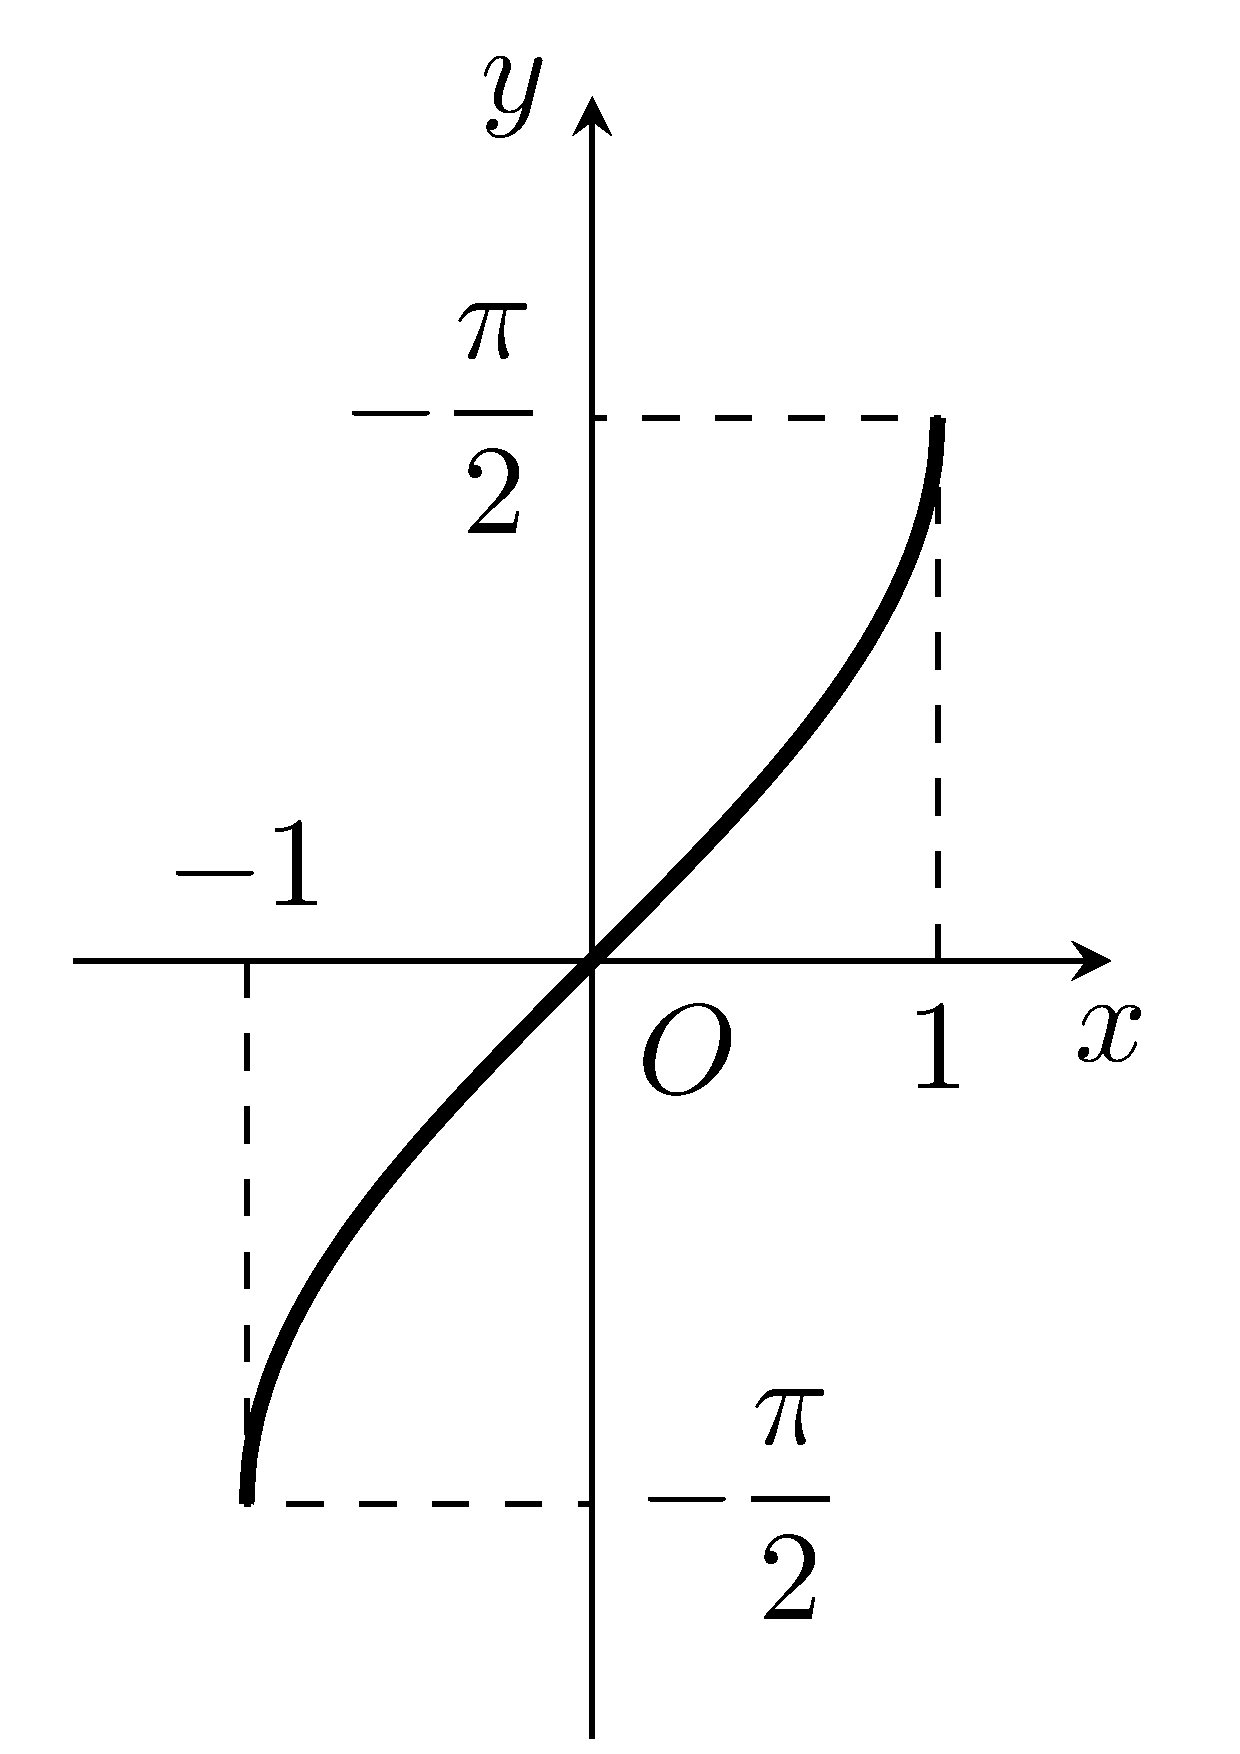
\includegraphics[width=.2\textwidth]{fig/fig1.pdf} &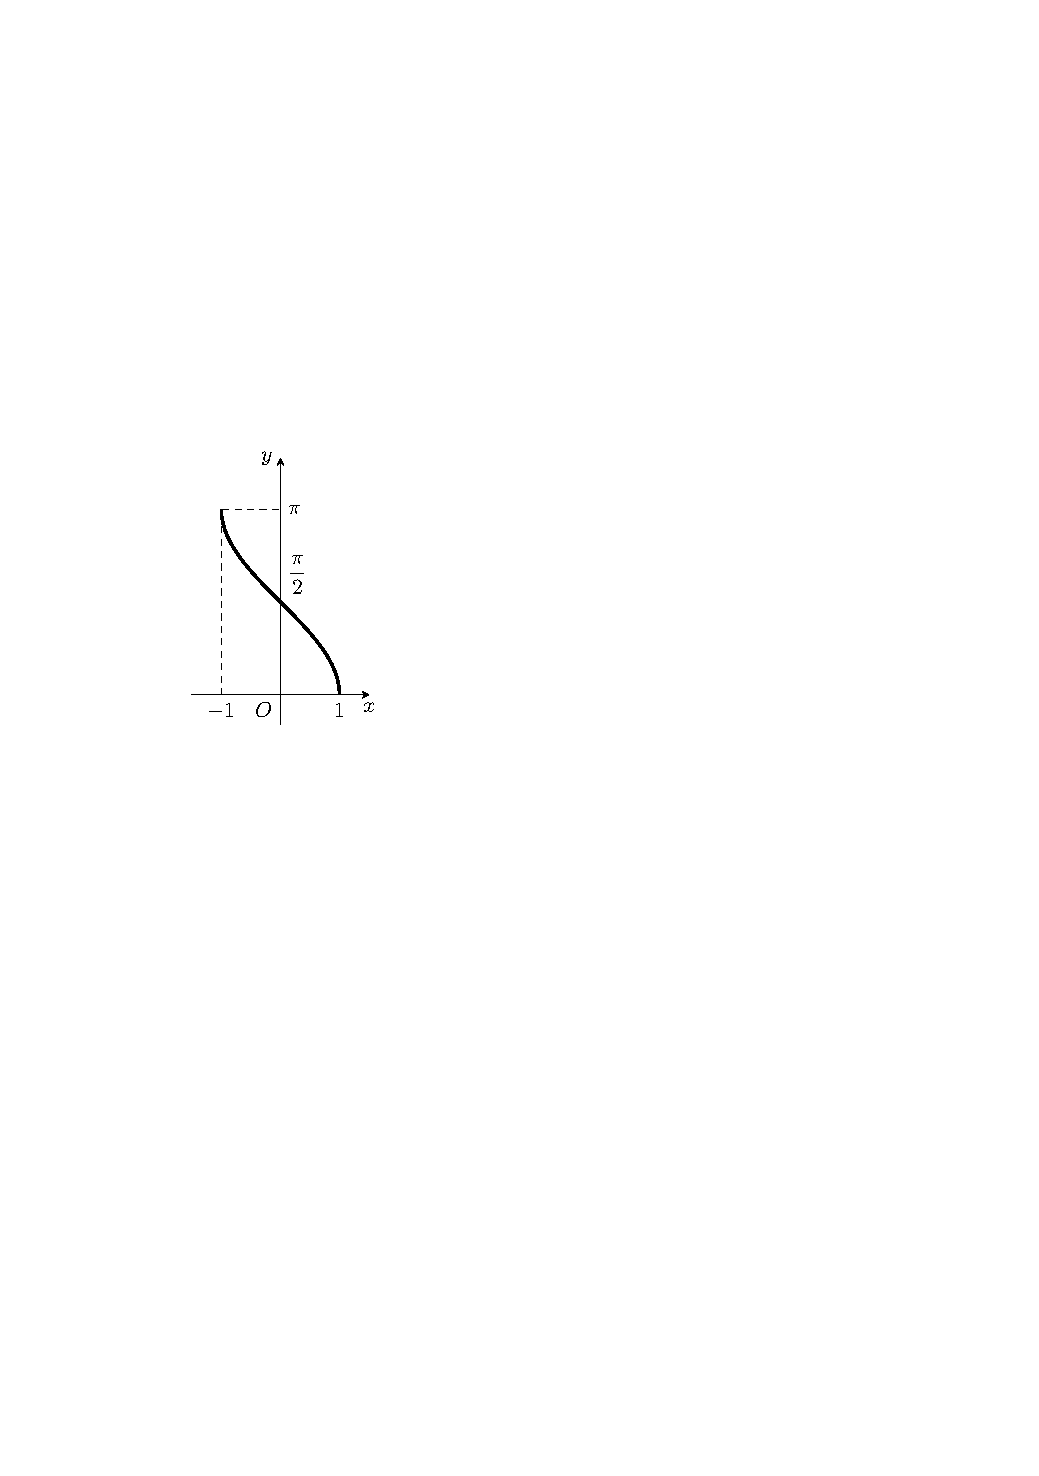
\includegraphics[width=.2\textwidth]{fig/fig2.pdf}&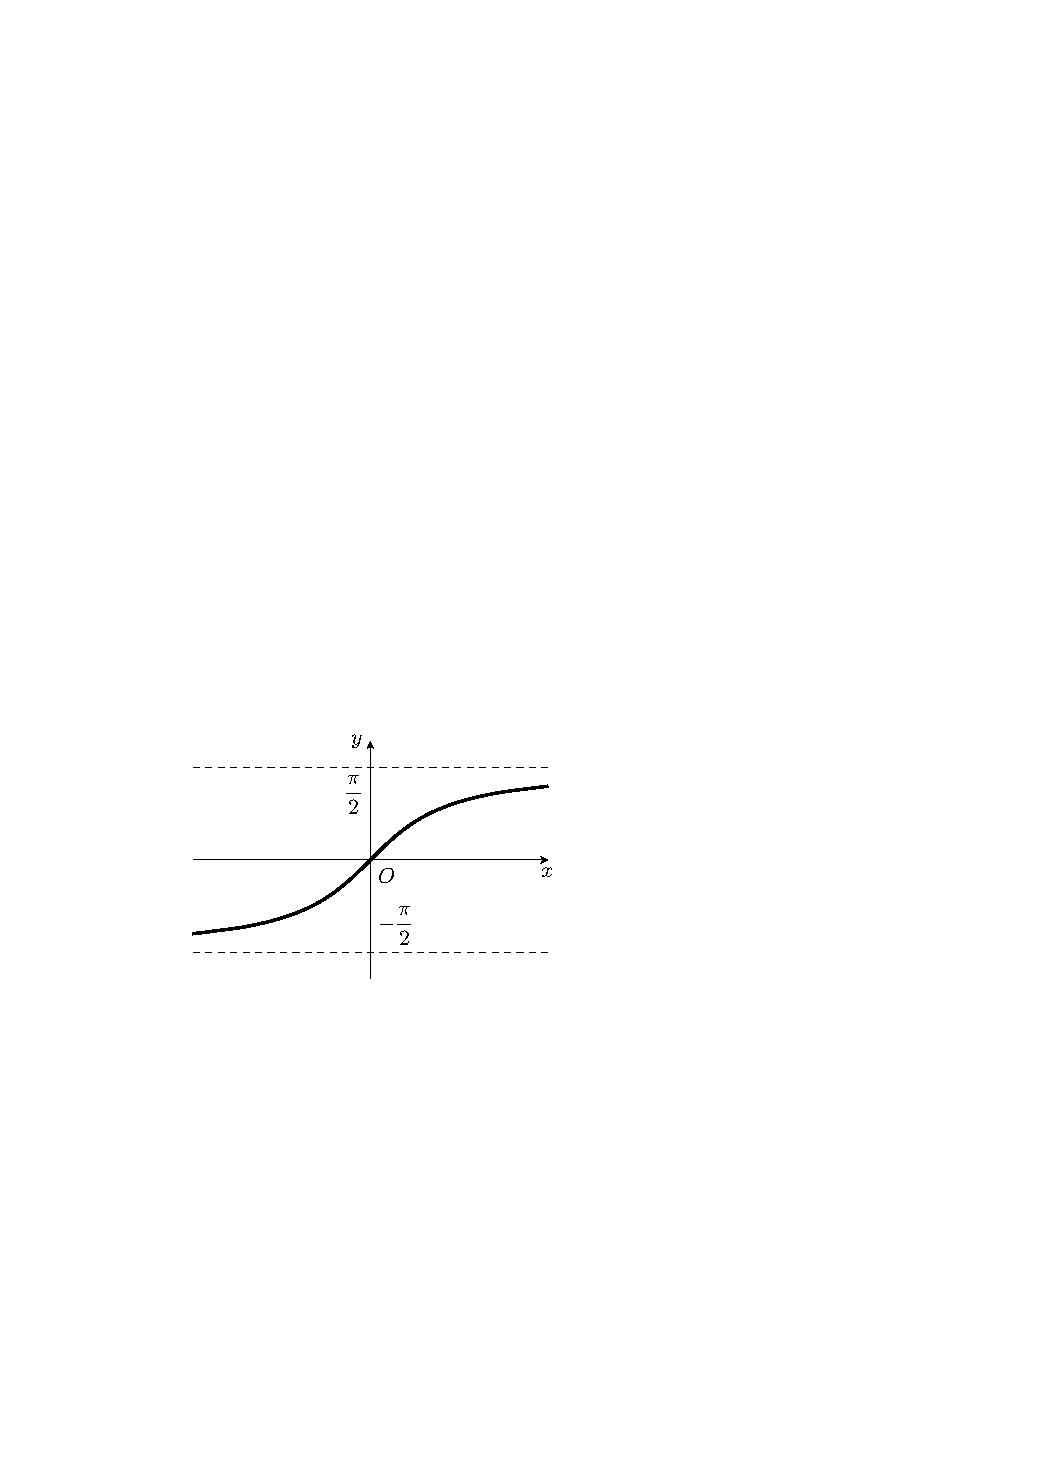
\includegraphics[width=.3\textwidth]{fig/fig3.pdf}&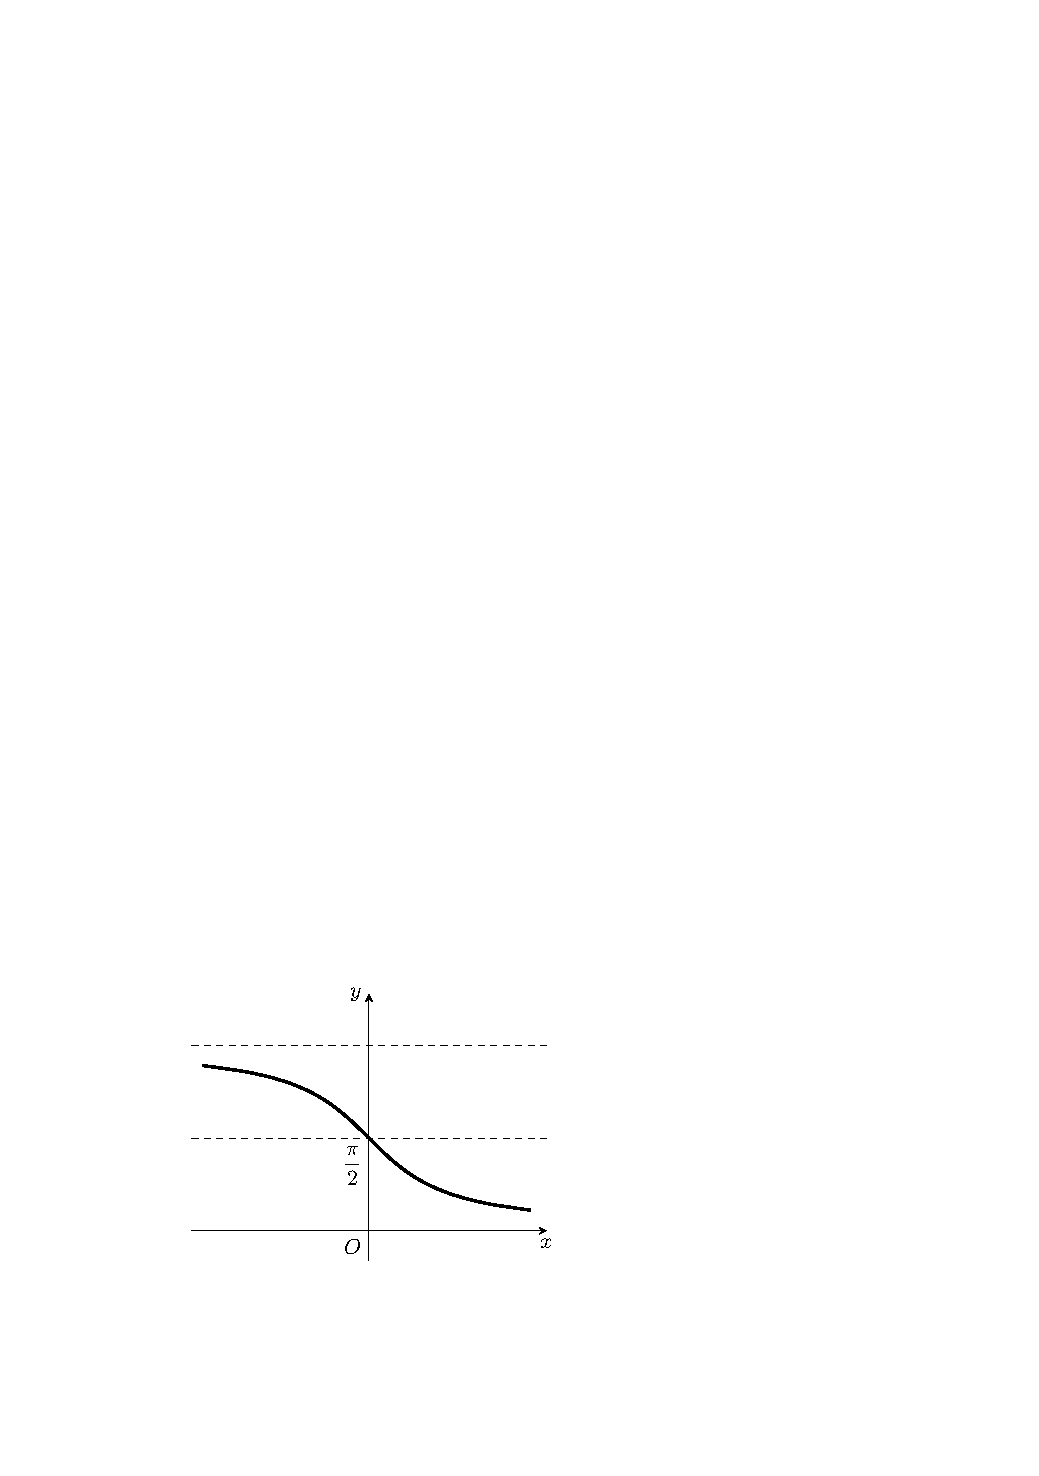
\includegraphics[width=.3\textwidth]{fig/fig4.pdf}\\ 
对应&$\sin(\arcsin x)=x$&$\cos(\arccos x)=x$&$\tan(\arctan x)=x$&$\cot(\arccot x)=x$\\
法则&$(|x|\le 1)$&$(|x|\le 1)$\\
基本& $\arcsin(\sin x)=x$& $\arccos(\cos x)=x$& $\arctan(\tan x)=x$& $\arccot(\cot x)=x$\\
公式&$\left(|x|\le \frac{\pi}{2}\right)$& $(0\le x\le \pi)$ &$\left(|x|<\frac{\pi}{2}\right)$&$(0<x<\pi)$\\ 
奇偶性&奇函数 &非奇非偶& 奇函数&非奇非偶\\
&$\arcsin(-x)=-\arcsin x$&$\arccos(-x)=\pi-\arccos x$&$\arctan(-x)=-\arctan x$&$\arccot(-x)=\pi-\arccot x$\\
&$(|x|\le 1)$&$(|x|\le 1)$\\ 
单调性& 增函数&减函数& 增函数&减函数\\  
基本公式&\multicolumn{2}{c}{$\arcsin x+\arccos x=\frac{\pi}{2},\quad (|x|\le 1)$}&\multicolumn{2}{c}{$\arctan x+\arccot x=\frac{\pi}{2}$}\\
\hline
\end{tabular}
\end{landscape}
















































































































































\subsection{几点说明}
\begin{enumerate}
\item 反三角函数的建立及注意的问题:

由于确定四个三角函数的映射不是一一映射,所以它们都不存在反函数。我们以三角函数为原型,取它们定义域的子集及其映射,这时它们的映射是一一映射,存在反函数。由此,我们分别定义了四个反三角函数。正因此,我们在研究有关反三角函数的问题时,特别要注意自变量的取值范围。
\item 研究反三角函数的一般方法:

研究反三角函数的性质时,要数形结合,充分利用反三角函数的图象;有时利用三角函数线也是比较 直观和方便的。在解决有关反三角函数的问题时,把问题转化为三角函数的问题,是基本的方法。
\end{enumerate}

\section*{复习题四}

\begin{center}
\bfseries A
\end{center}

\begin{enumerate}
    \item 求下列函数的反函数,并写出反函数的定义域、值域:
\begin{multicols}{2}
\begin{enumerate}[(1)]
    \item $y=2\arccos\frac{x}{4}$
    \item $y=\frac{\pi}{2}+\arctan 2x$
    \item $y=\sin x\quad \left(\frac{\pi}{2}\le x\le \frac{3\pi}{2}\right)$
    \item $y=\cos x\quad \left(-\frac{\pi}{2}\le x\le 0\right)$
\end{enumerate}
\end{multicols}

\item 比较下列各组中两实数的大小:
\begin{multicols}{2}
\begin{enumerate}[(1)]
    \item $\arccos\left(-\frac{7}{8}\right)$与$\arccos\left(-\frac{6}{7}\right)$
    \item $\arctan\left(-3\right)$与$\arctan\left(-5\right)$
    \item $\arcsin\left(\cos 4\right)$与$\arcsin\left(\cos 6\right)$
    \item $\arccot\left(\tan 6\right)$与$\arccot\left(\tan {7}\right)$
\end{enumerate}
\end{multicols}

\item 用反三角中的锐角把下列各式中的$x$表示出来。
\begin{multicols}{2}
\begin{enumerate}[(1)]
    \item $\sin x=-\frac{1}{4}\quad \left(-\frac{\pi}{4}<x<0\right)$
    \item $\sin x=\frac{3}{5}\quad \left(\frac{\pi}{2}<x<\pi\right)$
    \item $\cos x-\frac{3}{7}=0\quad \left(-\frac{\pi}{2}<x<0\right)$
    \item $\cos x=\frac{2}{3}\quad \left(2\pi<x<3\pi\right)$
    \item $\tan x+\sqrt{5}=0\quad \left(\frac{\pi}{2}<x<\pi\right)$
    \item $3\cot x+1=0\quad \left(0<x<\pi\right)$
\end{enumerate}
\end{multicols}

\item 求下列各式的值:
\begin{multicols}{2}
\begin{enumerate}[(1)]
    \item $\sin\left(2\arcsin \frac{1}{4}\right)$
    \item $\cos\left[\frac{1}{2}\arcsin \left(-\frac{4}{5}\right)\right]$
    \item $\cos\left(\arccos\frac{3}{5}-\arcsin\frac{5}{13} \right)$
    \item $\tan\left(\arcsin \frac{3}{5}-\arccos\frac{1}{2}\right)$
\end{enumerate}
\end{multicols}

\item 求下列各式中的$x$:
\begin{multicols}{2}
\begin{enumerate}[(1)]
    \item $\arcsin\frac{20}{29}=\arccos x$
    \item $\arcsin x=\arccos\frac{5}{12}$
    \item $\arccot\frac{11}{60}+\arctan x=0$
\end{enumerate}
\end{multicols}

\item 求下列各式的值:
\begin{multicols}{2}
\begin{enumerate}[(1)]
\item $\arcsin\frac{4}{5}+\arcsin\frac{3}{5}$
\item $\arccos\frac{1}{3}+\arccos\left(-\frac{1}{3}\right)$
\item $\arccot\frac{4}{7}+\arccot \frac{3}{11}$
\item $\arctan\sqrt{3}+\arctan\sqrt{2}$
\end{enumerate}
\end{multicols}

\item 求证下列各式:
\begin{enumerate}[(1)]
    \item $\arcsin x+\arccos x=\frac{\pi}{2}\quad (|x|\le 1)$
    \item $\arctan 1+\arctan 2+\arctan 3=\pi$
\end{enumerate}

\item 已知等腰三角形的高与底的比为$4:3$,用反三角函数把它的三个内角表示出来。
\item 若$m$、$n$为方程$6x^2-5x+1=0$的两个根,

证明:$\arctan m+\arctan n=\frac{\pi}{4}$
\end{enumerate}


\begin{center}
    \bfseries B
\end{center}

\begin{enumerate}\setcounter{enumi}{9}
    \item 求下列函数的定义域、值域:
\begin{multicols}{2}
\begin{enumerate}[(1)]
    \item $y=\frac{1}{\arccos x}$
    \item $y=\arctan\sqrt{x}$
    \item $y=\sqrt{\arctan x}$
    \item $y=\sqrt{\arccot(2x-5)}$
    \item $y=\sqrt{\arcsin\frac{1}{x}}$
    \item $y=\arccos(x^2+x)$
    \item $y=\arccos(\arcsin x)$
    \item $y=\log_a\left(\arccos x-\frac{\pi}{3}\right)$
\end{enumerate}
\end{multicols}


\item 判断函数$y=\arccos x-\frac{\pi}{2}$的奇偶性。
\item 求满足下列不等式的$x$的取值范围;
\begin{multicols}{2}
\begin{enumerate}[(1)]
    \item $\arcsin (-x)<\arcsin x$
    \item $\arccos x<\arccos (1-x)$
\end{enumerate}
\end{multicols}

\end{enumerate}



 \chapter{三角方程}
先看下面的实例。

若$E$是$\angle BAC$的角平分线上的一个定点,已知$\angle BAC=60^{\circ}$(图5.1),过$E$点的动直线$BC$交
$\angle BAC$的两边于$B$、$C$. 试问当直线$BC$绕点$E$旋转到什么位置时,$AB=2AC$?

\noindent
\begin{minipage}{.45\textwidth}
\begin{analyze}
当直线旋转时(我们可以用旋转角$x$来刻画这个旋转),$\triangle BAC$是个可变图形。欲使$AB=2AC$,应设法分别找出边$AB$、$AC$与变量$x$的函数关系(这本质上是一个解斜三角形的问题),然后用方程的方法解之.
\end{analyze}
\end{minipage}
\hfill
\begin{minipage}{.45\textwidth}
\centering
\begin{tikzpicture}[scale=.7]
\tkzDefPoints{0/0/A, 4/0/E, 6/0/F}
\tkzDefPoint(-35:3.5){C}
\tkzDefPoint(25:7){B'}
\tkzInterLL(A,B')(C,E)
\tkzGetPoint{B}
\tkzLabelPoints[left](A)
\tkzLabelPoints[below](C,E)
\tkzLabelPoints[above](B)
\draw(B')--(A)--(F);
\tkzDrawPolygon(A,C,B)
\node at (2,0)[below]{$m$};
\tkzMarkAngles[mark=none, size=.8cm](C,A,E F,E,B)
\tkzMarkAngles[mark=none, size=1cm](E,A,B)
\tkzMarkAngles[mark=none, size=.6cm](B,E,A)
\tkzLabelAngle[pos=1.2](F,E,B){$x$}
\tkzLabelAngle[pos=1.1](B,E,A){$180^{\circ}-x$}

\end{tikzpicture}
    \captionof{figure}{}
\end{minipage}

\begin{solution}
由于$E$是$\angle BAC$的角平分线上的定点,故可用字母$m$表示$AE$的长。容易看出$\triangle ABE$是可解的:$\angle BAE=30^{\circ}$, $\angle B=x-30^{\circ}$, $\angle AEB=180^{\circ}-x$,$AE=m$,由正弦定理,得
\[\begin{split}
    \frac{AB}{\sin(180^{\circ}-x)}&=\frac{m}{\sin(x-30^{\circ})}\\
    AB&=\frac{m\sin x}{\sin (x-30^{\circ})}
\end{split}\]
同理,可得:$AC=\frac{m\sin x}{\sin(x+30^{\circ})}$.

欲使$AB=2AC$,应使
\[2m\sin x\sin (x-30^{\circ})=m\sin x\sin(x+30^{\circ})\]
显然$m\sin x\ne 0$,上式可简化为
\[2\sin (x-30^{\circ})=\sin(x+30^{\circ})\]
\end{solution}

这种三角函数符号中含有未知数的等式称为\textbf{三角方程},又如
\[\sin x=\frac{1}{3},\quad \tan^2 x-5\tan x-3=0,\quad 3\cos\frac{x}{2}+\cos x-1=0\]
\[\frac{1+\tan x}{1-\tan x}=1+\sin2x,\quad a\sin x+b\cos x=c,\quad \sin^{100}x+8\sin^5x-2=0\]
等都是三角方程。它们来自数学、物理和技术工程。

本章将研究一些简单三角方程的求解问题。

\section{最简三角方程}
在三角方程中,$\sin x=a$, $\cos x=a$, $\tan x=a$, $\cot x=a$是最简单的(称为\textbf{最简三角方程}),也是最基本的最重要的。其他三角方程的求解,往往是归结为这四种最简三角方程的求解。


\subsection{方程$\sin x=a$的解集}

方程的解集自然依赖于常数$a$的取值和对变元$x$的限定范围。对于后者,若不附任何条件,就意味着是在$(-\infty,+\infty)$上求方程的解集(下同).
\begin{enumerate}[(1)]
    \item 当$|a|>1$时,由于任取$x\in\R$,都有$|\sin x|\le 1$
    
    $\therefore\quad$ 方程无解,即解集为$\emptyset$.
    \item 当$|a|\le 1$时,我们先求出方程的特解(图5.2):
\[\alpha_1=\arcsin a,\qquad \alpha_2=\pi-\arcsin a\]
\begin{figure}[htp]
    \centering
\begin{tikzpicture}[>=stealth]
\begin{scope}
\draw[->](-2.5,0)--(2.5,0)node[below]{$x$};
\draw[->](0,-2)--(0,2.5)node[left]{$y$};
\draw(0,0)node[below right]{$O$} circle (1.5);
\draw[very thick](180-45:1.5)node[above left]{$P_2$}--(0,0)--(45:1.5)node[above right]{$P_1$};
\draw[dashed](180-45:1.5)--(45:1.5);
\draw[thick, ->](0,0)--node[right]{$a$}(0,.75*1.414)node[above left]{$M$};
\draw[->](.5,0) arc (0:45:.5)node[right]{$\alpha_1$};
\draw[->](.35,0) arc (0:135:.35)node[above]{$\alpha_2$};
\node at (1.5,0)[above right]{$A$};
\node at (0,1.5)[above right]{$B$};
\node at (1.5,0)[below right]{$1$};
\end{scope}
\begin{scope}[xshift=6cm]
\draw[->](-2.5,0)--(2.5,0)node[below]{$x$};
\draw[->](0,-2)--(0,2.5)node[left]{$y$};
\draw(0,0)node[above right]{$O$} circle (1.5);
\node at (1.5,0)[below right]{$1$};
\draw[very thick](-135:1.5)node[below left]{$P_1$}--(0,0)--(-45:1.5)node[below right]{$P_2$};
\draw[dashed](-135:1.5)--(-45:1.5);
\draw[thick, ->](0,0)--node[right]{$a$}(0,-.75*1.414)node[below right]{$M$};
\draw[->](.5,0) arc (0:-45:.5)node[right]{$\alpha_1$};
\draw[->](.75,0) arc (0:180+45:.75);
\node at (115:1){$\alpha_2$};

\end{scope}    
\end{tikzpicture}
    \caption{}
\end{figure}
然后,再加上“周期的整数倍”即得到方程的\textbf{通解}:
\[\begin{split}
    x_1&=\arcsin a+2k\pi,\\
    x_2&=(\pi-\arcsin a)+2k\pi,
\end{split}\quad k\in\Z\]
$x_1,x_2$的表达式有时合并写成
\[x=k\pi+(-1)^k\arcsin a,\quad k\in\Z\]
即方程的解集为
\begin{equation}
    \left\{x\mid x=k\pi+(-1)^k\arcsin a,\; k\in\Z\right\}\tag{*}
\end{equation}
\end{enumerate}

应注意:(*)是在$|a|\le 1$时的解集,若忘掉$|a|\le 1$这个条件,说$\sin x=a$的解集是(*),那就不正确.

\subsection{方程$\cos x=a$的解集}
\begin{enumerate}
    \item 当$|a|>1$时,$\cos x=a$的解集为$\emptyset$;
    \item 当$|a|\le 1$时,$\cos x=a$的特解为(图5.3)
\[\alpha_1=\arccos a,\qquad \alpha_2=-\arccos a\]
\begin{figure}[htp]
    \centering
\begin{tikzpicture}[>=stealth]
\begin{scope}
\draw[->](-2.5,0)--(2.5,0)node[below]{$x$};
\draw[->](0,-2)--(0,2.5)node[left]{$y$};
\draw(0,0)node[below left]{$O$} circle (1.5);
\draw[very thick](45:1.5)node[above right]{$P_1$}--(0,0)--(-45:1.5)node[below right]{$P_2$};
\draw[dashed](-45:1.5)--(45:1.5);
\draw[thick, ->](0,0)--(.75*1.414,0)node[above]{$N$};
\node at (.75*1.3,0)[below]{$a$};
\draw[->](.35,0) arc (0:45:.35)node[right]{$\alpha_1$};
\draw[->](.45,0) arc (0:-45:.45)node[right]{$\alpha_2$};
\node at (1.5,0)[above right]{$A$};
\node at (-1.5,0)[above left]{$B$};
\node at (1.5,0)[below right]{$1$};
\end{scope}
\begin{scope}[xshift=6cm]
\draw[->](-2.5,0)--(2.5,0)node[below]{$x$};
\draw[->](0,-2)--(0,2.5)node[left]{$y$};
\draw(0,0)node[below right]{$O$} circle (1.5);
\node at (1.5,0)[above right]{$A$};
\node at (1.5,0)[below right]{$1$};
\draw[very thick](-135:1.5)node[below left]{$P_2$}--(0,0)--(135:1.5)node[above left]{$P_1$};
\draw[dashed](-135:1.5)--(135:1.5);
\draw[thick, ->](0,0)--node[below]{$a$}(-.75*1.414,0)node[above]{$N$};
\draw[->](.5,0) arc (0:135:.5);
\draw[->](.75,0) arc (0:-135:.75);
\node at (-66:1){$\alpha_2$};
\node at (-1.5,0)[above left]{$B$};
\node at (66:.7){$\alpha_1$};
\end{scope}    
\end{tikzpicture}
    \caption{}
\end{figure}


通解为
\[\begin{cases}
    x_1=\arccos a+2k\pi\\
    x_2=-\arccos a+2k\pi
\end{cases} \mathop{\Longleftrightarrow}^{\text{合并为}} x=2k\pi\pm \arccos a,\quad k\in\Z\]
写成解集的形式为
\[\left\{x\mid x=2k\pi\pm\arccos a,\; k\in\Z\right\}\]
\end{enumerate}

\subsection{方程$\tan x=a$的解集}
由于$\tan x$的值域为$(-\infty,+\infty)$,所以对任意$a\in\R$,方程都有解。其特解为(图5.4)
\[\alpha_1=\arctan a,\qquad \alpha_2=\arctan a+\pi\]
其通解为
\[\begin{cases}
    x_1=\arctan a+2k\pi\\
    x_2=(\arctan a+\pi)+2k\pi    
\end{cases}\mathop{\Longleftrightarrow}^{\text{合并为}} x=\arctan a+k\pi,\; k\in\Z  \]
写成解集的形式为$\{x\mid x=\arctan a+k\pi,\; k\in\Z\}$.
\begin{figure}[htp]
    \centering
\begin{tikzpicture}[>=stealth]
\begin{scope}
\draw[->](-2.5,0)--(2.5,0)node[below]{$x$};
\draw[->](0,-2.5)--(0,2.5)node[left]{$y$};
\draw(0,0)node[below right]{$O$} circle (1.5);
\draw(1.5,3)--(1.5,-2);
\draw[dashed](-120:1.5)node[below left]{$P_2$}--(60:1.5)node[above]{$P_1$}--(60:3)node[right]{$T$};
\node at (1.5,0)[above right]{$A$};
\node at (1.5,0)[below right]{$1$};
\draw[thick,->](1.5,0)--node[right]{$a$}(60:3);
\draw[->](.5,0) arc (0:180+60:.5)node[above left]{$\alpha_2$};
\draw[->](.7,0) arc (0:60:.7)node[right]{$\alpha_1$};

\end{scope}
\begin{scope}[xshift=6cm]
    \draw[->](-2.5,0)--(2.5,0)node[below]{$x$};
    \draw[->](0,-2.5)--(0,2.5)node[left]{$y$};
    \draw(0,0)node[below left]{$O$} circle (1.5);
    \draw(1.5,2)--(1.5,-3);
    \node at (1.5,0)[above right]{$A$};
    \node at (1.5,0)[below right]{$1$};
    \draw[dashed](120:1.5)node[above left]{$P_2$}--(-60:1.5)node[below]{$P_1$}--(-60:3)node[right]{$T$};
    \draw[thick,->](1.5,0)--node[right]{$a$}(-60:3);
    \draw[->](.5,0) arc (0:120:.5)node[above right]{$\alpha_2$};
    \draw[->](.7,0) arc (0:-60:.7)node[right]{$\alpha_1$};
\end{scope}    
\end{tikzpicture}
    \caption{}
\end{figure}

\subsection{方程$\cot x=a $的解集}

$\cot x$的值域也是$(-\infty,+\infty)$,所以任意$a\in\R$,方程都有解,其特解为(图5.5)
\[\alpha_1=\arccot a,\qquad \alpha_2=\arccot a+\pi\]
其通解为
\[\begin{cases}
    x_1=\arccot a+2k\pi\\
    x_2=(\arccot a+\pi)+2k\pi    
\end{cases}\mathop{\Longleftrightarrow}^{\text{合并为}} x=\arccot a+k\pi,\; k\in\Z  \]
写成解集的形式为$\{x\mid x=\arccot a+k\pi,\; k\in\Z\}$.

\begin{figure}[htp]
    \centering
\begin{tikzpicture}[>=stealth]
\begin{scope}
\draw[->](-2.5,0)--(2.5,0)node[below]{$x$};
\draw[->](0,-2)--(0,2.5)node[left]{$y$};
\draw(0,0)node[below right]{$O$} circle (1.5);
\draw[thick, ->](0,1.5)node[above right]{$B$}--node[above]{$a$}(1.2*1.5,1.5)node[right]{$G$};
\draw[dashed](180+40:1.5)node[below left]{$P_2$}--(1.2*1.5,1.5);
\node at (40:1.5)[right]{$P_1$};
\node at (1.5,0)[above right]{$A$};

\draw[->](.5,0) arc (0:180+40:.5)node[above left]{$\alpha_2$};
\draw[->](.7,0) arc (0:40:.7)node[right]{$\alpha_1$};

\end{scope}
\begin{scope}[xshift=6cm]
    \draw[->](-2.5,0)--(2.5,0)node[below]{$x$};
    \draw[->](0,-2)--(0,2.5)node[left]{$y$};
    \draw(0,0)node[above right]{$O$} circle (1.5);
    \draw[thick, ->](0,1.5)node[above right]{$B$}--node[above]{$a$}(-1.2*1.5,1.5)node[above]{$G$};
    \draw[dashed](-40:1.5)node[below right]{$P_2$}--(-1.2*1.5,1.5);
    \node at (180-40:1.5)[left]{$P_1$};
    \node at (1.5,0)[above right]{$A$};
    \node at (1.5,0)[below right]{$1$};
    \draw[->](.5,0) arc (0:270+50:.5);
    \draw[->](.7,0) arc (0:180-40:.7);
    \node at (70:1){$\alpha_1$};
    \node at (-120:.8){$\alpha_2$};

\end{scope}    
\end{tikzpicture}
    \caption{}
\end{figure}

\begin{example}
    解方程:
\begin{multicols}{3}
\begin{enumerate}[(1)]
    \item $2\sin x+\sqrt{2}=0$
    \item $2\cos 2x=1$
    \item $\tan(x+15^{\circ})+1=0$
\end{enumerate}
\end{multicols}
\end{example}

\begin{solution}
\begin{enumerate}
    \item $2\sin x+\sqrt{2}=0\Longleftrightarrow \sin x=-\frac{\sqrt{2}}{2}$
\[\begin{split}
    \therefore\quad x_1&=\arcsin\left(-\frac{\sqrt{2}}{2}\right)+2k\pi=-\frac{\pi}{4}+2k\pi\\
    x_2&=\pi-\arcsin\left(-\frac{\sqrt{2}}{2}\right)+2k\pi=\frac{5\pi}{4}+2k\pi\\
\end{split}\qquad (k\in\Z)\]
写成解集\footnote{求方程解集的过程叫解方程. 为了书写简便,也可以只列出所有的解而不必写成集合形式.}为
\[\left\{x\mid x=-\frac{\pi}{4}+2k\pi \text{ 或 } x=\frac{5\pi}{4}+_2k\pi,\; k\in\Z\right\}\]

\item $2\cos 2x=1\Longleftrightarrow \cos 2x=\frac{1}{2}$

$\therefore\quad 2x=2k\pi\pm \arccos\frac{1}{2} \quad \Rightarrow\quad x=k\pi\pm\frac{\pi}{6}\quad (k\in\Z) $

写成解集为$\left\{x\mid x=k\pi\pm \frac{\pi}{6},\; k\in\Z\right\}$

\begin{rmk}
下面的解法是错误的:
\[2x=\pm \arccos\frac{1}{2},\qquad x=\pm\frac{1}{2} \arccos \frac{1}{2}\]
$\therefore\quad x=2k\pi\pm \frac{1}{2} \arccos \frac{1}{2}\quad (k\in\Z)$.
\end{rmk}


\item $\tan(x+15^{\circ})+1=0 \Longleftrightarrow \tan (x+15^{\circ})=-1$,

$\therefore\quad (x+15^{\circ})=\arctan(-1)+k\cdot 180^{\circ}=-45^{\circ}+180^{\circ}\cdot k$

$\therefore\quad x=-60^{\circ}+180^{\circ}\cdot k\quad (k\in\Z)$.

写成解集为$\{x\mid x=-60^{\circ}+180^{\circ}\cdot k,\;  k\in\Z\}$。

\begin{rmk}
    在同一个表达式中应使用相同的单位。
    
    如上面的式子不能写成$x+15^{\circ}=-\frac{\pi}{4}+k\pi\; (k\in\Z)$的形式。
\end{rmk}
\end{enumerate}
\end{solution}


\begin{example}
    若$0^{\circ}<x<360^{\circ}$,解方程$\sin(3x-105^{\circ})=-\frac{1}{2}$.
\end{example}

\begin{solution}
\[\begin{split}
\because\quad &(3x_1-105^{\circ})=\arcsin\frac{1}{2}+360^{\circ}\cdot k=30^{\circ}+360^{\circ}\cdot k\quad (k\in\Z)   \\
&(3x_2-105^{\circ})=180^{\circ}-\arcsin\frac{1}{2}+360^{\circ}\cdot k=150^{\circ}+360^{\circ}\cdot k\quad (k\in\Z)   
\end{split}\]

$\therefore\quad x_1=45^{\circ}+120\cdot k,\qquad x_2=85^{\circ}+120^{\circ}\cdot k\quad (k\in\Z)$

考虑到$0^{\circ}<x<360^{\circ}$,
\begin{enumerate}
    \item 在$x_1$中令$k=0,1,2$,得$45^{\circ},\; 165^{\circ},\; 285^{\circ}$;
    \item 在$x_2$中令$k=0,1,2$,得$85^{\circ},\; 205^{\circ},\; 325^{\circ}$.
\end{enumerate}

$\therefore\quad $原方程的解集为$\{45^{\circ},\; 165^{\circ},\; 285^{\circ},\; 85^{\circ},\; 205^{\circ},\; 325^{\circ}\}$.
\end{solution}

\section*{习题一}
\begin{center}
    \bfseries A
\end{center}
\begin{enumerate}
    \item 口答下列方程的解集:
\begin{multicols}{3}
\begin{enumerate}[(1)]
    \item $\sin x=\frac{\sqrt{3}}{2}$
    \item $\sin x=-\frac{1}{2}$
    \item $\cos x=\frac{\sqrt{2}}{2}$
    \item $\cos x=-\frac{1}{2}$
    \item $\tan x=-\sqrt{3}$
    \item $\cot x=\frac{1}{3}$
\end{enumerate}
\end{multicols}
    \item 解下列方程:
  \begin{multicols}{2}
\begin{enumerate}[(1)]
    \item $2\sin2x+1=0$
    \item $\sin\left(\frac{x}{2}+\frac{\pi}{6}\right)=\frac{\sqrt{3}}{2}$
    \item $2\cos\left(\frac{\pi}{3}+45^{\circ}\right)=1$
    \item $\tan 2x-\sqrt{3}=0$
    \item $\frac{1}{2}\cot 2(x+25^{\circ})-2=0$
    \item $3\tan\frac{x+20^{\circ}}{3}=\sqrt{3}$ 
    
$(-1000^{\circ}<x<1000^{\circ})$
\end{enumerate}
\end{multicols}
\end{enumerate}

\section{简单三角方程}
一些简单的三角方程,可以通过三角函数的恒等变形或代数方法,化归上节研究过的四种最简三角方程,从而获得其解。现举几类,着重说明“化归”的思路和方法,悟出了道理,可见一般。

\subsection{同角同名的三角函数方程}
\begin{example}
   解下列方程: 
\begin{multicols}{2}
\begin{enumerate}[(1)]
    \item $2\sin^2 x-5\sin x-3=0$
    \item $\sin^2 x-\cos^2 x=\cos x$
    \item $3\cos\frac{x}{2}+\cos x=1$
    \item $\frac{1+\tan x}{1-\tan x}=1+\sin 2x$
\end{enumerate}
\end{multicols}
\end{example}

\begin{analyze}
把新问题化归为已研究过的问题,是数学研究中的通法。对于(1),实行换元,即令$\sin x=y$,可得到关于$y$的一元二次方程,从而可以解出$y$,这就化归为最简 三角方程的第一种。其余几题,只须稍作三角函数变换,就可以实现化归。
\end{analyze}

\begin{solution}
\begin{enumerate}[(1)]
    \item 令$y=\sin x\; (-1\le y\le 1)$,有$2y^2-5y-3=0$,即$$(y-3)(2y+1)=0\Rightarrow y_1=3,\; y_2=\frac{-1}{2}$$

$\therefore\quad \sin x=3$(无解);$\sin x=\frac{-1}{2}$ 解之,得
\[x_1=\frac{-\pi}{6}+2k\pi,\quad x_2=\frac{7\pi}{6}+2k\pi,\; k\in\Z\]
\item 把$\sin x$化为$\cos x$,得
\[2\cos^2x+\cos x-1=0\]
令$\cos x=y\; (-1\le y\le 1)$,有$2y^2+y-2=0$,
即$$(y+1)(2y-1)=0\Longleftrightarrow y_1=-1,\quad y_2=\frac{1}{2}$$
\[\begin{split}
    \therefore\quad \cos x=-1 &\Longleftrightarrow x_1=\pi+2k\pi \; (k\in\Z)\\
    \cos x=\frac{1}{2}&\Longleftrightarrow x_2=2k\pi \pm \frac{\pi}{3}\; (k\in\Z)
\end{split}\]
\item 把$\cos x$写成 $2\cos^2\frac x2-1$, 可得
$$2\cos ^{2}\frac x2+ 3\cos \frac x2- 2= 0$$
令$y=\cos\frac{x}{2}\quad (-1\leqslant y\leqslant1)$, 有
$$2y^{2}+ 3y- 2= 0\Longleftrightarrow y_{1}= - 2,\quad y_{2}= \frac 12$$
即 $\cos \frac x2= - 2$ (无解),\quad $\cos\frac x2=\frac12$

$\therefore\quad \frac x2= 2k\pi \pm$ $\frac \pi 3\left ( k\in Z\right ) \Longleftrightarrow x= 4k\pi \pm \frac {2\pi }3\left ( k\in Z\right ) $

\item 把$\sin2x$写成$\frac{2\tan x}{1+\tan ^{2}x}$, 有$\frac {1+ \tan x}{1- \tan x}= 1+ \frac {2\tan x}{1+ \tan ^{2}x}$,

令 $y= \tan x$, 有
\[\begin{split}
    \frac {1+ y}{1- y}- 1= \frac {2y}{1+ y^{2}}&\Longleftrightarrow \frac {2y}{1- y}- \frac {2y}{1+ y^{2}}= 0\\
    &\Longleftrightarrow 2y\left(\frac{1}{1-y}-\frac{1}{1+y^{2}}\right)=0\\
    &\Longleftrightarrow 2y\cdot\frac{y(y+1)}{(1+y^{2})(1-y)}=0\\
    &\Longleftrightarrow y_{1}= 0,\quad y_{2}= - 1
\end{split}\]
即 
\[\begin{split}
    \tan x= 0&\Longleftrightarrow x_1= k\pi\quad ( k\in \Z) \\
    \tan x= -1&\Longleftrightarrow x_{2}= - \frac \pi 4+ k\pi\quad ( k\in \Z) 
\end{split}\]
\end{enumerate}
\end{solution}

\begin{remark}
    此例的特点和化归方法可以简捷地概括为“同角同名(包括可化为同角同名函数的方程)——换元就行”。此例中,每小题都列出了所有的解,而未写成解集的形式。
\end{remark}

\subsection{两同名函数相等的方程}

这类方程的一般形式为
\begin{align}
    \sin f(x)&=\sin g(x) \tag{1}\\
    \cos f(x)&=\cos g(x) \tag{2}\\
    \tan f(x)&=\tan g(x) \tag{3}\\
    \cot f(x)&=\cot g(x) \tag{4}
\end{align}

对于(1),可把$g(x)$看作是$f(x)$的特解(图5.6),有
\[\begin{split}
 f(x)&=g(x)+2k\pi\; (k\in\Z)\longrightarrow \text{解出}x_1\\
f(x)&=\pi-g(x)+2k\pi\; (k\in\Z)\longrightarrow \text{解出}x_2
\end{split}\]
则方程(1)的解集为$\{x\mid x=x_1\text{ 或 }x=x_2\}$;

\noindent
\begin{minipage}{.45\textwidth}
    \centering
\begin{tikzpicture}[>=stealth]
\draw[->](-2.5,0)--(2.5,0)node[below]{$x$} ;   
\draw[->](0,-2)--(0,2.5)node[left]{$y$} ;   
\draw(0,0)node[below right]{$O$} circle (1.5);
\draw[very thick](135:1.5)node[above left]{$\pi-g(x)$}--(0,0)--(45:1.5)node[above right]{$g(x)$};
\draw[dashed](135:1.5)--(45:1.5);
\draw[->](.5,0) arc (0:45:.5);
\draw[->](.35,0) arc (0:135:.35);
\node at (1.5,0)[below right]{$A$};
\end{tikzpicture}    
\captionof{figure}{}
\end{minipage}\hfill
\begin{minipage}{.45\textwidth}
    \centering
\begin{tikzpicture}[>=stealth]
    \draw[->](-2.5,0)--(2.5,0)node[below]{$x$} ;   
\draw[->](0,-2)--(0,2.5)node[left]{$y$} ;   
\draw(0,0)node[below left]{$O$} circle (1.5);
\draw[very thick](-45:1.5)node[below right]{$-g(x)$}--(0,0)--(45:1.5)node[above right]{$g(x)$};
\draw[dashed](-45:1.5)--(45:1.5);
\draw[->](.5,0) arc (0:45:.5);
\draw[->](.35,0) arc (0:-45:.35);
\end{tikzpicture}    
\captionof{figure}{}
\end{minipage}

对于(2),仍然把$g(x)$看作是$f(x)$的特解(图5.7),有
\[ f(x)=2k\pi\pm g(x)\; (k\in\Z)\longrightarrow \text{由此解出}x_1,x_2\]
则方程(2)的解集为$\{x\mid x=x_1\text{ 或 }x=x_2\}$;

同样,对于(3)有$f(x)=g(x)+k\pi\; (k\in\Z)\longrightarrow \text{由此解出}x$;

对于(4)有$f(x)=g(x)+k\pi\; (k\in\Z)\longrightarrow \text{由此解出}x$.

\begin{example}
解方程:
\begin{multicols}{2}
\begin{enumerate}[(1)]
    \item $\tan 4x=\tan 3x$
    \item $\sin4x+\sin2x=0$
\end{enumerate}
\end{multicols}
\end{example}

\begin{solution}
\begin{enumerate}[(1)]
    \item 由$\tan 4x=\tan 3x$得:$4x+3x+k\pi\; (k\in\Z)$

$\therefore\quad x=k\pi\; (k\in\Z)$
\item 由题可得:$\sin 4x=\sin(-2x)$

$\therefore\quad 4x=(-2x)+2k\pi\; (k\in\Z)$,或$4x=\pi-(-2x)+2k\pi\; (k\in\Z)$,有
\[\begin{split}
    6x=2k\pi,&\qquad 2x=\pi+2k\pi\\
x_1=\frac{k\pi}{3}\; (k\in\Z) &\qquad x_2=\frac{\pi}{2}+k\pi \; (k\in\Z)
\end{split}\]

$\therefore\quad $原方程的解集为$\left\{x\mid x=\frac{k\pi}{3}\text{ 或 }x=\frac{\pi}{2}+k\pi,\; k\in\Z\right\}$.
 \end{enumerate}   
\end{solution}

\section*{习题二}
\begin{center}
    \bfseries A
\end{center}

解下列方程:
\begin{enumerate}
    \item $2\sin^{2}x+3\sin x+1=0$
    \item $4\sin^{2}x+(2\sqrt{3}-2)\cos x-(4-\sqrt{3})=0$
\begin{multicols}{2}
    \item $\sec^{2}x=1+\tan x$
    \item $\cos2\theta-\cos3\theta=0$
    \item $\sin3x+\sin4x=0$
    \item $\cot x+\cot3x=0$
    \item $\cos2x+\sin3x=0$
    \item $\sin x=2\sin\left(\frac{\pi}{3}-x\right)$    
\end{multicols}
\end{enumerate}

\subsection{左边化积(分解因式化积或和差化积)右边方程}

从代数上我们知道,方程
$F(x)=f_1(x)\cdot f_2(x)=0$
在函数的定义域$Q$上[不妨把$Q$也称为方程$F(x)=0$的定义域],若$f_1(x)=0$和$f_2(x)=0$的解集分别是$A$与$B$,那么$F(x)
=0$的解集就是$A\cup B$,即
\[F(x)=0,\; x\in Q \Longleftrightarrow f_1(x)=0,\; x\in Q\text{\;与\;}f_2(x)=0,\; x\in Q\]

这里应该特别注意方程$f_1(x)=0$,$f_2(x)=0$是在$Q$上求解,如果忽略了$x\in Q$这个前提,就可能导致错误。


\begin{example}
    解方程:
    \begin{multicols}{2}
\begin{enumerate}[(1)]
    \item $\sin x\cdot \tan x\cdot \cot x=0$
    \item $\sin x\cdot \tan x\cdot \sec x=0$
\end{enumerate}        
    \end{multicols}
\end{example}

\begin{solution}
\begin{enumerate}[(1)]
    \item 方程的定义域为$Q:x\in\R$,且$x\ne \frac{\pi}{2}+k\pi,\; x\ne k\pi\; (k\in\Z)$。显然,在$Q$上$\sin x\ne 0$,$\tan x\ne 0$,$\cot x\ne 0$
    
    $\therefore\quad $原方程无解(或说解集为$\emptyset$)。
\item 方程的定义域为$Q:x\in\R$,且$x\ne \frac{\pi}{2}+k\pi\; (k\in\Z)$。
\[\begin{split}
    \therefore\quad \sin x=0\; (x\in Q)&\Longleftrightarrow x_1=k\pi\; (k\in\Z)\\
    \tan x=0\; (x\in Q)&\Longleftrightarrow x_2=k\pi\; (k\in\Z)\\
  \sec  x=0\; (x\in Q)&\Longleftrightarrow  \frac{1}{\cos x}=0\; (x\in Q) \Longleftrightarrow x\in\emptyset\\
\end{split}\]
\end{enumerate}

$\therefore\quad $原方程的解为$x=k\pi\; (k\in\Z)$.
\end{solution}

\begin{thm}
{思考题} 对于$\sin x\cdot \cot x=0$,下述解法为什么不正确?

由$\sin x\cdot \cot x=0$得
\[\sin x=0\Longleftrightarrow x_1=k\pi\; (k\in\Z)\]
或
\[\cot x=0\Longleftrightarrow x_2=\frac{\pi}{2}+k\pi\; (k\in\Z)\]
$\therefore\quad $原方程的解为$x_1$与$x_2$.
\end{thm}

\begin{example}
    解方程$\sin4x+\sin2x=0$.
\end{example}

\begin{solution}
\textbf{解法1:}左边分解因式化积,$$2\sin2x\cos2x+\sin2x=0\Longleftrightarrow \sin2x(2\cos2x+1)=0$$
其定义域为$Q:x\in\R$(当$Q=\R$时,有时可略去不写),则
\[\begin{split}
    \sin2x=0,\quad &\text{或}\quad 2\cos2x+1=0\\
    2x=k\pi\; (k\in\Z),\quad &\text{或}\quad 2x=2k\pi \pm \frac{2\pi}{3}\; (k\in\Z)\\
    x_1=\frac{k\pi}{2}\; (k\in\Z),\quad &\text{或}\quad x_2=k\pi \pm \frac{\pi}{3}\; (k\in\Z)\\   
\end{split}\]

$\therefore\quad $原方程的解为$x_1,x_2$

\textbf{解法2:}左边和差化积,得
\[2\sin3x\cdot \cos x=0 \Longleftrightarrow \sin3x=0\quad \text{或}\quad \cos x=0\]
\[3x=k\pi \; (k\in\Z ),\qquad x_2=2k\pi \pm \frac{\pi}{2}\; (k\in\Z )\]

$x_1=\frac{k\pi}{3}\; (k\in\Z)$;($x_2$也可写成$\frac{\pi}{2}+k\pi\; (k\in\Z )$)

$\therefore\quad $原方程的解为$x_1,x_2$.

\textbf{解法3:}原方程为$\sin4x=sin(-2x)$,
\[\begin{split}
 4x=(-2x)+2k\pi ,\quad &\text{或}\quad 4x=\pi -(-2x)+2k\pi \\
6x=2k\pi ,\quad &\text{或}\quad 2x=\pi +2k\pi    
\end{split}\]
$\therefore\quad x_1=\frac{k\pi}{3}\; (k\in\Z );\quad x_2=\frac{\pi}{2} +k\pi\; (k\in\Z )$.

这里,应该注意:由于解法不同,解在形式上可能有差
异。如方法1与方法2的结果虽然形式不同。我们分别在图5.8与图5.9上标出解法1与解法2的结果发现,两种方法得到的\textbf{解集实质上相同}(利用代数上证明两个集合相等的方法可以作出证明).
    
\noindent
\begin{minipage}{.45\textwidth}
\centering
\begin{tikzpicture}[>=stealth]
\draw[->](-2.5,0)--(2.5,0)node[below]{$x$};
\draw[->](0,-2.5)--(0,2.5)node[left]{$y$};
\draw(0,0)node [below left]{$O$}circle(1.5);
\foreach \x in {0,60,90,120,180,-60,-120,-90}
{
    \tkzDrawPoint(\x:1.5)
}
\draw[thick](-60:1.5)node[below right]{$-\frac{\pi}{3}$}--(120:1.5);
\draw[thick](60:1.5)node[above right]{$\frac{\pi}{3}$}--(-120:1.5);
\node at (1.5,0)[above right]{0};
\node at (0,1.5)[above right]{$\frac{\pi}{2}$};

\end{tikzpicture}
\captionof{figure}{}
\end{minipage}
\hfill
\begin{minipage}{.45\textwidth}
    \centering
\begin{tikzpicture}[>=stealth]
\draw[->](-2.5,0)--(2.5,0)node[below]{$x$};
\draw[->](0,-2.5)--(0,2.5)node[left]{$y$};
\draw(0,0)node [below left]{$O$}circle(1.5);
\foreach \x in {0,60,90,120,180,-60,-120,-90}
{
    \tkzDrawPoint(\x:1.5)
}
\draw[thick](-60:1.5)node[below right]{$\frac{5\pi}{3}$}--(120:1.5)node[above left]{$\frac{2\pi}{3}$};
\draw[thick](60:1.5)node[above right]{$\frac{\pi}{3}$}--(-120:1.5)node[below left]{$\frac{4\pi}{3}$};
\node at (1.5,0)[above right]{0};
\node at (0,1.5)[above right]{$\frac{\pi}{2}$};
\node at (-1.5,0)[above left]{$\frac{3}{3}\pi$};

\end{tikzpicture}
\captionof{figure}{}
\end{minipage}
\end{solution}

\begin{example}
    解方程:$\sin x\cos x+1=\sin x+\cos x$
\end{example}

\begin{solution}
\textbf{解法1:}原方程即
\[(\cos x-1)(\sin x-1)=0\]
\[\begin{split}
\cos x-1=0,\quad &\text{或}\quad \sin x-1=0\\
\cos x=1,\quad &\text{或}\quad \sin x=1\\
x_1=2k\pi\; (k\in\Z ),\quad &\text{或}\quad x_2=\frac{\pi}{2}+2k\pi\; (k\in\Z )
\end{split}\]
$\therefore\quad $方程的解为$x_1$、$x_2$.

\textbf{解法2:}令$y=\sin x+\cos x$,则$y^2=1+2\sin x\cos x$

$\therefore\quad \sin x\cos x=\frac{y^2-1}{2}$,
代入原方程,得$y^2-2y+1=0$,
\[(y-1)^2=0\Longleftrightarrow y=1\]
即
\[\sin x+\cos x=1 \Longleftrightarrow \sqrt{2}\sin\left(x+\frac{\pi}{4}\right)=1 \Longleftrightarrow \sin\left(x+\frac{\pi}{4}\right)=\frac{1}{\sqrt{2}}\]
其解为
\[x+\frac{\pi}{4}=\frac{\pi}{4}+2k\pi\; (k\in\Z)\Longleftrightarrow x_1=2k\pi\; (k\in\Z)\]
或
\[x+\frac{\pi}{4}=\frac{3\pi}{4}+2k\pi\; (k\in\Z)\Longleftrightarrow x_2=\frac{\pi}{2}+2k\pi\; (k\in\Z)\]
$\therefore\quad $原方程的解为$x_1$、$x_2$.
\end{solution}

\begin{example}
    解方程:$\frac{\sin2x}{\cos x}=\frac{\cos2x}{\sin x}$
\end{example}

\begin{solution}
\textbf{解法1:}原方程$\Longleftrightarrow \frac{\sin2x}{\cos x}-\frac{\cos 2x}{\sin x}=0$
,即
\[\begin{split}
\frac{-\cos 3x}{\sin x\cos x}&=0\Longleftrightarrow \begin{cases}
    \cos3x=0 \Leftrightarrow \cos x(4\cos^2 x-3)=0\\
    \sin x\cos x\ne 0   
\end{cases} 
\\
&\Longleftrightarrow \cos^2 x=\frac{3}{4}\Longleftrightarrow \cos x=\pm\frac{\sqrt{3}}{2} \qquad \text{(图5.10)}
\end{split} \]
$\therefore\quad x=\pm\frac{\pi}{6}+k\pi\; (k\in\Z)$

\noindent
\begin{minipage}{.45\textwidth}
    \centering
\begin{tikzpicture}[>=stealth]
\draw[->](-2.5,0)--(2.5,0)node[below]{$x$};
\draw[->](0,-2)--(0,2)node[left]{$y$};
\draw(0,0)node [below left]{$O$}circle(1.5);
\draw[very thick](30:1.5)node[right]{$\frac{\pi}{6}$}--(-150:1.5);
\draw[very thick](-30:1.5)node[right]{$-\frac{\pi}{6}$}--(150:1.5);
\foreach \x in {30,150}
{
    \draw[dashed](\x:1.5)--(-\x:1.5);
}
\node at (1.3,0)[above left]{$N$};
\node at (-1.3,0)[above right]{$N'$};
\node at (1.3,0)[below]{$\tfrac{\sqrt{3}}{2}$};
\node at (-1.3,0)[below]{$-\tfrac{\sqrt{3}}{2}$};

\end{tikzpicture}
\captionof{figure}{}
\end{minipage}
\hfill
\begin{minipage}{.45\textwidth}
\begin{remark}
这里我们运用了一系列同解变形的步骤(关键的是哪几步?),这就保证了最后得到的$x$是原不等式的解。下面的解法先去分母(会增解呢?还是丢解?你能讲清楚解方程时增解或丢解的最根本原由吗?)。
\end{remark}
\end{minipage}

\textbf{解法2:}去分母,得$\sin2x\sin x-\cos2x\cos x=0$,即$-\cos3x=0$,

$\therefore\quad 3x=\frac{\pi}{2}+k\pi\; (k\in\Z)\Longleftrightarrow x=\frac{\pi}{6}+\frac{k\pi}{3}\; (k\in\Z)$.

在单位圆上可以看得出,这里得到的解实际上可以写成$x_1=\pm\frac{\pi}{6}+k\pi\; (k\in\Z )$与$x_2=\frac{\pi}{2}+k\pi\; (k\in\Z )$. 代入原方程可知$x_2$是增根,所以$x_1$是原方程的解。

\begin{remark}
    这里,产生增根的原因是:“去分母”这一步扩大了方程的定义域(因而,去分母不是同解变形),所以产生了增根.
\end{remark}
\end{solution}

在解三角方程中,若出现了增(减)根,处理起来往往很不容易。因此,避免出现增(减)根——也就是注意步步要使用同解变形
——可能是最佳选择。这时根本的原则是“保证方程的定义域既不扩大,也不缩小”。

\section*{习题三}
\begin{center}
    \bfseries A
\end{center}

解下列方程:
\begin{enumerate}
    \item $\sin2x-\sqrt{2} \cos x=0$
    \item $\sin2x+\sqrt{3}\sin x-6\cos x -3\sqrt{3}=0$
    \begin{multicols}{2}
    \item $\cos2x=\cos x+\sin x$
    \item $\sin x=\cos\frac{x}{2}$
    \item $\sin3x-\sin5x=0$
    \item $\cos2x-\cos x=0$
    \item $\tan 4x=\tan 2x$
    \item $\sin3x+\cos2x=0$
\end{multicols}
\end{enumerate}


\begin{center}
    \bfseries B
\end{center}
\begin{multicols}{2}
\begin{enumerate}\setcounter{enumi}{8}
    \item $\sin x+\sin 2x+\sin 3x=0$
    \item $\tan x+\tan 2x+\tan 3x=0$
\end{enumerate}
\end{multicols}

\subsection{正弦、余弦的齐次方程}
从代数上我们知道,下列方程:
\[\begin{split}
&ax+by=0\qquad \text{($a$、$b$不同时为零)}\\
&ax^2+bxy+cy^2=0\qquad \text{($a$、$b$、$c$不同时为零)}\\
&ax^3+bx^2y+cxy^2+dy^3=0\qquad \text{($a$、$b$、$c$、$d$不同时为零)}
\end{split}\]
都是关于$x$、$y$的$n$次齐次方程(要特别注意右边为零)。若同时以$\sin x$、$\cos x$分别去代替上述方程中的$x$、$y$,就得到了关于$\sin x$、$\cos x$的$n$次$(n\in\N)$齐次方程(各项系数不全为零):
\[\begin{split}
&  a\sin x+b\cos x=0\\
&a\sin^2x+b\sin x\cos x+c\cos^2x=0\\
&a\sin^3x+b\sin^2x\cos x+c\sin x\cos^2x+d\cos^3x=0
\end{split}\]

以下,研究这类方程的解法。


\begin{example}
    解下列方程:
\begin{enumerate}[(1)]
    \item $5\sin x+2\cos x=0$
\item $2\sin2x+3\sin x\cos x+\cos^2x=0$
\item $3\sin^2x-4\sin x\cos x+5\cos^2x=2$
\end{enumerate}
\end{example}

\begin{solution}
\begin{enumerate}[(1)]
    \item $\because\quad \cos x=0$的解不是原方程的解,方程两边同除以$\cos x$,得
 \[ 5\tan x+2=0\Longleftrightarrow \tan x=-\frac{2}{5}\]

$\therefore\quad x=\arctan\left(-\frac{2}{5}\right)+k\pi\quad (k\in\Z)$

\item $\because\quad \cos x=0$的解不是原方程的解,方程两边同除以$\cos^2 x$,得
\[2\tan^2 x+3\tan x+1=0\]
\[\tan x=-1\quad \text{或}\quad \tan x=-\frac{1}{2}\]
\[\begin{split}
    x_1&=-\frac{\pi}{4}+k\pi \; (k\in\Z)\\
    x_2&=\arctan\left(-\frac{1}{2}\right)+k\pi =-\arctan \frac{1}{2}+k\pi \; (k\in\Z)\\
\end{split}\]
从而:$x_1,x_2$都是原方程的解.

\item 原方程可以写成
\[\begin{split}
    3\sin^2 x-&4\sin x\cos x+5\cos^2 x=2(\sin^2x+\cos^2 x)\\
    &\Longleftrightarrow \sin^2x-4\sin x\cos x+3\cos^2 x=0
\end{split} \]
(这就化归为齐次方程了)

$\because\quad \cos x=0$的解不是原方程的解,方程两边同除以$\cos^2 x$,得
\[\tan^2 x-4\tan x+3=0\]
由此$\tan x=3$或$\tan x=-1$,
\[\begin{split}
    x_1&=\arctan3+k\pi \quad  (k\in\Z)\\
    x_2&=\frac{\pi}{4}+k\pi \quad  (k\in\Z)
\end{split}\]
$\therefore\quad$原方程的解为$x_1,x_2$.
\end{enumerate}    
\end{solution}

\begin{remark}
    关于$\sin x$、$\cos x$的$n$次齐次方程,都可以通过两边同除以$\cos^n x$化成只含$\tan x$的方程,从而即可获解.
\end{remark}

\subsection{正弦、余弦的一次方程}
关于正弦、余弦的一次方程
\begin{equation}
    a\sin x\pm b\cos x=c\quad (a,b\ne 0) \tag{*}
\end{equation}
根据2.6节的和差化积公式,引入辅助角$\varphi$(图5.11)(*)可化为
\[r(\sin x\cos\varphi\pm\cos x\sin\varphi)=c\quad \left(r=\sqrt{a^2+b^2}\right)\]
即
\[\sin(x\pm\varphi)=\frac{c}{\sqrt{a^2+b^2}}\]
这就实现了“化归”. 

\noindent
\begin{minipage}{.45\textwidth}
    \centering
\begin{tikzpicture}[>=stealth]
\draw[->](-1.5,0)--(2.5,0)node[below]{$x$};
\draw[->](0,-1.5)--(0,2.5)node[left]{$y$};
\draw[very thick](0,0)node[below left]{$O$}--node[left]{$r$}(0.833,2)node[right]{$P(a,b)$};
\draw[->](.5,0) arc (0:67.8:.5)node[right=2mm]{$\varphi$};
\end{tikzpicture}
\captionof{figure}{}
\end{minipage}
\hfill
\begin{minipage}{.45\textwidth}
    \centering
\begin{tikzpicture}[>=stealth]
\draw[->](-1.5,0)--(2.5,0)node[below]{$x$};
\draw[->](0,-1.5)--(0,2.5)node[left]{$y$};
\draw[very thick](0,0)node[below left]{$O$}--node[left]{$r$}(0.833,2)node[right]{$P(5,12)$};
\draw[->](.5,0) arc (0:67.8:.5)node[right=2mm]{$\varphi$};
\end{tikzpicture}
\captionof{figure}{}
\end{minipage}

\begin{example}
解下列方程:
\begin{multicols}{2}
\begin{enumerate}[(1)]
    \item $5\sin x-12\cos x=6.5$
    \item $6\cos x-8\sin x=9$
\end{enumerate}
\end{multicols}
\end{example}

\begin{solution}
\begin{enumerate}[(1)]
    \item 如图5.12,$r=\sqrt{5^2+12^2}=13$,原方程可化为
\[13\left(\sin x\cdot \frac{5}{13}-\cos x\cdot \frac{12}{13}\right)=\frac{13}{2}\]

$\therefore\quad \sin(x-\varphi)=\frac{1}{2}$,$\varphi$为锐角,且$\tan\varphi=\frac{12}{5}$

\[x-\varphi=\frac{\pi}{6}+2k\pi\; (k\in\Z)\quad \text{或}\quad x-\varphi=\frac{5\pi}{6}+2k\pi\; (k\in\Z)\]

$\therefore\quad x_1=\frac{\pi}{6}+\arctan\frac{12}{5}+2k\pi,\quad x_2=\frac{5\pi}{6}+\arctan\frac{12}{5}+2k\pi\; (k\in\Z) $

$\therefore\quad $原方程的解为$x_1,x_2$.

\item $8\sin x-6\cos x=-9,\quad r=\sqrt{8^2+6^2}=10$

$\therefore\quad \sin(x-\varphi)=-\frac{9}{10}$,$\varphi$为锐角,且$\tan\varphi=\frac{3}{4}$
\[x-\varphi=\arcsin\left(-\frac{9}{10}\right)+2k\pi\; (k\in\Z) \]
或\[x-\varphi=\pi-\arcsin\left(-\frac{9}{10}\right)+2k\pi\; (k\in\Z) \]
\[\begin{split}
    \therefore\quad x_1&=-\arcsin\frac{9}{10}+\arctan\frac{3}{4}+2k\pi\; (k\in\Z)\\
    x_2&=\pi+\arcsin\frac{9}{10}+\arctan\frac{3}{4}+2k\pi\; (k\in\Z)\\
\end{split}\]
$\therefore\quad $原方程的解为$x_1,x_2$.
\end{enumerate}
\end{solution}

\begin{rmk}
在解的表达式中,若反三角函数的值为特殊角,都必须表成特殊角的形式。   
\end{rmk}

\section*{习题四}
\begin{center}
    \bfseries A
\end{center}

\begin{enumerate}
    \item 在下列$x$、$y$的齐次方程中(设$x\ne 0$)能求出$\frac{y}{x}$吗?试试看:
\begin{multicols}{2}
    \begin{enumerate}[(1)]
        \item $3x-5y=0$
        \item $6x^2+7xy-3y^2=0$
        \item $x^3-4x^2y-xy^2+5y^3=0$
    \end{enumerate}    
\end{multicols}

\item 解下列方程:
\begin{enumerate}[(1)]
    \item $2\sin x-\sqrt{3}\cos x=0$
    \item $3\sin x=\sqrt{3}\cos x$
    \item $5\cos 2x+2\sin2x=0$
    \item $2\sin^2 x+3\sin x\cos x+\cos^2x=0$
    \item $2\sin^{2}x=4\cos^{2}x-7\sin x\cos x$
    \item $\cos^{2}x+\frac{2\sqrt{3}}{3}\sin x\cos x-\sin^{2}x=0$
    \item $5\sin^{2}x+7\sin x\cos x+4\cos^{2}x=1$
    \item $6\sin^{2}x+3\sin x\cos x-5\cos^{2}x=2$
    \item $3\sin^{2}x-\sin2x-\cos^{2}x=0$
    \item $\cos2x+3\sin2x+4\sin^{2}x+1=0$
\end{enumerate}

\item 解下列方程:
\begin{multicols}{2}
\begin{enumerate}[(1)]
\item $\sin x+\cos x=1$
\item $\sin x+\sqrt{3}\cos x=1$
\item $2\sin x+7\cos x=6$
\item $3\cos x-4\sin x+2=0$
\item $\sqrt{5}\cos 3x-2\sin 3x-3=0$
\end{enumerate}    
\end{multicols}
\end{enumerate}


\section{本章小结}

\subsection{知识结构分析}
\begin{center}
\begin{tikzpicture}[>=stealth]
\node[draw] (A) at (-4.5,0)[text width=2.4cm, align=center]{(四种)\\最简三角方程\\的解集};
\node[draw] (B) at (0,0)[text width=2.4cm, align=center]{(五类)\\简单三角方程\\的解法};
\node[draw] (C) at (4.5,0)[text width=2.4cm, align=center]{(其余)\\简单三角方程\\的解法};
\draw[->](B)--node[text width=2cm, align=center]{求解方向\\化归}(A);
\draw[->](C)--node[text width=2cm, align=center]{求解方向\\化归}(B);
\node[draw] (D) at (0,2)[text width=4.5cm, align=center]{三角方程的\\定义、特解与解集(通解)};
\draw[decorate, decoration={brace, amplitude=10pt}](-5,1)--(5,1);
\end{tikzpicture}
\end{center}


\subsection{几点说明}
\begin{enumerate}
\item 四种最简方程是解三角方程的基础,也是求三角方程解的“化归”方向。其解集应掌握得十分熟练;
\item 解简单三角方程的基本思想是“化归”(按结构图中箭头指示的方向进行),即化为已经解决或易于解决的问题。这是数学中经常运用的思想方法。
\item 对于五类简单三角方程也应熟记其模式和求解方法。
\end{enumerate}

以下补充几例,进一步说明之。


\begin{example}
解方程:$8\sin^2\frac{x}{2}+3\sin x-4=0$
\end{example}

\begin{solution}
\textbf{解法1:}
\[8\cdot \frac{1-\cos x}{2}+3\sin x-4=0\Longleftrightarrow 3\sin x-4\cos x=0\]
(这是正、余弦的齐次方程)

$\therefore\quad \tan x=\frac{4}{3},\quad x=\arctan\frac{4}{3}+k\pi\; (k\in\Z)$

\textbf{解法2:}
\[8\sin^2\frac{x}{2}+6\sin\frac{x}{2}\cos\frac{x}{2}-4\left(\sin^2\frac{x}{2}+\cos^2\frac{x}{2}\right)=0\]
即:
\[\begin{split}
    4\sin^2\frac{x}{2}+6\sin\frac{x}{2}\cos\frac{x}{2}-4\cos^2\frac{x}{2}&=0\\
    2\sin^2\frac{x}{2}+3\sin\frac{x}{2}\cos\frac{x}{2}-2\cos^2\frac{x}{2}&=0
\end{split}\]
(这是正、余弦的齐次方程)

\[\begin{split}
\therefore\quad 2\tan^2\frac{x}{2}+3\tan\frac{x}{2}-2&=0 \\
\left(2\tan\frac{x}{2}-1\right)\left(\tan\frac{x}{2}+2\right)&=0\\
\tan\frac{x}{2}=\frac{1}{2}\quad &\text{或}\quad \tan\frac{x}{2}=-2\\
\frac{x}{2}=\arctan\frac{1}{2}+k\pi\quad &\text{或}\quad \frac{x}{2}=\arctan(-2)+k\pi
\end{split}\]

$\therefore\quad x_1=2\arctan\frac{1}{2}+2k\pi\quad \text{或}\quad x_2=2\arctan(-2)+2k\pi\; (k\in\Z)$
\end{solution}

\begin{example}
解方程:$\cos^3 x-\cos x\sin x-\sin^3 x=1$
\end{example}

\begin{solution}
$(\cos^3 x-\sin^3 x)-\cos x\sin x-1=0$
\[\begin{split}
&(\cos x-\sin x)(\cos^2 x+\cos x\sin x+\sin^2 x)-(\cos x\sin x+1)=0\\
&(\cos x\sin x+1)(\cos x-\sin x-1)=0
\end{split}\]
\[\begin{split}
    \therefore\quad \frac{1}{2}\sin 2x+1=0&\quad \text{或}\quad \sin x-\cos x=-1\\
    \sin2x=-2\text{(无解)}&\qquad \sin\left(x-\frac{\pi}{4}\right)=\frac{-1}{\sqrt{2}}\\
\end{split}\]
\[\begin{split}
x-\frac{\pi}{4}=-\frac{\pi}{4}+2k\pi&\quad \text{或}\quad x-\frac{\pi}{4}=\frac{5\pi}{4}+2k\pi\; (k\in\Z)\\
x_1=2k\pi &\quad \text{或}\quad  x_2=\frac{3\pi}{2}+2k\pi\; (k\in\Z)
\end{split}\]

$\therefore\quad $原方程的解是$x_1$与$x_2$.
\end{solution}

\begin{example}
求方程$|2\sin^2 x-1|-\cos x=0$的解集.
\end{example}

\begin{solution}
利用$\cos2x=1-2\sin^2 x$,得:
\[|2\sin^2 x-1|=|-\cos 2x|=|\cos2x|\]
原方程变为
\[|\cos 2x|=\cos x\Longleftrightarrow \begin{cases}
    \cos x\ge 0 & (1)\\
    \cos 2x=\pm \cos x &(2)
\end{cases}\]
\begin{enumerate}
    \item 对于$\cos 2x=\cos x$,$2x=2k\pi\pm x\; (k\in\Z)$

$\therefore\quad x_1=2k\pi, \quad x_2=\frac{2}{3}k\pi\; (k\in\Z)$

$\because\quad x$不满足(1),舍去. $x_1$是原方程的解.

\item 对于$\cos 2x=-\cos x$,可得:$2\cos^2 x+\cos x-1=0$

\[\cos x=\frac{1}{2}\quad \text{或}\quad \cos x=-1\; \text{(不满足(1),舍去)}\]

$\therefore\quad x=2k\pi\pm \frac{\pi}{3}\; (k\in\Z)$
\end{enumerate}

综上,原方程的解集为$\left\{x\mid x=2k\pi\text{ 或 }x=2k\pi\pm\frac{\pi}{3},\; k\in\Z\right\}$
\end{solution}


\section*{复习题五}
\begin{center}
    \bfseries A
\end{center}

\begin{enumerate}
    \item 解下列方程:
\begin{enumerate}[(1)]
    \begin{multicols}{2}
    \item $6\sin^2 2x=\sin 4x+3$
    \item $3\sin 2x-9\cos x+2\sin x=3$        
    \end{multicols}
\end{enumerate}

\item 解下列方程:
\begin{enumerate}[(1)]
\begin{multicols}{2}
    \item $\sin x=2\sin\left(\frac{\pi}{3}-x\right)$
    \item $\sin\left(x+\frac{\pi}{6}\right)+\cos\left(x+\frac{\pi}{6}\right)=0$    
\end{multicols}
    \item $\sin\left(2x+\frac{\pi}{3}\right)+\sin\left(x-\frac{\pi}{6}\right)=0$
    \item $\cos\left(x+\frac{\pi}{4}\right)+\sec\left(x+\frac{\pi}{4}\right)+2=0$
    \item $\sin\left(x+\frac{\pi}{4}\right)\cdot \sin\left(x-\frac{\pi}{12}\right)=\frac{1}{2}$   
\begin{multicols}{2}
    \item $\sin^{4}x-\cos^{4}x=\cos x+\sin x$
    \item $\cos2\theta=\cos\theta+\sin\theta$    
\end{multicols}

\end{enumerate}

\item 解下列方程:
\begin{enumerate}[(1)]
\begin{multicols}{2}
    \item $\sin6x\cos x=\sin4x\cos3x$
    \item $\sin x\sin7x=\sin3x\sin5x$
    \item $\sin5\theta-\sin3\theta=\sqrt{2}\cos4\theta$
    \item $\sin7\theta-\sin3\theta=\sin\theta$    
\end{multicols}
\end{enumerate}

\item 求证:
\begin{enumerate}[(1)]
\item 方程$\sin^2x=\sin^2\alpha$的解集是$\{x\mid x=k\pi\pm\alpha,\; k\in \Z\}$ 
\item 方程$\cos^2x=\cos^2\alpha$的解集是$\left\{x\mid x=k\pi\pm \alpha,\; k\in\Z\right\}$
\item 方程$\tan^{4}x=\tan^{2}\alpha$的解集是$\{x\mid x=k\pi\pm \alpha,\; k\in \Z\}$
\end{enumerate}

\noindent
\begin{minipage}{.6\textwidth}
\item 如图有一块正方形钢板,一个角上有伤痕,要把它截成
一块正方形钢板,面积是原钢板的$\frac{2}{3}$, 应按怎样的角
度$x$来截?

\item 解下列方程:
\begin{enumerate}[(1)]
    \item $\frac{\cos2x}{1-\sin2x}=0$
    \item $\frac{\sin3x}{\sin2x}=\frac{\cos3x}{\cos2x}$
    \item $\frac{1-\cos2x}{2\cos x}=\frac{\sin2x}{1-\cos2x}$
    \item $\tan\left(\frac{\pi}{3}+x\right)+\tan\left(\frac{\pi}{6}-x\right)=\frac{4}{\sqrt{3}}$
\end{enumerate}
\end{minipage}
\hfill
\begin{minipage}{.5\textwidth}
\centering
\begin{tikzpicture}[>=stealth, scale=.85]
\draw[thick](0,0) rectangle (4,4);
\draw[very thick](3,0)--node[left]{$b$}(4,3)--(1,4)--(0,1)--cycle;
\node at (1.5,0)[below]{$n$};
\node at (3.5,0)[below]{$m$};
\node at (2,4)[above]{$a$};
\draw[pattern=north east lines](.5,4) arc (0:-41:2)--(0,4)--(.5,4);
\draw(3.25,0) arc (0:71.6:.25)node[right]{$x$};

\end{tikzpicture}
\captionof*{figure}{(第5题)}
\end{minipage}

\end{enumerate}

\begin{center}
    \bfseries B
\end{center}

\begin{enumerate}\setcounter{enumi}{6}
\item 方程$\cos2x+\sin x+q=0$,当$q$满足什么条件时才有解?
\item 设$0\leqslant\alpha<\beta\leqslant\pi$, 问$\alpha$、$\beta$为何值时下式的值与$\theta$无关:
$$F(\theta)=\sin^2\theta+\sin^2(\theta+\alpha)+\sin^2(\theta+\beta) $$
\item 解方程$\arctan x+2\arctan\frac1x=\frac{2\pi}3$
\item 解方程$\cos^2x+\cos^2 3x=1$
\item 解不等式$\arcsin(1-x)+\arcsin(1-x^{2})<0$ 
\item (选择题)若$0<\varphi<\frac\pi2$, 则下列各式中成立的是\hfill(\qquad)
\begin{enumerate}[(A)]
    \item $\arcsin(\cos\varphi)>\arccos(\sin\varphi)$
    \item $\arcsin(\cos\varphi)<\arccos(\sin\varphi)$
    \item $\arcsin(\cos\varphi)=\arccos(\sin\varphi)$
    \item 大小关系由$\varphi$的大小而定。
\end{enumerate}
\end{enumerate}

\backmatter


% \input{fig_tikz.tex}


\end{document}